\documentclass[12pt, a4paper, oneside]{report}

\usepackage[]{graphicx}
\usepackage[]{color}


%\setmainfont{Times New Roman}
%\usepackage{newtxtext,newtxmath} %1
\usepackage{times} %2
%default %3
% maxwidth is the original width if it is less than linewidth
% otherwise use linewidth (to make sure the graphics do not exceed the margin)
\makeatletter
\def\maxwidth{ %
  \ifdim\Gin@nat@width>\linewidth
    \linewidth
  \else
    \Gin@nat@width
  \fi
}
\makeatother

\definecolor{fgcolor}{rgb}{0.345, 0.345, 0.345}
\makeatletter
\@ifundefined{AddToHook}{}{\AddToHook{package/xcolor/after}{\definecolor{fgcolor}{rgb}{0.345, 0.345, 0.345}}}
\makeatother
\newcommand{\hlnum}[1]{\textcolor[rgb]{0.686,0.059,0.569}{#1}}%
\newcommand{\hlstr}[1]{\textcolor[rgb]{0.192,0.494,0.8}{#1}}%
\newcommand{\hlcom}[1]{\textcolor[rgb]{0.678,0.584,0.686}{\textit{#1}}}%
\newcommand{\hlopt}[1]{\textcolor[rgb]{0,0,0}{#1}}%
\newcommand{\hlstd}[1]{\textcolor[rgb]{0.345,0.345,0.345}{#1}}%
\newcommand{\hlkwa}[1]{\textcolor[rgb]{0.161,0.373,0.58}{\textbf{#1}}}%
\newcommand{\hlkwb}[1]{\textcolor[rgb]{0.69,0.353,0.396}{#1}}%
\newcommand{\hlkwc}[1]{\textcolor[rgb]{0.333,0.667,0.333}{#1}}%
\newcommand{\hlkwd}[1]{\textcolor[rgb]{0.737,0.353,0.396}{\textbf{#1}}}%
\let\hlipl\hlkwb

\usepackage{framed}
\makeatletter
\newenvironment{kframe}{%
 \def\at@end@of@kframe{}%
 \ifinner\ifhmode%
  \def\at@end@of@kframe{\end{minipage}}%
  \begin{minipage}{\columnwidth}%
 \fi\fi%
 \def\FrameCommand##1{\hskip\@totalleftmargin \hskip-\fboxsep
 \colorbox{shadecolor}{##1}\hskip-\fboxsep
     % There is no \\@totalrightmargin, so:
     \hskip-\linewidth \hskip-\@totalleftmargin \hskip\columnwidth}%
 \MakeFramed {\advance\hsize-\width
   \@totalleftmargin\z@ \linewidth\hsize
   \@setminipage}}%
 {\par\unskip\endMakeFramed%
 \at@end@of@kframe}
\makeatother

\definecolor{shadecolor}{rgb}{.97, .97, .97}
\definecolor{messagecolor}{rgb}{0, 0, 0}
\definecolor{warningcolor}{rgb}{1, 0, 1}
\definecolor{errorcolor}{rgb}{1, 0, 0}
\makeatletter
\@ifundefined{AddToHook}{}{\AddToHook{package/xcolor/after}{
\definecolor{shadecolor}{rgb}{.97, .97, .97}
\definecolor{messagecolor}{rgb}{0, 0, 0}
\definecolor{warningcolor}{rgb}{1, 0, 1}
\definecolor{errorcolor}{rgb}{1, 0, 0}
}}
\makeatother
\newenvironment{knitrout}{}{} % an empty environment to be redefined in TeX

\usepackage{alltt}


% 
\usepackage{sbema}


\newcommand{\authname}{Utku T\"{u}rk} 
\newcommand{\ttitle}{Agreement Attraction in Turkish}
\newcommand{\ttitletr}{T\"urk\c{c}ede Uyum Benze\c{s}mesi}
\newcommand{\univname}{Bo\u{g}azi\c{c}i University}
\newcommand{\degname}{Master of Arts}
\newcommand{\deptname}{Linguistics}
\newcommand{\supname}{Assist. Prof. Pavel Loga\v{c}ev}
\newcommand{\juryfname}{Assist. Prof. \"Umit Atlamaz}
\newcommand{\jurysname}{Assist. Prof. Serkan \c{S}ener}
%repeat the same in capitals
\newcommand{\authnamecaps}{UTKU T\"URK} 
\newcommand{\ttitlecaps}{AGREEMENT ATTRACTION IN TURKISH}
\newcommand{\ttitletrcaps}{T\"URK\c{C}EDE UYUM BENZE\c{S}MES{\.I}}
\newcommand{\univnamecaps}{BO\u{G}AZ{\.I}\c{C}{\.I} UNIVERSITY}
\newcommand{\degnamecaps}{MASTER OF ARTS}
\newcommand{\deptnamecaps}{LINGUISTICS}

% separate author name and year for possessive
\newcommand{\cites}[1]{\citeauthor{#1}'s (\citeyear{#1})}

% placeholder for missing citations
\newcommand{\CITEMISS}[0]{{\color{red} (CITE!)}}
\def\url#1{\expandafter\string\csname #1\endcsname}

% fix in-text and citations
\newcommand{\citeand}[1]{{\renewcommand\&{and}\citet{#1}}}
\IfFileExists{upquote.sty}{\usepackage{upquote}}{}



\begin{document}

% frontmatter
\pagenumbering{gobble}
% cover page
${}$

\vspace{80pt}

\begin{center}
  \ttitlecaps
\end{center}

\vspace{150pt} % maybe a little more than 150

\begin{center}
	\authnamecaps
\end{center}

\vspace{150pt}

\begin{center}
	{\univnamecaps}
\\
  \the\year
\end{center}

\vspace{80pt}
${}$
\newpage
% title page
${}$
\vspace{1cm}


\begin{center}
  \ttitlecaps
\end{center}

\vspace{3.5cm}

\begin{center}
	Thesis submitted to the\\
	Institute for Graduate Studies in Social Sciences\\
	in partial fulfillment of the requirements for the degree of\\
\end{center}

\vspace{3.5cm}

\begin{center}
	\degname\\
	in\\
	\deptname
\end{center}

\vspace{2.5cm}

\begin{center}
	by\\
	\authname
\end{center}

\vspace{2.5cm}

\begin{center}
  \univname\\
  \the\year
\end{center}

\newpage

\vspace*{2cm}
\begin{center}
 \ttitle
\end{center}

\vspace{2cm}
\begin{center}
  The thesis of \authname\\
  has been approved by:
\end{center}

\vspace*{3cm}

\begingroup
\renewcommand{\arraystretch}{0.5}
\noindent
\begin{tabular}{lp{0.5\textwidth}}
  \supname & \makebox[6.5cm]{\hrulefill}\\
  (Thesis Advisor)&\\
  \vspace*{2em}&\\
  \juryfname & \makebox[6.5cm]{\hrulefill}\\
  \vspace*{3em}&\\
  \jurysname & \makebox[6.5cm]{\hrulefill}\\
  (External Member)&\\
\end{tabular}
\endgroup

\vspace*{\fill}

\begin{center}
	June \the\year
\end{center}

\vspace*{3cm}


\chapter*{\MakeUppercase{declaration of originality}}

\vspace*{20pt}

\noindent I, \authname, certify that 
\begin{itemize} 
	\item I am the sole author of this thesis and that I have fully acknowledged and documented in my thesis all sources of ideas and words, including digital resources, which have been produced or published by another person or institution;
	\item this thesis contains no material that has been submitted or accepted for a degree or diploma in any other educational institution;
	\item this is a true copy of the thesis approved by my advisor and thesis committee at \univname, including final revisions required by them.
\end{itemize}
 
\vspace{40pt}

\noindent Signature: \ldots\ldots\ldots\ldots\ldots.
 
\noindent Date: \ldots\ldots\ldots\ldots\ldots\ldots\dots




\newpage
\pagenumbering{roman}
\setcounter{page}{4}

\chapter*{ABSTRACT\\ \ttitle}
\pagenumbering{roman}
\setcounter{page}{4}

In this thesis, I investigate the existing agreement attraction effects in Turkish and how these effects interact with various phenomenon such as (i) case syncretism and local ambiguity, (ii) form heuristics, (iii) response bias, and (iv) honorific readings. Previous studies have shown that speakers occasionally find ungrammatical sentences violating number agreement acceptable when there is another noun sharing same number with the verb, in other words exhibited agreement attraction. \citet{LagoEtAl2019} found that genitive-possessive structures were able to induce agreement attraction effects within native Turkish speakers in a speeded acceptability experiment. However, due to the nature of the Turkish and acceptability studies, there are multiple alternative explanations for the existing effects. This thesis aims to weed out possible confounds and clarify the effects by conducting four speeded acceptability judgment experiments. We showed (i) that case-ambiguity on the head noun does not play a role in Turkish agreement attraction (Experiment 1, $N=118$), (ii) that participants do not use form-driven-processing-strategies to answer judgment questions (Experiments 2A, $N=80$, and 2B, $N=95$), (iii) that response bias induced ungrammaticality illusion and only decreased the magnitude of grammaticality illusion (Experiment 3, $N=114$), and (iv) that a possible honorific reading does not license superfluous plural marking at the verb (Experiment 4, $N=174$). Together, our results challenge cue-based retrieval accounts of agreement attraction and can be accommodated by accounts that assume attraction occurs due to erroneous encodings.

\newpage

%\mkbibparens{\citeauthor{Greenberg}\nameyeardelim \citeyear{Greenberg}\postnotedelim as cited by \citeauthor{Bagriacik2020} \mkbibparens{\citeyear{Bagriacik2020}}}

\chapter*{\"{O}ZET\\ \ttitletr}

Bu tezde T\"urk\c{c}ede daha \"once bulgulanm{\i}\c{s} uyum benze\c{s}mesi ve bu bulgular{\i}n (i) durum ayn{\i}la\c{s}mas{\i} ve yerel belirsizlik, (ii) bi\c{c}im temelli sezgisel stratejiler, (iii) tepki yanl{\i}l{\i}\u{g}{\i} ve (iv) olas{\i} sayg{\i}l{\i} dil kullan{\i}m{\i} okumas{\i} gibi olgularla etkile\c{s}imi incelenmektedir. \"Onceki \c{c}al{\i}\c{s}malar g\"ostermi\c{s}tir ki konu\c{s}ucular, t\"umce i\c{c}inde y\"uklem ile ayn{\i} say{\i} \c{c}ekimini payla\c{s}an ba\c{s}ka bir ad \"obe\u{g}i bulundu\u{g}u vakit, say{\i} uyumunu ihlal eden t\"umceleri s{\i}k s{\i}k kabul edilebilir bulmu\c{s}lar, di\u{g}er bir deyi\c{s}le uyum benze\c{s}mesi etkileri g\"ostermi\c{s}lerdir. Lago v.d. (2019) iyelik \"obe\u{g}i yap{\i}lar{\i}n{\i}n kullan{\i}ld{\i}\u{g}{\i} deneylerde anadili T\"urk\c{c}e olan konu\c{s}ucular{\i}n sabit-h{\i}zl{\i} dilbilgisel yanl{\i}l{\i}k de\u{g}erlendirmelerinde uyum benze\c{s}mesi ger\c{c}ekle\c{s}tirdi\u{g}ini bulgulam{\i}\c{s}t{\i}r. Fakat, T\"urk\c{c}enin ve dilbilgisel yanl{\i}l{\i}k \c{c}al{\i}\c{s}malar{\i}n{\i}n do\u{g}as{\i}ndan gere\u{g}i baz{\i} alternatif hipotezler geli\c{s}tirilebilir. Bu tez d\"ort sabit-h{\i}zl{\i} dilbilgisel yanl{\i}l{\i}k de\u{g}erlendirme deneyi kullanarak bu olas{\i} hipotezleri, di\u{g}er bir deyi\c{s}le parazit fakt\"orleri, elemek ve etkileri netle\c{s}tirmeyi ama\c{c}lamaktad{\i}r. Yapt{\i}\u{g}{\i}m{\i}z deneylerle (i) ba\c{s} \"ogede durum ayn{\i}la\c{s}mas{\i}n{\i}n T\"urk\c{c}edeki uyum benze\c{s}mesinde rol oynamad{\i}\u{g}{\i}n{\i} (Deney 1, $N=118$), (ii) kat{\i}l{\i}mc{\i}lar{\i}n dilbilgisel yanl{\i}l{\i}k sorular{\i}n{\i} cevaplarken bi\c{c}im-g\"ud\"uml\"u-i\c{s}leme-stratejisi kullanmad{\i}\u{g}{\i}n{\i} (Deney 2A, $N=80$, ve 2B, $N=95$), (iii) tepki yanl{\i}l{\i}\u{g}{\i}n{\i}n dilbilgisid{\i}\c{s}{\i}l{\i}k yan{\i}lsamas{\i}na sebebiyet verdi\u{g}ini ve dilbilgisellik yan{\i}lsamas{\i}n{\i} azaltt{\i}\u{g}{\i}n{\i} (Deney 3, $N=114$), son olarak da (iv) olas{\i} bir sayg{\i}l{\i} dil kullan{\i}m{\i} okumas{\i}n{\i}n y\"uklemdeki fazla \c{c}o\u{g}ul eki kullan{\i}m{\i}n{\i} yetkilendirmedi\u{g}ini (Deney 4, $N=174$) g\"osterdik. Birlikte ele al{\i}nd{\i}\u{g}{\i}nda, sonu\c{c}lar{\i}m{\i}z ipucu-odakl{\i} geriye getirme izahatlerine meydan okumakta olup benze\c{s}menin hatal{\i} kodlama dolay{\i}s{\i}yla ger\c{c}ekle\c{s}ti\u{g}ini varsayan izahatlerle a\c{c}{\i}klanabilmektedir.

\chapter*{\MakeUppercase{acknowledgements}}

Putting my name on this thesis feels like a fraud. Every detail within this thesis has been inspired and enriched by people in Bo\u{g}azi\c{c}i University, first of which is Pavel Loga\v{c}ev. He taught me everything I know about psycholinguistics, statistics, experimental design, and dealing with hardship and life during graduate studies. His questions and his support to not believe in the results pushed me (and many students in Bo\u{g}azi\c{c}i) to be better researchers. At first, we thought that he is just doing it to torture us and have fun, but at some point we all realized he changed how we looked at scientific work and linguistics. Throughout the thesis, I used the first-person plural pronoun, and not the singular one. The main reason is that not a single sentence of this thesis would be possible without his help.

He was always there when I needed emotional support. He was the first person I called when I learned my father passed away. Whenever I felt down and needed a friend to talk to he supported me and listened me whenever he is available. It feels like finding a friend and a mentor like him is impossible, and I desperately hope this thesis is a good-enough acknowledgement of my appreciation to his friendship and mentorship. 

Balk{\i}z \"Ozt\"urk is the role model educator and researcher that everyone would aspire to be like one day. Without her help and her encouraging, I would not be able to achieve the half of my presentations or publications during my MA. She introduced me to nanosyntax and the Universal Dependencies. She was willing to read, edit, and comment on every work I did. She always fought for my rights as a student, researcher, and teaching assistant and always reminded me to stood up for myself. She encouraged me and everyone in the department to believe in ourselves, submit our work and present it whenever possible.

I also wish to express my gratitude to members of my committee: \"Umit Atlamaz and Serkan \c{S}ener. \"Umit Atlamaz was always there to answer my questions on syntax and to ease my worries about Ph.D. applications. He is unique in the sense that he seems very chill and easy-going, and at the same time very serious about his work. He is extremely friendly and would go under any burden to help others. Not only that, but he also prepares the best coffee in the campus except for me, of course. I am also thankful to Serkan \c{S}ener. We first met when he was a committee member of a thesis defense in Bo\u{g}azi\c{c}i. He is extremely easy to talk to and have a very good understanding of theoretical and experimental work. He was the first person to encourage me to pursue my broad interests. It was also very nice of him to accept giving an invited talk in one of the conferences we organized. I still remember him encouraging me with his head nods in my first conference talk.

During my MA, I spent the most time in the assistant room. I was very lucky to have so many fun, great and exceptionally smart people as a colleague. Hande Sevgi and Duygu G\"oksu was my official `bac{\i}lar{\i}m.' They taught me every little detail about TAing and administrative issues in the department. We would start our day with a breakfast at the back of the department, work hard during the day, and have fun after 5 pm. I remember going to Bebek, dancing at a rave, watching movies in the department, celebrating end of the semester with them. When we were talking about applying to Ph.D., I always dreamed of going to New England area to hang out with them. Furkan Dikmen joined us a bit later. He was a shy person at the beginning, but I was able to break his tough shield with my humor. I am glad that I was able to reach him since without him my MA years would be extremely boring. We were able to find something to laugh with no problem or some linguistic phenomenon to discuss to the depth. It is a pity that we never get to sit down and wrote something together. At last, Muhammed {\.I}leri joined us. It was immediately before the COVID hit Turkey, so we never got to share an office space for too long until my last year. I sometimes thought he got bored with my and Furkan's child-like behavior. But, he made sure that was not the case.

I very much appreciate the help and advice from my professors in my department. Having impromptu talks with Sumru \"Ozsoy, trying to clever ways to answer intriguing questions of Elena Guerzoni, before class discussions on Turkish morphophonology with Asli G\"oksel, hallway chats on life in linguistics with Didar Akar, and most importantly daily sanity-checks with Mine Nakipo\u{g}lu where we first deploringly talked about what was going on around us and then thanked linguistics and the work done for giving us something to be excited for were what the things that kept me sane in my first years. The project we did with Stefano Canalis, realizing the mind-boggling nature and richness of minority languages in Asia Minor with Metin Ba\u{g}r{\i}a\c{c}{\i}k, the joy of teaching Turkish in summers with Kadir G\"okg\"oz and Ceyda Arslan-Kechriotis, and her life-giving and morale-boosting pep-talks made me even more convinced that I was lucky to be in this department and in this field. But without \"Omer Demirok and Deniz \"Ozy{\i}ld{\i}z, I do not know how I would not die out of anxiety over the smallest things. They were always one message away to explain me a very complex idea, to soothe me when I get too stressed to work, or to encourage me to follow even the stupidest idea that I had. Whenever I have a question on semantics, morphology, or living in the States, I first go to our WhatsApp or Messenger chats and check the messages before searching online. 

I would also like to extend my thanks to Pavel Caha and Michael Starke. Throughout my MA, Pavel met me every week online to discuss any material I choose, put a lot of effort so that I could visit Masaryk University, and made sure that I felt welcomed at Brno and at any nanosyntax meeting. 

I was also lucky to have a lot of friends to thank during my stay in Bo\u{g}azi\c{c}i. Their presence created a really nice environment to flourish great ideas and have fun at the same time. Alper Ahmeto\u{g}lu and \c{C}a\u{g}la Aksoy beared with me even though I was the lamest friend they had. One of the greatest moments of my life was in Adana with them. G\"urkan \.Izmirligil and Sercan Demiralp are the ones who never leave me alone in my ten-year-long BA and MA adventure in Bo\u{g}azi\c{c}i. The Manzara and South Campus will always remind me the times we had fun in Oyun Kulubu. Ka\u{g}an K\"u\c{c}\"ukco\c{s}kun and Atakan Kaya were there for me in my worst time and helped me get it together so that I would write my thesis.

In the linguistic department, I was lucky to have friends like Furkan Atmaca, Duygu \c{C}ak{\i}r, Dilan Tanal, B\"u\c{s}ra Mar\c{s}an, Noyan Dokudan, Asl{\i} Kuzgun, Burak \c{C}avu\c{s}o\u{g}lu, Aref Milani, Assem Amirzhanova, Sercan Karaka\c{s}, \"Umit Tun\c{c}er, and Ege Baran Dalmaz. All of them touched my life and the work I have done in many ways. They inspired me to work hard, supported me in every possible way that they could and encourage me to be a better version of myself. They taught me not to give in the toxic culture of academia and tidied up my sharp edges. I would like to thank Furkan Atmaca specifically since without his help in R and \LaTeX{} this thesis would be so hard to complete. He is also the architect of this \LaTeX{} template. He was extremely fun to hang around and helped me entertain many crazy ideas. B\"u\c{s}ra is one of a kind person and can simply bring joy by her sheer existence. I will always remember the FilmEkimi opening with Duygu and the horrendous movie `Titane.'

One of the greatest joy during my MA was teaching. Our department allowed me to TA more than 25 classes, which taught me a lot about working in academia and articulating my knowledge better. I will carry this experience in my CV as an honor badge as I cannot any other place to head-start teaching and academia. 

I am also very lucky to meet Merve Aydar in my last year here in Turkey. She showed me all the good things that there is to know about Istanbul. Her presence transformed my life, my painfully long thesis writing process into a bliss. I frequently found myself feeling lucky to have her support during this process. She is a gem, and I am very fortunate to know her. 

I dedicate this thesis to my dad, my mom, and my sister. My mom is the pinnacle of patience. She endured more than any human can endure. She supported me in every decision I took even if it meant not seeing me for a long time. I am sorry mom, I did not call you enough. And my beautiful sister. Without her funny messages and photos of our beautiful dog Hera, my life would be extremely dull. I always looked forward to seeing her in my holidays. My dad, who passed away in 2019, showed me what hard work could accomplish and dedicated his last years to ensure that I was never in pain or in need. From the early days of my high school, he, a polyglot, insisted that I was doing something related to languages, computer science, and psychology. I hope you are proud of me, dad. 


% moved renew commands for some ToC settings out of sty to here
\renewcommand\contentsname{TABLE OF CONTENTS}
\renewcommand\listfigurename{LIST OF FIGURES}
%\renewcommand\listtablename{LIST OF TABLES}
{\setstretch{1.7}\tableofcontents}


\begingroup
\renewcommand{\addvspace}[1]{}
\printglossary[title=\MakeUppercase{abbreviations}, style=block, nonumberlist]
%\listoftables
{\setstretch{1.7}\listoffigures}
\endgroup
\clearpage


% main body
\pagenumbering{arabic} 

% YOUR CHAPTERS GO HERE

%%%%%%%%%%%%%%%%%%%%%%%%%%%%%%%%%%%%%%%%%%%%

\chapter{INTRODUCTION} \label{ch:intro}

In this chapter, I will present the aim of this thesis, the linguistic conventions used throughout the thesis, the statistical approach, and some basic properties of Turkish that will be necessary for the remainder of the thesis. I will also give the outline of the thesis.

\section{Aim of the thesis}

This thesis explores the processing of subject-verb number agreement. Specifically, it investigates the sentences in which there is an additional plural-marked element, attractor, and how it interferes with the subject-verb number dependency. The typical example for this interference called number agreement attraction can be seen in (\ref{ex:typicalExampleSgPl}) and (\ref{ex:typicalExamplePlPl}) taken from \citeand{BockMiller:1991}.

\ea \label{ex:typicalExample}
  \ea * The key to the cabinet\phantom{{s}} are on the table. \label{ex:typicalExampleSgPl}
  \ex * The key to the cabinet{s} are on the table. \label{ex:typicalExamplePlPl} 
  \z
\z

Previous research has found that participants find ungrammatical sentences acceptable more often and have less difficulty processing them when there is an additional plural marked element, attractor, in the vicinity as in (\ref{ex:typicalExamplePlPl}) compared to (\ref{ex:typicalExampleSgPl}). Examples in (\ref{ex:typicalExample}) are essential for the following reasons. Both sentences are ungrammatical because the agreement controller {\it key} is singular, but the verb {\it were} is plural. However, the degree of perceived ungrammaticality, thus their acceptability, differs from one another. While the ungrammaticality in (\ref{ex:typicalExampleSgPl}) is easily noticed, psycholinguistic studies have shown that people systematically fail to see the ungrammaticality in (\ref{ex:typicalExamplePlPl}) (Nicol, Forster, \& Veres, 1997; Pearlmutter, Garnsey, \& Bock, 1999; Wagers, Lau, \& Phillips, 2009). This difference in acceptability was found to be robust both in production \citep{BockMiller:1991} and comprehension \citep{NicolEtAl1997,PearlmutterGarnseyBock:1999} of such sentences in various languages, including Arabic (Tucker, Idrissi, \& Almeida, 2015), Armenian (Avetisyan, Lago, \& Vasishth, 2020), Hindi \citep{BhatiaDillon:2020}, Spanish (Lago, Shalom, Sigman, Lau, \& Phillips, 2015), and Turkish \citep{LagoEtAl2019}. 

Within the last 30 years, researchers have found that an effect and its magnitude are contingent on various syntactic, semantic, and extra-linguistic factors. These factors include syntactic distance effects (Hartsuiker, Ant{\'o}n-M{\'e}ndez, \& Van Zee, 2001; Nicol et al., 1997; Kaan, 2002), linear distance effects \citep{Pearlmutter2000,BockCutting1992}, the effects of syncretic forms \citep{Slioussar2018}, distributivity characteristics and collective readings of nouns involved (Eberhard, 1999; Vigliocco, Hartsuiker, Jerema, \& Kolk, 1996; Kurtzman \& MacDonald, 1993; Humphreys \& Bock, 2005), syntactic category of the phrase containing the attractor \citep{BockMiller:1991,BockCutting1992}, a priori response bias of the participants (Hammerly, Staub, \& Dillon, 2019), and more.

These findings have been accounted for mainly via three different accounts: (i) feature percolation, (ii) marking and morphing, and (iii) cue-based retrieval. 


Feature percolation accounts started with the pioneering work done by \citeand{BockMiller:1991}. Bock and her colleagues proposed a theory of agreement attraction that speculates that some features of the attractors are percolated upwards to the agreement controller \citep{BockMiller:1991,BockCutting1992,BockEberhard93}. In structures such as `\emph{the key to the cabinets \ldots{}},' the plural feature of the attractor \emph{cabinets} migrated or copied to the higher element, the agreement controller \emph{key}.  This understanding of agreement attraction is closely related to the notions of feature inheritance and feature copying from the prominent syntactic theory of generative syntax (Chomsky, 1993; Gazdar, Klein, Pullum, \& Sag, 1985). Similar to these notions, the number feature of the plural attractor may be copied to the syntactically dominating singular controller, which in turn erroneously licenses an agreement between the singular agreement controller and the plural verb, agreement probe. 

However, many studies have found that a syntactic relation, such as sharing the root node in phrase between,the controller and the attractor is not needed for attraction effects to surface (Hartsuiker et al., 2001; Franck, Lassi, Frauenfelder, \& Rizzi, 2006; Pfau, 2003). An example of such an agreement attraction phenomenon can be seen in (\ref{ex:MMreasons_object}). The direct object in the sentence \emph{de monteurs} interfered with the agreement process between the auxiliary \emph{hebben} and the subject \emph{de baas}. In addition, attraction rates were found to be affected by the semantic manipulations such as the distributive reading of the distractor as in (\ref{ex:MMreasons_semantic}) as opposed to (\ref{ex:MMreasons_semantic2}) even though both have the same syntactic structure (Vigliocco, Butterworth, \& Semenza, 1995; Eberhard, 1997; Humphreys \& Bock, 2005). 

\ea \label{ex:MMreasons}
  \ea[*]{\label{ex:MMreasons_object} 
  \gll Peter roept dat de baas de monteurs hebben gebeld.\\
  Peter shouts that the boss the mechanics have called\\
  \glt `Peter shouts that the boss have called the mechanics.'}
  \ex[]{The gang on the motorcycles \ldots \label{ex:MMreasons_semantic}}
  \ex[]{The gang near the motorcycles \ldots \label{ex:MMreasons_semantic2}}
  \z
\z

The fact that syntactically unrelated distractors and semantic notions such as distributivity and collective readings could probe attraction effects pointed towards a more forgiving analysis in terms of the limitations on the percolation. The Marking and Morphing account argued that features could percolate between any syntactic nodes; however, the syntactic distance these features need to move reduces the possibility of attraction as it increases (Eberhard, Cutting, \& Bock, 2005). In addition, the number attraction may also occur in the notional representation level, which is independent of the syntax. The agreement has two different stages in this model: Marking and Morphing. At the number-marking stage, participants form a conceptual representation of the phrase. A notional plurality of an expression of the available distributive readings may result in agreement attraction effects in the number-marking stage. In addition to the number-marking stage, attraction can also occur in the number-morphing stage. In this stage, the attraction is governed by other sources of number information and their syntactic distance to the subject head. A new number value is given to the whole phrase with the notional number and the weighted numbers of other elements in the sentence. If this new number is not definitively singular, then the attraction may surface. The magnitude of the effect is conditional on the aforementioned pieces of information.

The Marking and Morphing account handles issues such as distributivity, interference of direct objects, and attractors such as {\it gang}, which are syntactically singular but notionally plural. However, the fact that these effects were usually seen in ungrammatical sentences as in (\ref{ex:asymmetryExamplePl}) but not in (\ref{ex:asymmetryExampleSg}) could be explained by neither feature percolation nor the Marking and Morphing accounts \citep{WagersEtAl:2009}. 

\ea \label{ex:asymmetryExample}
  \ea[]{The key to the cabinets was rusty. \label{ex:asymmetryExampleSg}}
  \ex[*]{The key to the cabinets were rusty. \label{ex:asymmetryExamplePl}}
  \z
\z

An account of attraction based on the cue-based retrieval \citep{LewisVasishth:2005} successfully explained these facts. These accounts theorize that the attraction occurs after the verb is read, and it is due to an erroneous retrieval of the agreement controller, and not due the erroneous representation. When the sentence is grammatical, as in (\ref{ex:asymmetryExampleSg}), the cues of the verb completely match with the features of the subject. Due to this total match, the features of the attractor cannot interfere with the subject-verb dependency and affect the processing. However, in ungrammatical sentences like (\ref{ex:asymmetryExamplePl}), there is no single total match, and both nouns match partially with the cues. The attractor \emph{cabinets} matches the number feature, and the head \emph{key} matches the subjecthood related feature. Thus, both nouns compete to resolve the dependency relation. According to retrieval accounts, participants' memory falters occasionally, and the verb erroneously agrees with the attractor on those occasions. Thus, the attraction results from a memory-fallacy, not a representation-related problem. However, a recent study by \citeand{HammerlyEtAl2019} showed that this grammaticality asymmetry could be explained via response bias and not necessarily due to memory-retrieval processes. 

There are additional accounts that incorporate focuses on (i) rational interference (Ryskin, Bergen, \& Gibson, 2021), (ii) competition \citep{NozariOmaki2022}, and (iii) self-organized sentence processing (SOSP) (Villata, Tabor, \& Franck, 2018; Smith, Franck, \& Tabor, 2018, 2021). According to the rational interference account, participants consider the probability of an utterance given a language model and the likelihood that noise corrupted the originally intended sentence into the utterance they encountered. When participants find corruption more likely to happen than the sheer ungrammaticality, they correct the utterance they encounter; thus, agreement attraction effects arise. As for the competition model, \citeand{NozariOmaki2022} assumes that every pre-verbal plural element activates the plural verb form, and activation is directly contingent on how recently it was produced. Lastly, in SOSP models, the minimal unit of operation is a treelet. These treelets combine with other treelets depending on how well their features match each other. When there is more than one possible way to form treelets, competition arises among them, creating processing difficulty and slowing the processing, thus the attraction effects. 

To sum up, there is no consensus of what is the underlying nature of the attraction effects. Most of the theorization depends on a limited number of experiments in limited number of languages, which creates an opportunity to investigate different languages using different constructions with different manipulations. By exploring the murkier areas in the attraction field, we hope to provide additional emprical data and clear picture of the attraction. 

The main aim of this thesis is three-fold: (i) to investigate the role of local ambiguities, shallow processing, and response bias, as well as to eliminate possible confounds in the previous findings, (ii) to contextualize the findings on task effects within the existing agreement attraction accounts, and (iii) to present a comprehensive picture of Turkish agreement attraction facts. To this end, we conducted four speeded acceptability judgment experiments using sentences based on \cites{LagoEtAl2019} items. An exemplary structure is shown in (\ref{ex:lagoTease}). Attractors in our Turkish items always precede the head, and the number is marked in an agglutinative manner overtly with the suffix \textit{-lAr}.\footnote{A in \emph{-lAr} is an archiphoneme. Archiphonemes are used when the sound is underspecified for certain features. Throughout the thesis, we make use of archiphonemes. A stands for non-high vowels which are underspecified in their backness feature. I stands for high vowels which are underspecified in both backness and roundness features. Thus, \emph{-lAr} means that the suffix may either surface as \emph{-ler} or \emph{-lar} depending on the previous vowel. Similarly, the possessive suffix \emph{-sI(n)} may surface as one of the following forms: \emph{-s{\i}}, \emph{-si}, \emph{-su}, \emph{-s\"{u}}.}

\ea[*]{\label{ex:lagoTease}
\gll {Milyoner-ler-in} {terzi-si} tamamen gereksizce kov-ul-du-lar.\\
millionaire-\Pl-\Gen{} tailer-\Poss{} completely without\_reason  fire-\Pass-\Pst-\Tpl.\\
\glt `The millionaires' tailor were fired for no reason at all.'}
\z

Experiment 1 (see Chapter \ref{ch:exp1} for details) investigates a possible confound in \cites{LagoEtAl2019} items and the effects of local ambiguity caused by a case syncretism. Since all subject heads in the \cites{LagoEtAl2019} study end with a consonant, the marking on the subject head is ambiguous between the possessive and accusative suffix. We modified \cites{LagoEtAl2019} items, used unambiguous subject heads with unambiguous possessive marking, and replicated the \cites{LagoEtAl2019} experiment.

Experiments 2A and 2B (see Chapter \ref{ch:exp2} for details) explore a possible explanation for agreement attraction based on shallow-processing. Turkish verbal and nominal plural morphemes are identical, unlike other languages where the agreement attraction effects are seen. Due to this fact, we hypothesized that previous findings might be due to a shallow-parsing mechanism where participants check whether or not there was a plural marking present in the sentence and deem sentences grammatical if they have a memory of the form of the plural morpheme. 

Experiment 3 (see Chapter \ref{ch:exp3} for details) is concerned with a priori response bias of participants and ungrammaticality illusion. A recent study by \citeand{HammerlyEtAl2019} showed that an important generalization, grammaticality asymmetry, can be modeled as a function of the response bias in the psycholinguistic experiments, rather than a side effect of a reanalysis process as proposed by the cue-based retrieval theory. Since their findings challenge the semi-established understanding of agreement attraction and are only shown in one language using one structure, we wanted to replicate their results in Turkish. Given that the basic assumptions of response bias analysis and the Marking and Morphing account should not depend on a specific language, we expect to see similar effects of the plural attractor both in grammatical and ungrammatical sentences.

\section{Linguistic conventions}

Throughout the thesis, we gloss linguistic examples using Leipzig glossing conventions (Haspelmath, 2014; Comrie, Haspelmath, \& Bickel, 2008) and use capital letters to indicate allomorphy. We use the Modern Standard Turkish orthographic conventions for linguistic examples in which most, but not all, letters match with IPA symbols. The following is the IPA counterparts of non-comforting sounds: \"u for [y], \"o for [\textipa{\o}], {\i} for [\textipa{W}], \c{c} for [\textteshlig], c for [\textdyoghlig], \c{s} for [\textesh]. All decomposable morphemes  are separated by a dash `$-$' both in the example and in the glossing line. Non-decomposable and zero morphemes are only shown in the glossing line with a dot `$.$' and square brackets, respectively. All ungrammatical sentences are marked with an asterisk `$*$' at the beginning of the sentence, while grammatical ones are not marked with any symbol. If there is a speaker variability, we used the percentage symbol `$\%$'. When we want to emphasize a feature or when the language does not have a morphological output for a specific feature, we use a subscript text to highlight this feature or show the abstract feature. For example, the number information in English sentences with past tense is not shown explicitly, so we sometimes mark it with a subscript text.

\subsection{Terminology: acceptability versus grammaticality}

The central claims of this thesis stand on top of notions like grammaticality and acceptability, which are used in the thesis reasonably often. We adopt an understanding in which we consider acceptability as a perceived grammaticality in the lines of \citeand{C65}. Thus, acceptability reflects both the internal grammar of a speaker and performance factors such as memory, bias, noise, difficulty in parsing, or competing parses.

The grammaticality of a statement depends on whether a statement can be generated by a specific grammar or not. It can be represented in a binary (grammatical versus ungrammatical), in a gradient manner using combinations of $?$ and $\ast$ symbols ($?<{\ }??<{\ }?\ast<\ast<\ast\ast$) similar to ordinal scales (5/7-Point Likert Scale), or in a fully gradient manner \citep{Keller2000}. It is important to note that the given grammaticality status of a statement is based on a speaker's personal judgments and intuitions, which follow from the characteristics of I-language: individual and internal \citep{C86}.

On the other hand, the acceptability of a statement is dependent on many factors, only one of which is grammaticality \citep{C65}. Sentences generated by grammar may be deemed unacceptable by the active users of the same grammar. Depth-3 center-embedded sentences are among such sentences \citep{GibsonThomas99}. Even though sentences like `\emph{[The patient [who the nurse [who the clinic had hired] admitted] met Jack]},' are grammatical, their processing is complicated, which results in reduced acceptability. On the other hand, ungrammatical sentences may be found acceptable under certain conditions. Examples for such instances, such as `*\emph{[The patient [who the nurse [who the clinic had hired] ] met Jack]},' are provided by \citep{GibsonThomas99}. The sentence provided here is ungrammatical since the second verb is missing. However, native speakers found these sentences acceptable in a reasonably systematic fashion. 

This thesis is mainly concerned with acceptability and how certain linguistic and non-linguistic phenomena affect the perceived grammaticality, that is, acceptability. We are more interested in performance mechanisms rather than competence mechanisms. We measure the acceptability of the sentences in our experiments, not the grammaticality. The inferences we make are about the interaction between a speaker's grammar and other features like bias, memory, or noise.

However, we need to quote \citeand{PhillipsLasnik03} here: experimental findings in linguistics affected generative linguistics and the understanding of the internal grammar. In topics such as merge \citep{Levelt74}, long-distance dependencies through the lens of movement and traces (Fodor, Bever, \& Garrett, 1974), and argument structures \citep{Pinker1989}, psycholinguistic studies paved the way for later theorization of the internal machinery of language.

Despite this relation between the previous psycholinguistic studies and acceptability findings, we prefer using the word acceptability and not grammaticality in our methodology. Nevertheless, there are three primary contexts we deliberately used the word grammaticality: (i) grammaticality asymmetry, (ii) grammaticality illusion, and (iii) grammaticality as a predictor. In all of these instances, the main rationale behind using grammaticality notion rather than acceptability was our belief that the competent-related state of an expression had a defining effect on the overall acceptability. 

For example, in the case of the grammaticality illusion, the presence of a plural attractor gave the illusion of grammaticality in ungrammatical sentences while not giving the illusion of ungrammaticality in grammatical sentences. This illusion cannot be reworded using acceptability since the way we estimate illusion is the increased acceptability of ungrammatical sentences and the reduced acceptability of grammatical sentences. We assume that in a perfect noise-free environment with bias-free and limitless-memory participants, we would have acceptability rates close to 0 in ungrammatical sentences.  

\section{Experimental details}

All experiments in this thesis are speeded acceptability judgments with forced binary good and bad options. Even though speeded acceptability judgments have some limitations, they are found to be reliable, replicable, and easily applicable to decision-making and memory theories. 

\citeand{BaderHaussler2010} showed that speeded acceptability judgments provided comparable results across different modalities of acceptability ratings, such as unspeeded Magnitude Estimation. Despite having completely different time pressures and measurement methods, binary choices in a speeded environment were quantitatively similar to methods that provided a more detailed picture.

It is important to note that the effect size is a significant factor here. \citeand{SprouseAlmeida2017} showed that with a good pool of participants, binary yes-no tasks are powerful enough to provide insights for effects bigger than $d<.5$ following \cites{Cohen92} criteria. They provide Bayes Factor tests displaying that Binary Yes-No experiments had comparable power with experiments that employ Magnitude Estimation, Likert Scale, or Forced-Choice methods. Even though Binary Yes-No experiments require more participants than the rest of the methods and they only achieve enough power with medium ($.5<d<.8$), large ($.8<d<1.1$), and extra large ($1.1<d$) effect size, we found this methodology appropriate for our study since agreement attraction effect sizes are not generally small.


\section{Statistical choices}

\subsection{Why Bayes?}

In this thesis, we make use of Bayesian inference. There are multiple reasons behind this choice. 

Bayesian inference allows us to integrate our beliefs and hypotheses into the data analysis process. It is done using prior distributions $P(\theta)$ in formula (\ref{bayesformula}). While the likelihood part $(P(y_{i}|\theta))$ depends solely on the data itself and expresses how likely is the data point ($y_{i}$) is given our hypothesis ($\theta$), the prior part $P(\theta)$ gives us the prior possibility of our hypothesis ($\theta$). In Bayesian inference, we multiply every data point with a probability distribution that we specify according to what we believe is going on in the world. By doing so, we give our hypotheses definite forms and allow us to formulate possible competing explanations of the data and test both of them against the data. 

\begin{equation}\label{bayesformula}
  P(\theta|y) \propto \prod_{i}^{N} P(y_{i}|\theta) P(\theta)
\end{equation}


This procedure also allows us to decide how much we want to integrate from previous literature, which is made possible by the use of priors. In addition to our hypotheses, we can inform our model and calculations about previous behavioral data. For example, response times typically have a positive skew with a long tail following the central mass, as stated in \citeand{LeeEtal2018} and \citeand{Luce1986}. Specifying this tendency in a model would deem some response time values less likely, and thus would diminish the effect of an outlier data point in our model. This also entails that not all experimental data are equal, and their contributions are equal. 

Moreover, the details of the prior distribution reflect our degree of confidence in that hypothesis. We can provide a very specific distribution with thin tails, which would mean that we are very confident about how the data is distributed. On the other hand, we can have a completely flat distribution, meaning that we have no information or prior evidence about the data. 

Lastly, it deals with uncertainty, which is an important aspect when we cannot gather all the possible data. If we were to use frequentist analyses and provide p-values in our models, we would have no way of knowing whether or not our p-value is a result of our sample size or the effect size. That is, having a small effect in magnitude and a large pool of participants and a larger effect in magnitude with fewer data points may give us the same p-value as a result. Thus, reported p-value would either tell us we have pinpointed a nice effect or we do not have enough participants. On this negative aspect of reporting p-values, a recent study has shown that when the power of the study is low, and the study has found an effect, the effect is overestimated and depicts an exaggerated picture of the phenomenon (Vasishth, Mertzen, J\"ager, \& Gelman, 2018). Using Bayesian Inference, we are not dealing with the significance filter that depends solely on the p-value. Instead, we report the posterior probability distributions for each parameter in our model, which shows the relative likelihood of any data point given our model, data, and the prior. 

\subsection{Preprocessing}
Before the Bayesian analysis, we cleaned the data and visualized general tendencies present in the data as summary plots using the tidyverse package system in R \citep{tidyverse}. 

In the data-cleaning process, we had several criteria for exclusion. The first criteria was participants' native language: we excluded participants whose native language is not Turkish. The second criteria was their accuracy in practice items: if they give wrong answers to more than half of the questions, we excluded them from the analysis. We also excluded participants that answered the questions too fast, that is below 200 milliseconds. Finally, we excluded participants with too many inaccurate answers in control conditions. 

We did not include missing data points or exclusions in our analysis and assumed that data were missing completely at random \citep{VanBuuren2018}. In this thesis, we do not report the rates of missing data, but our raw data is available.

\subsection{Bayesian modeling}

While using Bayesian Inference, we fitted models using the brms package in R \citep{R-brms_a, R-brms_b}. It allowed fitting complex hierarchical Bayesian models with five lines of code. Prior to modeling, we had to define relations between the levels of our manipulations. For example, in all experiments, we manipulated the number of the attractor; it is either plural or singular. We redefined being plural as +0.5 and being singular -0.5, which is called sum contrasts. \citeand{BrehmAlday2020} shows why setting your contrasts and specifying them explicitly is essential.

\subsection{Prior selection}

As for priors, we used weakly informative priors in our models similar to the ones provided in Stan Wiki on Github (Betancourt et al., 2020). In their blogpost, Betancourt et al. (2020) explains five different levels of priors: 
(i) flat priors, 
(ii) super-vague priors, 
(iii) weakly informative priors, 
(iv) generic weakly informative priors, 
(v) specific informative priors. 
In this context, a prior is considered informative or weak depending on its effect on the likelihood. Suppose the likelihood dominates the results, and the effect of a prior is either zero or unnoticeable. In that case, the prior is not informative. In our case, we chose priors that diminish the probability space fairly. We used a \emph{Normal}(0,1) prior for the intercept and a \emph{Normal}(0,1) prior for most of the slopes except for ungrammaticality and the interaction between ungrammaticality and the plural attractor. We set a \emph{Normal}(-4,1) prior for the ungrammaticality and a \emph{Normal}(1,0.5) prior for the interaction between the ungrammaticality and the plural attractor. These priors were set following previous findings. Lastly, \emph{Cauchy\textsuperscript{+}}(0,1) prior that is truncated at 0 for the standard deviations of random effects, and a \emph{LKJ}(2) prior for correlation matrix for the random effects are used.


\subsection{Plotting}

In summary plots, we visualized mean values and \%95 confidence interval values for our data using the ggplot2 package \citep{ggplot}. When reading summary plots, we are mainly interested in whether or not confidence intervals overlap or not. Our confidence intervals were computed following \citeand{Morey2008} and his correction of \citeand{Cousineau2005}. The reason for using these computed CIs instead of just standard errors is to include uncertainty due to sampling between different groups observed. We also assessed the variance in the difference between the two conditions. \citeand{Cousineau2005} recommends using each group's standard deviation in calculating the CIs. Moreover, we multiplied our intermediate number with $1.98$ to achieve \%95 CIs. 

In posterior plots, we visualized the mean of Bayesian model coefficients. We included \%50 and \%90 posterior intervals, and the probability of each coefficient to be smaller than $-0.1$ or bigger than $0.1$, which are Region of Practical Equivalence Region borders \citeand{K18}. This ROPE region indicates no practical effect of a coefficient. If a distribution is completely outside this area, we can say we have definitive evidence for an effect. If it covers the practical equivalence area, we can say that according to our data, there seems to be no evidence for an effect. On occasions in which only a part of the distribution resides in the area, we explicitly quantify our degree of belief towards an effect. 

In this thesis, we always fit the yes responses to our stimuli. Negative values indicate a decreasing effect on the average number of yes responses. In contrast, positive values indicate an increase in the average number of yes responses.

\subsection{Packages}

The following list is all of the software and packages we used in this thesis: 
R \citep[v4.0.3;][]{R-base} and the R-packages 
bayesplot (V1.8.0; Gabry, Simpson, Vehtari, Betancourt, \& Gelman, 2019),
brms \citep[v2.14.4;][]{R-brms_a, R-brms_b}, 
cowplot \citep[v1.1.1;][]{R-cowplot}, 
data.table \citep[v1.14.2;][]{R-data.table}, 
dplyr \citep[v1.0.8;][]{R-dplyr}, 
gdata \citep[v2.18.0;][]{R-gdata}, 
gganimate \citep[v1.0.7;][]{R-gganimate}, 
ggdist \citep[v2.4.0;][]{R-ggdist}, 
ggplot2 \citep[v3.3.5;][]{R-ggplot2}, 
ggstatsplot \citep[v0.8.0;][]{R-ggstatsplot}, 
here \citep[v1.0.1;][]{R-here}, 
knitcitations \citep[v1.0.12;][]{R-knitcitations}, 
knitr \citep[v1.37;][]{R-knitr}, 
magrittr \citep[v2.0.2.9000;][]{R-magrittr}, 
papaja \citep[v0.1.0.9997;][]{R-papaja}, 
patchwork \citep[v1.1.1;][]{R-patchwork}, 
purrr \citep[v0.3.4.9000;][]{R-purrr}, 
Rcpp \citep[v1.0.8;][]{R-Rcpp_a, R-Rcpp_b}, 
rstan \citep[v2.21.2;][]{R-rstan}, 
StanHeaders \citep[v2.21.0.7;][]{R-StanHeaders}, 
tidybayes \citep[v2.3.1;][]{R-tidybayes}, 
tidyr \citep[v1.1.3.9000;][]{R-tidyr}, 
tinylabels \citep[v0.2.1;][]{R-tinylabels}, and 
yaml \citep[v2.2.2;][]{R-yaml}.


\section{Turkish facts}

This thesis deals with the agreement attraction facts in Turkish, an agglutinative language with rich morphology. Our manipulations make us of various aspects of Turkish morpho-syntax. These include case marking, possession marking, number marking, and the relative clause structure. In this section, we briefly exemplify these aspects of Turkish morpho-syntax.

\subsection{Number agreement}

Turkish uses \textit{-lAr} and \textit{-Iz} suffixes to mark the number information \citep{GokselKerslake2005}. The morpheme \textit{-Iz} only surfaces with first-person and second-person plural while \textit{-lAr} surfaces with the third-person plural. None of the experimental or filler items contain first-person and second-person pronouns in this thesis. Thus, we are only interested in \textit{-lAr}.\footnote{Turkish has two types of plurality marking: additive and associative, both of which are marked with \emph{-lAr}. One way to distinguish between two plurals is to use with possessive marking. While \emph{anne-m-ler} (after the first person possessive) can be translated as my mom and her associates, \emph{anne-ler-im} (before the first person possessive) can be translated as my moms. See \citeand{Furkan2021} for further discussion and why they do not have to be treated separately.}

The verb in Turkish may be marked overtly when the subject is a plural entity. However, this marking is not obligatory in Turkish \citep{GokselKerslake2005}. Both (\ref{ex:OvertPlGrammaticall}) and (\ref{ex:CovertPlGrammatical}) are grammatical since plural marking at the verb is optional in Turkish. 

\ea \label{ex:TurkishPluralOptionality}
  \ea \label{ex:OvertPlGrammaticall}
    \gll \c{C}ocuk-lar okul-a git-ti-ler.\\
    kid-\Pl{}[\Nom{}] school-\Dat{}[\Sg{}] go-\Pst{}-\Tpl{}\\
    \glt `Kids went to school.'
  \ex \label{ex:CovertPlGrammatical}
    \gll \c{C}ocuk-lar okul-a git-ti.\\
    kid-\Pl{}[\Nom{}] school-\Dat{}[\Sg{}] go-\Pst{}[\Tpl{}]\\
    \glt `Kids went to school.'
  \z
\z


This optionality is only relevant when the subject is plural. When the subject is singular, the verb cannot have a plural marking \emph{-lAr} as in (\ref{ex:OvertPlUngrammatical}).

\ea[*]{\label{ex:OvertPlUngrammatical}
  \gll \c{C}ocuk okul-a git-ti-ler.\\
  kid[\Nom{}.\Sg{}] school-\Dat{}[\Sg{}] go-\Pst{}-\Tpl{}\\
  \glt `Kid went\textsubscript{\Pl{}} to school.'}
\z

Moreover, Turkish verbs have to be marked with an overt plural morpheme when the subject is pro-dropped; thus, retrieved from the context and not readily available in the sentence. Consider (\ref{ex:proOblLarGrammatical}) and (\ref{ex:proOblLarUngrammatical}), where the first sentence provides the plural entity \textit{\c{c}ocuklar}. The subject of the second sentence is dropped and represented with \textit{pro\textsubscript{i}}. The coindexation with the subscript \emph{i} represents that the sick ones from the first sentence. 

\ea \label{ex:proObligatoryLar}
  \ea \label{ex:proOblLarGrammatical}
    \gll \c{C}ocuk-lar\textsubscript{i} okul-a git-mi\c{s}(-ler)-di. \emph{pro\textsubscript{i}} Hasta-lan-m{\i}\c{s}-lar.\\
    kid-\Pl{}[\Nom{}] school-\Dat{}[\Sg{}] go-\Evid{}(-\Pl{})-\Pst{} \emph{pro\textsubscript{i}} sick-\Vblz{}-\Evid{}-\Pl{}\\
    \glt `Kids went to school. They got\textsubscript{\Pl{}} sick.'
  \ex[*]{\label{ex:proOblLarUngrammatical}
    \gll \c{C}ocuk-lar\textsubscript{i} okul-a git-mi\c{s}(-ler)-di. \emph{pro\textsubscript{i}} Hasta-lan-m{\i}\c{s}.\\
    kid-\Pl{}[\Nom{}] school-\Dat{}[\Sg{}] go-\Evid{}(-\Pl{})-\Pst{} \emph{pro\textsubscript{i}} sick-\Vblz{}-\Evid{}[\Sg{}]\\
    \glt Intended: `Kids went to school. They got\textsubscript{\Sg{}} sick.'}
  \z
\z


One other aspect of Turkish number agreement is that plurality is not accessible even when the nouns are notionally plural. They cannot be used with phrases like \emph{birbirleriyle} (\emph{each other}), nor with the plural marking at the verb as in (\ref{ex:NotPlEachOther}) and (\ref{ex:NotPlVerbal}) \citep{Sag}. %cite yagmur sag?

\ea \label{ex:notionalPlural}
  \ea[*]{\label{ex:NotPlEachOther}
    \gll Aslan birbirleriyle sava\c{s}-{\i}r.\\
    lion[\Sg{}] each\_other fight-\Aor{}[\Sg{}]\\
    \glt Intended: `Lions fight with each other.'}
  \ex[*]{\label{ex:NotPlVerbal}
    \gll Aslan orman-{\i} koru-r-lar.\\
    lion[\Sg{}] forest-\Acc{} protect-\Aor{}-\Pl{}\\
    \glt Intended: `Lions protect the forest.'}
  \z
\z


However, not every \emph{-lAr} provides plurality meaning. The verbal plural morpheme is also used as the honorific marker (\ref{ex:larPolite}). However, when used as an honorific marker, the sentence includes various other elements that emphasize this formal setting, such as \textit{bey} (\emph{sir}), \textit{efendim} (\emph{sir}) or \textit{han{\i}m} (\emph{Mrs.}).

\ea \label{ex:larPolite}
  \gll Doktor Han{\i}m gel-di-ler efendi-m.\\
  doctor Mrs. come-\Pst{}-\Hon{} sir-\Poss.\Fsg{}\\
  \glt `Mrs. Doctor has arrived, sir.'
\z


\subsection{Possessive constructions}

Another important morpho-syntactic aspect of Turkish for agreement attraction studies is the possessive constructions. Turkish has three different possessive constructions: genitive-possessive constructions (GP), possessive free genitives (PFG), and possessive compounds (PC) as in (\ref{ex:gp}), (\ref{ex:pfg}), and (\ref{ex:pc}), respectively. In this thesis, we only use genitive-possessive constructions. 

\ea \label{ex:possConstructions}
  \ea \label{ex:gp}
    \gll Adam-{\i}n araba-s{\i}\\
    man-\Gen{} car-\Poss{}\\
    \glt `the man's car'
  \ex \label{ex:pfg}
    \gll Adam-{\i}n araba\\
    man-\Gen{} car\\
    \glt `the car of the man'
  \ex \label{ex:pc}
    \gll Adam araba-s{\i}\\
    man car-\Poss{}\\
    \glt `man's car'
  \z
\z

As seen in (\ref{ex:gp}), GP can be seen as a Turkish equivalent of the Saxon Genitive, in which the possessor is marked with the genitive case and the possessee with the possessive marker. Although possessive suffix agrees with the possessor's grammatical person with pronominal forms as in Table \ref{tab:possAgreement}, we are not concerned with any of the allomorphy here since we never utilize pronominal forms in our experiments. 

\begin{table}[hbt!]
  \caption{Genitive-Possessive Agreement Allomorphy}
  \vspace{10pt}
  \begin{tabular}{lrlrl}
    \hline
                            & \multicolumn{2}{l}{Possessor} & \multicolumn{2}{l}{Possessee}   \\ \hline
    \Fsg{} & ben&-{im}    & kitab&-{{\i}m}    \\
    \Ssg{} & sen&-{in}    & kitab&-{{\i}n}    \\
    \Tsg{} & on&-{un}     & kitab&-{{\i}}     \\
    \Fpl{} & b&-{iz-im}   & kitab&-{{\i}m-{\i}z} \\
    \Spl{} & s&-{iz-in}   & kitab&-{{\i}n-{\i}z} \\
    \Tpl{} & on&-{lar-{\i}n} & kitap&-{lar-{\i}} \\ \hline
  \end{tabular}

  \label{tab:possAgreement}
\end{table}

In this thesis, three aspects of possessive constructions will be essential for us: (i) the floating consonant of the possessive (\emph{s}), (ii) the genitive case's subject marking use, and (iii) the specificity of the possessive marked possessee. 

When we contrast the word \emph{kitab-{\i}} from Table \ref{tab:possAgreement} and \emph{araba-s{\i}} from (\ref{ex:gp}), we see that the possessive marking has two distinct forms.\footnote{We are aware that the possessive marking has eight different forms when the vowel harmony facts of Turkish is taken into account. However, for our purposes, we focus on the alternation between the form with an initial consonant and the form without it.} While the form following a consonant-final word (\emph{-I}) is ambiguous between the possessive marking and the accusative marking, the form following a vowel-final word (\emph{-sI}) is not ambiguous. It can only be interpreted as a possessive marking. This is because the floating consonant of the accusative case is \emph{y} and not \emph{s}. 

Considering that the genitive-marking is the default case for specific subjects in embedded clauses, the phrase \emph{onun kitab{\i}} in (\ref{ex:gp}) becomes locally ambiguous. The marking on the noun \emph{kitab} can either be the accusative case (\ref{ex:accParse}) or the possessive marker (\ref{ex:possParse}), but this is unknown until a disambiguating verb phrase is encountered. If the verb phrase is marked with a nominalizer and the argument structure is available, we can have parse as in (\ref{ex:accParse}) where the genitive marked DP \emph{onun} is the subject of the embedded clause, and the word \emph{kitab{\i}} is marked with the accusative case and it is the object of the embedded clause. If the disambiguating verb phrase is a matrix verb, then the genitive marked DP \emph{onun} is the possessor in the genitive-possessive construction, and the word \emph{kitab{\i}} is marked with the possessive marker.


\ea \label{ex:difParses}
  \ea \label{ex:accParse}
    \gll On-un kitab{-{\i}} oku-yaca\u{g}-{\i}n-{\i} d{\"u}\c{s}{\"u}n-m-{\"u}yor-um.\\
    \Tsg{}-\Gen{} book{-\Acc{}} read-\Fut{}-\Poss{}-\Acc{} think-\Neg{}-\Impf{}-\Fsg{}\\
    \glt `I do not think he will read the book.'
  \ex \label{ex:possParse}
    \gll On-un kitab{-{\i}} \c{c}ok ak{\i}c{\i}-y-m{\i}\c{s}.\\
    \Tsg{}-\Gen{} book{-\Poss{}} very smooth-\Cop{}-\Evid{}\\
    \glt `Apparently, her book is really smooth.'
  \z
\z

The last significant aspect of the possessive constructions is their interaction with the differential object marking. Turkish employs differential object marking, and the criterion Turkish speakers use is specificity \citep{Enc1991,HeusingerBamyaci2017,HeusingerKornfilt2005}. When a direct object is a specific noun, it is marked with the overt accusative case. In Turkish GPs, all possessee nouns are specific nouns \citeand{OzturkTaylan2016}. Due to their specificity, when they are direct objects, they have to be marked with the accusative case overtly as in (\ref{ex:possAcc}). Even though Turkish allows bare objects, inherently specific nouns and pronouns must be marked with the accusative case \citep{Kelepir2001}. Similarly, the genitive-possessive constructions cannot be bare when they are in an object position. Thus, whenever we have a bare GP, it has to be the subject of the phrase. 

\ea \label{ex:possAcc}
  \ea \label{ex:possAccGrammatical}
    \gll Mary John-un araba-s{\i}n-{\i} be\u{g}en-di.\\
    Mary John-\Gen{} car-\Poss{}-\Acc{} like-\Pst{}\\
    \glt `Mary liked John's car.'
  \ex[*]{\label{ex:possAccUngrammatical}
    \gll Mary John-un araba-s{\i} be\u{g}en-di.\\
    Mary John-\Gen{} car-\Poss{} like-\Pst{}\\
    \glt Intended: `Mary liked John's car\textsubscript{\it non-specific}.'}
  \z
\z


\subsection{Relative clauses}

The last aspect of Turkish morpho-syntax that will be used in this thesis is the relative clauses. Turkish relative clauses typically precede the head they modify as in (\ref{ex:typicalRC}).\footnote{Some marked constructions with the complementizers \emph{ki} and \emph{hani} can introduce post-nominal relative clauses as well.} The subject of the relative clause is marked with the genitive case when the subject is specific. The subject specificity also affects the nominalizer used in relative clauses. With specific subjects, \emph{-dIK} suffix is used as in (\ref{ex:typicalRCSpec}), whereas \emph{-An} is used with non-specific subjects as in (\ref{ex:typicalRCnoSpec}). Another possible nominalizer in relative clauses is \emph{-AcAK}, which always has a genitive-marked subject (\ref{ex:typicalRCECEK}). In this thesis, we always use relative clauses with \emph{-dIK} nominalizers.  


\ea \label{ex:typicalRC}
  \ea \label{ex:typicalRCSpec}
    \gll H{\i}rs{\i}z-{\i}n gir-di\u{g}-i ev g{\"u}zel-mi\c{s}.\\
    thief-\Gen{} enter-\Nmlz{}-\Poss{} home beautiful-\Evid{}.\\
    \glt `The house that the thief broke into was beautiful.'
  \ex \label{ex:typicalRCnoSpec}
    \gll H{\i}rs{\i}z gir-en ev g{\"u}zel-mi\c{s}.\\
    thief enter-\Nmlz{} home beautiful-\Evid{}.\\
    \glt `The house that a thief broke into was beautiful.'
  \ex \label{ex:typicalRCECEK}
    \gll H{\i}rs{\i}z-{\i}n gir-ece\u{g}-i ev g{\"u}zel-mi\c{s}.\\
    thief enter-\Nmlz{} home beautiful-\Evid{}.\\
    \glt `The house that the thief would break into was apparently beautiful.'
  \z
\z

Another critical aspect of the Turkish relative clauses is that they may consist of only one element: the verb. All the other elements, including the subject, the direct object, and the indirect object, can be dropped as in (\ref{ex:dropRC}), given that the accommodating context is sufficient.

\ea \label{ex:dropRC}
  \ea \label{ex:fullRC}
    \gll Mary-nin okul-dan tan{\i}-d{\i}\u{g}-{\i} \c{c}ocuk \c{s}imdi {\"u}nl{\"u} bir profes{\"o}r ol-mu\c{s}.\\
    Mary-\Gen{} school-\Abl{} know-\Nmlz{}-\Poss{} kid now famous a professor be-\Evid{}\\
    \glt `The kid that Mary used to know from the school is now a famous professor.'
  \ex \label{ex:droppedRC}
    \gll Tan{\i}-d{\i}\u{g}-{\i} \c{c}ocuk \c{s}imdi {\"u}nl{\"u} bir profes{\"o}r ol-mu\c{s}.\\
    know-\Nmlz{}-\Poss{} kid now famous a professor be-\Evid{}\\
    \glt `The kid that (he) used to know is now a famous professor.'
  \z
\z

Lastly, in this thesis, we use object relative clauses as in (\ref{ex:typicalorc}), rather than subject relative clauses as in (\ref{ex:typicalsrc}), both of which are possible in Turkish. 

\ea \label{ex:srcandorc}
  \ea \label{ex:typicalorc}
    \gll H{\i}rs{\i}z-{\i}n \c{c}al-d{\i}\u{g}-{\i} elbise-yi sev-iyor-du-m.\\
    thief-\Gen{} steal-\Nmlz-\Poss{} dress-\Acc{} love-\Impf-\Pst-\Fsg{}\\
    \glt `I used to love the dress which the thief stole.'
  \ex \label{ex:typicalsrc}
    \gll Elbise-yi \c{c}al-an h{\i}rs{\i}z-{\i} tan{\i}-yor-du-m.\\
    dress-\Acc{} steal-\Nmlz{} thief-\Acc{} know-\Impf-\Pst-\Fsg{}\\
    \glt `I used to know the thief who stole the dress.'
  \z
\z

\section{Overview}

This thesis is organized as follows. We begin with a summary of the agreement attraction accounts in Chapter \ref{ch:accounts}. The same chapter introduces several essential topics such as case syncretism, form heuristics, shallow processing, and response bias. In Chapters \ref{ch:exp1}, \ref{ch:exp2}, \ref{ch:exp3}, and Appendix \ref{ap:exp4}, we report our speeded-acceptability judgment experiments on the previously introduced topics, respectively. We summarize and visualize our results in these chapters, and discuss how we interpret our results. Chapter \ref{ch:exp3} also provides details and justifications of our proposed bias calculation. We contextualize and discuss our results in Chapter \ref{ch:discussion} and provide a conclusion in Chapter \ref{ch:conclusion}. We also provided an additional experiment and its analysis in Appendix \ref{ap:exp4} where we controlled for the role of register in agreement attraction.

\section{Data availability}

The data for this thesis, along with our analysis scripts can be found at https://github.com/utkuturk/ma-thesis.
\chapter{AGREEMENT ATTRACTION} \label{ch:accounts}

The errors in the subject-verb dependency described in Chapter \ref{ch:intro} have been previously noted by grammarians (Quirk, Greenbaum, Leec, \& Svartvik, 1972). However, accounts that try to explain the mechanism behind these errors were not introduced before the pioneering experimental work conducted by \citet{BockMiller:1991}. This chapter presents accounts of agreement attraction and influential studies that led to the formation of these accounts. Due to the scope of the thesis, we do not report all the experimental work conducted in number agreement attraction. We also do not report studies focusing on gender or case attraction. The studies we introduce in this chapter are the ones that provided some generalizations within the number agreement attraction field and contributed to the formation of new accounts.



\section{Feature percolation account} \label{sec:feature_perc}

The first account that tried to explain agreement attraction effects was the Feature Percolation account \citep{BockEberhard93}. Bock and her colleagues conducted many studies that led to the formation of this account. Many of these studies had a focus on sentence production. For example, the first study conducted was \cites{BockMiller:1991} study. They ran three production studies using a sentence completion task. After hearing the preamble, participants were asked to complete the sentence. In their first experiment, they manipulated the length of the preamble (short x long), the number-marking of the attractor (plural x singular) and the head noun (plural x singular), and the type of the attractor (object relative clause x subject relative clause x prepositional phrase (to) x prepositional phrase (on)). As a result, they had 16 conditions. One set of example sentences is provided in (\ref{ex:bm_exp1short}) and (\ref{ex:bm_exp1long}).

\ea {Short Preambles} \label{ex:bm_exp1short}
  \ea {Object Relative Clause} \\* The {key(s)} to the {cabinet(s)} \ldots
  \ex {Subject Relative Clause} \\* The {boy(s)} that liked the {snake(s)} \ldots
  \ex {Prepositional Phrase (to)} \\* The {soldier(s)} that the {officer(s)} accused \ldots
  \z
\ex {Long Preambles} \label{ex:bm_exp1long}
  \ea {Object Relative Clause} \\* The {key(s)} to the ornate Victorian {cabinet(s)} \ldots
  \ex {Subject Relative Clause} \\* The {boy(s)} that liked the colorful garter {snake(s)} \ldots
  \ex {Prepositional Phrase (to)} \\* The {soldier(s)} that the battalion's senior {officer(s)} accused \ldots
  \z
\z

\citeand{BockMiller:1991} found that participants mainly made agreement errors and completed the preamble with an erroneously marked verb when the head noun is singular and the attractor is plural. The errors were negligible when the head noun is singular and when the attractor and the head noun matched in number. They also find that participants made more errors when the attractor was in a prepositional phrase rather than a relative clause. They did not find a substantial difference between the short and long preambles and between prepositions type or relative clauses types. Other two experiments tested the effect of animacy and found that animacy did not amplify the attraction only when the agreement controller was easily distinguished. They found that when there are more than one subject as in relative clause conditions, animate ones are erroneously designated as an agreement controller and induced attraction. This was not the case with prepositional constructions. They also tested the direction of attraction. In Experiment 3, they used nominal heads modified with relative clauses. They only provided the subject of relative clauses as in `\emph{The colonies that the king \ldots{\ }},' and asked participants to complete the sentence. They found that while participants did not make agreement errors in determining the marking on the embedded verb, they made errors on the matrix verb with sentence fragments like  `\emph{The colony that the kings \ldots{\ }}.' Thus, they inferred that syntactically higher elements could not impact the number information of the syntactically more embedded element, but the other way around was possible.

\citeand{BockCutting1992} have tested whether the syntactic position of the attractor played a role. They have conducted three production studies with sentence completion task and showed that both the complexity of the phrase the attractor resides in, and its relation to the head noun affected the attraction errors. Even though both complement clauses such as `\emph{The report that they controlled the fires \ldots{\ }}' and the relative clauses such as `\emph{The editor who rejected the books \ldots{\ }}' triggered more erroneous agreement on the verb compared to their singular attractor counterparts, neither of these constructions disrupted the agreement process as prepositional phrases such as `\emph{The editor of history books \ldots{\ }}' did.

Later, \citeand{BockEberhard93} conducted several experiments to test the effects of notionally plural nouns such as \emph{fleet-ship} and pseudoplurals whose endings match with the plural marking in English such as \emph{cruise}, and irregular plurals such as \emph{mice-mouse}. These experiments were again production experiments with a sentence completion task. They have found that neither pseudoplurals nor notionally plural collective nouns as attractors lead participants to make agreement errors. The error rate in pseudoplurals and collective nouns was comparable to the nouns with no phonological resemblance to English plural endings and non-collective nouns. On the other hand, they have found that irregular plural marking resulted in similar percentages of agreement errors to regular plural marking in the conditions with singular heads and plural attractors.

Along with these production studies, \citeand{NicolEtAl1997} attested similar agreement attraction effects in a comprehension study. They conducted a maze\footnote{A maze task is an experimental method in which participants are read the stimuli in a word-by-word fashion similar to self-paced reading or speeded acceptability judgment. In contrast to these methods, participants are prompted with two words at each reading instance and asked to choose the correct word.} and speeded grammaticality judgment task using sentences like those in (\ref{ex:nicol97}). They have manipulated the number-marking of the attractor (plural x singular) and the head noun (plural x singular). They also manipulated the number-marking of the verb (plural x singular); however, the ungrammatical items were not included in the experiment. 

\ea \label{ex:nicol97}
  \ea {Singular Head \& Singular Attractor} \\* The {author} of the {speech} is here now.
  \ex {Singular Head \& Plural Attractor} \\* The {author} of the {speeches} is here now.
  \ex {Plural Head \& Singular Attractor} \\* The {authors} of the {speech} are here now.
  \ex {Plural Head \& Plural Attractor} \\* The {authors} of the {speeches} are here now.
  \z
\z

In their first experiment, where they used a maze task, they measured reaction times and found that participants had more difficulty and spent more time when the number marking on the attractor and the head noun mismatched. However, this effect was only present when the head noun was singular. In their second experiment, a comprehension task, they have used the same manipulations as the maze task. They again did not include ungrammatical items. The results of the comprehension task verified their findings in the maze task: participants had processing difficulty only in the conditions where the head is singular and the attractor is plural. 

\citeand{PearlmutterGarnseyBock:1999} conducted another three experiments using self-paced readings ac'nd eye-tracking, where they found comparable results to previous attraction findings. They have manipulated the number of the attractor (plural x singular) and the verb (plural x singular) in their items. They kept the number of the head constant: it was always singular. The conditions they used later became the mainstream conditions in agreement attraction experiments. One set of conditions can be found in (\ref{ex:pearl99}).

\ea \label{ex:pearl99}
  \ea[*]{{Plural Attractor \& Ungrammatical (Plural Verb)} \\* The {key} to the {cabinets} were rusty from many years of disuse.}
  \ex[]{{Plural Attractor \& Grammatical (Singular Verb)} \\* The {key} to the {cabinets} was rusty from many years of disuse.}
  \ex[*]{{Singular Attractor \& Ungrammatical (Plural Verb)} \\* The {key} to the {cabinet} were rusty from many years of disuse.}
  \ex[]{{Singular Attractor \& Grammatical (Singular Verb)} \\* The {key} to the {cabinets} was rusty from many years of disuse.}
  \z
\z

Their results in self-paced reading experiment showed a main effect of attractor number on readings times of the regions immediately following the verb, that is \emph{rusty}. Their results showed that the plural marking on the attractor increased the readings times in grammatical sentences amd reduced the reading times in ungrammatical sentences. The presence of a plural attractor made participants process the ungrammatical (plural verb) sentences faster and slowed the processing in grammatical (singular verb) sentences.  They have verified their findings with eye-tracking experiments, which showed the main effect of attractor number on regressive saccades, first-pass residual reading times, and total reading times. Interestingly, in all their experiments, the presence of a plural attractor increased the reading time in grammatical sentences but reduced RTs in ungrammatical sentences. 

Together, these findings raised certain generalizations regarding the agreement attraction phenomenon. 

\ea {Generalizations:} \label{perc_generalizations}
  {\doublespacing \begin{enumerate}[label=\roman*.]
    \item Noun semantics did not make any difference in the proportion of errors. While singular collective nouns as attractors did not trigger any attraction effects, plural animate nouns as attractors did not create additional effects compared to plural inanimate nouns.
    \item Nouns with morpho-phonological similarities to plural endings were not effective attractors. Pseudoplurals created comparable attraction errors to usual singular items that do not end with one of the possible plural allomorphies in English.  
    \item While the hierarchically lower element can influence the representation of the hierarchically higher element, the other way around is not possible. The features cannot percolate down, but can percolate upwards.
  \end{enumerate}}
\z


In the light of these studies and generalizations, Bock and her colleagues proposed the Feature Percolation account of agreement attraction \citep{BockMiller:1991,BockCutting1992,BockEberhard93}. The main workhorse of this account is the feature copying/migration mechanism. Since they found that collective nouns were not competent attractors, they argued that agreement attraction operated with grammatical features that are only interpretable by syntax. Also, the non-existent effect of phonological manipulations strengthens the idea that agreement attraction was a syntax-only and phonology-free phenomenon. The last generalization from (\ref{perc_generalizations}) suggested that the number feature can only move upwards in the syntax tree. Lastly, the first experiments where the plural head and singular attractor combinations were used showed that while the presence of a plural attractor in mismatch conditions (where the attractors and heads number mismatches) can affect the error rates, the presence of a singular attractor in mismatch conditions does not result in agreement errors. This discrepancy is interpreted as an evidence towards the markedness of the plurality. While our parser/syntax specifies the plurality in the feature set, being singular is represented as a lack of a feature.

Having settled the findings and an account that can cover these findings, we can spell out the step-by-step generation of the agreement attraction phenomenon according to the Feature Percolation account. We will take the phrase `\emph{The key to the cabinet \ldots{\ }}' first. The singular head and singular attractor (SS configuration) does not have plural in their feature combinations, and they should have a matching set of features in terms of number. Thus, no percolation should occur. Every agreement error found in this baseline condition should be due to attentional lapse. 

The PP configuration is also similar to the SS configuration. Since both nouns have matching features, there will be no percolation of features. Additionally, this account has a binary understanding of plurality; we cannot treat the plurality as a continuum. Thus, there cannot be more plural items than the plurals. Thus, having two plural features within the same phrase will not affect the attraction phenomenon.

When we have a PS configuration as in `\emph{The keys to the cabinet \ldots}', the Feature Percolation account suggests that while the head noun \emph{keys} has a plural feature, the attractor noun \emph{cabinet} neither has a plural nor a singular feature. This is due to the markedness effect, only the more marked features are marked in this uniary system. Therefore, we do not have anything that can percolate to the head noun. Moreover, the feature of the head noun \emph{keys} cannot not percolate down to the attractor. Thus, according to the Feature Percolation account, there should be no additional error in this configuration when we compare it to the baseline SS condition.

However, when we have an SP configuration as in `\emph{The key to the cabinets \ldots{\ }}', an increased proportion of agreement errors is expected compared to the other configurations. The main reason for this increase is that the feature plural may percolate upwards or be copied to the feature set of the head noun \emph{key} on some occasions. After this percolation, the whole subject phrase's grammatical number is changed to plural from the initial singular state. Since attraction occur at the level of syntax in the Feature Percolation account, and we operate over binary features, it is expected that the newly formed plural subject will act as an agreement controller instead of the initial form. In this account, the reason for agreement attraction is the malformed representation of the complex DP. 

If we consider the comprehension side of this story, we again expect fewer errors in acceptability judgments when the subject head and the attractor have a matching number marking as in `\emph{The key to the cabinet is \ldots{\ }}' and `\emph{* The key to the cabinet are \ldots{\ }}'. The critical thing to note about comprehension is that the plurality on the head noun is not manipulated and the head noun is typically left singular following \citeand{PearlmutterGarnseyBock:1999}. Studies mostly compare mismatched conditions (Singular head, Plural attractor) in ungrammatical and grammatical sentences to the matched conditions.

In the comprehension of mismatching conditions in ungrammatical sentences like `\emph{* The key to the cabinets are \ldots{\ }}', we expect an increased percentage of erroneous judgments compared to a matching condition (SS) in ungrammatical sentences following the Feature Percolation account. This is due to the hypothesized copying of the feature plural to the subject head or the root node of the complex DP. When the feature is percolated upwards on some occasions, the mismatch between the subject head and the verb will not create any disturbance in the processing of the sentence. Since this percolation is not dependent on any participant or item, we expect to see these errors with most of the participants systematically. Moreover, these errors should not be born out of trial order or any particular semantics of any sentence. 

The exact process is expected in grammatical sentences with mismatching conditions. Since agreement attraction is due to the malformed representations of the subject phrase in the Feature Percolation account, the number marking on the verb should not matter. When we have a plural attractor \& singular head configuration (SP) with a singular verb, as in `\emph{The key to the cabinets is \ldots{\ }}', the plural feature of the attractor should be copied to the head noun on some occasions as well. Thus, while we expect to see more yes responses in ungrammatical sentences with mismatching conditions, we should see fewer yes responses in grammatical sentences with mismatching conditions than their matching condition counterparts. 


\section{Marking \& morphing account} \label{sec:mm}

After the initial findings that led to the Feature Percolation account, many researchers have tried to replicate these findings with different constructions in various languages. While some of the generalizations held against these additional experimental works, most of them were challenged, and agreement attraction was found to be more nuanced than the initial picture. 

For instance, one of the basic assumptions of the Feature Percolation theory was that the percolation occurs upwards, within the same phrase, and between nouns. \citeand{HatsuikerEtAl2001} tested whether agreement attraction is restricted to these syntactic specifications. They have conducted three production experiments using sentence-completion tasks and tested whether plural nominal direct objects and direct-object pronouns culminate in attraction effects. They provided preambles like the ones in (\ref{ex:hartsuiker1}). They manipulated the attractor number (plural x singular) and the syntactic function of the attractor (subject-modifying x direct-object). The attractor is provided within a prepositional phrase in the subject-modifier condition, similar to previous agreement attraction studies. 

\ea \label{ex:hartsuiker1}
  \ea \label{ex:hartsuiker1_subj_mod} {Subject-Modifier condition}\\*
    \gll Karin zegt dat het {meisje} met de {krans(-en)} \ldots \\
    Karin says that the girl with the garland(-\Pl{}) \ldots \\
    \glt `Karin says that the girl with the garland/garlands \ldots'
  \ex \label{ex:hartsuiker1_dobj} {Direct Object condition}\\*
    \gll Karin zegt dat het meisje de krans(-en) \ldots \\
    Karin says that the girl the garland(-\Pl{}) \ldots \\
    \glt `Karin says that the girl VERB the garland/garlands.'
  \z
\z

They found that participants produced verbs with wrong number marking more often when the attractor is plural. This effect was observed both in subject-modifier and direct-object conditions. However, the magnitude of the effect was more considerable in subject-modifier conditions. These results showed that the agreement controller and the attractor did not need to share a dominating node: direct objects could also interfere with the subject-verb dependency. The Feature Percolation account, which comes with a strong hypothesis of attraction being limited to the subject phrase, would predict no attraction effect since the feature plural of the attractor cannot percolate to the subject from the direct object position. 

Additionally, different syntactic functions also influenced agreement attraction. The difference between the way from the PP-modifier to the subject head and the object and to the subject head through the syntax tree matters in attraction. One way to formalize this difference is to put it in the form of `syntactic distance.' One may think of syntactic distance in many different ways. The number of nodes, the number of phrases, or the number of spans can be used for calculating syntactic distance. If we take nodes as a measuring unit, we can say that a DP within a PP-modifier of the subject is syntactically closer to the a DP functioning as a direct object.

In addition to \cites{BockCutting1992} work, Franck, Vigliocco, and Nicol (2002) conducted two experiments to test the effect of syntactic distance on agreement attraction in French and English. They conducted production experiments with a sentence-completion task using sentence preambles as in (\ref{ex:franck02}). They have used three DPs in the preamble, where the first one (DP$_1$) is the agreement controller, and two other DPs (DP$_2$ and DP$_3$) are embedded in prepositional phrases. They have manipulated the number marking on all DPs in their experiment. 

\ea \label{ex:franck02} The {threat/threats} to the {president/presidents} of the {company/companies} \ldots \z

The important detail of their experimental item was that the PP that contains the third DP (DP$_3$) modifies DP$_2$ while the PP with DP$_2$ modifies modifies DP$_1$. Tree in (\ref{tree:franck02}) shows the recursive embedding in a simplified fashion. By embedding the possible attractors deeper, they aimed to check whether the syntactic or the local distance is more effective. If attraction effects were more prevalent in the conditions where only the local noun (DP$_3$) is plural (SSP configuration) compared to the ones where only the syntactically closer DP (DP$_2$) is plural (SPS configuration), it would support the idea that linear proximity to the verb is more important than the syntactic proximity to the head subject.

\ea \label{tree:franck02} {Recursive PP Embedding}\\*
\begin{forest}
  [DP
    [D\\the]
    [NP
      [NP
        [N\\threat(s)]
      ]
      [PP
        [P\\to]
        [DP
          [D\\the]
          [NP
            [NP
              [N\\president(s)]
            ]
            [PP
              [P\\of]
              [DP
                [D\\the]
                [NP [N\\company(s)]]
              ]
            ]
          ]
        ]
      ]
    ]
  ]
\end{forest}
\z

They found that participants made more agreement errors in SPS configurations than in SSP configurations. Participants did very few errors in SSP configurations. In the configurations where the controller is plural and the only noun with a mismatching number marking is DP$_2$ (PSP), participants again made more agreement errors than in PPS configurations. The results were comparable in the English and French experiments. Their findings were incompatible with the previous explanations of agreement attraction. One previous explanation was that an intervening noun induced the attraction effects for locality reasons (Fayol, Largy, \& Lemaire, 1994; Quirk et al., 1972). The locality view predicted more agreement errors in PPS or SSP configurations than in PSP or SPS configurations. Another previous explanation suggested that all DPs within the subject phrase were equally possible to interfere with the subject-verb agreement \citep{BockCutting1992}. According to this view, both interfering DPs should have a comparable impact on the agreement error percentages, which was not the case. From their finding, it was clear that the syntactic relations between the head and the controller are crucial aspects of the agreement attraction phenomenon. \citeand{FranckEtAl2002} argues that their results support the idea that attraction occurs at a point when the features are ordered hierarchically.

Another tenet of the Feature Percolation account was the difference between the effects of notional and grammatical numbers. The previous findings showed that collective nouns or distributivity did not trigger attraction effects. However, additional experiments conducted in Dutch \citep{ViglioccoEtAl96b}, French \citep{ViglioccoEtAl96b}, and English \citep{HumphreysBock2005,HaskellMacDonald2003,Eberhard1999} presented conflicting results with the previous \cites{BockMiller:1991} findings. It was found that when the sentence is accompanied by a visual representation of the initial DPs, the distributivity gave rise to higher agreement errors \citep{ViglioccoEtAl96b}. Moreover, the syntactic role of the collective pronoun influenced the attraction effects. While collective nouns as attractors did not interfere with the subject-verb dependency, singular collective nouns as agreement controllers amplified the agreement errors \citep{HaskellMacDonald2003}.

\citeand{ViglioccoEtAl96b} conducted two production experiments on Dutch and French. They used sentence-completion tasks like previous production experiments. However, they also presented the preambles as a picture. They manipulated the number of the attractor (plural x singular) and the presentation of the preambles (single-token x multiple-token). One set of experimental items used in their experiment is presented in (\ref{ex:vigli96b}). In single-token conditions, there will be only one strike to either one or multiple ministers depending on the number marking of the attractor. In multiple-token conditions with singular attractors, there will be a single picture on each mug. 

On the other hand, when the attractor is plural, the presentation included multiple mugs with a picture on them. They choose the attractors so that it is semantically implausible to imagine a non-distributive reading in multiple-token conditions with mismatching number markings. For example, it is very odd to think there is a single picture stretched over multiple mugs. 

\ea \label{ex:vigli96b}
  \ea {Single Token} \label{ex:vigli96b-single}\\*
    \gll De {aanslag} op de {minister(-s)} \ldots{}\\
    the strike on the minister(-\Pl{}) \ldots{}\\
    \glt `The strike on the minister \ldots{}'
  \ex {Multiple Token} \label{ex:vigli96b-multiple}\\*
    \gll De {afbeelding} op de {mok(-ken)} \ldots{} \\
    the picture on the mug(-\Pl{}) \ldots{} \\
    \glt `The picture on the mog \ldots{}'
  \z
\z


They found that agreement errors were more common in multiple-token conditions with mismatching number marking (SP configuration). Even though there was an effect of a plural attractor in single-token conditions, it was smaller than the one with multiple-token conditions. The same effect of multiple-token conditions was also observed in the French experiment. These findings contradict with the predictions of the Feature Percolation account, which claims that only the grammatical number is relevant to attraction effects.

In addition to distributivity effects, \citeand{HaskellMacDonald2003} tested how collective nouns that are notionally plural impact agreement attraction effects. Previously, \citeand{BockEberhard93} tested whether singular collective nouns as attractors may induce agreement errors, like plural non-collective nouns. Their results suggested that collective nouns are not effective attractors and notional plurality do not interfere with the subject-verb dependency in English. However, \citeand{HaskellMacDonald2003} used collective nouns as agreement controllers in their experiment and tested whether semantic plurality on the controller affected the percentage of attraction errors. They manipulated the type of the head (collective x non-collective) and the number marking on the attractor (plural x singular). The head noun was always singular. One set of experimental items can be found in (\ref{ex:hask03}). They conducted a production experiment with a sentence completion task. They accompanied their production experiment with offline grammaticality judgments in the following experiment. 

\ea \label{ex:hask03}
  \ea {Non-collective Head}\\*The {actor} in the weekend {performance/performances} \ldots{} 
  \ex {Collective Head}\\*The {cast} in the weekend {performances/performances} \ldots{}  
  \z
\z

Their results suggested a significant main effect of collective heads. Participants made more agreement errors when the agreement controller was notionally plural. There was also the main effect of the plural attractor. Independent of the head type, participants completed the preambles with erroneously marked verb when there was a plural attractor present. Moreover, there was also a significant interaction between the collective controllers and the plural attractor. These findings suggested that collective nouns affected the percentage of agreement errors when they were the subject heads. The semantics of the head noun interacted with the grammatical number feature. Again, their results contradicted the predictions of the Feature Percolation account. 

Considering these findings that cannot be explained via the Feature Percolation account, Bock, Eberhard, Cutting, Meyer, and Schriefers (2001) proposed and \citeand{EberhardEtAl2005} refined an account of agreement attraction where they divide the attraction phenomenon into two processes: Conceptualization (Marking) and Grammatical Encoding (Morphing), thus called Marking and Morphing account. While Marking deals with the notional number and its reflection to the syntax in the form of features, Morphing is concerned with the representation formed in morpho-phonological encoding. In their account, there are two sources of number information: semantic and syntactic; in other words, notional and inflectional. With different degrees and constraints on them, both can influence the subject-verb agreement. 

There are two critical assumptions in Marking and Morphing account. Firstly, the number value is not binary, but a continuum. In addition to unambiguously plural and singular nouns, represented with 0 and +1 values in the continuum, respectively, there might be nouns, NPs, or DPs whose number is not strictly clear. For example, consider the subject \emph{each} in (\ref{ex:ambiguous_each}).\footnote{I would like to thank Elena Guerzoni for her judgments with respect to sentences with a subject containing the word \emph{each}.}

\ea \label{ex:ambiguous_each} Each was/were repairing the car. \z

The word \emph{each} is ambiguous here; thus, the marking on the verb can be either plural or singular. In contexts that license distributive readings where each person on their own tried to repair the car, the singular verb is preferred. On the other hand, the plural verb is preferred if our context licenses the reading where people are trying to repair the car altogether. Like the word \emph{each}, the words that are ambiguous in their numbers are represented with a value that falls between 0 and +1. 

In addition to ambiguities stemming from the interaction of lexical meaning and context, other ambiguities may arise from notional number information of a word or other mismatching number markings in the sentence. For example, the word \emph{gang} is notionally plural; thus, it is not unambiguously singular or plural. In addition, the phrase \emph{the key to the cabinets} is also unambiguous in number. Even though the head is grammatically and notionally singular, other nouns in the vicinity have a mismatching number marking. According to the Marking and Morphing account of agreement attraction, presence of other nouns with a mismatching number contributes to the number uncertainty.

The second assumption is related to how to integrate different sources of number information and how the final number representation will be calculated. To this end, they utilize the spreading activation formula given in (\ref{eq:dell1986}) \citep{Dell1986}. This formula extends from the works that saw language comprehension as a constraint satisfaction problem \citep{TrueswellTanenhaus94}. To solve problems during the language comprehension, they offered a framework where soft stochastic constraints that might vary in their importance are satisfied, and the result of a processing is the interaction of these constraints. Marking and Morphing theory uses the function \citeand{Dell1986} introduced and implemented for phonological encoding and the spread of phonological features \citep{Dell88}. In short, the formula below sums the notional number of the head noun \emph{(S(n))} and the weighted sum of other pieces of number information \emph{(S(m))} in the sentence. The final product is the conceptual number \emph{(S(r))}. The additional pieces of number information are weighted using syntactic information. Their relative syntactic distance to the root node of the subject phrase will be used as a weight.

\begin{equation} \label{eq:dell1986}
  S(r){\ }={\ }S(n){\ }+{\ }\sum_{j}\Big(w_j{\ }\times{\ }S(m)_j \Big)
\end{equation}

When \emph{(S(r))}, which is the only available number value from the equation to the agreement mechanisms, falls somewhere between 0 and 1, the Marking and Morphing account claims that participants may interpret this number information as ambiguous. As a result, they may form plural representations --- multiple \emph{keys} instead of a single \emph{key} in our case --- which would result in participants making agreement errors in production or finding ungrammatical sentences with plural attractors occasionally grammatical.  

Following the equation (\ref{eq:dell1986}), we can infer that the notional number of the head noun directly affects the final number representation. Previous studies summarized in this section verify this prediction, and the fact that notional number information from other sources does not contribute to the final representation can also be retrieved from the equation. 

Additionally, we would expect that hierarchically lower plural information would have less impact than hierarchically higher plural marked elements. For example, when there are two prepositional phrases embedded recursively as in (\ref{ex:franck02}), the syntactically higher element, \emph{presidents}, creates higher interference compared to the more local but syntactically lower element, \emph{companies}. Similarly, the elements embedded in a relative clause are expected to induce fewer agreement errors than atracctors embedded in prepositional phrases. Both predictions of Marking and Morphing are formalized in the formula and verified by experimental findings. 

Moreover, according to the Marking and Morphing accounts, participants should have similar difficulties in detecting sentence acceptability in ungrammatical and grammatical sentences when a plural attractor is present. Consider the sentences in (\ref{ex:ch2_asym}). 

\ea \label{ex:ch2_asym}
  \ea[]{\label{ex:ch2_plsg}The {key} to the {cabinets} is rusty.}
  \ex[*]{\label{ex:ch2_plpl}The {key} to the {cabinets} are rusty.}
  \z
\z

In the account specified above, the final number representation is only determined by the information provided before the verb. This suggests that the number marking on the verb should not play any role. Participants should have fewer accurate answers in both sentences compared to their singular attractor counterparts. Apart from \citeand{PearlmutterGarnseyBock:1999}, many studies conducted in number agreement attraction showed that this prediction did not hold \citep[See][for an overview]{HammerlyEtAl2019}. However, a recent study by \citeand{HammerlyEtAl2019} showed that participants in these studies had an a priori response bias towards giving yes responses, which amplify the attraction effects in ungrammatical sentences, but significantly decreases the effect of plural attractor in grammatical sentences.



\section{Cue-based retrieval account} \label{sec:ret}

The theories up until this point is typically referred as representational \citep{HammerlyEtAl2019} or encoding \citep{AvetisyanEtAl:2020} accounts due to their focus on the representations and encodings in agreement attraction effects. Their formulation of agreement attraction solely depend on a single assumption: attraction results from a faulty representation of the agreement controller and the attractor. 

However, additional experimental work showed that this assumption and the tenets of the Marking and Morphing account could not explain all factors that impact agreement attraction findings. Some of these factors that cannot possibly be explained with the Marking and Morphing account include the effects of the verb number, linear distance, and the presence of clause-external attractors. 

For instance, as discussed recently, the Marking and Morphing account expects a symmetrical attraction effects in grammatical and ungrammatical sentences. In comprehension, participants should exhibit grammaticality illusion and ungrammaticality illusion. That is, they should be illusioned to think that an ungrammatical sentence is grammatical (grammaticality illusion) and vice versa. However, \citeand{WagersEtAl:2009} found that participants exhibit only grammaticality illusion but not ungrammaticality illusion in reading experiments. Five of the seven experiments presented in their work showed no effect of plural attractor in grammatical sentences. Their experiments included two structures (PP and RC) and two experimental frameworks (self-paced reading and speeded acceptability judgment). 

In their Experiment 4, most sentences were based on \cites{PearlmutterGarnseyBock:1999} experimental sentences. They only manipulated the number of the attractor and the verb (plural x singular), the subject head's number did not change within conditions. One set of experimental conditions can be found in (\ref{ex:wagersch2}). Following from their previous experiments in the same study, they hypothesized that the difference in acceptability should only be observable between (\ref{ex:wagersch2plpl}) and (\ref{ex:wagersch2sgpl}), but not between (\ref{ex:wagersch2plsg}) and (\ref{ex:wagersch2sgsg}).

\ea \label{ex:wagersch2}
  \ea[*]{\label{ex:wagersch2plpl}{Plural Attractor \& Ungrammatical (Plural Verb)} \\* The {key} to the {cells} unsurprisingly were rusty from many years of disuse.}
  \ex[]{{\label{ex:wagersch2plsg}Plural Attractor \& Grammatical (Singular Verb)} \\* The {key} to the {cells} unsurprisingly was rusty from many years of disuse.}
  \ex[*]{{\label{ex:wagersch2sgpl}Singular Attractor \& Ungrammatical (Plural Verb)} \\* The {key} to the {cell} unsurprisingly were rusty from many years of disuse.}
  \ex[]{{\label{ex:wagersch2sgsg}Singular Attractor \& Grammatical (Singular Verb)} \\* The {key} to the {cell} unsurprisingly was rusty from many years of disuse.}
  \z
\z

They found that Experiment 4's results were comparable with their previous experiments in the same study, and their results were not due to the RC structure they used in the previous experiments. Unlike \cites{PearlmutterGarnseyBock:1999} findings and the Marking and Morphing account predictions, participants did not exhibit additional processing difficulty in grammatical sentences with plural attractors, or there was no difference in acceptability in grammatical condition pair. This phenomenon called grammaticality asymmetry suggests that the attraction effects are not due to the malformed representations of determiner phrases. The number marking on the verb or the grammaticality of the sentence also has a say in the attraction effects. Even though this asymmetry was replicated many times previously (Lago, Acu{\~n}a-Fari{\~n}a, \& Meseguer, 2021), a recent study by \citeand{HammerlyEtAl2019} argued that this asymmetry is a residue of participants' response bias, which we discuss in Chapter \ref{ch:exp3}.

In addition to grammaticality asymmetry, \citeand{WagersEtAl:2009} found that clause-external elements may induce attraction effects, which cannot be accounted for with the Marking and Morphing account. In Experiment 2, a self-paced reading experiment, they used experimental sentences with object relative clauses as in (\ref{ex:wagersch2exp2}). They manipulated the number of the embedded verb and the attractor (plural x singular). They used the RC head as an attractor. 

\ea \label{ex:wagersch2exp2}
  \ea[*]{\label{ex:wagersch2exp2plpl}{Plural Attractor \& Ungrammatical (Plural Verb)} \\* The {musicians} who the {reviewer} praise so highly will probably win a Grammy.}
  \ex[]{{\label{ex:wagersch2exp2plsg}Plural Attractor \& Grammatical (Singular Verb)} \\* The {musicians} who the {reviewer} praises so highly will probably win a Grammy.}
  \ex[*]{{\label{ex:wagersch2exp2sgpl}Singular Attractor \& Ungrammatical (Plural Verb)} \\* The {musician} who the {reviewer} praise so highly will probably win a Grammy.}
  \ex[]{{\label{ex:wagersch2exp2sgsg}Singular Attractor \& Grammatical (Singular Verb)} \\* The {musician} who the {reviewer} praises so highly will probably win a Grammy.}
  \z
\z

They found that participants read the region following the verb (\emph{so}) faster in ungrammatical sentences with plural attractors (\ref{ex:wagersch2exp2plpl}) than in ungrammatical sentences with singular attractors (\ref{ex:wagersch2exp2sgpl}). The reading times of the same region in grammatical conditions were not substantially different from the ungrammatical condition with a plural attractor, and there were no meaningful difference between the subconditions in grammatical sentences.

The most important aspect of their findings was the magnitude of the attraction. Previous attraction accounts would predict diminished effect in magnitude when the attractor has increased syntactic distance to the head. However, attraction effects in \cites{WagersEtAl:2009} findings with RC and PP were comparable. Neither the Feature Percolation account, which does not allow downward percolation, nor the Marking and Morphing account, which allows downward percolation but weights number information according to the syntactic distance, was able to explain these findings, which are consistently shown in more than a single experiment.

Moreover, \citeand{HaskellMacDonald2005} tested whether the linear distance between the agreement controller and the verb influences the agreement attraction effects. They conducted a production experiment with a sentence-completion task using preambles in (\ref{ex:haskell05}). Their preambles were in the form of a yes-no question. The agreement controller, consisting of two disjuncts, one of which is plural, was in an embedded phrase headed by the complementizer \emph{if}. They manipulated which noun would be plural in their experimental conditions.

\ea \label{ex:haskell05}
  \ea {SP Configuration} \\* Can you ask Brenda if {the boy or {the girls}} \ldots{}?
  \ex {PS Configuration} \\* Can you ask Brenda if {{the boys} or the girl} \ldots{}?
  \z
\z

They have found that the participants made fewer agreement errors in the PS configurations where the attractor is not immediately before the to-be-produced verb. They assumed that disjuncts in coordinating structures do not differ in their syntactic distance to the verb and can be represented with a ternary branching. With this assumption in mind, they interpreted their results as evidence of an effect of linear distance independent of syntactic depth or distance difference. Even if we assume \cites{Progovac98} asymmetric conjunction analysis ([the boy(s)] [or the girl(s)]) which borne out of binding facts of English, \cites{HaskellMacDonald2005} findings suggest that a syntactically closer plural DP (the boys) induces fewer agreement errors than a more deeply embedded plural DP (the girls).

Considering these additional findings, another account of agreement attraction gained more visibility: the cue-based retrieval account \citep{WagersEtAl:2009, LagoEtAl2015}. Retrieval theories claim the minimal unit comprehenders deal with is an information structure called \emph{chunks} \citep{LewisVasishth:2005}. Participants encode and store relevant features of words into chunks, such as [+{subj}] and [+{pl}]. These features are later used to retrieve the controller of a dependency, in our case, the subject head. The retrieval process is triggered by the probe of the dependency, the verb in the subject-verb agreement. This process is driven by the cues specified by the probe. 

For example, English verbs may include cues for the number, case, and syntactic position \citep{ArnettWagers:2017}. When there is an element that fully matches the cues provided by the probe, this chunk is retrieved from the memory and utilized in the processing. However, when there is more than a single match for the given cues due to cue overlap, interference may surface; a distractor element may interfere with the dependency (J\"ager, Mertzen, Van Dyke, \& Vasishth, 2020). Interference may also occur when no element fully matches the cues, but when multiple elements partially match the cues necessary to satisfy a dependency. 

Consider the canonical example `\emph{The key to cabinets is rusty.}' According to the cue-based retrieval account of agreement attraction \citep{WagersEtAl:2009}, the chunk for the controller \emph{key} contains the features [+{subj}] and [+{sg}], while the attractor \emph{cabinets} is abstracted with the features [-{subj}] and [+{pl}]. When participants read the first two DPs, they encode these features into chunks and store the chunks. Upon reading the verb \emph{is}, a search begins with the specified cues by the verb: [+{subj}] and [+{sg}]. We have a single full match in this example: the controller \emph{key}. Since we will have a single complete match even when the attractor is singular, the cue-based retrieval account predicts that there should be no differences in the acceptability rates of these sentences.

However, when we have a sentence like `\emph{* The key cabinets are rusty,}' there is no single full match. The verb provides the cues [+{subj}] and [+{pl}]. The supposed controller \emph{key} only matches the cue [+{subj}] but does not satisfy the other feature concerning the number. Similarly, the attractor \emph{cabinets} only matches the cue [+{pl}] but does not satisfy the subjecthood cue. Since no element fully matches the cues, but multiple elements partially match the cues, an interference may surface. On some occasions, participants may retrieve the attractor \emph{cabinets} instead of the controller, which results in increased acceptability of the ungrammatical sentence with plural attractors. 

With its singular attractor counterpart, the increase in acceptability/error rates is not expected since the attractor \emph{cabinet} will not match with either subjecthood ([+{subj}]) or  the number [+{pl}]) related cues. Participants will only entertain the word \emph{key} as a controller in single attractor conditions even though it does not fully match the cues.

In essence, the cue-based retrieval theory formalizes attraction errors because of a misretrieval in the case of possible interference. Unlike the Feature Percolation and Marking and Morphing accounts, the process of forming representations, or encoding features into a chunk, is not the source of attraction. The accounts that explain agreement attraction as a retrieval problem assume that this process is error-free. However, the real culprit is the retrieval process.

By integrating the role of memory and retrieval, cue-based accounts could explain grammaticality asymmetry easily. In this account, the attraction is only expected to arise in the case of ungrammaticality, lack of a single complete match. Since grammatical sentences satisfy the dependency with a full match, no interference is created by the presence of attractors. It also explains the attraction effects induced by clause-external attractors. Since there is no reference to the structural relation between the attractor and the controller, it does not matter where the attractor resides syntactically. 



\section{Agreement attraction in Turkish}

In the previous sections of this chapter, we have covered significant accounts for agreement attraction effects. We also covered some influential experiments that led to these accounts. These experiments were conducted in English, Italian, French, Dutch, and French. In addition to these languages, attraction effects --- not only number but also gender, case, and honorific attraction --- were found to be robust in Arabic \citep{TuckerEtAl:2015}, Eastern Armenian \citep{AvetisyanEtAl:2020}, Greek \citep{PaspaliMarinis2020}, Hebrew \citep{DeutschDank2011}, Hindi \citep{BhatiaDillon:2020}, Korean \citep{KwonSturt2016}, Russian (Lorimor, Bock, Zalkind, Sheyman, \& Beard, 2008; Slioussar, 2018; Slioussar \& Malko, 2016), Slovak \citep{BadeckerKuminiak2007}, Spanish \citep{LagoEtAl2015, LagoEtAl2021}, and Turkish \citep{LagoEtAl2019}. In this section, we will cover the experimental findings on agreement and number in Turkish. To our knowledge, there has been three studies covering this interaction: \citeand{LagoEtAl2019}, \citeand{Ozay20}, and Ayg\"une\c{s}, Ka\c{s}{\i}k\c{c}{\i}, Ayd{\i}n, and Demiralp (2021) which is based on \citeand{Aygunes13}. 

\subsection{Ayg\"une\c{s} et al. (2021)}


\citeand{AygunesEtAl21} investigated the processing difference between number features and person features in Turkish using Event Related Potentials (ERP). They used personal pronouns as subjects and manipulated the the number and the person of the subject (\Fsg{} x \Fpl{} x \Ssg{} x \Spl{}). They also manipulated the grammaticality of the sentence: (i) grammatical, (ii) ungrammatical due to person-wise mismatching marking, (iii) ungrammatical due to number-wise mismatching marking, or (iv) ungrammatical due to both person and number-wise mismatching marking. As a result, their experiment had 16 conditions, represented in (\ref{ex:ay21}). Their experimental items consisted of three words and did not include any attractors.

\ea \label{ex:ay21}
    \gll {Ben/Biz/Sen/Siz} yeme\u{g}-i yap-t{\i}-{m/n/k/n{\i}z}.\\
    {\Fsg/\Fpl/\Ssg/\Spl} meal-\Acc{} make-\Pst-{\Fsg/\Fpl/\Ssg/\Spl}.\\
    \glt `{I/We/You\textsubscript{\it sg}/You\textsubscript{\it pl}} prepared\textsubscript{\Fsg/\Fpl/\Ssg/\Spl} the meal.'
\z

They contrast N400 + P600 patterns in the processing of ungrammatical sentences due to mismatching person feature, mismatching number feature, or both simultaneously. Their results show that mismatching person-related features induce greater N400 effects compared to mismatching number-related features. They interpreted their results as evidence of a structural difference between the person and number features. 

\subsection{\"Ozay (2020)}

\citeand{Ozay20} examined the processing difficulty of the agreement phenomenon in different syntactic structures. They used DPs modified with a numeral as the subject of the sentence and only manipulated the person marking on the verb (\Tsg{} x \Tpl{} x \Spl{} x \Fpl) as in (\ref{ex:oz20}). 

%Since numeral constructions in Turkish does not marked with any plural marking form-wise they matched \Tsg{}-conditions, but feature-wise experimental items matched \Tpl{}-conditions. 

\ea \label{ex:oz20}
    \gll \"U\c{c} ki\c{s}i bu havuz-da y\"uz-\"uyor-{du/lar-d{\i}/du-nuz/du-k} daha ge\c{c}en hafta.\\
    three person this pool-\Loc{} swim-\Impf-{\Pst.\Tsg/\Tpl-\Pst/\Pst-\Spl/\Pst-\Fpl} just last week\\
    \glt `Three people were swimming in this pool just last week.'\\*
    `They/You/We were swimming in this pool just last week as a group of three people.'
\z

Their findings suggest that participants had the most difficulty reading the main verb in \Spl{} and \Tpl{} conditions. There was no substantial difference between the reading times of these two conditions. The least difficult sentences for participants were the ones with \Tsg{} conditions. They argue that these findings conflict with previous agreement attraction findings. Since \Tpl{} (match) conditions read slower than \Tsg{} (mismatch) conditions.

Their experimental conditions are not directly comparable. They say that \Tsg{} and \Tpl{} can be used in the same environment with no semantic or syntactic change whereas \Fpl{} and \Spl{} conditions are syntactically more complex as in (\ref{ex:oz20_funky}). However, pro-drop scenarios are one of the most frequent environments for using \Tpl{}-marking. It is possible that participants speculated on complex syntactic structures after seeing other conditions. Thus, we believe that \Tpl{} and \Tsg{} conditions are not match and mismatch conditions. Rather, they are different structures, and \Tpl{} is both syntactically and semantically closer to \Fpl{} and \Spl{}.

\ea \label{ex:oz20_funky}
    \gll \emph{pro\textsubscript{\it i}} [\textsc{pro}\textsubscript{\it i} \"u\c{c} ki\c{s}i (olarak)] y\"uz-\"uyor-du-k.\\ 
    \emph{pro\textsubscript{\it i}} [\textsc{pro}\textsubscript{\it i} three person (be)] swim-\Impf-\Pst-\Fpl{}\\
    \glt `We were swimming as a group of three people.'
\z

\subsection{Lago et al. (2019)}

Another study conducted on Turkish number agreement is \cites{LagoEtAl2019} study. Their study tested whether Turkish native and heritage speakers exhibit agreement attraction effects in a speeded acceptability judgment experiment with sentences like (\ref{ex:lagoch2}). They manipulated the number on the verb and the attractor (plural x singular). The attractor was a genitive marked nominal modifier, a possessor, preceded the head. In this thesis, we only focus on the results of native Turkish speakers. \cites{LagoEtAl2019} study is the only study in Turkish that investigated the interaction between number and agreement with the use of attractors. 

\ea \label{ex:lagoch2}
    \ea[*]{{Plural Attractor, Ungrammatical (Plural Verb)} \label{ex:lagoch2-plpl}\\*
    \gll {\c{S}ark{\i}c{\i}-lar-{\i}n} {vokalist-i} sahne-de s\"urekli z{\i}pla-d{\i}-lar.\\
    singer-\Pl-\Gen{} backup-\Poss{} stage-\Loc{} non-stop jump-\Pst-\Tpl{}\\
    \glt `The singers' backup vocalist jumped\textsubscript{\Pl{}} on stage non-stop.'}
    \ex[]{{Plural Attractor, Grammatical (Singular Verb)} \label{ex:lagoch2-plsg} \\*
    \gll {\c{S}ark{\i}c{\i}-lar-{\i}n} {vokalist-i} sahne-de s\"urekli z{\i}pla-d{\i}.\\
    singer-\Pl-\Gen{} backup-\Poss{} stage-\Loc{} non-stop jump-\Pst{}\\
    \glt `The singers' backup vocalist jumped\textsubscript{\Sg{}} on stage non-stop.'}
    \ex[*]{{Singular Attractor, Ungrammatical (Plural Verb)} \label{ex:lagoch2-sgpl}\\*
    \gll {\c{S}ark{\i}c{\i}-n{\i}n} {vokalist-i} sahne-de s\"urekli z{\i}pla-d{\i}-lar.\\
    singer-\Gen{} backup-\Poss{} stage-\Loc{} non-stop jump-\Pst-\Tpl{}\\
    \glt `The singer's backup vocalist jumped\textsubscript{\Pl{}} on stage non-stop.'}
    \ex[]{{Singular Attractor Grammatical (Singular Verb)} \label{ex:lagoch2-sgsg}\\*
    \gll {\c{S}ark{\i}c{\i}-n{\i}n} {vokalist-i} sahne-de s\"urekli z{\i}pla-d{\i}.\\
    singer-\Gen{} backup-\Poss{} stage-\Loc{} non-stop jump-\Pst{}\\
    \glt `The singer's backup vocalist jumped\textsubscript{\Sg{}} on stage non-stop.'}
    \z
\z

Previous attraction studies showed that possessors do not induce attraction effects in English and genitive-marked DPs are not robust attractors (Nicol, Barss, \& Barker, 2016). In their research, \citeand{NicolEtAl:2016} found that the preambles like `\emph{The {elves'} house with the tiny window \ldots{\ }}' did not give rise to additional agreement errors compared to their singular attractor counterparts with the word \emph{elf's}. They argued that the lack of attraction with a possessor as an attractor was because the possessor carried an overt marking that signalled that they are not heads or subjects. Similarly, \citeand{LagoEtAl2019} argued that since genitive heads could be subjects in embedded sentences, genitive-marked modifiers might be good candidates for being an attractor. Since their form is compatible with subjecthood, they may induce attraction effeects in Turkish. 

Their results showed that the overall acceptability was not affected by the number of the attractor in grammatical sentences. However, the acceptability of ungrammatical sentences was sensitive to the presence of a plural attractor. Their results were comparable with the previous findings of agreement attraction and the grammaticality asymmetry. Thus, they interpreted their results as evidence for a cue-based retrieval account. They argued that attraction occurred due to an error-driven process in which participants erroneously retrieved the attractor rather than the head only when there was an agreement error present. This understanding of attraction supports the discrepancy between the grammatical and ungrammatical sentences' acceptability.

Their results also pointed out that the case information or the form of the case information is an important feature that has a role in the computation of agreement. The fact that genitive-marked nouns did not induce agreement attraction in English, but in Turkish showed that the function of a case is also an important cue in addition to the exact specifications of a case. In addition to the case features like [+{gen}] or [+{nom}], function-related features like [+{subj}], [+{obj}], or [+{obl}] must be specified. 



\section{Role of case syncretism in agreement attraction} \label{sec:sync}

Previous psycholinguistics studies showed that the information provided with the overt or abstract cases play a vital role in the processing (\"Ozge, K\"untay, \& Snedeker, 2019; Yamashita, 1997; Kim, 1999; Loga\v{c}ev \& Vasishth, 2012; Babyonyshev \& Gibson, 1999). 

For instance, \citeand{BabyGibson99} and Fedorenko, Babyonyshev, and Gibson (2004) tested how case marking affects the processing of center-embedding sentences in Japanese and Russian. \citeand{BabyGibson99} asked participants to rate the complexity of the sentences such as (\ref{ex:baby99}). They manipulated the transitivity of the verb (intransitive x transitive) and the case marking on the most-outer subject (topic marker -wa x nominative marker -ga). Subjects in Japanese can be optionally marked with a topic marker to deliver certain pragmatic and semantic meanings. They utilized this feature as a manipulation in their experiment. As for the rest of the subjects, they were always marked with the nominative case. 

\ea \label{ex:baby99}
  \ea {Intransitive, No Topic Marker} \\*
  \gll Wakai kyooju-{ga} [TA-ga [gakusei-ga konransita to] sengensita to] utagatta.\\
  young professor-{\Nom{}} [teaching\_assistant-\Nom{} [students-\Nom{} panicked that] announced that] doubted\\
  \glt `The young professor doubted that the teaching assistant announced that the students panicked.'
  \ex {Transitive, No Topic Marker }\\*
  \gll Kankyaku-{ga} [rajioanaunsaa-ga [yuumenia sukeetosensyu-ga sukeetogutu-o kowasita to] sengensita to] utagatta.\\
  spectator-{\Nom{}} [radio\_announcer-\Nom{} [famous skater-\Nom{} skate-\Acc{} broke that] announced that] doubted\\
  \glt `The spectatour doubted that the radio announcer announced that the famous skater broke a skate.'
  \ex {Intrantisitve, Topic Marker}\\*
  \gll Eegakantoku-{wa} [purodyusaa-ga [kireina joyuu-ga koronda to] itta to] omotteiru.\\
  film\_director-{\Top{}} [producer-\Nom{} [pretty actress-\Nom{} fell that] said that] thinks\\
  \glt `As for the film director, he thinks that the producer said that the pretty actress fell.'
  \ex {Transitive, Topic Marker}\\*
  \gll Ounaa-{wa} [sihainin-ga [kyaku-ga wazato ueitaa-o osita to] itta to] omotteiru.\\
  owner-{\Top{}} [manager-\Nom{} [guest-\Nom{} deliberately waiter-\Acc{} pushed that] said that] thinks\\
  \glt `As for the owner he thinks that the manager said that a customer deliberately pushed the waiter.'
  \z
\z

Their results suggested that participants found sentences where the most-outer subject is marked with the nominative case harder to understand and marked those sentences more complex. When there is a mismatching case-marking, the processing center embeddings were relatively easy. They interpreted their results as evidence for retrieval interference: as the number of candidates with the same specifications increases, the interference effect also increases, which an be seen as increased perceived complexity. 

In a subsequent experiment, \citeand{FedorenkoEtAl2004} tested whether or not the effects of case marking are due to abstract or phonological case marking. \cites{BabyGibson99} findings were not clear whether the findings are due to the the difference in form or difference in abstract case. They conducted a self-paced reading experiment with comprehension questions after every item. They utilized the syncretism between the accusative case with feminine nouns and the dative case with masculine nouns. As seen in (\ref{ex:fed04-femacc}) and (\ref{ex:fed04-mascdat}), both are marked with the \emph{-u} ending while the accusative case surfaces as \emph{-a} with masculine nouns and the dative case surfaces as \emph{-e} with feminine nouns.

\ea \label{ex:fed04}
  \ea \label{ex:fed04-femacc} {Abstract Case \& Form Match}\\*
    \gll [[Uva\v{z}av\v{s}uju skripa\v{c}k{u}] pianistk{u}] razozlil diri\v{z}er iz izvestnoj konservatorii posle generalnoj repetitsii.\\
    [[respecting violinist.\F{}.\Acc{}] pianist.\F{}.\Acc{}] angered conductor.\Nom{} from famous conservatory after final rehearsal\\
    \glt `After the final rehersal, the conductor from a famous conservatory angered the pianist\textsubscript{\F{}.\Acc{}} who respected the violinist\textsubscript{\F{}.\Acc{}}.'
  \ex \label{ex:fed04-mascacc} {Abstract Case Match \& Form Mismatch}\\*
  \gll [[Uva\v{z}av\v{s}uju skripa\v{c}k{a}] pianistk{u}] razozlil \ldots{}\\
  [[respecting violinist.\M{}.\Acc{}] pianist.\F{}.\Acc{}] angered \ldots{}\\
  \glt `After the final rehersal, the conductor from a famous conservatory angered the pianist\textsubscript{\F{}.\Acc{}} who respected the violinist\textsubscript{\M{}}.\Acc{}.'
  \ex \label{ex:fed04-mascdat} {Abstract Case Mismatch \& Form Match}\\*
  \gll [[Pozvoniv\v{s}uju skripa\v{c}k{u}] pianistk{u}] razozlil \ldots{}\\
  [[having\_called violinist.\M{}.\Acc{}] pianist.\F{}.\Acc{}] angered \ldots{}\\
  \glt `After the final rehersal, the conductor from a famous conservatory angered the pianist\textsubscript{\F{}.\Acc{}} who had called the violinist\textsubscript{\M{}.\Acc{}}.'
  \ex \label{ex:fed04-femdat} {Abstract Case \& Form Mismatch}\\*
  \gll [[Pozvoniv\v{s}uju skripa\v{c}k{e}] pianistk{u}] razozlil \ldots{}\\
  [[having\_called violinist.\F{}.\Dat{}] pianist.\F{}.\Acc{}] angered \ldots{}\\
  \glt `After the final rehersal, the conductor from a famous conservatory angered the pianist\textsubscript{\F{}.\Dat{}} who had called the violinist\textsubscript{\F{}.\Acc{}}.'
  \z
\z

Their results suggested that neither the phonological form of the case nor the abstract case feature does not alone induce interference effects. Participants read {Abstract Case \& Form Match} conditions significantly more slowly, and their accuracy was significantly lower in the same conditions. However, the rest of the experimental conditions showed no substantial difference both in their reading times and response accuracies. 

However, the effect of case marking is not clear in agreement attraction literature. The first study that tackled this question was \cites{HatsuikerEtAl2001} production experiment, where they instructed participants to complete sentence preambles. They manipulated the type of the attractor (NP x pronoun), the number of the attractor (plural x singular), and the pronoun ambiguity (case-ambiguous pronoun x unambiguous pronoun). To manipulate pronoun ambiguity, they used inanimate nouns. The inanimate Dutch plural pronoun is ambiguous between the accusative and nominative case marking, whereas the other pronouns are unambiguously accusative. One set of example conditions can be seen in (\ref{ex:hart_pro}). 

\ea \label{ex:hart_pro}
  \ea \label{ex:hart_pro_npunamb} {Full NP \& Animate}\\*
    \gll Ed ziet dat de {kapitein} de {zeerover(-s)} \ldots{} \\
    Ed sees that the captain the pirate(-\Pl{}) \ldots{} \\
    \glt `Ed sees that the captain \ldots{}$_{verb}$ the pirate(s).'
  \ex \label{ex:hart_pro_prounamb} {Unambiguous Pronoun \& Animate}\\*
    \gll Ed ziet dat de {kapitein} {hem/hen} \ldots{} \\
    Ed sees that the captain him/hem \ldots{} \\
    \glt `Ed sees that the captain \ldots{}$_{verb}$ him/them.'
  \ex \label{ex:hart_pro_npamb} {Full NP \& Inanimate}\\*
    \gll Tanja zegt dat de {verkoper} de {auto(-s)} \ldots{} \\
    Tanja says that the salesman the car(-\Pl{}) \ldots{} \\
    \glt `Tanja says that the salesman \ldots{}$_{verb}$ the car(s).'
  \ex \label{ex:hart_pro_proamb} {Ambiguous Pronoun \& Inanimate}\\*
    \gll Tanja zegt dat de {verkoper} {hem/ze} \ldots{} \\
    Tanja says that the salesman  him/them \ldots{} \\
    \glt `Tanja says that the salesman \ldots{}$_{verb}$ it/them.'
  \z
\z

Their results suggested that ambiguous pronouns led participants to make more agreement errors than unambiguous pronouns in number mismatching conditions. The presence of the ambiguous pronoun \emph{ze} resulted in as many agreement errors as the conditions with full NPs. When there was an overt/unambiguous case marking, participants made substantially fewer errors. 

Another study that used a sentence completion framework and used pronouns was \cites{NicolAnton2009} study. They conducted their experiment in English with preambles such as `\emph{The {bill} from account(s)/him(them)} \ldots{\ }'. They aimed to test the effects of overt case marking in English, which was only possible with pronouns like Dutch. Unlike \citeand{HatsuikerEtAl2001}, \citeand{NicolAnton2009} only manipulated the number of the attractor (singular x plural) and the type of the attractor (NP x pronoun). Similar to \cites{HatsuikerEtAl2001} findings, they found that overt case-marking (the use of pronouns) diminished the error rates in subject-verb agreement. 

However, both of these studies could not differentiate between the effects of pronoun use and the effects of overt case-marking. In a subsequent production study with a sentence completion task, Hartsuiker, Schriefers, Bock, and Kikstra (2003) tested the effects of overt-case marking in a language that uses case-marking with noun phrases: German. They have utilized ambiguous case markings and article forms in their experiment. 

The case information has a morphophonological reflex both on the article and the noun in German. For example, the singular noun \emph{man} is \emph{der Mann} in the nominative and \emph{dem Mann} in the dative, whereas the plural noun \emph{men} is \emph{die M\"anner} in the nominative and \emph{den M\"annern} in the dative. Another important characteristic of German is that some case marking may surface in an ambiguous form. While the noun \emph{man} is unambiguously dative-marked in \emph{dem Mann}, its surface of a plural and nominative-marked \emph{men}, \emph{die M\"anner}, is ambiguous between the accusative and nominative forms. Even though this specific ambiguity is limited to plural forms with masculine nouns, a similar syncretism can also be observed in singular forms with feminine and neuter nouns. For example, the article of the word \emph{Demonstration} in German is not ambiguous between a singular and a plural form when the noun is marked with a dative case. However, the nominative and the accusative forms of this noun's article surfaces as \emph{die} independent of the case and the plurality. One set of examples in which this ambiguity is utilized by \citeand{HartsuikerEtAl2003} is provided in (\ref{ex:hart03}). They manipulated the number of the attractor (plural x singular) and the case ambiguity on the attractor (unambiguously dative x ambiguous between nominative and accusative) by changing the preposition. 

\ea \label{ex:hart03}
  \ea {Unambiguously Dative}\\*
    \gll Die {Stellungnahme} zu der/den {Demonstration(-en)} \ldots{} \\
    the.\F.\Nom.\Sg{} position on the.\F.\Dat.\Sg/\Pl{} demonstration(-\Pl) \ldots{} \\
    \glt `The position on the demonstrations(s) \ldots{}'
  \ex {Ambiguous between Nominative and Accusative}\\*
    \gll Die {Stellungnahme} gegen die {Demonstration(-en)} \ldots{} \\
    the.\F.\Nom.\Sg{} position against the.\F.\Nom/\Acc.\Sg/\Pl{} demonstration(-\Pl) \ldots{} \\
    \glt `The position against the demonstrations(s) \ldots{}'
  \z
\z

Their results were comparable with the previous findings on the effects of overt-case marking in the agreement attraction phenomenon: unambiguous case markings reduced the overall agreement errors done in number mismatching conditions. While people still made agreement errors with unambiguous conditions in which the noun is marked with the dative case, they made significantly more errors in conditions with ambiguously marked nouns. This finding verified that their previous results were not solely due to the word category difference (noun vs. pronoun).

Another language in which the effect of case was investigated was French. \citeand{FranckEtAl2006} conducted a production experiment with a sentence completion task. Participants were provided with a sentence preamble and a verb and asked to complete the sentence correctly. They have manipulated the number of the head and the attractor (plural x singular) and the type of the attractor (preverbal object clitic x prepositional subject modifier). While the prepositional subject modifier is syncretic between the nominative and the accusative case, the preverbal object clitic is distinctive in its case marking. One set of experimental conditions can be found in (\ref{ex:franck2006_exp2}).

\ea \label{ex:franck2006_exp2}
  \ea {Preverbal Object Clitic}\\*
  \gll Le(-s) {professeur(-s)} {le(-s)} \ldots{} \\
  the(-\Pl) professor(-\Pl) it.\Acc(-\Pl) \ldots{} \\
  \glt `The professor \ldots$_{verb}$ it/them.'
  \ex {Prepositional Subject Modifier}\\*
  \gll Le(-s) {professour(-s)} {de l'\'el\`eve/des \'el\`eves} \ldots{} \\
  the(-\Pl) professor(-\Pl) {of the student/the students} \ldots{} \\
  \glt `The professor of the student(s) \ldots{}$_{verb}$'
  \z
\z

Their results were not comparable with the previous findings: the distinctive case marking resulted in more agreement errors. Participants made more errors in the conditions with singular subject and plural object clitic attractors compared to their counterparts with subject modifier attractors. However, these results contain two important confounds. The first of them is that, again, the attractor category is not controlled due to the limitation of the language. The second one is the syntactic function of the attractor: while one set of conditions has objects as attractors, the other set of conditions has subject modifiers, which resides in the exact phrase as the subject head, unlike the objects.\footnote{We are aware that an amplified effect with attractors in the object position is surprising and cannot be explained via representational accounts.}

In a subsequent experiment with a sentence completion task, Franck, Soare, Frauenfelder, and Rizzi (2010) again tested the role of distinctive case marking. In this experiment, they only used objects as attractors, thus eliminating the structural confound that was present in \citeand{FranckEtAl2006}. They manipulated the number of the attractor (plural x singular) and the type of the attractor (postverbal object x preverbal object clitic). While the postverbal object forms were syncretic between the accusative and nominative marking, the preverbal object forms were distinctively accusative-marked. The participants in this experiment were given infinitival forms of the verbs (shown in small caps) and asked to complete the sentence by conjugating the verb correctly. One set of experimental conditions was provided in (\ref{ex:franck10}).

\ea \label{ex:franck10}
  \ea {Preverbal Object Clitic}\\*
    \gll La vache le(-s) {souivre}.\\
    the cow it(-\Pl) to\_follow\\
    \glt `The cow follow$_{infinitival}$ it/them.' 
  \ex {Postverbal Object}\\*
    \gll La {vache} {souivre} le {chien(-s)}.\\
    the cow to\_follow the dog(-\Pl)\\
    \glt `The cow follow$_{infinitival}$ the dog(s)' 
  \z
\z

Their results were comparable to their previous experiment \citep{FranckEtAl2006}. Participants made more agreement errors in the conditions with distinctively case-marked object clitics than the conditions with postverbal syncretic objects. However, their results again contained two confounds. Firstly, the category of the attractor was not controlled. They compared the pronouns with full noun phrases. Secondly, the position of the attractor is different in their conditions. One can argue that the post-verbal position in French might be strongly associated with not being an agreement controller since no noun phrase that follows the verb can influence the agreement on the verb in French. 

Another study that dealt with this question was \cites{Slioussar2018} study using Russian case ambiguity. The author conducted three experiments, a sentence-formation task,\footnote{A sentence formation task is different from a sentence completion task. In the sentence formation task, all parts of a sentence are provided to the participants, and they were expected to form a meaningful sentence. When there is an ungrammaticality, let's say due to the verb number, they were expected to correct it. On the other hand, in a sentence completion task, participants are only provided with a preamble and are expected to complete the sentence according to their liking.} a speeded acceptability judgment, and a self-paced reading study. The same materials and manipulation were used in all experiments. The author manipulated the number of the number marking on the head and attractor noun (plural x singular), the case of the attractor (accusative x genitive), and the verb number (plural x singular). 

Russian is a fusional language that does not make use of articles with definite nouns. Like German, Russian also has three genders: masculine, feminine, and neuter. Depending on the gender and number, specific case suffixes can have the same surface form and be ambiguous. For \cites{Slioussar2018} study, two such ambiguities are of importance: accusative-nominative and nominative-genitive ambiguity. 

Within the conditions in which the attractor is marked with the accusative case, all attractors were ambiguous between the accusative and the nominative marking. These conditions were similar to the experiments done in English: the attractor `cabinets' in the sentence `\emph{The key to the cabinets is rusty,}' is ambiguous between the accusative and the nominative marking. However, this ambiguity stays at the level of form and does not result in different syntactic structures

As for the conditions with a genitive marking on the attractor, all attractors were not ambiguous between the genitive and the nominative marking. While plural attractors were unambiguously marked with the genitive case, the forms of singular attractors with genitive cases were the same as if they were plural nouns with a nominative case. Table \ref{tab:russianAmb} shows the conditions and the ambiguities present in \cites{Slioussar2018} experiments. 


\begin{table}[hbt!]
  \caption{Ambiguities between Cases in Their Singular and Plural Form}
  \vspace{10pt}
  \begin{tabular}{rcc}
    \hline
              & Accusative     & Genitive \\ \hline
    Singular  & \Nom.\Sg{}     & \Nom.\Pl{}   \\
    Plural    & \Nom.\Pl{}     & No Ambiguity  \\ \hline
  \end{tabular}

  \label{tab:russianAmb}
\end{table}

By utilizing these ambiguities between cases given in Table \ref{tab:russianAmb}, the author tested the role of ambiguity with experimental conditions presented in (\ref{ex:sli18}).

\ea \label{ex:sli18}
  \ea {Accusative Attractors}\\*
    \gll {Cena/ceny} na {produkt/produkty} byla/byli nizkoj/nizkimi {iz za ploxogo ka\v{c}estva syr'ja.}\\
    price.\Nom.\Sg/\Pl{} on product.\Acc.\Sg/\Pl\textsubscript{$=$\Nom.\Sg/\Pl} was/were low.\Sg/\Pl{} {because of poor quality of raw materials}\\
    \glt `The price(-s) on the product(-s) was/were low because of the poor quality of raw materials.'
  \ex {Genitive Attractors}\\*
    \gll {Vyder\v{z}ka/vyder\v{z}ki} iz knigi/knig byla/byli kratkoj/kratkimi {dlja upro\v{s}\v{c}enija processa zapominanija.}\\
    conclusion.\Nom.\Sg/\Pl{} from defeat.\Gen.\Sg\textsubscript{$=$\Nom.\Pl}/\Pl\textsubscript{no ambiguity} was/were brief.\Sg/\Pl{} {to simplify the memorization process}\\
    \glt `The excerption(-s) from the book(-s) was/were brief to simplify the memorization process.'
  \z
\z

Their results were comparable with Dutch, English, and German findings and contradicted French findings. In plural heads, they found no effect of attractor number, case marking, or interaction. However, the picture was different with singular heads. In the production experiment, Participants made more agreement errors with conditions where the marking of the attractor was syncretic with plural nominative marking compared to non-syncretic (unambiguous) conditions. More importantly, singular genitive-marked attractors that are syncretic with plural nominative marking induced more agreement errors than the plural genitive-marked attractors which are not syncretic. 

Similar findings were also observed in comprehension studies. In the speeded acceptability judgment task, participants found ungrammatical sentences acceptable more often when the attractor was singular and marked with the genitive case compared to the condition where the attractor was plural and marked with the genitive case. Participants read the same conditions faster than other ungrammatical conditions in the self-paced reading experiment. 

% Possessive marking on the attractor?

Lastly, \citeand{AvetisyanEtAl:2020} conducted one sentence completion production experiment and two self-paced reading experiments to test agreement attraction effects in Eastern Armenian. In their first self-paced reading experiment (Experiment 2), they used non-intervening attractors as in (\ref{ex:av20}). They manipulated the number of the attractor and the number of the embedded verb. They wanted to confirm that number agreement attraction effets surfaces in Eastern Armenian.

\ea \label{ex:av20}
  \ea[*]{{Plural Attractor, Ungrammatical}\\*
    \gll {Nkari\v{c}-ner-\"e}, or-onc' {k'andakagor\c{c}-\"e} arhamarh-ec'-in c'owc'ahandesi \"ent'ac'k'owm, {vagowc' mekowsac'vel} {en arvestagetneri} \v{s}r\v{j}anakic'.\\
    painter-\Pl.\Nom-\Def{} that-\Pl.\Acc{} sculptor.\Sg.\Nom-\Def{} ignore-\Aor-\Tpl{} exhibition during {long been ostracized} {are artists'} circle.\\
    \glt `The painters that the sculptor ignored$_{PL}$ during the exhibition have long been ostracized from the art community.'}
  \ex[*]{{Singular Attractor, Ungrammatical}\\*
    \gll {Nkari\v{c}-\"e}, or-i-n {k'andakagor\c{c}-\"e} arhamarh-ec'-in \ldots{} \\
    painter.\Sg.\Nom-\Def{} that-\Sg.\Acc-\Def{} sculptor.\Sg.\Nom-\Def{} ignore-\Aor-\Tpl{} \ldots{} \\
    \glt `The painter that the sculptor ignored$_{PL}$ during the exhibition has long been ostracized from the art community.'}
  \ex[]{{Plural Attractor, Grammatical}\\*
    \gll {Nkari\v{c}-ner-\"e}, or-onc' {k'andakagor\c{c}-\"e} arhamarh-ec' \ldots{} \\
    painter-\Pl.\Nom-\Def{} that-\Pl.\Acc{} sculptor.\Sg.\Nom-\Def{} ignore-\Aor.\Tsg{} \ldots{} \\
    \glt `The painters that the sculptor ignored$_{SG}$ during the exhibition have long been ostracized from the art community.'}
  \ex[]{{Singular Attractor, Grammatical}\\*
    \gll {Nkari\v{c}-\"e}, or-i-n {k'andakagor\c{c}-\"e} arhamarh-ec' \ldots{} \\
    painter.\Sg.\Nom-\Def{} that-\Sg.\Acc-\Def{} sculptor.\Sg.\Nom-\Def{} ignore-\Aor.\Tsg{} \ldots{} \\
    \glt `The painter that the sculptor ignored$_{SG}$ during the exhibition has long been ostracized from the art community.'}
  \z
\z

Their results showed that participants read ungrammatical sentences with plural attractors faster than their singular counterparts. Moreover, ungrammatical sentences with plural attractors were read as fast as the grammatical conditions.

In their second self-paced experiment (Experiment 3), they included four more conditions as in (\ref{ex:av20more}), in which they have used an attractor with a mismatching case-marking with the head. In their previous experiment, both the attractor and the head noun had the same case: Nominative. In their new conditions, all attractors are marked with an accusative case and have surface form with an \emph{-in} ending.

\ea \label{ex:av20more}
  \ea[*]{{Plural Attractor, Ungrammatical}\\*
    \gll {Nkari\v{c}-ner-i-n}, or-onc' {k'andakagor\c{c}-\"e} arhamarh-ec'-in c'owc'ahandesi \"ent'ac'k'owm, {vagowc' mekowsac'rel} {en arvestagetneri} \v{s}r\v{j}anakic'.\\
    painter-\Pl-\Acc-\Def{} that-\Pl.\Acc{} sculptor.\Sg.\Nom-\Def{} ignore-\Aor-\Tpl{} exhibition during {long ostracized} {are artists'} circle.\\}
    \glt `They have long ostracized from the art community the painters$_{ACC}$ that the sculptor ignored$_{PL}$ during the exhibition.'
  \ex[*]{{Singular Attractor, Ungrammatical}\\*
    \gll {Nkari\v{c}-i-n}, or-i-n {k'andakagor\c{c}-\"e} arhamarh-ec'-in \ldots{} \\
    painter-\Sg.\Acc-\Def{} that-\Sg.\Acc-\Def{} sculptor.\Sg.\Nom-\Def{} ignore-\Aor-\Tpl{} \ldots{} \\
    \glt `They have long ostracized from the art community the painter$_{ACC}$ that the sculptor ignored$_{PL}$ during the exhibition.'}
  \ex[]{{Plural Attractor, Grammatical}\\*
    \gll {Nkari\v{c}-ner-i-n}, or-onc' {k'andakagor\c{c}-\"e} arhamarh-ec' \ldots{} \\
    painter-\Pl-\Acc-\Def{} that-\Pl.\Acc{} sculptor.\Sg.\Nom-\Def{} ignore-\Aor.\Tsg{} \ldots{} \\
    \glt `They have long ostracized from the art community the painters$_{ACC}$ that the sculptor ignored$_{SG}$ during the exhibition.'}
  \ex[]{{Singular Attractor, Grammatical}\\*
    \gll {Nkari\v{c}-i-n}, or-i-n {k'andakagor\c{c}-\"e} arhamarh-ec' \ldots{} \\
    painter.\Sg.\Acc-\Def{} that-\Sg.\Acc-\Def{} sculptor.\Sg.\Nom-\Def{} ignore-\Aor.\Tsg{} \ldots{} \\
    \glt `They have long ostracized from the art community the painter$_{ACC}$ that the sculptor ignored$_{SG}$ during the exhibition.'}
  \z
\z

Their results showed no evidence towards the hypothesis that case-matching attractors amplified agreement attraction effects. They found small speed-ups in ungrammatical conditions with case-matching but number mismatching attractors in post-critical regions that immediately follow the embedded verb. However, these facilitory effects were negligible due to their extremely small magnitude (-2ms CrI:[-24, 20]). 

All experiments in this chapter included case syncretism on the level of morphophonology. There were no additional possible readings in any of these experiments presented. When there was a syncretism between any two cases, this syncretism did not have a reflex in the syntax or the parsing of the sentence. In other words, there was no local ambiguity present: the syntactic function of the noun that exhibits case syncretism was evident at all times. 

In our investigation of case syncretism and local ambiguity, we are investigating a case where there are multiple likely parses when processing the attractor and the head noun. While the Marking and Morphing account does not have any inherent mechanism to incorporate local ambiguity into the agreement computation, the cue-based retrieval account would predict that agreement attraction would be affected depending on possible parses introduced. Since the attractor and the controller would have different different set of features in their chunks, we expect that participants would may use features from an erroneous parse that lingers even after the reanalysis on same cases.

The second commonality between these studies is that they only manipulated the case syncretism on the attractor and never on the head noun. Remember that the presence of notionally plural sentences only affected agreement attraction when head nouns were notionally plural. The manipulation on the attractor did not support the idea that notionally plural nouns might amplify the agreement effects. 

Drawing parallelism from the interaction of notional plurality and the agreement attraction case, manipulating the case syncretism on the head noun might furnish a clearer picture of the interaction between case syncretism and agreement attraction. This would also enable us an additional venue to investigate the differences between cue-based retrieval and the Marking \& Morphing accounts. While the cue-based retrieval account would expect no difference between manipulating the case-matching on the attractor or the head noun, the Marking \& Morphing account would predict a visible difference between the syncretic cases on the attractor and the head noun. However, one must note that even though the Marking \& Morphing account differentiates the role of the attractor and the head noun, there is no clear way to integrate case information in the spreading activation formula. One has to assume that the more evident the case information is, the more easily number of a subject phrase would be detected. 


To sum up, the findings on the interaction case-syncretism and agreement attraction are not clear and the puzzle is missing some essential parts. While some researchers find distinctive case marking to reduce the agreement attraction effects in languages like Dutch, Russian, English, and German, other researchers showed that distinctive case marking increases the magnitude of agreement attraction in French. More recently, distinctive case marking was shown to have a negligibly small effect on agreement attraction in Eastern Armenian. However, apart from Eastern Armenian (no effect), German (positive effect), and Russian (positive effect) experiments, all previous studies included important confounds that might have affected the results. In addition to this conflicting results, all case syncretism manipulations are form-related syncretisms and not syntactic ambiguities. Lastly, the studies in the number agreement attraction literature only manipulated the case syncretism on the attractor. Thus, the effect of the case-syncretism question still stays unanswered and underexplored since the data show conflicting results and certain elements which are shown to be of importance in the literature such as the syntactic disparity between the attractor and the controller are not tested. 





\section{Role of shallow processing in agreement attraction} \label{sec:shallow}

Recent studies in psycholinguistics presented a great deal of evidence that interpretations formed by the participants do not always reflect the linguistic input that they were provided \citep{EricksonMattson81,BartonSanford93,Ferreira2003,Christianson2016}. One study conducted by Christianson, Hollingworth, Halliwell, and Ferreira (2001 showed that after readings sentences like (\ref{ex:gpath}), participants gave a surprisingly high number of yes responses to both questions presented in (\ref{ex:gpath_q1}) and (\ref{ex:gpath_q2}).

\ea \label{ex:gpath} While Anna dressed the baby that was cute and cuddly played in the crib.
\ex 
    \ea \label{ex:gpath_q1} Did Anna dress the baby?
    \ex \label{ex:gpath_q2} Did the baby play in the crib?
    \z
\z

If the sentence were processed fully, we would expect yes responses only after the question in (\ref{ex:gpath_q2}) and only \emph{no} responses after the question in (\ref{ex:gpath_q1}). Their findings support the idea that participants may sometimes analyze the sentence partially. These findings also support the Good Enough approach to processing: participants do not form perfect representations of the sentence; instead, they construct a representation that is good enough for the task at hand \citep{ChristiansonEtAl2001}. 

In this thesis, what we refer to with shallow processing is close to the assumption of the Good Enough approach. We argue that participants, instead of processing the sentence in detail, may sometimes use other heuristics to complete the task in the experiment. Heuristics in decision-making has been studied previously (Kahneman, Slovic, Slovic, \& Tversky, 1982; Gigerenzer \& Selten, 2022). Some heuristics may include word order information \citep{TownsendBever2001}, animacy of nouns \citep{Lamers2007}, or plausibility of a sentence (Van Herten, Chwilla, \& Kolk, 2006). 

Another possibility is that participants may use form-related heuristics. Previous research has found and replicated the effects of phonological similarities in working memory and reading tasks \citep{CopelandRadvansky2001} and single-word production studies (Baayen, Dijkstra, \& Schreuder, 1997; Schreuder \& Baayen, 1997; Rastle \& Davis, 2008). The idea that phonological similarities affect the sentence processing is also tested in the agreement attraction literature. For example, \citeand{BockEberhard93} tested whether singular attractors with an plural-like ending in English (pseudoplurals) might induce agreement attraction effects like overtly-plural marked attractors. They conducted a production study with a sentence-completion task and used experimental conditions as in (\ref{ex:bockeberhard93}).

\ea \label{ex:bockeberhard93}
    \ea {Pseudoplural Attractor} \\* The {player} on the {course} \ldots{}
    \ex {Singular Attractor} \\* The {player} on the {court} \ldots{}
    \ex {Plural Attractor} \\* The {player} on the {courts} \ldots{}
    \z
\z

Considering previous findings on erroneous tense marking with verbs that end with /s/ and /z/ \citep{SM86}, they argue that agreement attraction may also be an inhibitory mechanism where participants opt-out repeating the same phonological elements of the plural markings (/s/ or /z/) in plural attractor conditions as in `\emph{The king of the island/z/ rule/z/.}' If that were the case, words like `\emph{course}' that ends with a /s/ sound would elicit agreement attraction effects comparable to sentences with a proper plural attractor. 

However, their results did not support the hypothesis that endings that are phonologically like plural would interfere with the subject-verb agreement. The rate of agreement errors was not comparable to the conditions with a plural attractor.

However, \citeand{HaskellMacDonald2003} showed that irregular plural nouns, which do not end with a canonical plural ending /s/ or /z/, induce reduced agreement attraction effects compared to regular plural nouns in their Experiment 3. However, the effect was only limited to cases when the head noun is collective and was not present in Experiment 2, where they used non-collective heads. In both experiments, they have manipulated the type of attractor (regular x irregular). Attractors were always plural, and head nouns were always singular. One set of experimental conditions for Experiments 2 and 3 is shown in (\ref{ex:hask032}) and (\ref{ex:hask033}), respectively. 

\ea \label{ex:hask032} {Non-collective Heads}
    \ea {Irregular Plurals} \\* The {room} for the sick {children} \ldots{}
    \ex {Regular Plurals} \\* The {room} for the sick {kids} \ldots{}
    \z
\ex \label{ex:hask033} {Collective Heads}
    \ea {Irregular Plurals} \\* The {class} of {children} \ldots{}
    \ex {Regular Plurals} \\* The {class} of {kids} \ldots{}
    \z
\z

When the head noun was non-collective, the participants made more agreement errors with regular plural. However, the difference between the conditions was not substantially different. With collective heads, even though participants occasionally completed both type of sentences with a plural agreement, the rate of erroneous agreement marker was substantially low with irregular plurals. Their findings suggested that overt plural marking may increase the probability of having agreement errors in certain conditions.  

However, the frequency effect should be taken into account when irregular plurals are tested due to the suggested interaction between irregularity and frequency effects (Allen, Badecket, \& Osterhout, 2003). To circumvent this problem, Brehm, Hussey, and Christianson (2020) conducted a self-paced reading experiment where they controlled the attractor's frequency and irregularity. They have manipulated the number of the attractor (plural x singular), the orthographical type of the attractor (atypical plural x typical plural), the frequency of the attractor (high x medium x low), and the number marking on the verb (plural x singular). One set of experimental conditions can be found in (\ref{ex:brehm}).

\ea \label{ex:brehm}
    \ea {Atypical, High Frequency}\\* The {physician} who cured the {man/men} occasionally was/were incorrect about the diagnosis.
    \ex {Typical, High Frenquency}\\* The {physician} who cured the {boy/boys} occasionally was/were incorrect about the diagnosis.
    \ex {Atypical, Medium Frequency}\\* The {celebrity} who promoted the {dress/dresses} seldom was/were seen without a big entourage.
    \ex {Typical, Medium Frequency}\\* The {celebrity} who promoted the {skirt/skirts} seldom was/were seen without a big entourage.
    \ex {Atypical, Low Frequency}\\* The {landscaper} who planted the {cactus/cacti} already was/were anticipating the dry summer.
    \ex {Typical, Low Frequency}\\* The {landscaper} who planted the {yucca/yuccas} already was/were anticipating the dry summer.
    \z
\z

They found that participants read verb-spillover regions (incorrect, seen, or anticipating) in ungrammatical sentences overall faster when there is a plural attractor than singular attractor counterparts. They also found a slow-down in the same regions with low-frequency attractors. However, they could not find any effect concerning their morpho-orthographical manipulation. Even though previous research on isolated words suggested a possible effect of morpho-orthography, they could not find any effect of spurious decomposition of final /s/ sound. Their findings align with the previous results on morpho-phonology of English plurals in agreement attraction.

However, all these studies were conducted in English, a language in which the concept of pseudoplural is not straightforward. From the perspective of morpho-phonology, the word \emph{course} is a pseudoplural since that the last sound in this word corresponds to the phonological output of plural marking. However, the same word may not be considered a pseudoplural from the perspective of morpho-orthography since the word ends with a vowel \emph{e}.

Turkish does not exhibit such discrepancy between morpho-phonology and morpho-orthography concerning plural marking: All \emph{-lar} or \emph{-ler}'endings are pronounced the same way. However, apart from certain loan words like \emph{dolar} and \emph{ekler}, meaning \emph{dollar} and \emph{eclair}, respectively, pseudoplurals are extremely rare in Turkish. Thus, we could not test the effect of shallow processing and form heuristics using pseudoplurals. On the other hand, Turkish uses the same morpheme (\emph{-lAr}) for marking the plural agreement on verbs and plurality on nouns. We utilized this feature of Turkish and tried to test the use of form-related heuristics in agreement attraction and to induce agreement attraction effects using form-wise identical, but feature-wise different \emph{-lAr} markings in Section \ref{ch:exp2}. 


\section{Role of bias in agreement attraction} \label{sec:bias_aa}

Psycholinguistics mainly deals with participants' judgments in the experimental environment using tasks including a yes-no question, self-paced reading, and Likert scales. One of the most central questions in this endeavour is whether we can assume that these experiments truly measure the acceptability of sentences provided. Signal Detection Theory, one of the theories that model participants' responses, argues that many factors, such as response bias, might affect the experimental results and participants' responses \citep{MacmillanCreelman2005}. Signal Detection Theory assumes that even the categorical responses like yes and no are actually continuous, and participants categorize them according to decision criteria. 

The first application of Signal Detection Theory to acceptability judgments was made by \citeand{BaderHaussler2010}. Following \citeand{GreenSwets1966} and \citeand{MacmillanCreelman2005}, they argue that the judgment process is two-fold. Participants first compute a continuous value of acceptability for the sentence they were prompted to read. Then, they choose the category to which this continuous value belongs. Their results showed a strong correlation between the continuous magnitude estimation and the categorical yes-no responses. One interesting question is how the decision criteria can be determined in experiments with no accompanying data like magnitude estimation and whether or not there are underlying phenomena that might change the decision criteria depending on the study and the participants. One such possible underlying factor that affects the experimental results is response bias.

Response bias is participants' tendency to choose an option over another possible option with no necessary evidence towards any options \citep{MacmillanCreelman2005}. As Rotello, Heit, and Dub{\'e} (2015) presented, response bias might induce such experimental results that they could be mistaken for an effect on the percentage of correct responses. They also showed that increasing the power of the experiment by conducting the experiment with a bigger participant pool or more trials per subject worsened the problem of response bias even more. One way to overcome this problem is to integrate the bias value into the analysis of the experimental results. 

To our knowledge, there is only one experiment that introduced the response bias manipulation to the agreement attraction phenomenon: \citeand{HammerlyEtAl2019}. They assumed that the plural attractor's lack of interference in ungrammatical sentences was due to the participants' a priori bias to give more yes responses. Via three speeded acceptability judgment experiments, they showed that when participants' response bias is manipulated using instructions and the ratio of ungrammatical to grammatical sentences in an experiment, the agreement attraction patterns in the percentage of acceptable responses also change. They have manipulated the number of the attractor and the verb (plural x singular) in all of their experiments. Within experiments, they manipulated the instruction and the ratio of ungrammatical sentences. Their first experiment did not use any special instructions and used an equal number of ungrammatical and grammatical sentences. In their second experiment, participants were informed that 2/3 of the sentences they would see in the experiment would be ungrammatical. They also modified the ratio of ungrammatical sentences in the experiment such that \%64 of the overall items were ungrammatical. In their third experiment, participants were told most sentences in the experiment were ungrammatical. They used the same ratio of ungrammatical sentences in their third experiment. One set of experimental items can be found in (\ref{ex:ham_ch2}).

\ea \label{ex:ham_ch2}
  \ea[*]{\label{ex:ham_ch2plpl}{Plural Attractor \& Ungrammatical (Plural Verb)} \\* The {friend} of the {nurses} frequently visit.}
  \ex[]{{\label{ex:ham_ch2plsg}Plural Attractor \& Grammatical (Singular Verb)} \\* The {friend} of the {nurses} frequently visits.}
  \ex[*]{{\label{ex:ham_ch2sgpl}Singular Attractor \& Ungrammatical (Plural Verb)} \\* The {friend} of the {nurse} frequently visit.}
  \ex[]{{\label{ex:ham_ch2sgsg}Singular Attractor \& Grammatical (Singular Verb)} \\* The {friend} of the {nurse} frequently visits.}
  \z
\z

Their results showed a clear effect of response bias on the interference of plural in grammatical sentences. Their first experiment with no bias manipulation showed mainstream agreement attraction effects: no effect of number marking in grammatical conditions and an apparent impact of number marking in ungrammatical conditions on yes responses. Participants accepted sentences like (\ref{ex:ham_ch2plpl}) more often compared to (\ref{ex:ham_ch2sgpl}). This interaction was reduced as the participants' response bias toward yes responses was reduced. In Experiment 3, they found that participants almost made as many errors in grammatical sentences with plural attractors (\ref{ex:ham_ch2plsg}) as they did with ungrammatical sentences with plural attractors (\ref{ex:ham_ch2plpl}).

Chapter \ref{ch:exp3} attempts to replicate and clarify the findings on response bias and agreement attraction by \citeand{HammerlyEtAl2019}. To this end, we conducted a speeded acceptability judgment task in Turkish using another syntactic construction: a complex noun phrase with a genitive-marked modifier. Moreover, we only used filler items in our response bias calculation to have a clearer picture of response bias.



\chapter{EXPERIMENT 1: AN INVESTIGATION OF LOCAL AMBIGUITY} \label{ch:exp1}

This chapter aims to verify previous agreement attraction findings in Turkish and investigates whether case syncretism is the main culprit of the agreement attraction effects. 

As discussed in Chapter \ref{ch:accounts}, agreement attraction findings were robust in many languages, and one of the languages they were demonstrated in was Turkish \citep{LagoEtAl2019} with sentences like (\ref{ex:LagoItem}). In a speeded acceptability judgment experiment, where they manipulated the verb's and the attractor's number, they used genitive-marked modifiers as distractors to demonstrate agreement attraction effects. They found that participants accepted ungrammatical sentences with plural genitive attractor compared to single ones.  The reason behind using genitive-marked modifiers was that the nouns with the genitive case ending were commonly used for subject marking in Turkish embedded clauses \citep{GokselKerslake2005,Kornfilt:2011}. Even though previous findings from English showed that possessor phrases do not give rise to agreement attraction effects \citep{NicolEtAl:2016}, \citeauthor{LagoEtAl2019} argued that this is due to the difference in the properties of the genitive cases in English and Turkish. Unlike Turkish, the genitive case is not used as a subject marking in English. Since the genitive-marked nouns frequently function as agreement controllers, they hypothesized that these nouns would partially match with cues in ungrammatical sentences and give rise to attraction effects. 

\ea \label{ex:LagoItem}
    \gll {Teknisyen-\{ler/\O\}-in} {e\u{g}itmen-i} ola\u{g}an{\"u}st{\"u} h{\i}zl{\i} ko\c{s}-tu-\{lar/\O\}.\\
    technician-\{\Pl/\Sg\}-\Gen{} instructor-\Poss{} extraordinarily fast run-\Pst-\{\Pl/\Sg\}\\
    \glt `The technician's/technicians' instructor ran\{\Pl/\Sg\} extraordinarily fast.'
\z

In this chapter, we propose an alternative hypothesis where we argue that previous Turkish findings in the literature resulted from local ambiguity in their experimental sentences. In their experiment, they use consonant-final words, marked with the possessive marking. As we have discussed in Chapter \ref{ch:intro}, when the possessive marking is concatenated to a consonant-final word, its surface form is syncretic with the accusative case as in (\ref{ex:syncretism}). 

\ea \label{ex:syncretism}
    \gll teknisyen-in e\u{g}itmen-i\\
    technician-\Gen{} instructor-\Poss{}/\Acc{}\\
    \glt `technicians's instructor'
\z

\section{Local ambiguity in Turkish agreement attraction}

Due to the aforementioned syncretism, the word \emph{e\u{g}itmeni} may be parsed as either instructor-\Poss{} or instructor-\Acc{}. In the possessive parse, the genitive marking on the word \emph{teknisyenin} is considered the genitive-possessive structure's morphological reflex on the word \emph{teknisyen}. On the other hand, when the word \emph{e\u{g}itmeni} is parsed as instructor-\Acc{}, Turkish speakers have to generate a more complex structure where the word \emph{teknisyenin} is the subject of the embedded clause and the word \emph{e\u{g}itmeni} is the object of the same embedded clause. Sentences (\ref{ex:accParse_lago}) and (\ref{ex:possParse_lago}) exemplify these possible parses. The CP structures are shown with a square brackets. The relative probability of encountering an accusative marking rather than possessive marking also supports the idea of two different interpretations. We calculated the relative likelihood of having an accusative marked noun than a possessive marked noun following genitive marking. Data from some of the annotated treebanks from Universal Dependencies v2.9 \citep{TurkEtAl2021,KuzgunEtAl2020,TurkEtAl2019b,SulubacakEtAl2016} showed that the relative probability of encountering accusative marking after the genitive-marked noun is 0.21.

\ea \label{ex:possibleParses}
    \ea \label{ex:possParse_lago} {Possessive Interpretation}\\*
        \gll [\textsubscript{\it \textsc{cp}}Teknisyen-in e\u{g}itmen-i ko\c{s}-tu.]\\
        \phantom{\normalsize{[\textsubscript{\it \textsc{cp}}}}technician-\Gen{} instructor-\Poss{}[\Nom{}] run-\Pst{}\phantom{]}\\
        \glt `The technician's instructor ran.'
    \ex \label{ex:accParse_lago} {Accusative Interpretation}\\*
        \gll [\textsubscript{\it \textsc{cp}}[\textsubscript{\it \textsc{cp}}Teknisyen-in e\u{g}itmen-i kov-du\u{g}-un-u] g\"{o}r-d\"{u}-m.]\\
        \phantom{\normalsize{[\textsubscript{\it \textsc{cp}}[\textsubscript{\it \textsc{cp}}}}technician-\Gen{} instructor-\Poss{} fire-\Nmlz-\Poss-\Acc{}\phantom{]} see-\Pst-\Fsg{}\phantom{]}\\
        \glt `I saw the technician firing the instructor.'
    \z
\z

When participants treat the {\emph{-I}} marker as a possessive marking (\ref{ex:possParse_lago}), the whole complex DP is assigned a nominative case, the default subject marker in Turkish in main clauses. When participants entertain the possessive parse, they will not need to reanalyze the sentence and process the sentence without any problem. We argue that participants do not exhibit grammatilicaty illusions on those occasions. 

On the other hand, when the accusative parse (\ref{ex:accParse_lago}) is entertained, we hypothesize that participants start maintaining an alternative structure, which will turn out to be erroneous. Given the experimental items, they will be utilizing this structure until they have seen the matrix verb. On those occasions, they will have a structure in which the genitive marked noun is encoded as subject and the \emph{-I} marked noun as the direct object. Even though a reanalysis may correct the final representation, previous studies have shown that an incorrect analysis may still affect the absolute representation and the parsing process (Patson, Darowski, Moon, \& Ferreira, 2009; Staub, 2007). Thus, we hypothesize that this erroneous parses might be the main reason for the agreement attraction effects observed in \cites{LagoEtAl2019} study.

Moreover, psycholinguistics studies have shown that abstract and overt cases that bear morphosyntactic similarities may interfere with the subject-verb dependency \citep{Slioussar2018,ArnettWagers:2017,LogacevVasishth2012}. Given the attested effects of morphosyntax, case, and the lingering effects of abandoned analyses, we hypothesize that the presence of a local ambiguity may lead to an effect similar to mainstream agreement attraction effects. In contrast, we expect that the effect of plural attractor in ungrammatical sentences should be eliminated when the morphological marking is disambiguated early on.

\section{Experiment 1}

To this end, We conducted a speeded acceptability judgment experiment with vowel-ending head nouns. As we discussed in Chapter \ref{ch:intro}, when the possessive and the accusative head follow a vowel-ending noun such as (\emph{y\"onetici}) instead of a consonant-ending noun (\emph{e\u{g}itmen}), their surface form is not syncretic. We provide examples in which a vowel-ending noun is marked with possessive and the accusative case in (\ref{ex:unambSentences}), which are minimally different from sentences in (\ref{ex:possibleParses}). We can see that possessive marking surfaces as {\emph{-sI}} and the accusative as {\emph{-yI}}.

\ea \label{ex:unambSentences}
    \ea \label{ex:unambPossSentence} {Unambiguous Possessive Marking}\\*
        \gll Teknisyen-in y\"onetici-{si} ko\c{s}-tu.\\
        technician-\Gen{} manager-\Poss{}[\Nom{}] run-\Pst{}\\
        \glt `The technician's manager ran.'
    \ex \label{ex:unambAccSentence} {Unambiguous Accusative Marking}\\*
        \gll Teknisyen-in y\"onetici-{yi} kov-du\u{g}-un-u g\"{o}r-d\"{u}-m.\\
        technician-\Gen{} manager-\Acc{} fire-\Nmlz-\Poss-\Acc{} see-\Pst-\Fsg{}\\
        \glt `I saw the technician chasing the manager.'
    \z
\z

We utilized these facts of Turkish and replaced the head nouns in \cites{LagoEtAl2019} items with unambiguous ones. We also modified the rest of the sentence due to plausibility reasons. If the morphosyntactic similarity was a driving factor in Turkish agreement attraction facts, we expected no or substantially reduced difference in acceptability percentages between sentences (\ref{ex:exp1_teasePLPL}) and (\ref{ex:exp1_teaseSGPL}).

\ea \label{ex:exp1MaterialTease}
    \ea[*]{\label{ex:exp1_teasePLPL} {Plural Attractor, Ungrammatical (Plural Verb)}\\*
        \gll {Milyoner-ler-in} {terzi-si} tamamen gereksizce kov-ul-du-lar.\\
        millionaire-\Pl-\Gen{} tailor-\Poss{} completely without\_reason fire-\Pass-\Pst-\Tpl{}\\
        \glt `The millionaires' tailor were fired for no reason at all.'}
    \ex[*]{\label{ex:exp1_teaseSGPL} {Singular Attractor, Ungrammatical (Plural Verb)}\\*
        \gll {Milyoner-in} {terzi-si} tamamen gereksizce kov-ul-du-lar.\\
        millionaire-\Gen{} tailor-\Poss{} completely without\_reason fire-\Pass-\Pst-\Tpl{}\\
        \glt `The millionaire' tailor were fired for no reason at all.'}
    \z
\z

\subsection{Participants}
Our participants (N = 118) were native Turkish speakers and Bo\u{g}azi\c{c}i University undergraduate students. In exchange for attending the experiment, they were given extra credit in one of the pre-determined Linguistics courses. The average age of participants was 20, ranging from 18 to 32. In the experimental process, both the principles of the Declaration of Helsinki and the regulations concerning research ethics at Bo\u{g}azi\c{c}i University were followed without any exception. Our Ethics Committee Approval can be find in Appendix \ref{ap:ethics}. Before the experiment, all participants were asked to provide informed consent. During the experiment, any information regarding their identities was not collected. 

\subsection{Materials}

In our study, we have used 40 sets of sentences like (\ref{ex:exp1items}), where we manipulated both the number of the attractor and the number agreement of the verb (grammatically). The plural markings on the noun and the verb are marked with the suffix \textit{-lAr}. On the other hand, the lack of the suffix \textit{-lAr} on nouns means that they are singular in non-generic environments.\footnote{In generic environments, bare nouns may have kind readings which have been previously shown to increase the magnitude of agreement attraction effects. We avoided generic environments by using an overt past tense morpheme \emph{-DU}.} As for the verbal elements, even though the absence of the suffix \textit{-lAr} does not necessarily indicate singular verbs, we believe that this will not create a problem for us since this paradigm is already shown to be effective in \citeand{LagoEtAl2019}. We used \cites{LagoEtAl2019} items for all of our experimental items as a starting point. We have changed the head noun with a vowel-ending one. We also modified other parts of sentences for plausibility reasons when needed. One item set is given below in (\ref{ex:exp1items}), where the subject phrase is marked with square brackets, and the dependency between the subject head and the matrix verb is signaled using bold-face.

\ea \label{ex:exp1items}
    \ea[*]{{Plural Attractor, Ungrammatical (Plural Verb)} \label{ex:exp1-plpl}\\*
    \gll {Milyoner-ler-in} {terzi-si} tamamen gereksizce kov-ul-du-lar.\\
    millionaire-\Pl-\Gen{} tailor-\Poss{} completely without\_reason fire-\Pass-\Pst-\Tpl{}\\
    \glt `The millionaires' tailor were fired for no reason at all.'}
    \ex[]{{Plural Attractor, Grammatical (Singular Verb)} \label{ex:exp1-plsg} \\*
    \gll {Milyoner-ler-in} {terzi-si} tamamen gereksizce kov-ul-du.\\
    millionaire-\Pl-\Gen{} tailor-\Poss{} completely without\_reason fire-\Pass-\Pst{}\\
    \glt `The millionaires' tailor was fired for no reason at all.'}
    \ex[*]{{Singular Attractor, Ungrammatical (Plural Verb)} \label{ex:exp1-sgpl}\\*
    \gll {Milyoner-in} {terzi-si} tamamen gereksizce kov-ul-du-lar.\\
    millionaire-\Gen[\Sg] tailor-\Poss{} completely without\_reason fire-\Pass-\Pst-\Tpl{}\\
    \glt `The millionaire's tailor were fired for no reason at all.'}
    \ex[]{{Singular Attractor Grammatical (Singular Verb)} \label{ex:exp1-sgsg}\\*
    \gll {Milyoner-in} {terzi-si} tamamen gereksizce kov-ul-du.\\
    millionaire-\Gen[\Sg] tailor-\Poss{} completely without\_reason fire-\Pass-\Pst{}\\
    \glt `The millionaire's tailor was fired for no reason at all.'}
    \z
\z

All experimental sentences followed a pre-determined template: $NP_1(-PL)-GEN{\ }{\ }NP_2-POSS{\ }{\ }Adjunct{\ }{\ }VP-PST(-PL)$. As shown in the template, initial nouns were marked with the genitive and possessive marking, and they formed a complex subject like \textit{milyonerlerin terzisi}, (\textit{the millionaires' tailor}). The genitive-marked NP, the possessor, functioned as the attractor, and the head noun carried an unambiguous possessive case marker. The head noun was always singular, making sentences that contain a verb marked overtly with \textit{-lAr} ungrammatical. Moreover, we have not changed the semantic relationship between the initial NPs. Genitive-possessive structures can be paraphrased using \textit{'s} or \textit{of} in English as in \cites{LagoEtAl2019} study. Adjuncts, pre-verbal adverbials, were 15 characters long on average and consisted of two or three words. Lastly, we followed the distribution of the verb types introduced in the original study: twenty unergatives, eighteen unaccusatives, and two optionally transitive verbs. 


In addition to experimental items, we have used 40 filler items. We hypothesized that some participants might develop a simple response strategy after seeing a certain amount of our experimental items. They may decide on the grammaticality by just looking at the verb number since ungrammatical sentences in our experiment end with a plural marked verb. To prevent this response strategy, we designed our filler items such that plural-agreement-bearing verbs are only seen in grammatical sentences, and singular verbs are only seen in ungrammatical sentences. Half of our filler items (20) ended with a plural-marked verb, while the others ended with a singular verb. Like our experimental items, filler items also started with a complex genitive-possessive noun phrase. However, genitive-possessive noun phrases were the subject of the embedded clause, which functioned as an adverb to the main verb, unlike experimental items where the complex NP is the subject of the main verb. An example set of filler sentences can be found in (\ref{ex:exp1fillers}). All of our experimental and filler items can be found in Appendix \ref{ap:exp1items}.


\ea \label{ex:exp1fillers}
    \ea {Grammatical Filler (Plural Verb)} \label{ex:exp1_gram_filler}\\*
    \gll [Sosyolog-un \"{o}\u{g}renci-si] konu\c{s}-unca tutars{\i}zl{\i}k a\c{c}{\i}\u{g}-a \c{c}{\i}kar-d{\i}-lar.\\ 
    sociolog-\Gen{}  student-\Poss{} speak-\When{} inconsistency  open-\Dat{} deduct-\Pst-\Pl{}\\
    \glt `When the student of the sociologist spoke, they revealed an inconsistency.'
    \ex[*]{{Ungrammatical Filler (Singular Verb)} \label{ex:exp1_ung_filler}\\*
    \gll [Dans\"{o}z-\"{u}n koca-s{\i}] var-{\i}nca kap{\i} sakince a\c{c}-t{\i}. \\
    dancer-\Gen{}  husband-\Poss{} arrive-\When{} door slowly  open-\Pst{}\\
    \glt Intended:`When the husband of the dancer came, the door opened slowly.'}
    \z
\z




\subsection{Procedure}

The experiment was run on Ibex Farm \citep{Drummond2013}, a web-based platform for hosting experiments. Each experimental session was completed in less than 30 minutes. Before the experiments, participants were asked to provide their native language and age. They also were asked to provie a consent form that explained the experimental process and their rights in detail. After the consent, they were presented with the instructions and were given nine practice trials.

The structure of each trial is presented in Figure \ref{fig:trial_infographic}. Participants initially saw a blank screen for 600 ms. The blank screen was followed by the sentence given in word-by-word RSVP fashion. Each word was delivered in 30 pt font size with Times New Roman font and centered on the page. Between every word, participants saw a 100 ms blank screen as well. After the sentence was presented, participants were asked to provide a grammaticality judgment. After every trial, participants are asked to indicate their acceptability judgment. The wording of the question is given in (\ref{ex:exp1_question}). 

\begin{figure}[hbt!]
    \centering
    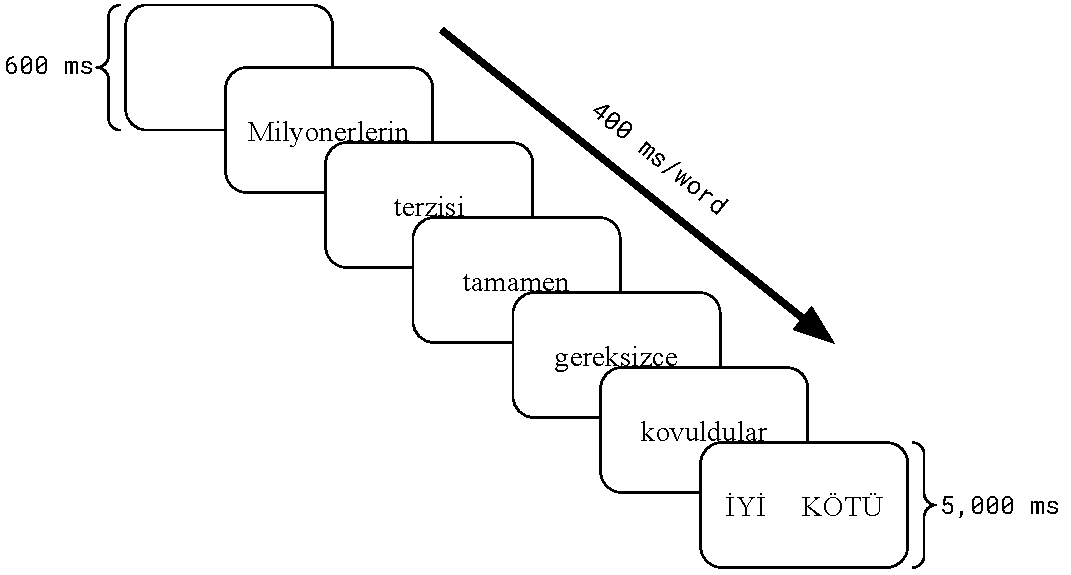
\includegraphics[width=\textwidth]{figure/trial_infographic.pdf}
    \caption{Simplified illustration of RSVP presentation utilized in the experiment}
    \label{fig:trial_infographic}
\end{figure}

\ea \label{ex:exp1_question}
Bu c\"umle kula\u{g}{\i}n{\i}za nas{\i}l geliyor? \\*
`How does this sentence sound to you?'
\z

The possible answers that participants could provide were either \emph{iyi} (good) or \emph{k\"ot\"u} (bad). Participants were asked to press the key P to indicate that a sentence is acceptable/good and Q to indicate that the sentence is unacceptable/bad. Within instructions before the experiments, they were told to provide judgments as soon as possible. If they did not respond within 5,000 ms during the experiment, the trial timed out, and participants were shown the message `\emph{Please respond faster!}' in red font.

Participants saw 40 experimental and 40 filler sentences. Experimental sentences were distributed among four different lists according to a Latin-square design. Every participant saw one version of the experiment with a specific list and one item per condition while seeing all filler items. All items were shuffled, and shuffling was done automatically by the Ibex Farm.

\subsection{Analysis}

Since our central question in this experiment was to test whether or not the existing agreement attraction finding was a product of the local ambiguity in \cites{LagoEtAl2019} experimental sentences due to morphological syncretism, we included \cites{LagoEtAl2019} data to our experimental data. We carried out the Bayesian analysis on our findings in Experiment 1 and on \cites{LagoEtAl2019} findings. As an additional categorical variable, we included the experiment (\citeand{LagoEtAl2019} / Our Experiment) in our Bayesian GLMs.

We excluded some participants using two criteria: (i) their performance in sentences with a singular attractor and (ii) their response time. For all participants, we found their mean percentage of \textit{yes} responses for singular attractor ungrammatical (\ref{ex:exp1-sgpl}) and singular attractor grammatical conditions (\ref{ex:exp1-sgsg}). If the difference between these mean values were below 0.25, that is, they failed to detect ungrammaticality even when there is no attractor to interfere, we excluded all data coming from that participant. In addition, we also excluded trials in which participants were not fast enough to respond ($RT > $ 4999 ms) or participants responded too quickly ($RT < $ 200 ms). After applying these criteria, 11.06\% of the trials from our experiment and 2.38\% of the \cites{LagoEtAl2019} trials. 

We analyzed yes responses with two Bayesian Generalized Linear Models (GLMs). We assumed that responses were distributed following a Bernoulli distribution with a probit link function. We used the R packages brms \citep{R-brms_a,R-brms_b} and rstan \citep{R-rstan} to fit Bayesian hierarchical models \citep[e.g.,][]{GelmanHill:2007, NicenboimVasishth:2016}. We analyzed only experimental sentences without including the missing data in the formula and used three categorical predictors and their interactions. Our predictors included: (i) sentence grammaticality ($c\_ung$), (ii) attractor number ($c\_att$), and (iii) presence of local ambiguity (i.e., experiment) ($c\_cons$). We used by-participant and by-item intercepts and slopes for all predictors and their interactions. We also included the log transformed trial number in our models ($l\_trial$). 

All factors were sum-coded. We used 0.5 for the following levels: the presence of local ambiguity, ungrammaticality, attractor plurality. As discussed in Chapter \ref{ch:intro}, we used semi-informative priors following. Our priors for our first model can be found in Table \ref{tab:exp1M1_priors}.

\begin{table}[hbt!]
    \caption{Priors for Our First Model in Experiment 1}
    \vspace{10pt}
    \begin{tabular}{ll}
      \hline
        Prior         & Parameter                \\\hline
        \emph{Normal}(-4,1)  & c\_ung                   \\
        \emph{Normal}(1,0.5) & c\_ung:c\_att            \\
        \emph{Normal}(0,1)   & Rest of the coefficients \\
        \emph{Normal}(0,1)  & Intercept\\
        \emph{LKJ}(2)        & All correlations         \\
        \emph{Cauchy}\textsuperscript{\it +}(0,1)   & All standard deviations \\ \hline
    \end{tabular}
  
    \label{tab:exp1M1_priors}
\end{table}

Since the effect we are looking for can either be formulated as the interaction between ungrammaticality and the plural attractor and the main effect of a plural attractor in ungrammatical sentences, we fitted an additional maximal model to yes responses of only ungrammatical conditions using the categorical predictors the presence of a plural attractor and local ambiguity as well as their interactions. Our prior specifications can be found in Table \ref{tab:exp1M2_priors}.


\begin{table}[hbt!]
    \caption{Priors for Our Second Model in Experiment 1}
    \vspace{10pt}
    \begin{tabular}{ll}
      \hline
        Prior         & Parameter                \\\hline
        \emph{Normal}(0,1)   & All coefficients \\
        \emph{Normal}(0,1)  & Intercept\\
        \emph{LKJ}(2)        & All correlations         \\
        \emph{Cauchy}\textsuperscript{\it +}(0,1)   & All standard deviations \\ \hline
    \end{tabular}
  
    \label{tab:exp1M2_priors}
\end{table}


\subsection{Results}

In this section, we provide summaries of the coefficient posterior distributions. We ran 4 chains with 1000 warm-up iterations and 4000 sampling iterations for our models. Our results report the posterior probability of the effect of coefficient $\beta$ being outside of the ROPE region, either smaller than $-0.1$ (\emph{P}($\beta < -0.1$)) or bigger than $0.1$ (\emph{P}($\beta > 0.1$)). If a distribution is completely outside of this area, we can say that we have definitive evidence for an effect. If it covers the practical equivalence area, we can say that according to our data, there seems to be no evidence for an effect. On occasions in which only a part of the distribution resides in the area, we explicitly quantify our degree of belief towards an effect. 

Accuracy of our grammatical filler items were exceptionally low (M = 0.35, SE = 0.01). On the other hand, the accuracy was quite high in ungrammatical fillers (M = 0.92, SE = 0.01). We checked whether or not a group of participants were responsible for this low accuracy in grammatical fillers. If that was the case, we could exclude those participants. However, Figure \ref{fig:exp1gFillHistogram} shows that the problem was not related to our participant group instead related to our items. Most of the participants were below 0.5, as clearly shown in the histogram.

\begin{knitrout}
\definecolor{shadecolor}{rgb}{0.969, 0.969, 0.969}\color{fgcolor}\begin{figure}[hbt!]

{\centering 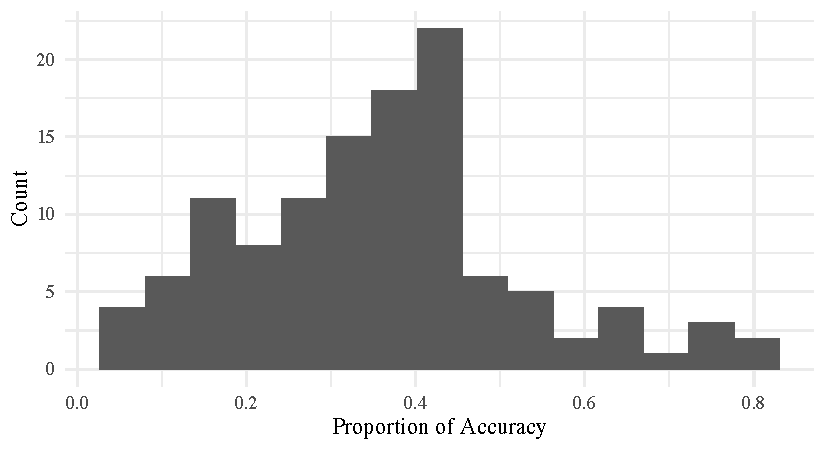
\includegraphics[width=\linewidth]{figure/exp1gFillHistogram-1} 

}

\caption[The accuracy histogram of grammatical fillers in Experiment 1]{The accuracy histogram of grammatical fillers in Experiment 1}\label{fig:exp1gFillHistogram}
\end{figure}

\end{knitrout}

Figure \ref{fig:exp1AvgResponse} shows the average proportions of acceptable responses as a function of sentence grammaticality, attractor number, and experiment. Since we were specifically interested in whether or not there would be a difference in acceptability due to a local ambiguity, we grouped the averages into two facets according to the grammaticality of the sentence. By doing so, we have the categorical experiment (presence of local ambiguity) in the x-axis, making comparison easier. Additionally, the line type shows the attractor number.  

\begin{knitrout}
\definecolor{shadecolor}{rgb}{0.969, 0.969, 0.969}\color{fgcolor}\begin{figure}[hbt!]

{\centering 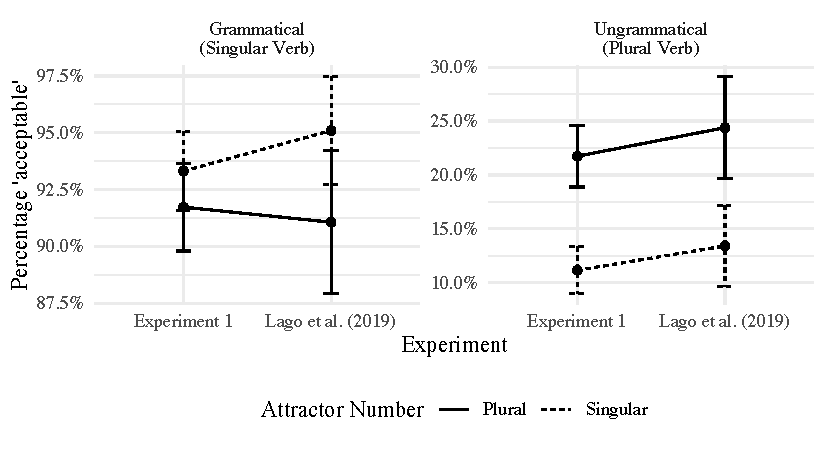
\includegraphics[width=\linewidth]{figure/exp1AvgResponse-1} 

}

\caption[The average percentage of acceptable responses according to the experimental conditions in our Experiment 1 and Lago et al.'s (2019) study]{The average percentage of acceptable responses according to the experimental conditions in our Experiment 1 and Lago et al.'s (2019) study}\label{fig:exp1AvgResponse}
\end{figure}

\end{knitrout}

With grammatical verbs, participants in both our experiment and \cites{LagoEtAl2019} study showed similar patterns. Accuracy rates were nearly equal (M = 0.92 and 0.93, SE = 0.01 and 0.01, for singular and plural attractors respectively) both in our experiment and in \cites{LagoEtAl2019} study (M = 0.91 and 0.95, SE = 0.02 and 0.01, for singular and plural attractors, respectively).

When we focus on our experimental results, we see that participants gave more acceptable responses in ungrammatical sentences with plural attractors (M = 0.22, SE = 0.01) compared to ungrammatical sentences with singular attractors (M = 0.11, SE = 0.01). The magnitude of the effect of plural attractor on ungrammatical sentences (0.11) were comparable to the \cites{LagoEtAl2019} results (0.11).

Figure \ref{fig:exp1RT} shows the average response times for correct responses as a function of sentence grammaticality, attractor number, and experiment. We have used the same layout as the one we used in \ref{fig:exp1AvgResponse}.

% \begin{knitrout}
% \definecolor{shadecolor}{rgb}{0.969, 0.969, 0.969}\color{fgcolor}\begin{figure}[hbt!]
% {\centering 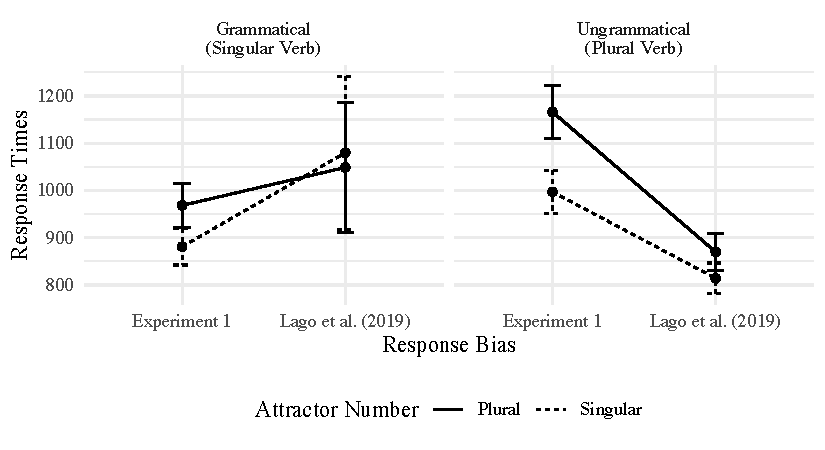
\includegraphics[width=\linewidth]{figure/exp1RT-1} 

% }

% \caption{The average response times according to the experimental conditions in our Experiment 1 and Lago et al.'s (2019) study}\label{fig:exp1RT}
% \end{figure}

% \end{knitrout}

\begin{figure}[hbt!]
{\centering 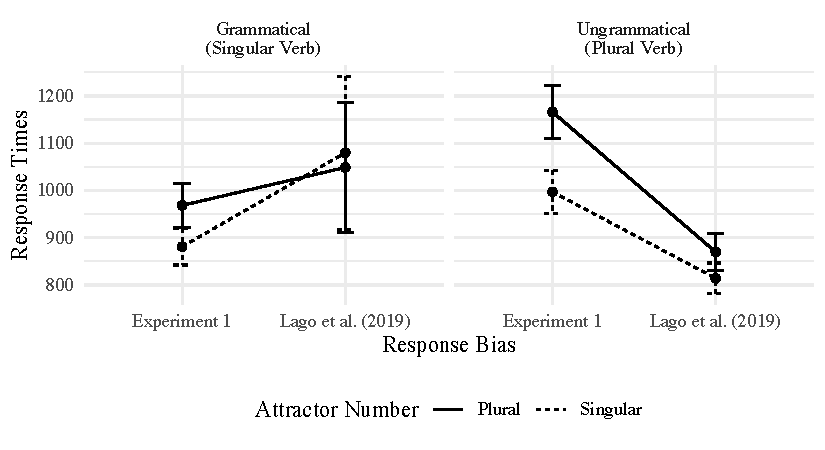
\includegraphics[width=\linewidth]{figure/exp1RT-1} 
}

\caption{The average response times according to the experimental conditions in our Experiment 1 and Lago et al.'s (2019) study}\label{fig:exp1RT}
\end{figure}


Our results suggest an overall slowdown in plural attractor conditions. This slowdown is evident in ungrammatical sentences. Participants gave faster responses when sentences include a singular attractor (M = 997.02, SE = 23.11) compared to a plural attractor (M = 1165.92, SE = 28.97). 


In Figure \ref{fig:exp1BayesPool}, we see the posterior probabilities for our Bayesian GLM model with a probit link, as well as ROPE borders and the probability of coefficients being smaller than $-0.1$. We used sentences from both our experiment and \cites{LagoEtAl2019} experiment. The negative main effect of ungrammaticality ($\hat{\beta}=-3.10;$ $CI=[-3.37; -2.86];$ $P(\beta>0.1)< .001$) indicated that participants were able to detect ungrammaticality both in our and \cites{LagoEtAl2019} experiment. Additionally, the positive interaction between the ungrammaticality and the plural attractor ($\hat{\beta}=0.76;$ $CI=[0.46; 1.04];$ $P(\beta>0.1)> .999$) meant that participants, on average, gave more \textit{yes} responses in ungrammatical sentences when there is a plural attractor. According to the posterior distribution of the coefficient trial no ($\hat{\beta}=0.03;$ $CI=[-0.05; 0.11];$ $P(\beta>0.1)   .04$), we infer that the order participants saw the experimental data did not affect the number of yes responses. Most importantly, a lack of evidence for the three-way interaction between the ambiguity, ungrammaticality, and the plural attractor ($\hat{\beta}=0.26;$ $CI=[-0.25; 0.76];$ $P(\beta>0.1)   .74$) suggested that the local ambiguity did not affect the grammaticality illusion. In other words, the magnitude of a plural attractor's effect in ungrammatical sentences was not contingent on the local ambiguity.

% \begin{knitrout}
% \definecolor{shadecolor}{rgb}{0.969, 0.969, 0.969}\color{fgcolor}\begin{figure}[hbt!]
% {\centering 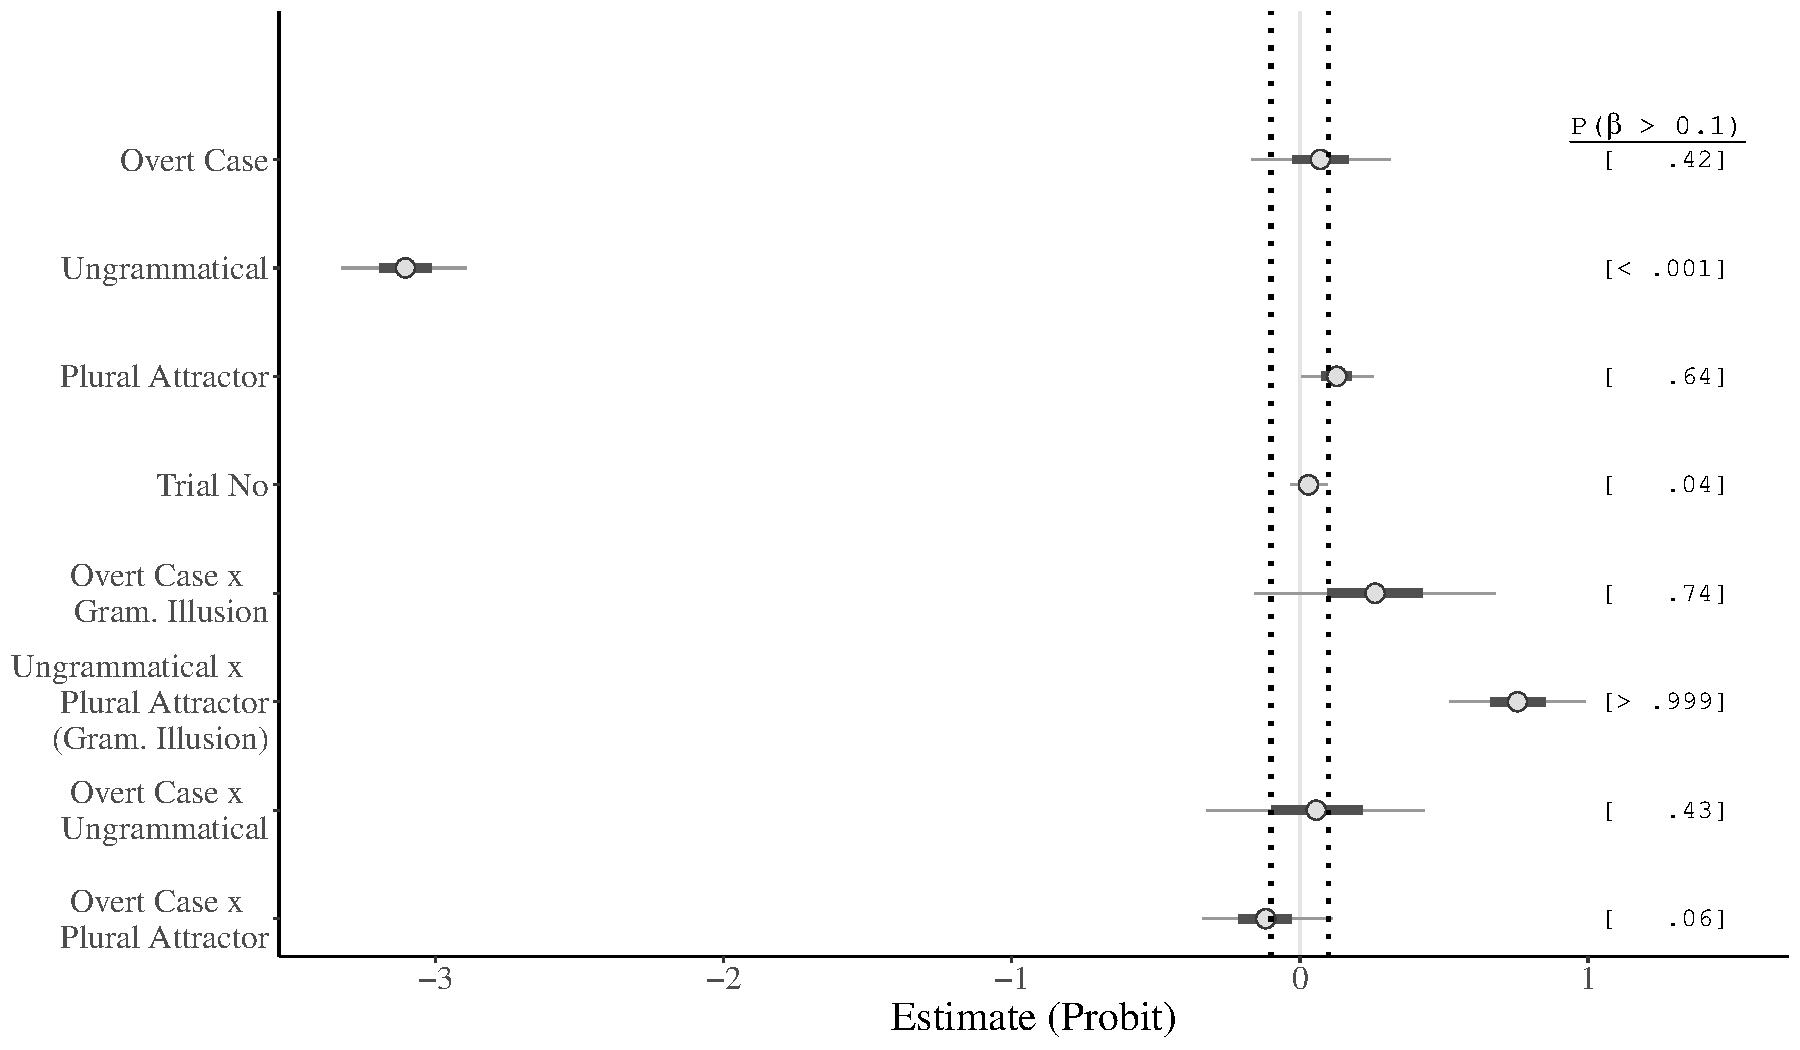
\includegraphics[width=\linewidth]{figure/exp1BayesPool-1} 
% }
% \caption{Estimates and 95\% credible intervals for the probit regression coefficients for the model of responses in our experiment and \citet{LagoEtAl2019}}\label{fig:exp1BayesPool}
% \end{figure}
% \end{knitrout}

\begin{figure}[hbt!]
{\centering 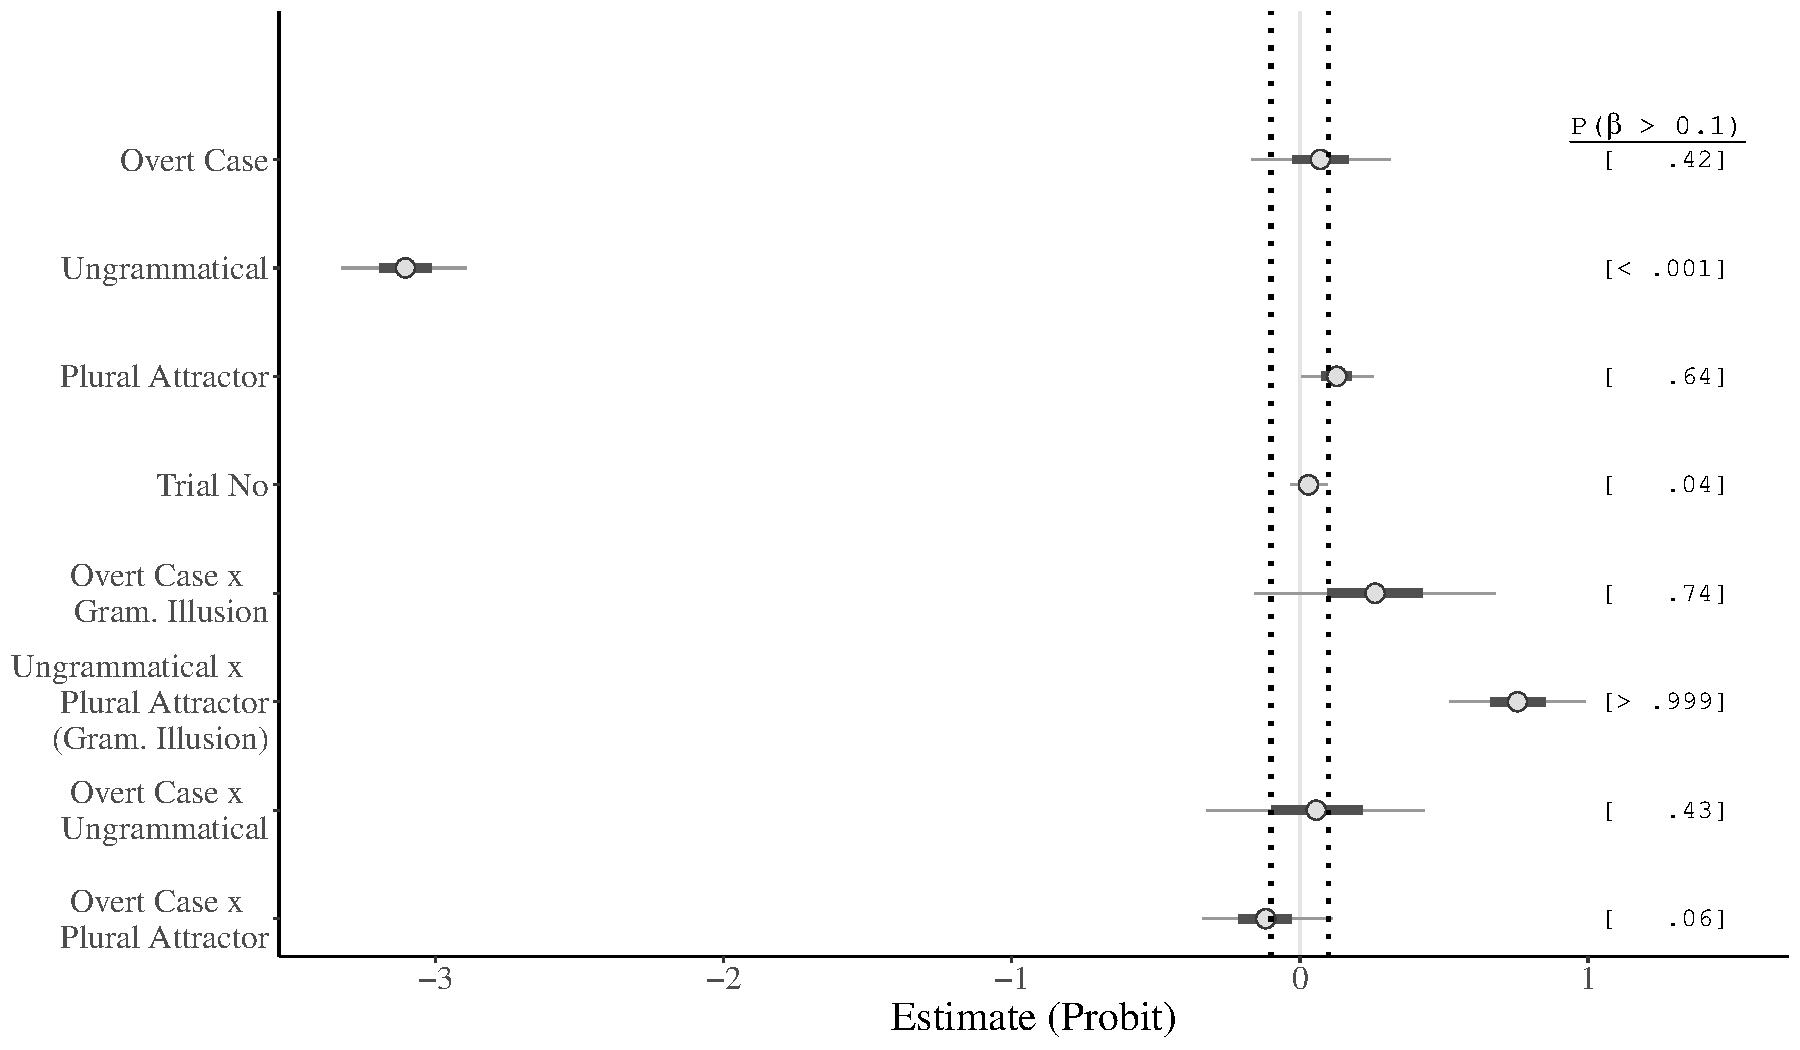
\includegraphics[width=\linewidth]{figure/exp1BayesPool-1} 
}
\caption[Estimates and 95\% credible intervals for the probit regression coefficients for the model of responses in our experiment and Lago et al. (2019)]{Estimates and 95\% credible intervals for the probit regression coefficients for the model of responses in our experiment and \citet{LagoEtAl2019}}\label{fig:exp1BayesPool}

\end{figure}

Figure \ref{fig:exp1BayesUngram} shows the estimates of a model based on only the ungrammatical sentences from both studies. The lack of evidence presented in \ref{fig:exp1BayesPool} is also supported in this model. Our second model showed no evidence for an interaction between the local ambiguity and the presence of a plural attractor ($\hat{\beta}=0.02;$ $CI=[-0.30; 0.34];$ $P(\beta>0.1)   .32$). Our second model also showed no main effect for the order of trials presented ($\hat{\beta}=-0.04;$ $CI=[-0.14; 0.07];$ $P(\beta>0.1)  .006$) and for the ambiguity ($\hat{\beta}=0.03;$ $CI=[-0.32; 0.38];$ $P(\beta>0.1)   .35$), meaning that independent of the presence of plural attractor local ambiguity did not affected the percentage of yes responses. Lastly, a more evidence for the plural attractor ($\hat{\beta}=0.48;$ $CI=[0.30; 0.67];$ $P(\beta>0.1)> .999$) were present in our second model compared to the first model. We infer from this difference that the ungrammatical sentences mainly drove the main effect of the plural attractor in the first model.


\begin{knitrout}
\definecolor{shadecolor}{rgb}{0.969, 0.969, 0.969}\color{fgcolor}\begin{figure}[hbt!]

{\centering 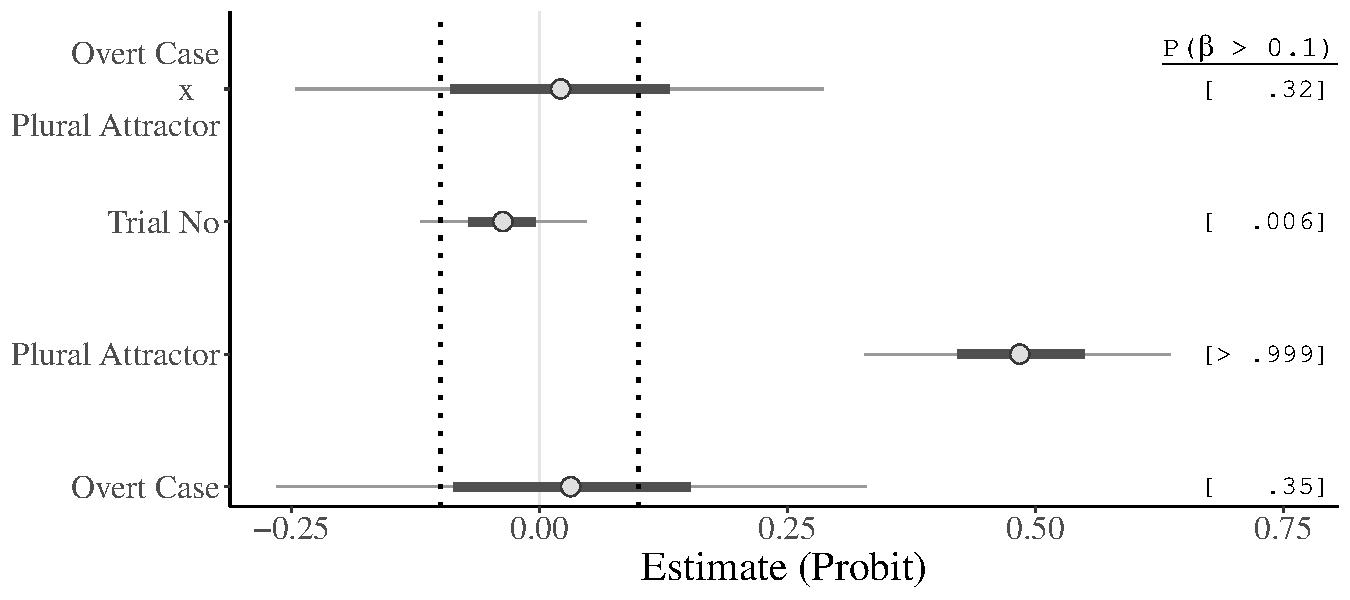
\includegraphics[width=\linewidth]{figure/exp1BayesUngram-1} 

}

\caption[Estimates and 95\% credible intervals for the probit regression coefficients for the model of responses to ungrammatical sentences in our experiment and Lago et al. (2019)]{Estimates and 95\% credible intervals for the probit regression coefficients for the model of responses to ungrammatical sentences in our experiment and \citet{LagoEtAl2019}}\label{fig:exp1BayesUngram}
\end{figure}
\end{knitrout}

\section{Discussion}

This chapter examined the alternative hypothesis that might explain the Turkish agreement attraction findings with genitive-possessive constructions. We hypothesized that the local ambiguity due to the syncretism between the possessive and the accusative case in \cites{LagoEtAl2019} items might be the main factor in their findings. We argued that participants might posit two different parses when they encounter \emph{NP-\Gen{} NP-i} strings. They would associate the head \emph{NP-i} with a non-subject case in one possible parse. This, in turn, reduces the association between the head \emph{NP-i} and the subjecthood. If that was the case and the previous findings were due to the lingering association between the noun \emph{NP-i} and the objecthood, then we expected not to find an agreement attraction effects in sentences where the case on the head \emph{NP-i} is unambiguous.

Our results suggested that participants accepted ungrammatical sentences with plural attractors more often than ungrammatical sentences with singular attractors even when the subject head is disambiguated. This finding is comparable to mainstream agreement attraction and \cites{LagoEtAl2019} findings. 

Additionally, our initial Bayesian model showed no interaction between the grammaticality illusion (the agreement attraction) and the local ambiguity. That is, manipulating the presence of the local ambiguity did not change the acceptability difference between the plural attractor-ungrammatical and the singular-attractor ungrammatical conditions. Our second model, which only included ungrammatical sentences, verified these findings: there was no interaction between the local ambiguity and the attractor number. Our model results suggested that the agreement attraction was not contingent on the local ambiguity and the head NP's reduced association with the subjecthood due to lingering effects of alternative parses. 

In light of our findings and \cites{LagoEtAl2019} findings, existing agreement attraction findings cannot be explained via our hypothesis based on the inhibitory effects of a possible parse where a subject head is parsed as a direct object. Additionally, we can say that local ambiguities stemming from the marking on the head noun do not give rise to additional grammaticality illusions. Unlike previous findings on the role of case syncretism in agreement attraction \citep{Slioussar2018}, our results suggested that participants did not utilize cues based on the form. This difference was because the syncretism in \citeand{Slioussar2018} was introduced in the attractor, whereas the syncretism in our study was related to the marking on the subject head. It seemed that when the manipulation done on the syntactically more prevalent elements, participants did utilize abstract linguistic cues. Thus, our results point towards an attraction account where the syntactic difference between the head and the attractor plays a significant role.

\chapter{EXPERIMENT 2: AN INVESTIGATION OF SHALLOW PROCESSING} \label{ch:exp2}

The previous chapter focused on the role of local ambiguity in agreement attraction and investigated an alternative explanation for existing Turkish agreement attraction effects: reduced subjecthood association. Our results showed that the local ambiguity on the head noun does not seem to affect either the presence or the magnitude of the grammaticality illusion.

This chapter aims to investigate yet another explanation for existing Turkish agreement attraction effects: form-driven processing strategy. In the light of recent findings in psychology and psycholinguistics, one can stipulate that participants do not comprehend all details of lexical, semantic, or discourse-related information \citep{ChristiansonEtAl2001}. Instead, they may have a rough understanding of the sentence or use specific strategies to answer questions while having a limited understanding of the sentence. This chapter investigate whether participants both in our experiment and \cites{LagoEtAl2015} experiment were using additional strategies that relies on the phonological form. We present two experiments in which we abuse the homophony between the nominal and the verbal plural marking in Turkish. 

\section{Shallow processing in agreement attraction}

Having discussed an alternative hypothesis based on local ambiguity and reduced subjecthood association, we focus on another alternative theory that stems from Turkish' unique feature. Unlike other languages that exhibited agreement attraction effects, the Turkish verbal agreement marker and nominal plural marker share the same form: \emph{-lAr}. Consider the example in (\ref{ex:LARTease}) where both the attractor and the matrix verb is plural. 

\ea[*]{\label{ex:LARTease}
    \gll Milyoner-{ler}-in terzi-si tamamen gereksizce kov-ul-du-{lar}.\\
    millionaire-\Pl-\Gen{} tailor-\Poss{} completely without\_reason fire-\Pass-\Pst-\Tpl{}\\
    \glt `The millionaires' tailor were fired for no reason at all.'}
\z

If we assume that participants thoroughly analyze and understand the sentence, both \emph{-lAr} markings will be evaluated, and the features will be utilized to process the sentence. We expect (\ref{ex:LARTease}) to be detected as an unacceptable sentence when this thorough analysis is done. However, this is not the case, and all accounts explaining agreement attraction effects resort to erroneous analyses of the sentence to some degree. Thus, a general question like `\emph{Do participants always parse the sentence to its full extent?}' may arise, especially when the topic is speeded acceptability judgment tasks where most of the sentences follow a template and are very similar to each other. On some occasions, it is possible that participants may not have sufficient information to fully parse the sentence due to the reasons like environmental noise or experimental factors. Thus, another question, `\emph{How will they answer grammaticality judgment questions when they do not have sufficient information?}' arises. One possible answer to this question is guessing. If they guess the acceptability of a sentence with insufficient information, is this guessing always an uninformed guess, or can there be degrees of guessing? 

We argue that remembering the details of the noun that \emph{-lAr} is concatenated, only remembering that there was a suffix \emph{-lar} but not remembering its host, and not remembering two initial DPs at all would create different types of guessing procedures. While their guess would be completely uninformed if they do not remember two initial DPs, they may have more nuanced guessing if they remember the suffix \emph{-lAr} but do not remember its exact host. One way to represent these differences is by giving yes and no guesses different probabilities. Giving them both a 50\% probability to happen would mean that both of them are equally possible. On the other hand, we believe that the yes guess probability would increase if the participants remembered a suffix \emph{-lAr} instead of not remembering any detail corcerning initial DPs. 

On some other occasions, it is possible that participants do not check the whole sentence for judgment but instead check specific positions or specific dependencies only. They may not thoroughly analyze the entire sentence, and oversee irrelevant (concerning the given sentence) elements, such as adjuncts. Participants may create a strategy to answer the judgment questions as quickly and accurately as possible on those occasions. For example, suppose a speeded acceptability judgment experiment only has acceptable sentences with inanimate subjects. In that case, one can posit that participants will not process the whole sentence after a certain point; and when they see an inanimate subject and they will deem the sentences grammatical immediately. 

The homophony we introduced in (\ref{ex:LARTease}) creates a unique opportunity to test the possibility of these aforementioned processes in agreement attraction: guessing via shallow processing and task-related strategies, i.e., form-driven processing strategy. We hypothesized that readers might engage in an shallow process in a similar fashion described above. According to our hypothesis, readers have insufficient information to judge the sentence reliably on some occasions. When such situation arises, readers try to guess the acceptability of the sentence since they are in a forced choice experiment. We argue that this guessing process has an underlying mechanism as specified in Figure \ref{fig:mptModel}.
\begin{figure}[hbt!]
    \centering
    \noindent
    \begin{forest}
    mpt, EL
    [,coordinate
        [target\\ item,no edge
            [recollection\\ certainity, EL=r
                [no]
            ]
            [recollection\\ uncertainty, EL=1-r,
                [guess yes, tier=L1, EL=g,
                    [yes]
                ]
                [guess no, tier=L1, EL=1-g
                    [no]
                ]
            ]
        ]
        [,coordinate, no edge]
        [target\\ item, no edge
            [guess yes, tier=L1, EL=g,
                    [yes]
            ]
            [guess no, tier=L1, EL=1-g
                [no]
            ]
        ]
    ]
    \end{forest} 
    \caption{Proposed multinomial processing tree of sentence processing}\label{fig:mptModel}
\end{figure}

Sometimes, they will not have any information concerning the sentence due to an attentional lapse. On those occasions, they will simply select randomly either yes or no answers. In Figure \ref{fig:mptModel}, we specify giviny yes responses in such states with $g$ possibility and no with $1-g$ possibility, given that $1<g<0$. 

On other occasions, in which the participants have some information concerning the sentence, we argue that their answer will depend on whether or not they remember the exact host of the nominal suffix \emph{-lAr}. We specify that with $r$ possibility they will remember the exact host of the suffix, given that $1<r<0$. When they remember the exact host, they will successfully parse the sentence and give the correct answer no. 

However, when they do not relocate the host of the suffix with $1-r$ possibility, they will rely on the guessing the answer to the grammaticality judgment question. For simplicity reasons, we assume the same guessing parameter $g$. Even though, we assume the same parameter, this guessing will be more informed. The probability of giviny yes responses in such cases is not simply $g$, but $(1-r){\ }\times{\ }g$. 

Via using a multinomial processing tree as in Figure \ref{fig:mptModel}, we explicitly state that agreement attraction effects, in other words giving yes responses to ungrammatical target items with plural attractors, results from a shallow processing with form-driven guessing elements.

\section{Experiment 2A}

Experiment 2A aims to control for form-driven processing strategies that the participants may employ in the processing of Turkish number agreement. A processing mechanism driven by the form itself, rather than the embedded linguistic features, would predict the comparable agreement attraction effects even when the attractor does not contain a possible nominal plural feature to create interference but contains a form-identical morpheme. To this end, we utilized homophony between nominal and verbal plural marking in Turkish. Instead of genitive marked nouns as we did in Experiment 1, we used the verb of an object relative clause as an attractor (\ref{ex:exp2Tease}). We expect that under some conditions in which participants do not have sufficient information to rate sentences (un)acceptable, they will decide on the grammaticality of the sentence based on their memory of plural morpheme string, regardless of the feature itself. 

\ea \label{ex:exp2Tease}
    \gll {Tut-tuk-\O/lar-(n){\i}} {a\c{s}\c{c}{\i}} mutfak-ta s{\"u}rekli z{\i}pla-d{\i}-\O/lar.\\
    hire-\Nmlz{}-\Sg{}/\Pl{}-\Poss{} cook kitchen-\Loc{} non-stop jump-\Pst{}-\Sg{}/\Pl{}\\
    \glt `The cook that they hired\textsubscript{SG/PL} jumped\textsubscript{SG/PL} in the kitchen non-stop.'
\z


\subsection{Participants}

Our participants (N = 80) were native Turkish speakers and Bo\u{g}azi\c{c}i University undergraduate students. In exchange for attending the experiment, they were given extra credit in one of the pre-determined Linguistics courses. The average age of participants was 21, ranging from 18 to 31. The principles of the Declaration of Helsinki and the regulations concerning research ethics at Bo\u{g}azi\c{c}i University were followed without any exception. Before the experiment, all participants were asked to provide informed consent. During the experiment, any information regarding their identities was not collected. 


\subsection{Materials}

We have formed 40 sets of items. The grammaticality of the sentences (\textit{grammatical} x \textit{ungrammatical}) and the number marking of the attractor (\textit{singular} x \textit{plural}) was manipulated. Unlike Experiment 1, we used nominalized relative clause attractors instead of nouns. We took advantage of homophony between Turkish nominal and verbal plural markers. Both morphemes spell out as \textit{-lAr}, enabling us to check whether an extremely shallow dependency parsing based on the forms of morphemes rather than abstract features can explain agreement attraction in Turkish.

All experimental sentences followed the same template as the experiment one except for the nature of the attractor: $RC(-PL){\ }{\ }DP[NOM]{\ }{\ }Adjunct{\ }{\ }VP(-PL)$. All sentences started with a complex subject DP like `\textit{the cook that they hired \ldots{}}' (\textit{tuttuklar{\i} a\c{s}\c{c}{\i}}), in which the verb of the relative clause functioned as the attractor. Because the head noun was singular in all conditions, sentences with plural verb agreement were ungrammatical. We have used the same verbs as Experiment 1 and have not changed the verb types' distribution. We also utilized the same or extremely similar adverbials in length. We did not manipulate the number of the head noun and manipulated the number marking on the attractor. The relative clauses we used in this experiment are all object relative clauses, and they are all marked with canonical \textit{-dIK} nominalizer. Since Turkish is a pro-drop language, we also dropped the subject within the embedded clause, thus ending up with a one-word object relative clause whose head is also the controller of the number agreement on the matrix verb. One example set of experimental items can be seen in \ref{ex:exp2items}.

\ea \label{ex:exp2items}
    \ea[*]{{Plural Attractor, Ungrammatical (Plural Verb)} \label{ex:exp2-plpl}\\*
    \gll [{Tut-tuk-lar-{\i}} {a\c{s}\c{c}{\i}}] mutfak-ta sürekli z{\i}pla-d{\i}-lar.\\
    hire-\Nmlz{}-\Pl{}-\Poss{} cook kitchen-\Loc{} non-stop  jump-\Pst{}-\Pl{}\\
    \glt `The cook that they hired\textsubscript{\Pl{}} jumped\textsubscript{\Pl{}} in the kitchen non-stop.'}
    \ex[]{{Plural Attractor, Grammatical (Singular Verb)} \label{ex:exp2-plsg} \\*
    \gll [{Tut-tuk-lar-{\i}} {a\c{s}\c{c}{\i}}] mutfak-ta sürekli z{\i}pla-d{\i}.\\
    hire-\Nmlz{}-\Pl{}-\Poss{} cook kitchen-\Loc{} non-stop  jump-\Pst{}\\
    \glt `The cook that they hired\textsubscript{\Pl{}} jumped\textsubscript{\Sg{}} in the kitchen non-stop.'}
    \ex[*]{{Singular Attractor, Ungrammatical (Plural Verb)} \label{ex:exp2-sgpl}\\*
    \gll [{Tut-tu\u{g}-u} {a\c{s}\c{c}{\i}}] mutfak-ta sürekli z{\i}pla-d{\i}-lar.\\
    hire-\Nmlz{}-\Poss{} cook kitchen-\Loc{} non-stop  jump-\Pst{}-\Pl{}\\
    \glt `The cook that they hired\textsubscript{\Sg{}} jumped\textsubscript{\Pl{}} in the kitchen non-stop.'}
    \ex[]{{Singular Attractor Grammatical (Singular Verb)} \label{ex:exp2-sgsg}\\*
    \gll [{Tut-tu\u{g}-u} {a\c{s}\c{c}{\i}}] mutfak-ta sürekli z{\i}pla-d{\i}.\\
    hire-\Nmlz{}-\Poss{} cook kitchen-\Loc{} non-stop  jump-\Pst{}\\
    \glt `The cook that they hired\textsubscript{\Sg{}} jumped\textsubscript{\Sg{}} in the kitchen non-stop.'}
    \z
\z

We have modified our filler sentences. In our filler items for Experiment 2, we ensured that every sentence starts with an object relative clause. We used plural-marked RCs with grammatical verbs and singular RCs with ungrammatical verbs. In all of our filler sentences, the dependency between the first DP subject and its verb is resolved in an embedded sentence which fuctions as an adverbial. Grammatical filler items in Experiment 2 all had a template of $RC-(PL){\ }{\ }DP[NOM]{\ }{\ }Adverb{\ }{\ }Converb{\ }{\ }Noun{\ }{\ }Adverb{\ }{\ }Verb-(PL)$, whereas ungrammatical filler items used a template of $RC-(SG){\ }{\ }DP[NOM]{\ }{\ }Adverb{\ }{\ }Converb{\ }{\ }Noun{\ }{\ }Adverb{\ }{\ }Verb-(SG)$

Similar to Experiment 1, half of our fillers were with an overt plural marking on a grammatical verb while the other half were without an overt plural marking on an ungrammatical verb. We wanted to avoid a possible strategy where participants use plural ending as a direct indication of ungrammaticality. We used Turkish pro-drop characteristics, which enable participants to form a dependency between the matrix verb and the null subject. Example filler sentences can be seen in \ref{ex:exp2fillers}. All of our experimental and filler items can be found in Appendix \ref{ap:exp2aitems}. 

\ea \label{ex:exp2fillers}
    \ea[]{\label{ex:exp2fillers-g} {Grammatical Filler (Plural Verb)}\\* 
        \gll Oku-t-tuk-lar-{\i} {\"o}\u{g}renci ba\c{s}ar{\i}l{\i} ol-unca mutlu ol-du-lar.\\ 
        read-\Caus{}-\Nmlz{}-\Pl{}-\Poss{}  student successful be-\Nmlz{} happy be-\Pst{}-\Pl{}\\
        \glt `When the student they sponsored become successful, they became happy.'}
    \ex[*]{\label{ex:exp2fillers-ung} {Ungrammatical Filler (Singular Verb)}\\* 
        \gll Kand{\i}r-d{\i}\u{g}-{\i} adam {\"o}de-me-yince bula\c{s}{\i}k saatlerce y{\i}ka-d{\i}.\\ 
        trick-\Nmlz{}-\Poss{}  man pay-\Neg{}-\Nmlz{} dish for.hours clean-\Pst{}\\
        \glt Intended:`When the man he tricked did not pay, he cleaned dishes for hours.'}
    \z
\z



\subsection{Procedure}

Experiment 2A was carried out in the same manner as Experiment 1. 

\subsection{Analysis}

In our analysis, we used the items from Experiment 1 and Experiment 2. This decision was made to answer our hypothesis about whether participants use the form of the plural suffix rather than the linguistic features. A presence of interaction between the attractor type (\textit{nominal} vs. \textit{verbal}) and the agreement attraction effect would indicate that people use the linguistic features rather than the form of the plural suffix. We also fitted an additional model where we only used Experiment 2 data to check the interaction between the presence of a plural RC attractor and the grammaticality. 

Similar to Experiment 1, we removed the data for all participants who did not exceed the threshold of 0.25 percentage points in `yes' responses between the grammatical condition and the ungrammatical condition with singular attractors. We also excluded data based on participants' response times in the same manner as Experiment 1. As a result, we excluded 5.39\% of trials from the Experiment 2A, and 11.06\% of trials from Experiment 1.

We analyzed yes responses with two Bayesian Generalized Linear Models (GLMs). We assumed that responses were distributed following a Bernoulli distribution with a probit link function. We used the R packages brms \citep{R-brms_a,R-brms_b} and rstan \citep{R-rstan} to fit Bayesian hierarchical models \citep[e.g.,][]{GelmanHill:2007, NicenboimVasishth:2016}. 

In our first model, we included experimental items from our first experimentt as well. We analyzed only experimental sentences without including the missing data in the formula and used three categorical predictors and their interactions. We used (i) grammaticality of the sentence, (ii) attractor number, and (iii) category of the attractor (i.e. the experiment), as well as their interactions as predictors. We also included the log transformed trial number in our models. Moreover, we used by-participant and by-item intercepts and slopes for all predictors. All factors were sum-coded. We used 0.5 for the following levels: (i) ungrammaticality, (ii) plural attractor, and (iii) genitive-marked nominal modifier. 

We have used the same priors that were specified in the analysis of Experiment 1. We also fit an additional model to see the effect of verbal attractors in Turkish agreement attraction. In our second model we only used experimental conditions from our second experiment. 


\subsection{Results}

In this section, we provide summaries of the coefficient posterior distributions. We ran 4 chains with 1000 warm-up iterations and 4000 sampling iterations for our models. Our results report the posterior probability of the effect of coefficient $\beta$ being outside of the ROPE region, either smaller than $-0.1$ (\emph{P}($\beta < -0.1$)) or bigger than $0.1$ (\emph{P}($\beta > 0.1$)). If a distribution is completely outside of this area, we can say that we have definitive evidence for an effect. If it covers the practical equivalence area, we can say that according to our data, there seems to be no evidence for an effect. On occasions in which only a part of the distribution resides in the area, we explicitly quantify our degree of belief towards an effect. 

Both grammatical and ungrammatical fillers' accuracy were fairly high (M = 0.94 and 0.92, SE = 0.01 and 0.01 for grammatical and ungrammatical fillers). It suggests that participants could differentiate grammatical and ungrammatical sentences from each other.

Figure \ref{fig:exp2AvgResponse} shows the average proportions of acceptable responses by experimental conditions for Experiment 2A, Experiment 1, and \cites{LagoEtAl2019} study. We divided the results into two facets: grammatical and ungrammatical sentences. We have the attractor type (i.e., experiments) on the x-axis. Finally, the attractor number is represented with the line type. 

\begin{knitrout}
\definecolor{shadecolor}{rgb}{0.969, 0.969, 0.969}\color{fgcolor}\begin{figure}[hbt!]

{\centering 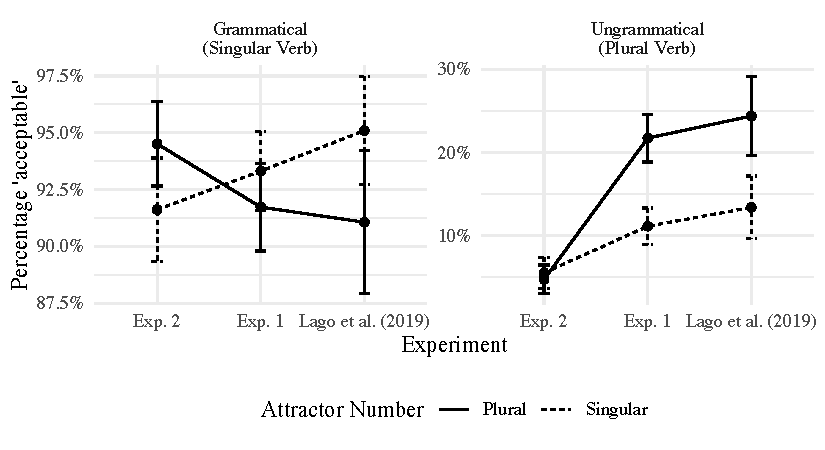
\includegraphics[width=\linewidth]{figure/exp2AvgResponse-1} 

}

\caption[The average percentage of acceptable responses according to the experimental conditions in Experiment 1, Experiment 2A, and Lago et al.'s (2019) study]{The average percentage of acceptable responses according to the experimental conditions in Experiment 1, Experiment 2A, and Lago et al.'s (2019) study}\label{fig:exp2AvgResponse}
\end{figure}

\end{knitrout}

We see that our results were comparable with previous findings of Turkish agreement attractions. Even though it is unusual that grammatical sentences with singular attractors (M = 0.92, SE = 0.01) compared to grammatical sentences with plural attractors (M = 0.95, SE = 0.01), given the standard errors, the difference between these two conditions do not seem to be significant. 

As for ungrammatical sentences, the mainstream agreement attraction effect, i.e., the effect of plural attractor on the acceptability of ungrammatical sentences was not present in Experiment 2. In Experiment 2, the ungrammatical sentences with plural attractors are rated as acceptable (M = 0.05, SE = 0.01) as their counterparts with singular attractors (M = 0.06, SE = 0.01). The lack of effect (0.01\%) compared to the magnitude of the effect in Experiment 1 (0.11\%) and \cites{LagoEtAl2019} study (0.11\%) indicates that the verbal plural morpheme does not trigger an illusionary agreement.

Figure \ref{fig:exp2RT} shows the average response times for correct responses by experimental conditions for our Experiment 2, Experiment 1, and \cites{LagoEtAl2019} study. We have used the same layout as the one we used in Figure \ref{fig:exp2AvgResponse}. However, this time we located Experiment 2 in the middle so that its relation to both our Experiment 1 and \cites{LagoEtAl2019} study can be observed easily.

\begin{knitrout}
\definecolor{shadecolor}{rgb}{0.969, 0.969, 0.969}\color{fgcolor}\begin{figure}[hbt!]

{\centering 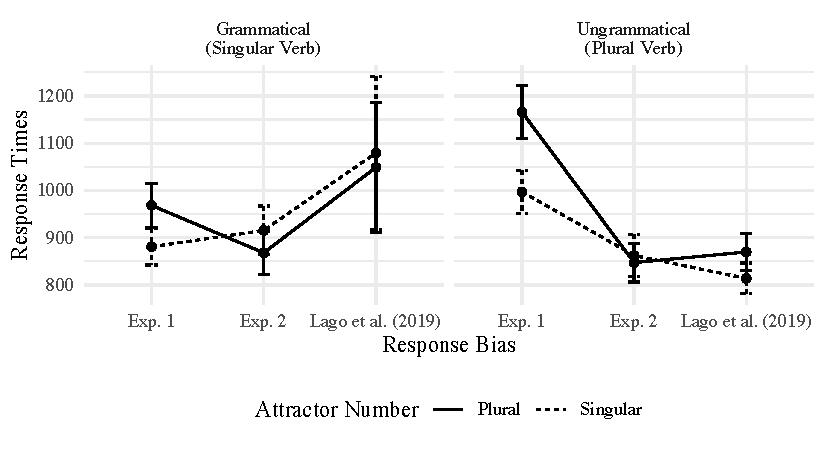
\includegraphics[width=\linewidth]{figure/exp2RT-1} 

}

\caption[The average response times according to the experimental conditions in Experiment 1, Experiment 2A, and Lago et al.'s (2019) study]{The average response times according to the experimental conditions in Experiment 1, Experiment 2A, and Lago et al.'s (2019) study}\label{fig:exp2RT}
\end{figure}

\end{knitrout}

Response Times in our Experiment 2 do neither align with our Experiment 1 nor with \cites{LagoEtAl2019} study fully. In the grammatical sentence, response times are comparable to our Experiment 1; however, the relation between the singular and plural attractor conditions is again reversed. Overall, participants took more time answering acceptability judgment questions to grammatical sentences with singular attractor (M = 915.28, SE = 26.32) compared to their plural attractor counterpart (M = 867.91, SE = 23.43). This difference does not seem to be substantial.

Within ungrammatical conditions, the picture is distinctively different from our findings in Experiment 1. There is no slowdown due to the presence of a plural attractor. Grammaticality judgment questions in both singular and plural attractor conditions were answered in a similar time (M = 862.31 and 847.23, SE = 22.82 and 20.87 for singular and plural attractor conditions, respectively). 

In Figure \ref{fig:exp2BayesPool}, we present the coefficient posterior summaries extracted from our Bayesian GLM fitted to the data from Experiment 1 and Experiment 2A. 


\begin{knitrout}
\definecolor{shadecolor}{rgb}{0.969, 0.969, 0.969}\color{fgcolor}\begin{figure}[hbt!]

{\centering 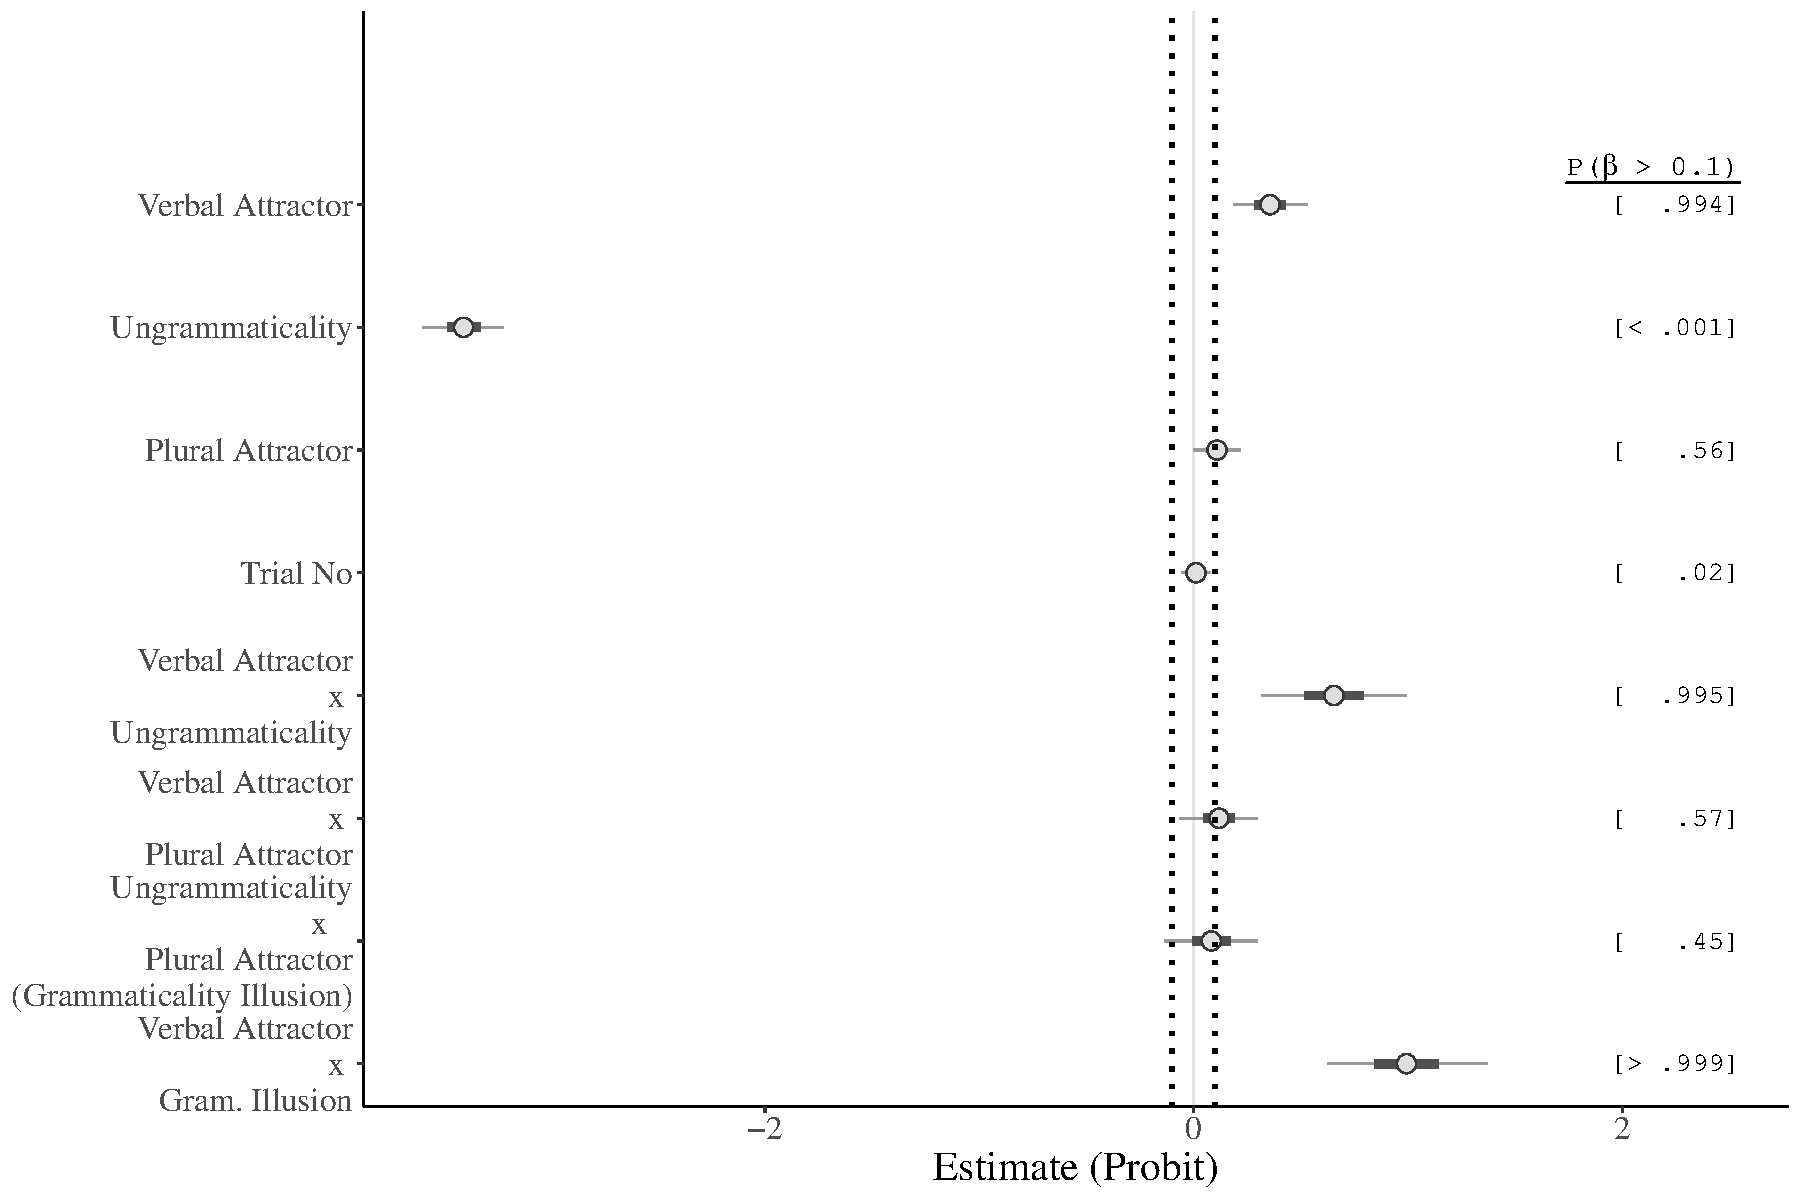
\includegraphics[width=\linewidth]{figure/exp2BayesPool-1} 

}

\caption[Estimates and 95\% credible intervals for the probit regression coefficients for the model of responses in Experiment 1 and Experiment 2A]{Estimates and 95\% credible intervals for the probit regression coefficients for the model of responses in Experiment 1 and Experiment 2A}\label{fig:exp2BayesPool}
\end{figure}

\end{knitrout}
The negative main effect of ungrammaticality ($\hat{\beta}=-3.41;$ $CI=[-3.64; -3.19];$ $P(\beta>0.1)< .001$) suggests that participants gave detected the ungrammaticality easily. The positive main effect of the genitive-marked nominal modifier ($\hat{\beta}=0.36;$ $CI=[0.15; 0.56];$ $P(\beta>0.1)  .994$) suggest that participants overall have more difficulty in correctly judging ungrammatical sentences in the presence of a nominal attractor compared to a verbal one. The positive interaction between the genitive-marked nominal attractor and the ungrammaticality ($\hat{\beta}=0.65;$ $CI=[0.25; 1.06];$ $P(\beta>0.1)  .995$) showed that participants made more errors in ungrammatical sentences when the nominal attractor is present instead of a verbal attractor independent of the presence of a plural attractor. More importantly, the positive three-way interaction ($\hat{\beta}=0.99;$ $CI=[0.55; 1.45];$ $P(\beta>0.1)> .999$) implies that the effect of nominal modifiers was even more amplified when they judge ungrammatical sentences with plural attractors compared to their counterparts with singular attractors. 

% font and resizing. May 1 11:51



Figure \ref{fig:exp2Bayesonly2} shows the estimates of our model fitted only to the data from Experiment 2. While Figure \ref{fig:exp2BayesPool} indicates the greater magnitude of agreement attraction effects with genitive attractors, it does not clearly show whether or not there exists a grammaticality illusion with verbal attractors. The negative interaction between grammaticality and plural attractor ($\hat{\beta}=-0.25;$ $CI=[-0.65; 0.17];$ $P(\beta>0.1)   .05$) shows that the presence of a plural marked verbal element in the vicinity of the head noun made participants give yes responses less often as opposed to having a singular marked verbal element. This interaction can also be interpreted as an amplified number of yes responses in grammatical sentences with plural attractors. 


\begin{knitrout}
\definecolor{shadecolor}{rgb}{0.969, 0.969, 0.969}\color{fgcolor}\begin{figure}[hbt!]

{\centering 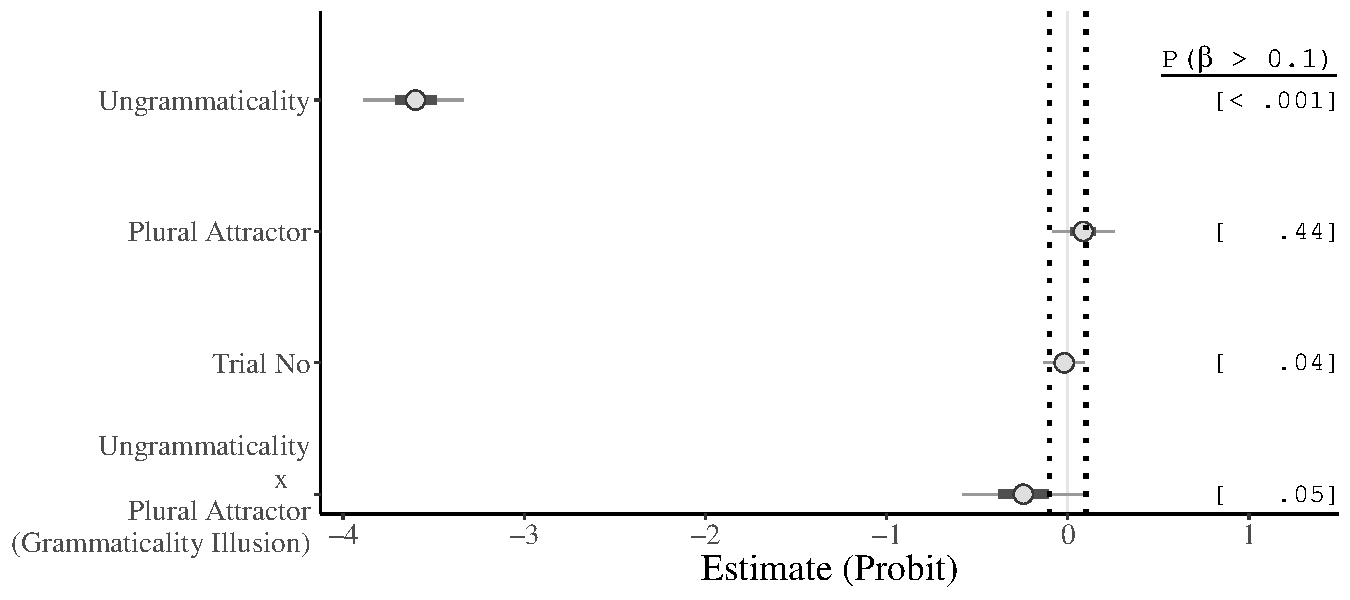
\includegraphics[width=\linewidth]{figure/exp2Bayesonly2-1} 

}

\caption[Estimates and 95\% credible intervals for the probit regression coefficients for the model of responses in Experiment 2 only]{Estimates and 95\% credible intervals for the probit regression coefficients for the model of responses in Experiment 2 only}\label{fig:exp2Bayesonly2}
\end{figure}

\end{knitrout}

\subsection{Discussion}


Experiment 2A examined an alternative hypothesis for Turkish agreement attraction facts. We hypothesized that participants might have formed a form-driven processing strategy and employed a shallow processing in the previous experiments. Assuming that most of the yes responses in ungrammatical conditions come from guesses, either completely random guesses or slightly informed ones, we argued that participants might solely rely on the foggy memory of a plural-marking in the sentence. On some occasions, where they misremembered the host of the plural-marking, they might erroneously judge sentences grammatical even though the head was singular. 

Results of our speeded acceptability judgment experiment showed that verbs of reduced object relative clauses were not appropriate attractors and there was no attraction effects with verbal attractors. However, number agreement attractions were observed in our previous experiment when the attractors were nominal. Even though the surface morphological form was identical for both verbal and nominal plural morphemes, the contributions of these two \emph{-lAr} morphemes to attraction effects differed. This finding contradicted our hypothesized form-driven processing strategy and supported an account of agreement attraction based on abstract linguistic features, rather than mere forms.

However, one possible explanation for Experiment 2 results is that participants never considered \emph{-lAr} morpheme to be hosted by a controller. They neither had any item that contained a plural head noun nor any experimental condition which would induce an erroneous agreement. Given that nominal attractors embedded more deeply in relative clauses than prepositional phrases cause less agreement attraction effects, a visible effect of an embedded verbal attractor in our experiment would be highly improbable. We believe that a limited number of grammatical filler items where the initial RC was marked with a plural agreement was not enough to lead participants to correlate the suffix \emph{-lAr} and the grammaticality potentially. 

Given these reasons, we pooled experimental conditions from Experiment 1 and 2A and conducted another study with eight conditions (Grammaticality x Attractor Number x Attractor Type). We already observed that in two different populations (\citeand{LagoEtAl2019} and Experiment 1), genitive-marked attractors cause agreement attraction and erroneous subject-verb agreement. In the light of previous findings that suggest participants misinterpret the sentence and compute the attractors as the head noun \citep{PatsonHusband2016}, we hypothesized that participants would misinterpret some of the ungrammatical sentences with genitive-marked attractors, and thus create form-based strategies more easily after seeing a certain number of ungrammatical conditions with plural-marked genitive modifiers. 

\section{Experiment 2B}

The aim of Experiment 2B is to again check for form-driven processing strategies but in a possibly more enabling experimental context. We believe that the presence of experimental conditions that possibly provide the necessary grammaticality illusion for participants to form a response strategy would give rise to mainstream attraction effects in relevant conditions with the embedded verbal attractor. Experiment 2B also provided a direct comparison in a single population between the nominal and embedded verbal attractor, which was also lacking in Experiment 2A.

\subsection{Participants}

Our participants (N = 95) were native Turkish speakers and Bo\u{g}azi\c{c}i University undergraduate students. In exchange for attending the experiment, they were given extra credit in one of the pre-determined Linguistics courses. The average age of participants was 21, ranging from 18 to 30. The principles of the Declaration of Helsinki and the regulations concerning research ethics at Bo\u{g}azi\c{c}i University were followed without any exception. Before the experiment, all participants were asked to provide informed consent. During the experiment, any information regarding their identities was not collected. 

\subsection{Materials}

In Experiment 2B, we have used 40 sets of experimental sentences where we manipulated the number of the attractor, the number agreement of the main verb, and the type of the attractor. We combined experimental items from Experiment 1 and 2A. We made sure that all eight conditions were minimally different. However, some of the items from Experiment 1 did not have the same head noun-matrix verb pair with those from Experiment 2A. For this reason, we modified some of the Experiment 1 sentences minimally. One item set is given below in (\ref{ex:exp2bitems}), where the subject phrase is marked with square brackets, and the dependency between the subject head and the matrix verb is signaled using bold-face.

\ea \label{ex:exp2bitems}
    \ea[*]{{Plural Verbal Attractor, Ungrammatical (Plural Verb)} \label{ex:exp2b-rcplpl}\\*
        \gll [{Tut-tuk-lar-{\i}} {a\c{s}\c{c}{\i}}] mutfak-ta sürekli z{\i}pla-d{\i}-lar.\\
        hire-\Nmlz{}-\Pl{}-\Poss{} cook kitchen-\Loc{} non-stop  jump-\Pst{}-\Pl{}\\
        \glt `The cook that they hired\textsubscript{\Pl{}} jumped\textsubscript{\Pl{}} in the kitchen non-stop.'}
    \ex[]{{Plural Verbal Attractor, Grammatical (Singular Verb)} \label{ex:exp2b-rcplsg} \\*
        \gll [{Tut-tuk-lar-{\i}} {a\c{s}\c{c}{\i}}] mutfak-ta sürekli z{\i}pla-d{\i}.\\
        hire-\Nmlz{}-\Pl{}-\Poss{} cook kitchen-\Loc{} non-stop  jump-\Pst{}\\
        \glt `The cook that they hired\textsubscript{\Pl{}} jumped\textsubscript{\Sg{}} in the kitchen non-stop.'}
    \ex[*]{{Singular Verbal Attractor, Ungrammatical (Plural Verb)} \label{ex:exp2b-rcsgpl}\\*
        \gll [{Tut-tu\u{g}-u} {a\c{s}\c{c}{\i}}] mutfak-ta sürekli z{\i}pla-d{\i}-lar.\\
        hire-\Nmlz{}-\Poss{} cook kitchen-\Loc{} non-stop  jump-\Pst{}-\Pl{}\\
        \glt `The cook that they hired\textsubscript{\Sg{}} jumped\textsubscript{\Pl{}} in the kitchen non-stop.'}
    \ex[]{{Singular Verbal Attractor Grammatical (Singular Verb)} \label{ex:exp2b-rcsgsg}\\*
        \gll [{Tut-tu\u{g}-u} {a\c{s}\c{c}{\i}}] mutfak-ta sürekli z{\i}pla-d{\i}.\\
        hire-\Nmlz{}-\Poss{} cook kitchen-\Loc{} non-stop  jump-\Pst{}\\
        \glt `The cook that they hired\textsubscript{\Sg{}} jumped\textsubscript{\Sg{}} in the kitchen non-stop.'}
    \ex[*]{{Plural Nominal Attractor, Ungrammatical (Plural Verb)} \label{ex:exp2b-genplpl}\\*
        \gll [{Y{\"o}netici-ler-in} {a\c{s}\c{c}{\i}-s{\i}}] mutfak-ta sürekli z{\i}pl-d{\i}-lar.\\
        manager-\Pl{}-\Gen{} cook-\Poss{} kitchen-\Loc{} non-stop  jump-\Pst{}-\Pl{}\\
        \glt `The millionaries' cook jumped\textsubscript{\Pl{}} in the kitchen non-stop.'}
    \ex[]{{Plural Nominal Attractor, Grammatical (Singular Verb)} \label{ex:exp2b-genplsg} \\*
        \gll [{Y{\"o}netici-ler-in} {a\c{s}\c{c}{\i}-s{\i}}] mutfak-ta sürekli z{\i}pl-d{\i}.\\
        manager-\Pl{}-\Gen{} cook-\Poss{} kitchen-\Loc{} non-stop  jump-\Pst{}\\
        \glt `The millionaries' cook jumped\textsubscript{\Sg{}} in the kitchen non-stop.'}
    \ex[*]{{Singular Nominal Attractor, Ungrammatical (Plural Verb)} \label{ex:exp2b-gensgpl}\\*
        \gll [{Y{\"o}netici-nin} {a\c{s}\c{c}{\i}-s{\i}}] mutfak-ta sürekli z{\i}pl-d{\i}-lar.\\
        manager-\Gen{} cook-\Poss{} kitchen-\Loc{} non-stop  jump-\Pst{}-\Pl{}\\
        \glt `The millionarie's cook jumped\textsubscript{\Pl{}} in the kitchen non-stop.'}
    \ex[]{{Singular Nominal Attractor, Grammatical (Singular Verb)} \label{ex:exp2b-gensgsg}\\*
        \gll [{Y{\"o}netici-nin} {a\c{s}\c{c}{\i}-s{\i}}] mutfak-ta sürekli z{\i}pl-d{\i}.\\
        manager-\Gen{} cook-\Poss{} kitchen-\Loc{} non-stop  jump-\Pst{}\\
        \glt `The millionarie's cook jumped\textsubscript{\Sg{}} in the kitchen non-stop.'}
    \z
\z

In addition to 40 experimental items, we also included 40 filler items, half of which are ungrammatical. We used the same filler items from Experiment 2A and did not modify any part of the fillers. All of our experimental and filler items can be found in Appendix \ref{ap:exp2bitems}.

\subsection{Procedure}

Experiment 2B was carried out in the same manner as Experiment 1 and 2A. 

\subsection{Analysis}

Since our main question was that participants used a response strategy based on form-matching and our Experiment 2B included both verbal and nominal attractors, we used only the experimental items from Experiment 2B. 

Similar to Experiment 1 and 2B, we removed all participants who did not exceed the threshold of 0.25 percentage points in yes responses between the grammatical condition and the ungrammatical condition with singular attractors. We also excluded trials where participants either gave too fast ($RT < $ 200 ms) or too slow ($RT > $ 4999 ms) responses. As a result, we excluded 2.34\% of trials from Experiment 2B.

We fitted two Bayesian GLMs to the yes responses from our Experiment 2B. While our first model included all experimental conditions, the second one only had verbal attractor conditions. We assumed that responses were distributed following a Bernoulli distribution with a probit link function. We used the R packages brms \citep{R-brms_a,R-brms_b} and rstan \citep{R-rstan} to fit Bayesian hierarchical models \citep[e.g.,][]{GelmanHill:2007, NicenboimVasishth:2016}. We analyzed only experimental sentences without including the missing data in the formula and used three categorical predictors and their interactions. We used (i) grammaticality of the sentence, (ii) attractor number, and (iii) the attractor type, as well as their interactions as predictors. We also included the log transformed trial number in our models ($l\_trial$). Moreover, we used by-participant and by-item intercepts and slopes for all predictors. All factors were sum-coded. We used 0.5 for the following levels: (i) ungrammaticality, (ii) plural attractor, and (iii) genitive-marked nominal modifier. We used the same priors as we used in previous Bayesian GLMs.

\subsection{Results}

In this section, we provide summaries of the coefficient posterior distributions. We ran 4 chains with 1000 warm-up iterations and 4000 sampling iterations for our models. Our results report the posterior probability of the effect of coefficient $\beta$ being outside of the ROPE region, either smaller than $-0.1$ (\emph{P}($\beta < -0.1$)) or bigger than $0.1$ (\emph{P}($\beta > 0.1$)). If a distribution is completely outside of this area, we can say that we have definitive evidence for an effect. If it covers the practical equivalence area, we can say that according to our data, there seems to be no evidence for an effect. On occasions in which only a part of the distribution resides in the area, we explicitly quantify our degree of belief towards an effect.

Both grammatical and ungrammatical fillers' accuracy were high (M = 0.95 and 0.94, SE = 0.01 and 0.01 for grammatical and ungrammatical fillers). We believe that our filler items served their purpose, and participants paid attention to the experiment. 

Figure \ref{fig:exp2bAvgResponse} shows the average proportions of acceptable responses for each experimental condition in Experiment 2B. We divided the results into two facets: grammatical and ungrammatical sentences. We have the attractor type (Genitive modifiers vs. Relative Clause modifiers as attractors) on the x-axis. Finally, the attractor number is represented with the line type. 

\begin{knitrout}
\definecolor{shadecolor}{rgb}{0.969, 0.969, 0.969}\color{fgcolor}\begin{figure}[hbt!]

{\centering 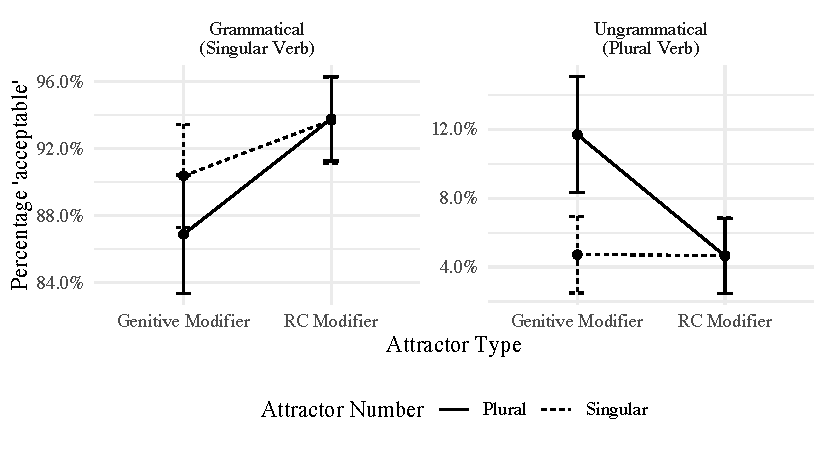
\includegraphics[width=\linewidth]{figure/exp2bAvgResponse-1} 

}

\caption[The average percentage of acceptable responses according to the experimental conditions in Experiment 2B]{The average percentage of acceptable responses according to the experimental conditions in Experiment 2B}\label{fig:exp2bAvgResponse}
\end{figure}

\end{knitrout}


In grammatical sentences, the overall acceptability was lower in genitive modifier conditions (ME = 0.87 and 0.9, SE = 0.02 and 0.02, for singular and plural attractors, respectively) compared to RC modifier conditions (ME = 0.94 and 0.94, SE = 0.01 and 0.01, for singular and plural attractors, respectively). 

In ungrammatical sentences, the plurality of the attractor did not change the overall attractor within RC modifier conditions (ME = 0.05 and 0.05, SE = 0.01 and 0.01, for singular and plural attractors, respectively). On the other hand, the attractor number mattered when the modifier was  a genitive-marked nominal. Participants accepted ungrammatical sentences with a plural genitive-marked nominal attractor (ME = 0.12, SE = 0.02) more often compared to the ones with a singular attractor (ME = 0.05, SE = 0.01). Even though this effect size (0.07) diminished compared to our previous agreement attraction findings (0.11), they were still comparable. This decrease in acceptability can be seen in Figure \ref{fig:exp2B1AvgResponse}. The layout in Figure \ref{fig:exp2B1AvgResponse} is the same as the previous figures. Differently from the rest, the x-axis represents the attractor type and the experiment.  

\begin{knitrout}
\definecolor{shadecolor}{rgb}{0.969, 0.969, 0.969}\color{fgcolor}\begin{figure}[hbt!]

{\centering 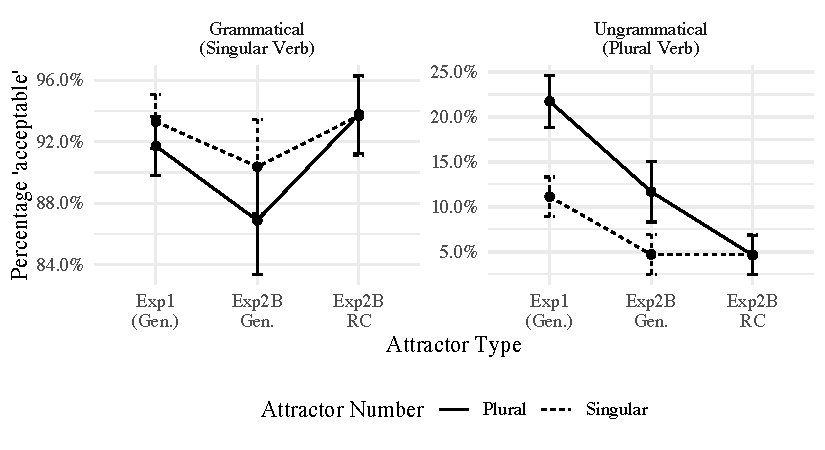
\includegraphics[width=\linewidth]{figure/exp2B1AvgResponse-1} 

}

\caption[The average percentage of acceptable responses according to the experimental conditions in Experiment 1 and Experiment 2B]{The average percentage of acceptable responses according to the experimental conditions in Experiment 1 and Experiment 2B}\label{fig:exp2B1AvgResponse}
\end{figure}

\end{knitrout}

Figure \ref{fig:exp2bRT} shows average response times for correct responses in Experiment 2B. We have used the same layout as in Figure \ref{fig:exp2bAvgResponse}.

\begin{knitrout}
\definecolor{shadecolor}{rgb}{0.969, 0.969, 0.969}\color{fgcolor}\begin{figure}[hbt!]

{\centering 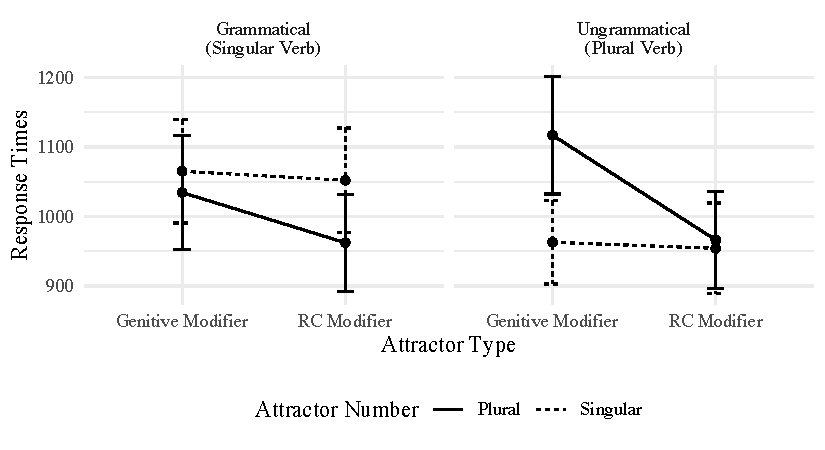
\includegraphics[width=\linewidth]{figure/exp2bRT-1} 

}

\caption[The average response times according to the experimental conditions in Experiment 2B]{The average response times according to the experimental conditions in Experiment 2B}\label{fig:exp2bRT}
\end{figure}

\end{knitrout}

Participants in our Experiment 2B responded faster to grammatical sentences with plural-marked attractors (M = 1034.45 and 962.22, SE = 41.88 and 35.55 for genitive and RC modifiers, respectively) compared to the ones with singular ones (M = 1065.04 and 1051.99, SE = 37.92 and 38.48 for genitive and RC modifiers, respectively). 

As for ungrammatical conditions, participants gave correct responses slower with plural genitive modifier (M = 1116.92, SE = 43.09) than the singular genitive modifier (M = 962.85, SE = 30.56). However, this difference in RT was not present in RC modifier conditions (M = 954.04 and 966.21, SE = 33.28 and 35.69 for singular and plural RCs, respectively). 


In Figure \ref{fig:exp2bBayes}, we present the coefficient posterior summaries from our Bayesian GLM fitted to experimental sentences from Experiment 2B. 


\begin{figure}[hbt!]

{\centering 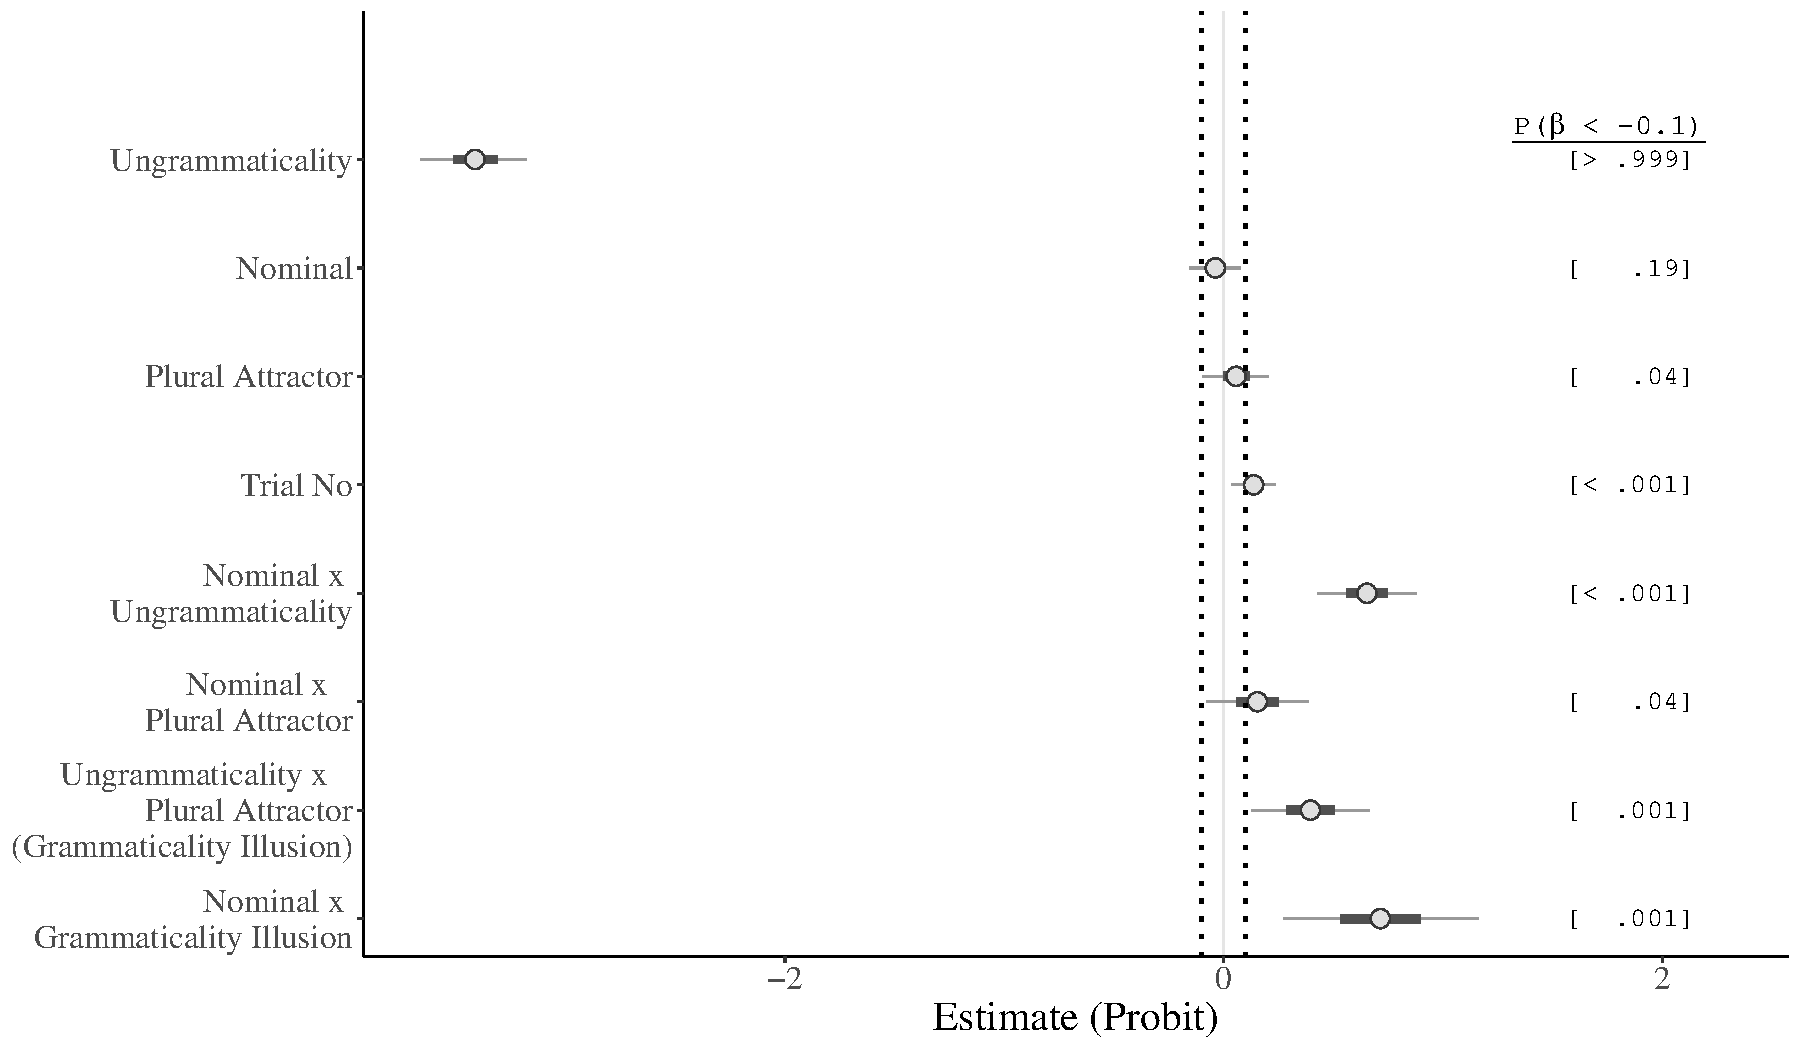
\includegraphics[width=\linewidth]{figure/exp2bBayes-1} 

}

\caption[Estimates and 95\% credible intervals for the probit regression coefficients for the model of responses in Experiment 2B]{Estimates and 95\% credible intervals for the probit regression coefficients for the model of responses in Experiment 2B}\label{fig:exp2bBayes}
\end{figure}

The negative main effect of ungrammaticality ($\hat{\beta}=-3.41;$ $CI=[-3.72; -3.14];$ $P(\beta< -0.1)> .999$) was also present in this Bayesian GLM as well. Participants were able to differentiate between the grammatical and ungrammatical items within experimental items. Our posterior summaries showed a positive effect of the trial number ($\hat{\beta}=0.14;$ $CI=[0.02; 0.26];$ $P(\beta< -0.1)< .001$), meaning that as participants see more experimental items, they gave more yes responses, on average. This effect suggested that participants might change how they answered questions as they proceeded in the experiment. The positive three-way interaction between the type of the attractor, ungrammaticality, and the plurality of the attractor ($\hat{\beta}=0.71;$ $CI=[0.18; 1.26];$ $P(\beta< -0.1)=   .001$) implied that the mainstream attraction effect (Ungrammaticality * Plural Attractor interaction) was amplified when the attractor is a genitive-marked nominal modifier.


However, this three-way interaction did not prove that people exhibited agreement attraction effects with verbal modifiers. Figure \ref{fig:exp2bRCBayes} shows coefficient posteriors for our second Bayesian GLM, fitted only the experimental items with verbal modifiers. We see that there was an evidence for neither an effect of plural attractor ($\hat{\beta}=-0.07;$ $CI=[-0.41; 0.25];$ $P(\beta< -0.1)=    .42$) nor an interaction between the ungrammaticality and the plural attractor ($\hat{\beta}=0.25;$ $CI=[-0.29; 0.82];$ $P(\beta< -0.1)=    .10$). 

\begin{knitrout}
\definecolor{shadecolor}{rgb}{0.969, 0.969, 0.969}\color{fgcolor}\begin{figure}[hbt!]

{\centering 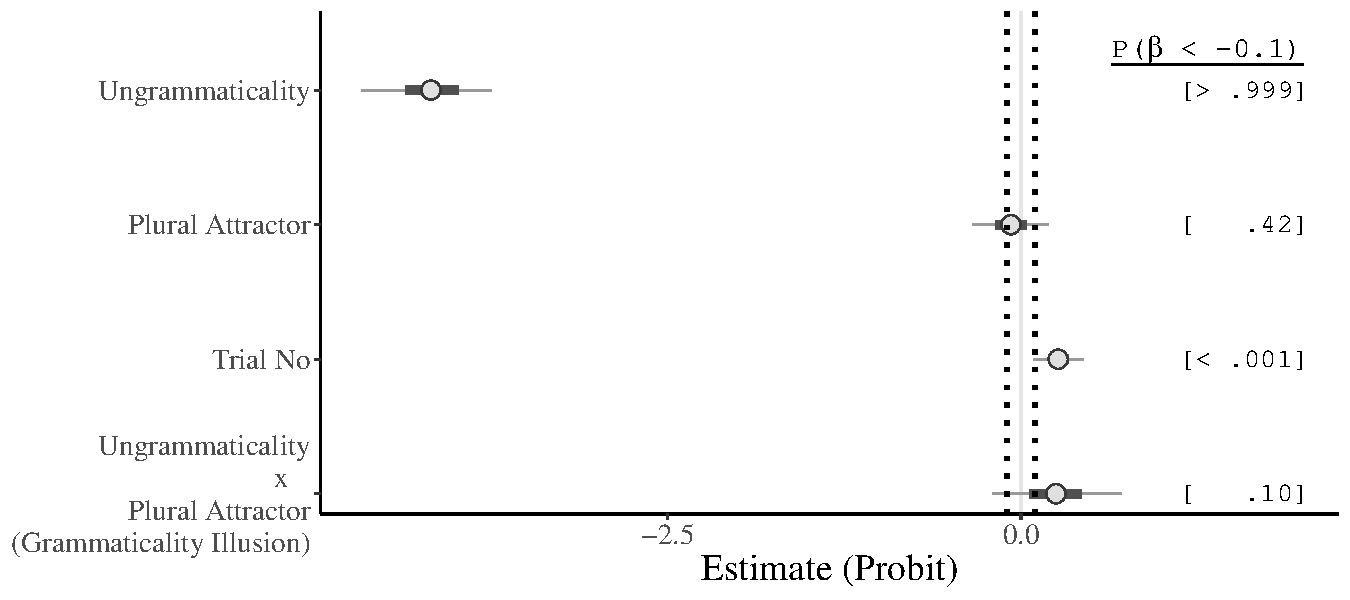
\includegraphics[width=\linewidth]{figure/exp2bRCBayes-1} 

}

\caption[Estimates and 95\% credible intervals for the probit regression coefficients for the model of responses to RC conditions in Experiment 2B]{Estimates and 95\% credible intervals for the probit regression coefficients for the model of responses to RC conditions in Experiment 2B}\label{fig:exp2bRCBayes}
\end{figure}

\end{knitrout}

\subsection{Discussion}

In Experiment 2B, we re-examined our hypothesis, according to which participants may form a response strategy using a form-matching mechanism. Even though our previous study, Experiment 2A, showed no evidence for such a strategy, we wanted to verify these findings with a new experiment. One possibility is that since there was no agreement controller with plural marking in Experiment 2A, participants might have never considered the form-matching response strategy. We included additional conditions, with genitive-marked modifiers which might lead participants to erroneously deem plural attractor DPs as agreement controllers and consider that the suffix \emph{-lAr} can be hosted by the head noun as well.

Our results showed that participants made significantly fewer errors in ungrammatical sentences when the attractor was verbal compared to nominal attractors. We successfully replicated our findings in Experiment 2A. Even though we included new genitive-modifier conditions to trigger agreement attraction effects in verbal attractors, it did not affect our participants. Together with Experiment 2A, Experiment 2B findings verified that our hypothesized decision-making process would not explain the patterns in Turkish agreement attraction effects.  

% The relationship with trial no and agreement attraction maybe?

\section{Discussion}

This chapter investigated another alternative hypothesis that might explain Turkish agreement attraction facts. We hypothesized that when participants did not have sufficient information to judge sentences' acceptability, they might use other heuristics such as form-matching strategies. Given that participants do not always process the sentences fully and utilize shallow processing methods, agreement attraction effects might be residual of a guessing mechanism. While some yes responses come from truly random guesses due to not having any memory regarding the subject-verb dependency, some yes responses come from educated guesses where participants have some sort of information that they can use. In our case, the additional information was the recollecting the presence of the plural suffix \emph{-lAr}. We argued that when people read sentences, sometimes they will remember and analyze the whole sentence. On the other hand, they will sometimes have a recollection uncertainty and misremember the host which the suffix \emph{-lAr} is concatenated. On those occasions, they will use a response strategy where they try to match two homophonous suffixes to answer grammaticality judgment questions.

Our MPT model differentiates these informed guesses from random guessing by either adjusting the relative probabilities of guessing yes ($g$) and no ($1-g$) or providing an additional probabilistic state before guessing. The product of this new state's probability and the standard guessing yes probability will be our way of formalizing the informed guesses ($(1-r){\ }\times{\ }g$). We conducted a speeded acceptability judgment experiment to test our hypothesis that participants with relocation uncertainty may utilize form-related response strategies. We investigated whether or not agreement-wise unrelated morphemes can trigger agreement attraction effects. We argued that if people utilize this form-driven processing strategy, they may give more yes responses even when there are verbal plural attractors in the vicinity compared to no plural attractor in the vicinity. We were able to test this hypothesis using Turkish since both verbal and nominal plurality is shown via the same morpheme: \emph{-lAr}.

Our results from two experiments, where we used verbs of a reduced object relative clauses as an attractor, showed that the usual effect of the plural attractor in ungrammatical sentences did not arise when the attractor is a verbal element. We expected that if participants were using our hypothesized response strategy, they would accept ungrammatical sentences with a plural attractor independent of the type of the attractor. However, this was not the case. Our findings contradicted our hypothesis and implied that participants used abstract linguistic features rather than form-related cues. Given our results, it was evident that the type of the attractor and the nature of the plural morpheme mattered in processing subject-verb dependencies. 

Moreover, our results from Experiment 2B showed a slight decrease in the overall percentage of yes responses in ungrammatical sentences with a nominal attractor. A possible explanation for this decrease might be the presence of verbal attractors. Their presence might have affected participants' sensitivity and made them more conservative in giving yes responses. The decrease in grammatical sentences supports this hypothesis. However, our experimental design and results are not equipped to answer this question. Thus, all we can say is that we have minimal evidence for such a speculation.

Lastly, we must note that our experiment designs were not without problems. Even though we compare the contributions of verbal and nominal attractors, they are not on par syntactically. We provide syntactic structures in (\ref{syntax:genposs}) and (\ref{syntax:orc}). To visualize syntactic differences between the structures, we mark the nodes between the root node and the node attractor is immediately dominated. The verbal attractor is embedded in a relative clause, consisting of DP, \emph{n}P, TP, \emph{v}P, and VP \citep{Aygen2002}. This relative clause is the modifier of the DP. On the other hand, the genitive-marked nominal modifier is the specifier of the determiner phrase, and it is immediately dominated by the root node \cite{OzturkTaylan2016}. It is clear that the syntactic distance between the root and the attractor nodes is more considerable with the verbal attractor.


\ea 
\ea \label{syntax:orc} {Object Relative Clause}\\*
\scalebox{1}{\begin{forest}
%fned
    [DP
        [DP
                [\emph{n}P
                    [TP
                        [DP\\\emph{pro}\textsubscript{j}]
                        [TP
                            [\emph{v}P
                                [DP\\\emph{t}\textsubscript{j}]
                                [\emph{v}P
                                    [VP
                                        [DP\\\emph{t}\textsubscript{i}]
                                    [V\\tuttuklar{\i}]
                                ]
                                [\emph{v}]
                            ]
                        ]
                        [T]
                    ]
                ]
                [\emph{n}]
            ]
            [D]
        ]
        [DP
            [NP [N\\a\c{s}\c{c}{\i}\textsubscript{i}] ]
            [D]
        ]
    ]
    \path[fill=black] (.parent anchor) circle[radius=2pt];
    \path[fill=black] (!1.child anchor) circle[radius=2pt];
    \path[fill=black] (!11.child anchor) circle[radius=2pt];
    \path[fill=black] (!111.child anchor) circle[radius=2pt];
    \path[fill=black] (!1112.child anchor) circle[radius=2pt];
    \path[fill=black] (!11121.child anchor) circle[radius=2pt];
    \path[fill=black] (!111212.child anchor) circle[radius=2pt];
    \path[fill=black] (!1112121.child anchor) circle[radius=2pt];
    \path[fill=black] (!11121212.child anchor) circle[radius=2pt];
\end{forest}}\vspace{2em}

\ex \label{syntax:genposs} {Genitive-Possessive DP}\\*
\scalebox{0.9}{\begin{forest}
    %fned
        [DP
            [DP\textsubscript{i}
                [PlP
                    [NP [NP\\Y\"onetici] ]
                    [Pl\\-ler]
                ]
                [D\\-in]
            ]
            [DP
                [\emph{n}P
                    [DP\\\emph{t}\textsubscript{i}]
                    [\emph{n}P
                        [NP [N\\a\c{s}\c{c}{\i}]]
                        [\emph{n}\\-s{\i}]
                    ]
                ]
                [D]
            ]
        ]
        \path[fill=black] (.parent anchor) circle[radius=2pt];
        \path[fill=black] (!1.child anchor) circle[radius=2pt];
        \path[fill=black] (!11.child anchor) circle[radius=2pt];
        \path[fill=black] (!112.child anchor) circle[radius=2pt];
    \end{forest}}
\z
\z


One reason for the failure of triggering grammaticality illusion in Experiment 2B might be the syntactic distance discrepancy between the conditions. Previous studies have shown that syntactic distance between the head and the modifier affects the magnitude of the attraction. The more embedded attractors resulted in smaller effects of plural attractors in ungrammatical sentences. A better experimental design for comparing between a nominal and a verbal attractor would include objects/subjects of an embedded RC instead of a genitive-marked nominal modifier that is not embedded under CP and TP. Even though there are multiple studies that shown clause-external attractors or attractors in embedded sentences induce agreement attraction, Turkish has not been tested yet.


\chapter{EXPERIMENT 3: AN INVESTIGATION OF RESPONSE BIAS}  \label{ch:exp3}

The previous chapters focused on the role of local ambiguity and response strategies and investigated possible explanations for existing Turkish agreement attraction effects. In those chapters, we have found that the effect of a plural attractor in ungrammatical sentences were not due to a local ambiguity stemming from a case syncretism or a possible form-matching response strategy. Even though both phenomenon have been important aspects of the psycholinguistics literature, it seems that they do not play a role in Turkish agreement attraction given our data and analysis.

Another influential topic in psycholinguistics is the response bias. This chapter aims to investigate the response bias effects in Turkish agreement attraction and try to replicate the results of \citeand{HammerlyEtAl2019}. In addition to our replication, we propose a different calculation of response bias using only fillers, unlike \citeand{HammerlyEtAl2019} who used experimental items. 

\section{Grammaticality asymmetry}
One crucial characteristic of agreement attraction effects that is still under discussion is the grammaticality asymmetry (Acu{\~n}a-Fari{\~n}a, Meseguer, \& Carreiras, 2014; Hammerly et al., 2019; Lago et al., 2021). Consider (\ref{ex:keySgPlSg}) and (\ref{ex:keySgPlPl}), which are minimally different: (\ref{ex:keySgPlSg}) contains a singular verb, thus grammatical, whereas the verb in (\ref{ex:keySgPlPl}) is plural, thus ungrammatical. 

% Maybe include experimental items and shorten them as SgPl etc to use throughout the paper.

\ea
  \ea[]{The {key} to the {cabinets} is rusty. \label{ex:keySgPlSg}}
  \ex[*]{The {key} to the {cabinets} are rusty. \label{ex:keySgPlPl}}
  \z
\z

If agreement attraction were mainly driven by erroneous encoding of the subject, we would expect comparable effects of plural attractor in both grammatical (\ref{ex:keySgPlSg}) and ungrammatical sentences (\ref{ex:keySgPlPl}). However, this is not the case: Studies have found that while there is an effect of plural attractor in ungrammatical sentences, the same effect is not found in grammatical sentences \citep[][among others]{WagersEtAl:2009,LagoEtAl2015,LagoEtAl2019,JagerEtAl2020}. That is, we do not see an ungrammaticality illusion in grammatical sentences that contain a plural attractor. Participants do not accept grammatical sentences with plural attractor less often compared to their singular attractor counterpart. Moreover, there seems to be no substantial RT difference between singular and plural attractor conditions in grammatical sentences.

These findings pointed towards an understanding of agreement attraction in which the attraction is a result of a retrieval process triggered by the verb and is not due to the erroneous representation of the subject head. Because of this, these accounts assume that dependencies are satisfied via matching cues ({Case} and {Number}) of the verb with features of the DP. Thus, they predict that participants successfully retrieve the subject in grammatical sentences since the retrieval process is not hindered due to any mismatching cue-feature pair. 

However, when the verb and the subject head have different number marking, meaning that the sentence is ungrammatical, all cues provided by the verb ({Case} and {Number}) cannot fully match the features of the subject DP, only the case feature is satisfied. However, participants may entertain other DPs that partially match the provided cues ({Number} but not {Case}). In these cases, these DPs may interfere with the subject-verb dependency and be erroneously retrieved by the verb as an agreement controller. These erroneous retrievals, often referred as attraction effects, only occurs in ungramatical sentences. 

Recently, a study by \citeand{HammerlyEtAl2019} has shown that the grammaticality asymmetry may not be due to the intricacies of memory retrieval and the processing of the agreement attraction. Instead, they argue that it is a result of participants' inclination to give yes responses more often. 

Following the Drift-Diffusion Model introduced by \citeand{Ratcliff1978}, they argued that participants' default state is biased towards deciding that sentence is grammatical, rather than a neutral state in which participants judge every sentence without any prior expectation. According to their analysis, this bias towards grammaticality is the driving force behind the lack of attraction effects in grammatical sentences. Through instructions and the proportion of ungrammatical sentences, they manipulated the overall response bias of the participants. They found that participants made substantially more errors in grammatical sentences with plural attractor when their response bias towards grammatical responses was reduced. Their findings challenged the notion of grammaticality asymmetry and provided evidence for theories that do not explain agreement attraction effects through retrieval mechanisms.



\section{Response bias and agreement attraction} \label{sec:ddm}

Imagine a selection committee that needs to decide whether or not to recruit people based on prospective employees' backgrounds. Even though all information provided is the same, committee members' decisions are different. Certain members decide on recruiting people most of the time. The reason why they mostly choose to recruit people may be due to several reasons. One possibility may be the fact that those members have an overall tendency to accept people rather than reject when there is no clear answer to give or in situations where they are uncertain. This phenomenon, known as response bias, is the tendency to choose one alternative over another possible candidate given a certain amount of time \citep{GreenSwets1966, MacmillanCreelman2005}. 

One cognitive model that accounts for people's bias is \cites{Ratcliff1978} drift-diffusion model, shown in a simplified manner in Figure \ref{fig:diffusionmodel}. \citeauthor{Ratcliff1978} develops a cognitive model which assumes that noisy information is accumulated over time following a Gaussian distribution whose mean is linearly correlated with the stimulus strength. The information accumulation is terminated, and a decision is made when either of the thresholds is reached, representing two choices.

\begin{figure}[hbt!]
  \centering
  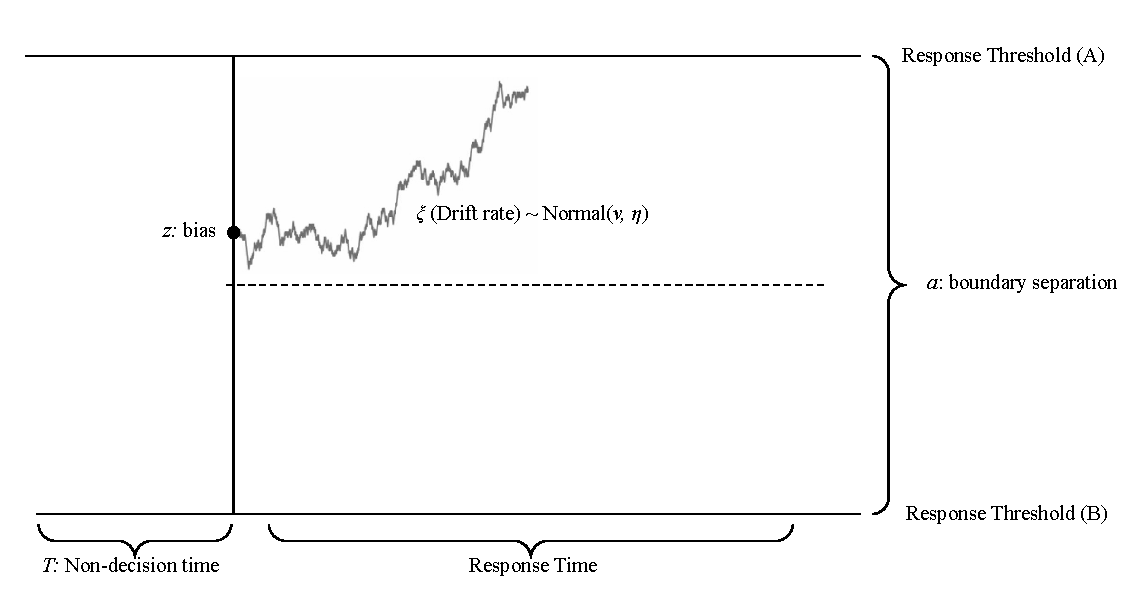
\includegraphics[width=\textwidth]{figure/ddm_model_grey.pdf}
  \caption{Simplified illustration of the drift-diffusion model. On every trial, after a period of time (T), an evidence accumulation process is initiated from the specified position (z) relative to the whole boundary separation (a). Evidence is gathered stochastically according to the drift rate ($\xi$) that follows a normal distribution with the mean v and the standard deviation $\eta$. When enough information is accumulated to cross one of the thresholds, a decision is made}
  \label{fig:diffusionmodel}
\end{figure}

Among five parameters shown in Figure \ref{fig:diffusionmodel} that govern the model's predictions, the starting point of information accumulation is the interest of this paper. The a priori bias of the participants can be defined as this starting position relative to decision thresholds, represented with \emph{z}, \emph{A}, and \emph{B} in Figure \ref{fig:diffusionmodel}. For example, suppose that the response bias (\emph{z}) is equal to half the distance between response thresholds (\emph{a/2}). In that case, we assume that participants do not have a bias towards either of the thresholds, and the decision to be made will be mainly determined by the drift rate \emph{$\xi$} --- the quality of stimuli's information. According to the model, as we increase the \emph{z} and hold the other parameters constant, we should see an overall increase in the number of A answers and a decrease in response times of A answers. On the other hand, if we decrease the \emph{z} with other parameters being constant, we expect an overall decrease in A answers and an increase in their response times.

An acceptability judgment task, a forced two-choice experiment, can also be conceptualized as a diffusion process. Possible answers, `acceptable' and unacceptable, can be represented as the upper and lower thresholds, respectively. \citeand{HammerlyEtAl2019}, building on \cites{Staub2009} work, proposed an implementation of the drift-diffusion model to the agreement attraction phenomenon and Marking and Morphing account. They hypothesized that as the response bias, starting position of the evidence accumulation, decreases, the acceptable responses to grammatical sentences should also decrease. Furthermore, this decrease should be sharper when there is a plural attractor due to its influence on the drift rate. Their argumentation follows from the Marking and Morphing account, where the agreement attraction effects surface due to the erroneous representation of the subject, and this representation is formed before the processing of the verb. Thus, the presence of a plural attractor should have the same effect in both grammatical and ungrammatical sentences.

On the other hand, in the cue-based retrieval model, the agreement attraction results from erroneous retrieval of the agreement controller when there is no single match to the cues provided by the verb. Thus, it should surface only in ungrammatical sentences, and the presence of the plural attractor should not influence the drift rates. When a participant's response bias changes, there should not be any effect of the plural attractor in grammatical sentences under the cue-based retrieval account of agreement attraction. These details are visualized in Figure \ref{fig:ddmSimulation}. 


\begin{knitrout}
\definecolor{shadecolor}{rgb}{0.969, 0.969, 0.969}\color{fgcolor}\begin{figure}[hbt!]

{\centering 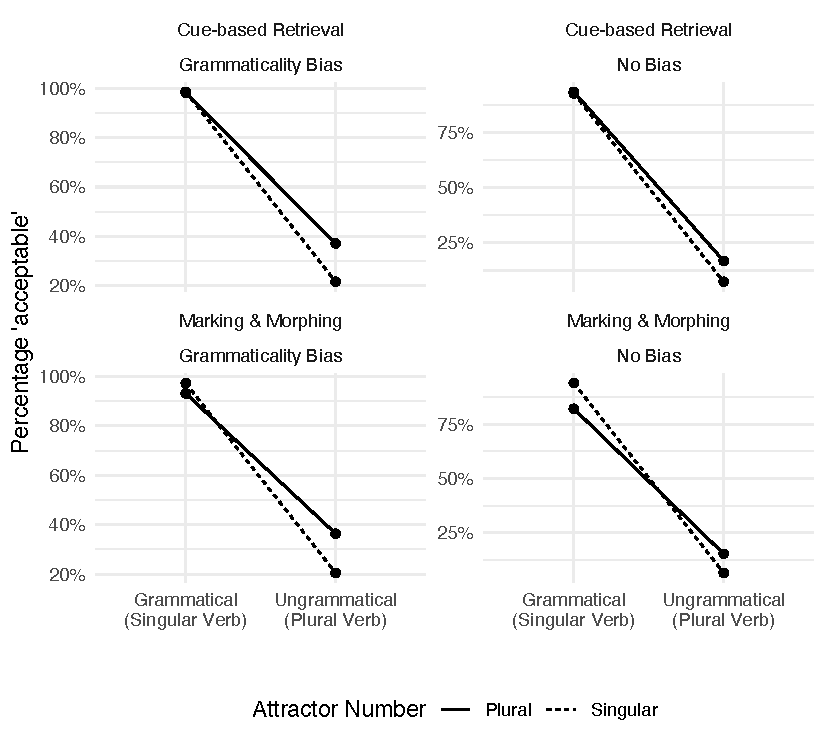
\includegraphics[width=\linewidth]{figure/ddmSimulation-1} 

}

\caption{Drift Diffusion Model predictions in which the drift rate is manipulated according to the assumptions of agreement attraction accounts along with a bias manipulation}\label{fig:ddmSimulation}
\end{figure}

\end{knitrout}


As it can be seen from Figure \ref{fig:ddmSimulation}, there is no effect of the plural attractor in grammatical sentences under the cue-based retrieval account in either bias condition. On the other hand, we see a clear difference in the influence of plural attractor depending on the bias manipulation under Marking and Morphing account. This difference follows from the fact that readers should first detect the ungrammaticality and only then consider the attractor as a candidate for the agreement under the cue-based retrieval account. In contrast, readers may be influenced by the plural attractor regardless of grammaticality under Marking and Morphing account.

When \cites{HammerlyEtAl2019} findings are compared to the visualization in Figure \ref{fig:ddmSimulation}, we see that their data is more compatible with Marking \& Morphing theories where the effect of sentence grammaticality is substantially reduced. Furthermore, the effect of the attractor number is roughly the same across the board. However, their manipulation of bias and results were only in English in a single experiment, which calls for a replication study in another language.

\section{Experiment 3}

In this chapter, we seek to clarify the status of the response bias in agreement attraction. We aim to replicate \cites{HammerlyEtAl2019} findings in another language, Turkish, with a different syntactic construction. To this end, we conducted a speeded acceptability judgment task with two within-subject manipulations (attractor number x verb number) and a between-subject manipulation (bias) which we introduced through instructions and the ratio of ungrammatical sentences as \citeand{HammerlyEtAl2019} did. We focus on number agreement attraction using an atypical structure, complex NP with a non-intervening genitive modifier. Both \citeand{LagoEtAl2019} and our Experiment 1 have established that these structures as in (\ref{ex:lago}) are prone to attraction effects.

\ea \label{ex:lago} 
  \gll {Milyoner-\{\O/ler\}-in} {terzi-si} tamamen gereksizce kov-ul-du-\{\O/lar\}.\\
  millionaire-\{\Sg/\Pl\}-\Gen{} tailor-\Poss{} completely without\_reason fire-\Pass-\Pst\{.\Tsg/-\Tpl\}\\
  \glt `The millionaire's/millionaires' tailor were fired\{\Sg/\Pl\} for no reason at all.'
\z

Considering our results in Experiments 1, 2A, and 2B, we conclude that agreement attraction effects in Turkish with an atypical syntactic structure are replicable. Building on this work, we sought to test the predictions of a drift-diffusion model and how the bias manipulation proposed by \citeand{HammerlyEtAl2019} would affect agreement attraction effects in grammatical sentences in Turkish. We reasoned that \cites{HammerlyEtAl2019} data, manipulation, and findings should be replicated, given that the Drift Diffusion model account of decision making is not limited to a particular language, a particular structure, or a particular demographic.



\subsection{Participants}

114 Turkish speakers participated in the experiment. All participants were recruited through Bo\u{g}azi\c{c}i University in exchange for course credit. Because 3 participants indicated that Turkish is not their first language, we excluded their data from the analysis. Participants had an average age of 20 (range: 29 - 18). The experiment was carried out following the principles of the Declaration of Helsinki and the regulations concerning research ethics at Bo\u{g}azi\c{c}i University. Before the experiment, all participants were explicitly asked for their consent and informed with respect to their rights. All sensitive information about the participants is anonymized.


\subsection{Materials}

In our study, we used the same experimental items that we used in our Experiment 1. 


In our experiment, all experimental sentences with a singular verb are grammatical, and all sentences with a plural verb are ungrammatical. Due to this distribution, we speculated that participants might form a strategy in which they automatically judge sentences ungrammatical when they see a plural ending. To this end, we created 60 filler items, half of which consist of ungrammatical sentences with singular marked verbs (\ref{ex:ungFiller}). In contrast, the other half is grammatical sentences with plural verbs (\ref{ex:grFiller}). 

Another purpose of the fillers was to manipulate participants' response bias. Along with the instructions, we have manipulated the number of grammatical and ungrammatical fillers in the experiments following \citeand{HammerlyEtAl2019}. We created two sub-experiments with two different ratio of ungrammatical stimulus. In the first sub-experiment, we intended to shift participants' bias towards ungrammatical responses by using only 10 grammatical fillers and 20 ungrammatical fillers. In the second sub-experiment, we wanted participants to have a bias towards grammatical responses. To ensure this, we used only 10 ungrammatical fillers and 20 grammatical fillers.

Most filler items started with a genitive-possessive NP similar to experimental items. However, this initial NP was not the subject of the main sentence but the subject of an embedded adverbial clause. In grammatical fillers (\ref{ex:grFiller}), we used a plural-marked verb whose subject is pro-dropped following the verb of the embedded adverbial clause. In ungrammatical fillers (\ref{ex:ungFiller}), we used a transitive verb whose non-local object lacked the case marking, making the sentence ungrammatical. While most of the fillers followed a strict template, 20 of the 60 were with no particular order, and half of them were grammatical sentences  with plural verbs (N=10) and the other half were ungrammatical sentences (N=10) with singular verbs. All of our experimental and filler items can be found in Appendix \ref{ap:exp3items}.


\ea \label{ex:fillers}
  \ea {Ungrammatical Filler} \label{ex:ungFiller}\\*
  \gll \"O\u{g}renci-nin hoca-s{\i} ayr{\i}l-{\i}nca proje birden unut-tu.\\
  student-\textsc{gen} teacher-\textsc{poss} leave-\textsc{when} project suddenly forget-\textsc{pst}\\
  \glt Intended: `Suddenly, he forgot the project when the student's professor left.'
  \ex {Grammatical Filler} \label{ex:grFiller}\\*
  \gll Patron-un yeme\u{g}-i yer-e d\"ok-\"ul-\"unce yeni-sin-i yap-t{\i}-lar.\\
  boss-\textsc{gen} meal-\textsc{poss} floor-\textsc{dat} spill-\textsc{pass}-\textsc{when} new-\textsc{poss}-\textsc{acc} do-\textsc{pst}-\textsc{pl}\\
  \glt `They prepared a new one when boss' meal spilled on the floor.'
  \z
\z





Before our experimental study, we ran a speeded acceptability judgment study where participants (N = 8) saw all experimental and filler items. Experimental items were distributed among four different lists according to a Latin Square design. One of the main reasons for conducting the norming study was to find the most acceptable grammatical and the least acceptable ungrammatical fillers for the Bias manipulation. We only used the ten least acceptable ungrammatical fillers to shift the response bias towards grammatical responses. Similarly, we only used the ten most acceptable grammatical fillers to shift the bias towards ungrammatical responses. We also wanted to check the overall acceptability of our grammatical items with singular attractor and confirm that there was no problem with the baseline sentences. We confirmed that our grammatical experimental items with singular attractor were found grammatical with no problem (M = 0.99, SE = 0.01). 

\subsection{Procedure}

The experiment was run online, using the web-based platform Ibex Farm \citep{Drummond2013}. Each experimental session took approximately 30 minutes to complete. After the first page participants landed, they were randomly assigned to one sub-experiment that incorporated the between-subject bias factor. Prior to the experiments, participants were asked to give informed consent to participate in the experiment. They then read the instructions, which included four already answered example sentences. After the instructions, they were given nine practice trials before the experiment began. After they finished practice trials, participants were prompted with a message stating the distribution of the sentences and asked to confirm that they understood the statement. The instructions are as follow:


\ea \label{ex:biasManip}
  \ea \label{ex:biasUngManip} {Ungrammaticality Bias Condition}\\*
  Bu deneydeki c\"umlelerin \c{C}O\u{G}U T\"urk\c{c}e kurallar{\i}na UYMAMAKTADIR!\\*
  `MAJORITY of sentences in this experiment DO NOT FOLLOW the rules of Turkish.'
  \ex \label{ex:biasGrManip} {Grammaticality Bias Condition}\\*
  Bu deneydeki c\"umlelerin \c{C}O\u{G}U T\"urk\c{c}e kurallar{\i}na UYMAKTADIR!\\*
  `MAJORITY of sentences in this experiment DO FOLLOW the rules of Turkish.'
  \z
\z

After participants were informed concerning the distribution of sentences' grammaticality, experiment was initiated in the IbexFarm. Each trial began with a blank screen for 600 ms, followed by a word-by-word RSVP presentation of the sentence in the center of the screen. Sentences were presented word-by-word in the center for the screen in 30 pt font size, at a rate of 400 ms per word. Participants saw a blank screen for 100 ms between each word, and to see the next item, they needed to press the space key. After every trial, participants are asked to indicate their acceptability judgment. The wording of the question is given in (\ref{ex:question}). 

\ea \label{ex:question}
Bu c\"umle kula\u{g}{\i}n{\i}za nas{\i}l geliyor? \\*
`How does this sentence sound to you?'
\z

The possible answers that participants could provide were either good or bad. Participants were asked to press the key P to indicate that a sentence is acceptable/good and Q to indicate that the sentence is unacceptable/bad. Within instructions before the experiments, they were told to provide judgments as soon as possible. If they did not respond within 5,000 ms during the experiment, the trial timed out, and participants were shown message `\emph{Please respond faster,}' in a red font.

Participants saw 40 experimental and 40 filler sentences. Experimental sentences were distributed among four different lists according to a Latin-square design. Every participant saw one version of the experiment with a specific list and one item per condition while seeing all filler items in that specific between-subject condition.


\subsection{Analysis}


The experimental data were collected from the IbexFarm website in a csv file format and imported to R for data cleaning, visualization, aggregation, and analysis. 

We excluded all 3 participants whose native language was not Turkish in the data cleaning process. Moreover, we removed the data for all participants who did not show sufficient sensitivity to the grammaticality in singular attractor conditions. Specifically, we excluded all participants whose difference in percentages of acceptable responses in grammatical sentences with singular attractors and ungrammatical sentences with singular attractors fell below 0.25 percentage points. Finally, we also excluded trials in which the participants missed the response deadline or gave too fast responses (below 200 ms). As a result, 9.05\% of trials were excluded from our experiment. 

% In Figure \ref{fig:MissingDataPlot}, you can see that the percentage of missing data or exclusion due to given RT and accuracy criteria compared to the total amount of data. Since the number of missing values and exclusions is quite small, we decided to ignore them and treat the data as missing completely at random. Due to this outcome, we treat them as they are irrelevant to the rest of the data.

% \begin{figure}[hbt!]
%   \centering
  
% <<MissingDataPlot,  echo=FALSE, fig.align='center', height=3, warning=FALSE,  dpi = 600, message=FALSE>>=

% missingdata_plot

% @
%   \caption{}
%   \label{fig:MissingDataPlot}
% \end{figure}




While reporting the aggregated details of the experimental data, we have used the categorical bias grouping we introduced following calculated bias values instead of our experimental manipulation. We calculated means and standard errors using tidyverse packages. In calculating the standard errors, we followed \citeand{Morey2008} and \citeand{Cousineau2005}. 


Since our research question is whether the change in bias affects acceptability in ungrammatical sentences and grammatical sentences, we grouped our responses according to the grammaticality of the sentences. We only use the ungrammatical sentences to see the already acknowledged agreement attraction effects. We then fitted another model, where we used only grammatical sentences to see the possible interaction between the plural attractor and the bias shift. We used the R packages brms \citep{R-brms_a,R-brms_b} and rstan \citep{R-rstan} to fit Bayesian hierarchical models \citep[e.g.,][]{GelmanHill:2007,NicenboimVasishth:2016}.

We fitted two Bayesian GLMs to yes responses as a function of the following predictors: (i) logarithm of the trial number (\emph{log}(trial)), (ii) sum-coded (0.5 vs. -0.5) attractor number (Pl.Attr.), (iii) continuous response bias value \emph{c} (Bias), along with two-way interaction of Pl.Attr. and Bias. We assumed that acceptable responses are distributed following a Bernoulli distribution with a probit-link function. We included only the experimental sentences in our analysis. Our models included maximal random-effect structures to the extent that our design justified. It allowed predictors in interest to vary by-participant (Pl.Attr., Bias) and by-item (Pl.Attr., Trial). The same priors from Experiment 1 is also used in these models. Our first model included only ungramatical sentences, while the second one included only grammatical sentences. Apart from this difference, all model specifications were the same.

\subsection{Bias Calculation} \label{sec:bias}

Before further statistical analysis, we wanted to test whether or not our bias manipulation was successful. Therefore, we calculated response bias value \emph{c} by participant, using equation (\ref{eq:bias}) \citep{MacmillanCreelman2005}. 

\begin{equation} \label{eq:bias}
c = -\frac{Z(Hit{\ }Rate)+Z(False{\ }Alarm{\ }Rate)}{2}
\end{equation}

Unlike \citeand{HammerlyEtAl2019}, we used only filler sentences in our response bias calculation. The reason for using only fillers is that we wanted to calculate response bias independently of the agreement attraction patterns. Since experimental items may be affected by either a grammaticality illusion or an ungrammaticality illusion, we believe using experimental items would create confounded results.

Figure \ref{fig:OurBiasBFPlot} shows the average bias value of participants in our experiment. We calculated the response bias using both only experimental items (\cites{HammerlyEtAl2019} way) and only filler items. On the x-axis, we indicate our manual bias manipulation, which also shown with different line types. As shown in Figure \ref{fig:OurBiasBFPlot}, our bias manipulation was not successful. The calculation using experimental items shows that there is a bias difference however it is reverse of what we originally intended. The calculation using filler items shows that both distributions heavily overlap and there is no difference in terms of participants' bias. We expected a significant bias towards grammatical responses (negative \emph{c}) in the grammaticality bias condition (Towards Yes). We also expected substantially more positive response bias values in the ungrammaticality bias condition. 


\begin{knitrout}
\definecolor{shadecolor}{rgb}{0.969, 0.969, 0.969}\color{fgcolor}\begin{figure}[hbt!]

{\centering 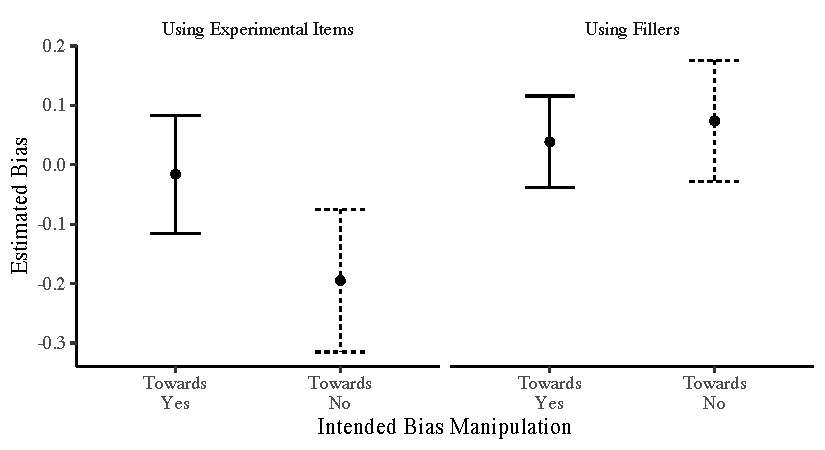
\includegraphics[width=\linewidth]{figure/OurBiasBFPlot-1} 

}

\caption{The average bias value in our Experiment 3 as a function of our intended bias manipulation and different calculation methods. The error bars indicate 95\% credible intervals. The negative \emph{c} values indicates a bias towards yes responses. The estimates in the left sub-figure are calculated with the experimental items only, while the estimates in the right sub-figure with filler items}\label{fig:OurBiasBFPlot}
\end{figure}

\end{knitrout}

We also calculated the Bayes Factor in favor of the hypothesis of no difference between grammaticality and ungrammaticality bias conditions using the statsExpressions package \citep{statsExpressions}. We deployed a one-sided Bayesian hypothesis test with an uninformative JZS Cauchy prior with the scale parameter $1.41$, which is specified by the statsExpressions package. It revealed that given the data, the null hypothesis (no difference) is eight times more likely (moderate evidence) than the alternative hypothesis of a significant difference between grammaticality and ungrammaticality response bias manipulation (BF$_{01}$ = 8, $\delta_{difference}^{posterior}$ = 0.03, CI$_{95\%}^{HDI}$ = [-0.09, 0.16], $r_{cauchy}^{JZS}$ = 1.41).

Given the distribution of our participants and the BF score, it is clear that participants did not respond to our bias manipulation.
We would expect to find at least moderate evidence towards the alternative model if our manipulation were successful. Graphically speaking, we would expect most of the subject points in the grammaticality bias condition to reside in the negative values, which was not the case.

In addition to our own results, we also computed the bias value of \cites{HammerlyEtAl2019} experiments using only the fillers for better comparison. In Figure \ref{fig:HammerlyBias}, we present the participants' estimated response bias following their method of calculating bias (through experimental items alone) as well as ours (through filler items alone). 


\begin{knitrout}
\definecolor{shadecolor}{rgb}{0.969, 0.969, 0.969}\color{fgcolor}\begin{figure}[hbt!]

{\centering 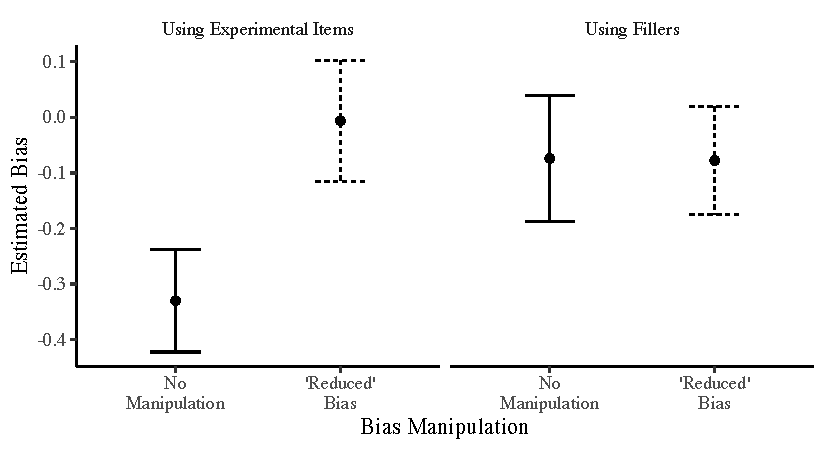
\includegraphics[width=\linewidth]{figure/HammerlyBias-1} 

}

\caption{The average bias value in \cites{HammerlyEtAl2019} study as a function of our intended bias manipulation and different calculation methods. The error bars indicate 95\% credible intervals. The negative \emph{c} values indicates a bias towards yes responses. The estimates in the left sub-figure are calculated with the experimental items only, while the estimates in the right sub-figure with filler items}\label{fig:HammerlyBias}
\end{figure}

\end{knitrout}
%Box plot of by-experiment response bias estimates with individual subject points from \cites{HammerlyEtAl2019} study. Box plots show the median value and first and third quartiles. Negative response bias signals a bias towards grammatical responses, while positive values mean a bias towards ungrammatical responses. The estimates in the sub-figure A are calculated with the experimental items only, while the estimates in the sub-figure B with filler items.

In their work, \citeand{HammerlyEtAl2019} state that they were able to manipulate the response bias between their experiments. 
We replicated their calculation and summary of response bias in the left-side of Figure \ref{fig:HammerlyBias} using experimental items. 
Our Bayesian hypothesis test suggests that given the data, the alternative hypothesis of a significant difference between grammaticality and ungrammaticality response bias manipulation is 1053 times more likely (extreme evidence) than the null hypothesis of no difference (BF$_{01}$ = 1/1053, $\delta_{difference}^{posterior}$ = 0.31, CI$_{95\%}^{HDI}$ = [0.18, 0.46], $r_{cauchy}^{JZS}$ = 1.41).

However, we argued that experimental items should not be included in the calculation of the response bias.
When only experimental items are used, the hit rate corresponds to the mean accuracy of grammatical conditions, including grammatical sentences with plural attractors. 
This means if there is an effect of a plural attractor in the grammatical conditions due to possible agreement attraction effects, let us say decreased accuracy, the response bias value will also be affected.
Similarly, the false alarm rate calculation will also be affected by the agreement attraction effect assuming that participants exhibit classic agreement attraction effects in ungrammatical sentences.
%Moreover, regardless of the item type, be it experimental or filler, participants' response bias should be reflected in their proportion of correct answers. 
For these reasons, we believe that their reported response bias summary using experimental items does not reflect the response bias truthfully and is affected by the agreement attraction effects present in their results.

When we use a calculation method that is not confounded with the agreement attraction effects, as in the right-side of Figure \ref{fig:HammerlyBias}, we see that the bias distribution among participants changes substantially, and there is no longer a significant difference between groups. 
Given the data, the null hypothesis of no difference between grammaticality and ungrammaticality response bias manipulation is eight times more likely (moderate evidence) than the alternative hypothesis of significant difference (BF$_{01}$ = 8, $\delta_{difference}^{posterior}$ = -0.00378, CI$_{95\%}^{HDI}$ = [-0.14, 0.14], $r_{cauchy}^{JZS}$ = 1.41).

Focusing only on the bias distribution based on the filler items, 
we see that participants were not responsive to the bias manipulation implemented by the researchers 
both in \cites{HammerlyEtAl2019} study and our study. 
Since \cites{HammerlyEtAl2019} findings were reliant on the fact that they manipulated the response bias, and participants' exhibited ungrammaticality illusions only with the change of the response bias, 
our re-evaluation of the response bias calculation cast a shadow on their findings and claims on the processing of agreement attraction. 
However, we were still able to test the theoretical claims of \citeand{HammerlyEtAl2019}: participants are biased towards grammatical responses, and as participants' response bias is shifted towards ungrammatical responses, they exhibit ungrammaticality illusions, i.e. an affect of plural attractor in grammatical sentences. 
To test this claim, we divided participants into two groups according to their calculated bias value \emph{c}. 
If the \emph{c} value is negative, we classified those participants as biased towards grammatical answers. 
If it was positive, they were treated as biased towards ungrammatical answers. 
We also included the continuous bias value for each participant to our Bayesian GLMs in all subsequent analyses.


%But we have very limited number of ungrammatical fillers. what if we also include singular attractor items in bias manipulatio as well?




\subsection{Results}

In this section, we provide summaries of the coefficient posterior distributions. We ran 4 chains with 1000 warm-up iterations and 4000 sampling iterations for our models. Our results report the posterior probability of the effect of coefficient $\beta$ being outside of the ROPE region, either smaller than $-0.1$ (\emph{P}($\beta < -0.1$)) or bigger than $0.1$ (\emph{P}($\beta > 0.1$)). If a distribution is completely outside of this area, we can say that we have definitive evidence for an effect. If it covers the practical equivalence area, we can say that according to our data, there seems to be no evidence for an effect. On occasions in which only a part of the distribution resides in the area, we explicitly quantify our degree of belief towards an effect. 



Accuracy in our fillers was relatively high with an average of 0.81 and standard error of 0.02 in participants with grammaticality bias and 0.81 and a standard error of 0.01 in participants with ungrammaticality bias. In Figure \ref{fig:FillerAverage}, we can see the individual means and standard errors according to the experimental conditions {bias} (on the x-axis) and {Grammaticality} (as a line type).


\begin{knitrout}
\definecolor{shadecolor}{rgb}{0.969, 0.969, 0.969}\color{fgcolor}\begin{figure}[hbt!]

{\centering 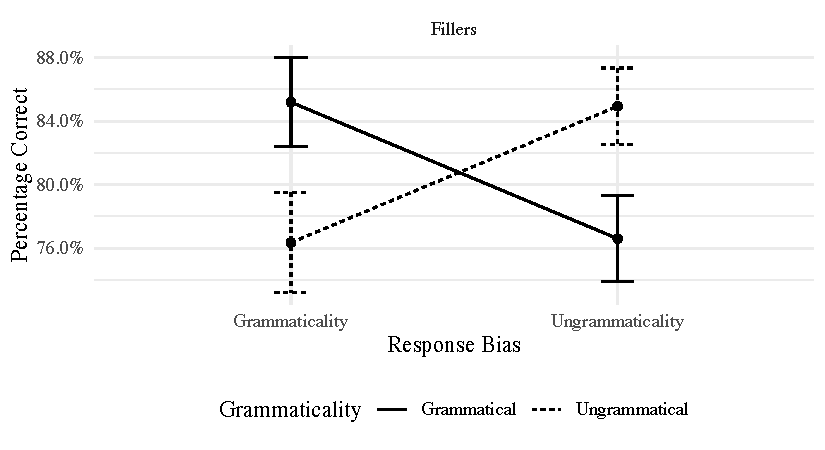
\includegraphics[width=\linewidth]{figure/FillerAverage-1} 

}

\caption{The average accuracy of fillers in Experiment 3}\label{fig:FillerAverage}
\end{figure}

\end{knitrout}
%The average accuracy of fillers in our study. Error bars signal standard errors calculated following \citet{Morey2008} and \citet{Cousineau2005}.


Figure \ref{fig:AvgResponse} shows the average proportions of acceptable responses in each of the eight conditions. Since we are interested in how bias affects the difference in acceptability between grammatical and ungrammatical sentences and the plural attractor interacts with this difference, we grouped the averages into facets according to the grammaticality of the sentences. While the x-axis shows the categorical bias grouping, which we introduced following calculated bias values, the line type shows the attractor number. We see that, on average, participants gave more acceptable responses in ungrammatical sentences with ungrammaticality bias (M = 0.08, SE = 0.01) rather than grammaticality bias (M = 0.2, SE = 0.02). More importantly for us, participants with ungrammaticality bias make more errors in grammatical sentences with plural attractors (M = 0.88, SE = 0.02) compared to the ones with singular attractors (M = 0.93, SE = 0.01). This effect of attractor number is not present in grammatical sentences when the participants have a grammaticality bias.


\begin{knitrout}
\definecolor{shadecolor}{rgb}{0.969, 0.969, 0.969}\color{fgcolor}\begin{figure}[hbt!]

{\centering 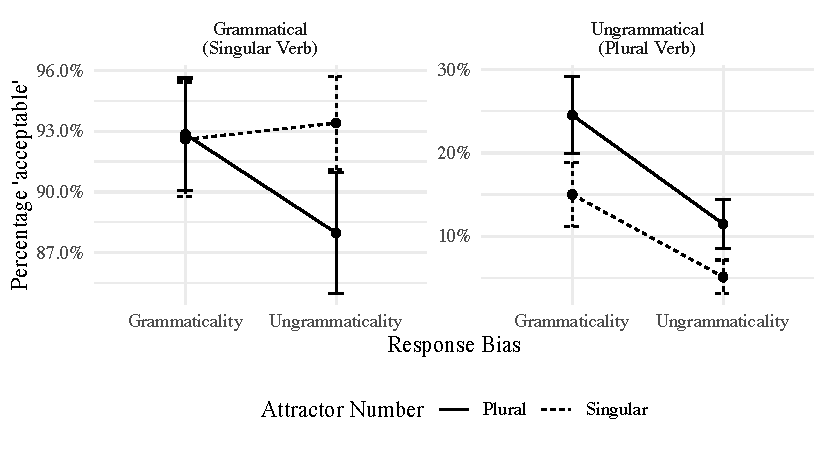
\includegraphics[width=\linewidth]{figure/AvgResponse-1} 

}

\caption{The average percentage of acceptable responses according to the experimental conditions in Experiment 3}\label{fig:AvgResponse}
\end{figure}

\end{knitrout}
%The average percentage of acceptable responses according to the experimental conditions in our study. Error bars signal standard errors calculated following \citet{Morey2008} and \citet{Cousineau2005}.

In Figure \ref{fig:UngramaticalBayesianGLM}, we see the posterior probabilities for our Bayesian GLM model with a probit link, in which we only use ungrammatical sentences. The negative main effect of ungrammaticality bias ($\hat{\beta}=-1.14;$ $CI=[-1.67; -0.61];$ $P(\beta>0.1)< .001$) indicates that, on average, participants gave less acceptable responses as their bias (calculated through fillers) shifted towards ungrammaticality. This verified that our bias calculation using fillers was effecting given that the effect is also present in experimental items. Additionally, the positive main effect of the plural attractor ($\hat{\beta}=0.47;$ $CI=[0.26; 0.70];$ $P(\beta>0.1)> .999$) is also significant, that is participants gave acceptable responses more often when the attractor is plural with an average response bias. The main effect of the trial no ($\hat{\beta}=-0.01;$ $CI=[-0.14; 0.12];$ $P(\beta>0.1)   .06$) show that it the order participants saw the experimental data did not affected the number of acceptable responses. Posterior probabilities suggested substantial evidence for the interaction between the ungrammaticality bias and the plural attractor ($\hat{\beta}=-0.47;$ $CI=[-1.09; 0.17];$ $P(\beta< -0.1)=    .87$), meaning that the effect of plural attractors was amplified when participants had an ungrammaticality bias.


\begin{knitrout}
\definecolor{shadecolor}{rgb}{0.969, 0.969, 0.969}\color{fgcolor}\begin{figure}[hbt!]

{\centering 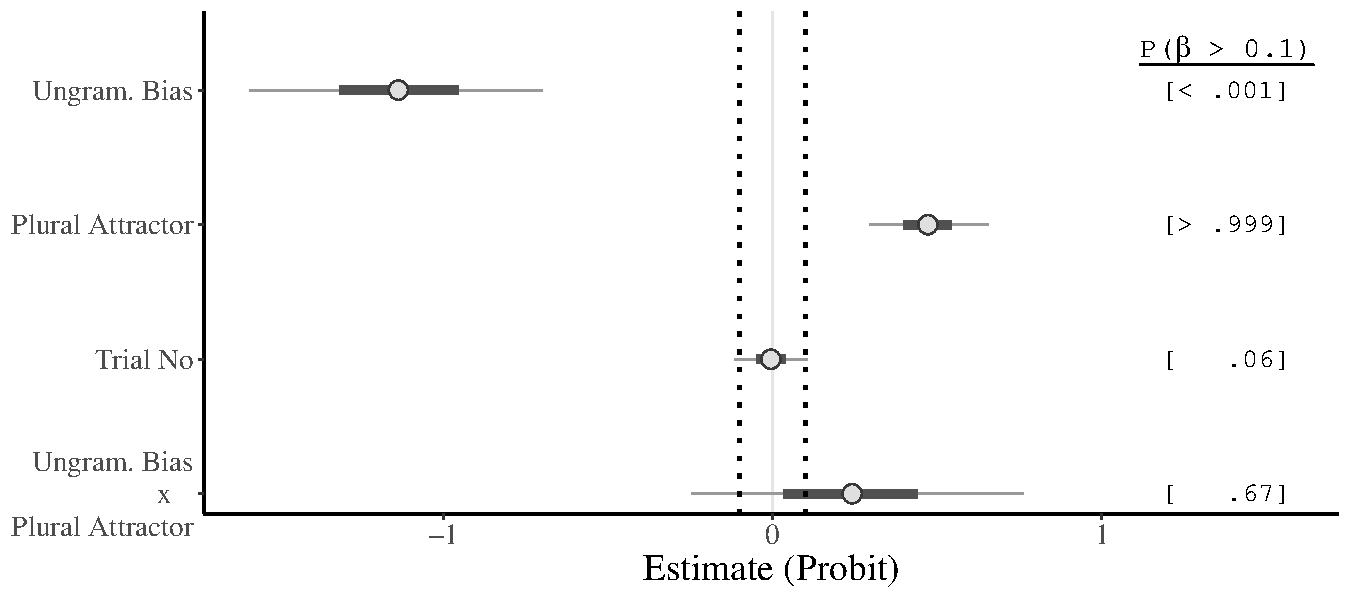
\includegraphics[width=\linewidth]{figure/UngramaticalBayesianGLM-1} 

}

\caption{Estimates and 95\% credible intervals for the probit regression coefficients for the model of responses to ungrammatical sentences in our Experiment 3}\label{fig:UngramaticalBayesianGLM}
\end{figure}

\end{knitrout}


Figure \ref{fig:GrammaticalBayesianGLM} shows the posterior distributions of a Bayesian GLM with grammatical sentences alone. The main effect of ungrammaticality bias ($\hat{\beta}=-0.24;$ $CI=[-0.79; 0.31];$ $P(\beta< -0.1)=    .69$) was relatively weak, meaning that we cannot definitively say participants found grammatical sentences more acceptable as their bias is shifted towards ungrammatical answers. This effect, again, verified that our bias calculation was on the right track. 

Meanwhile, the main effect of the plural attractor in grammatical sentences ($\hat{\beta}=-0.22;$ $CI=[-0.51; 0.04];$ $P(\beta< -0.1)=    .82$) tells us that with an average response bias, participants give less acceptable responses with a substantially higher probability when a plural attractor is present. Given that the average bias in our experiment is 0.06, which corresponds to a neutralized grammaticality bias, we can say that the apparent main effect of the plural attractor is an indicator of agreement attraction effects in grammatical sentences. Moreover, the negative interaction between the ungrammaticality bias and the presence of a plural attractor ($\hat{\beta}=-0.47;$ $CI=[-1.09; 0.17];$ $P(\beta< -0.1)=    .87$) tells us that participants with an ungrammaticality bias are even more affected by the presence of a plural attractor in grammatical sentences. 

\begin{knitrout}
\definecolor{shadecolor}{rgb}{0.969, 0.969, 0.969}\color{fgcolor}\begin{figure}[hbt!]

{\centering 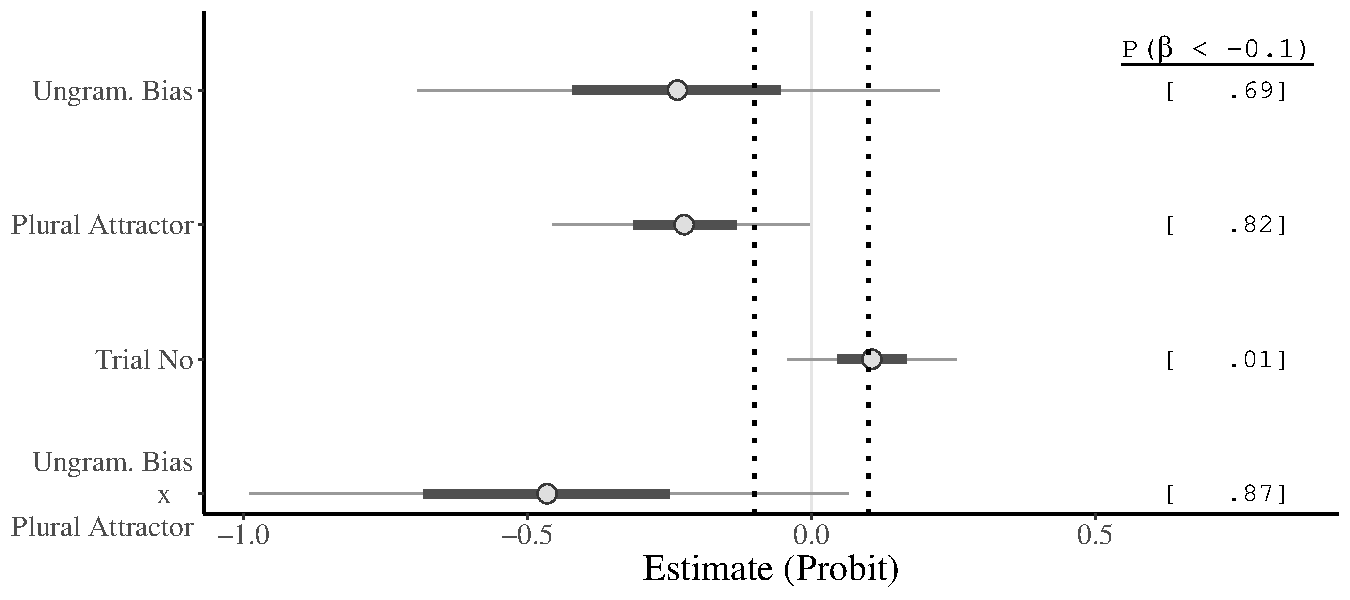
\includegraphics[width=\linewidth]{figure/GrammaticalBayesianGLM-1} 

}

\caption{Estimates and 95\% credible intervals for the probit regression coefficients for the model of responses to grammatical sentences in our Experiment 3}\label{fig:GrammaticalBayesianGLM}
\end{figure}

\end{knitrout}

Taken together, our results suggested that the bias shift towards ungrammatical responses, which we calculated using the filler items, reduced overall acceptable responses in ungrammatical experimental items as expected in the drift-diffusion model. In addition, we have moderate evidence that tells us that ungrammaticality bias affects acceptable responses in grammatical sentences. With an average bias, the probability of giving acceptable responses is reduced substantially with plural attractors in grammatical sentences compared to sentences with singular attractors in grammatical sentencens, creating an ungrammaticality illusion. However, we can say that the effect of the plural attractor is more pronounced in people with ungrammaticality bias in grammatical sentences than in ungrammatical sentences. This emphasizes that the ungrammaticality illusion that we observe in grammatical sentences with plural attractors is amplified in a continuous manner as bias shifts towards more and more ungrammatical responses as expected by the drift-diffusion model.

\section{Discussion}

This chapter re-examined \cites{HammerlyEtAl2019} findings. It also tested the predictions of the drift-diffusion model in agreement attraction: an amplified effect of plural attractor in grammatical sentences with a decreased bias towards grammatical responses. 
Suppose readers are biased to find sentences grammatical more often than ungrammatical, and lack of agreement attraction effects in grammatical sentences is due to this fact. 
In that case, they should be making more errors in grammatical sentences with plural attractors when their bias towards grammatical responses is neutralized or reversed. 

To this end, we conducted a speeded acceptability judgment experiment (N=114) with two within-subject factors (Attractor number x Verb number: 2x2) and a between-subject factor Bias. 
Following \citeand{HammerlyEtAl2019}, we manipulated the response bias utilizing instructions and the ratio of ungrammatical fillers. 
Our results can be summarized as follows. 
Our participants did not respond to the bias manipulation uniformly, and the effect of the instructions and the ratio of ungrammatical sentences was not significant. 
When we calculated the response bias following \citeand{MacmillanCreelman2005} and used it in our Bayesian GLM as a continuous predictor, 
we saw that the presence of a plural attractor substantially reduced the acceptable responses in grammatical responses as well.  
This effect of the plural attractor was even more amplified when the participants had a bias towards ungrammatical answers.

Based on the participants' response profile and our simulation results, we can say that our findings were parallel with those of previous studies that showed processing difficulty in grammatical sentences with plural attractors as differences in response times or acceptable responses.
Furthermore, our results show that attraction in grammatical sentences may emerge as a difference in acceptable responses, following from accounts of attraction that rely on feature percolation and faulty encoding of subjects \citep[][among others]{EberhardEtAl2005}.

These findings present a challenge for retrieval accounts \citep{LagoEtAl2015, LagoEtAl2019, WagersEtAl:2009}, which argue that for participants, the plurality of the attractor is only relevant in ungrammatical sentences, which is only when they may consider other DPs as a possible controller. 
Since attractor, be it single or plural, does not come into play unless the sentence is ungrammatical, these accounts predict that participants' bias should not affect the acceptability in grammatical sentences. 
Thus, the lack of a significant interaction between the grammaticality and the plural attractor in most studies suggested that retrieval accounts may capture agreement attraction effects better (Schlueter, Parker, \& Lagu, 2019; Hammerly et al., 2019; Lago et al., 2021). 

However, when bias is accounted for, it seems that grammaticality asymmetry is not due to the nature of how subject-verb dependency is processed as argued before by the retrieval accounts \citep[][among others]{WagersEtAl:2009}, but a direct residue of how participants make decisions in forced-choice experiments. 

What is still left as an intriguing issue is that neither \citeand{HammerlyEtAl2019} nor we could introduce a bias manipulation according to the response bias values calculated through filler items. Despite this fact, their results from Experiment 3 exhibit an apparent effect of plural attractor in grammatical and ungrammatical sentences. These results would be expected only if their bias manipulation were successful.

To sum up, we attempted to replicate \cites{HammerlyEtAl2019} study in Turkish with a different syntactic construction: a noun phrase with a genitive modifier. We argued that response bias shift might result in ungrammaticality illusion in another language with a structure that was found to be attraction-vulnerable \citep{LagoEtAl2015}. We presented our speeded acceptability judgment task results which showed comparable results with \citeand{HammerlyEtAl2019}. While we could not manipulate participants' response bias, we replicated the theoretical claims of \citeand{HammerlyEtAl2019}. We confirmed the predictions of the Marking \& Morphing account implemented with the drift-diffusion model. We argue that cue-based retrieval models cannot account for the role of the response bias in agreement attraction, which we demonstrated. 


\chapter{DISCUSSION} \label{ch:discussion}

This thesis set out to understand the processing errors in the subject-verb dependencies in Turkish. The focus has been to clarify the agreement attraction effects in Turkish and eliminate possible confounds in the existing literature. We wanted to understand what aspects of agreement attraction findings could be explained with extra-linguistic phenomena like storing erroneous parses, using form heuristics, or having a response biases. To this end, we determined three possible confounds to test:

\begin{enumerate}[label=(\roman*)]
    \item {A lingering effect of an erroneous parse due to case syncretism:} Local ambiguity due to a case syncretism between a subject compatible marking and a non-compatible marking on the subject head may lead participants to retrieve the attractor as an agreement controller.
    \item {A task-specific response strategy using form heuristics:} Unlike other languages, Turkish plural marker on nouns and the plural agreement marker on verbs are homophones. Assuming participants engage in shallow processing, they may form a strategy where they answer questions by matching the final plural agreement with a previous plural marking in the sentence.
    \item {Response bias as an underlying cause of existing effects:} Patterns of agreement attraction in yes percentages might be due to participants' a priori tendency to give yes responses. \citeand{HammerlyEtAl2019} showed the true nature of agreement attraction by getting rid of this existing response bias. Turkish agreement attraction might also be affected by the presence of an underlying response bias.
\end{enumerate}

To test these interactions between the aforementioned phenomena and agreement attraction, we conducted three speeded acceptability judgments. Section \ref{ch6predictions} puts forward the predictions of the cue-based retrieval and the Marking and Morphing acconts of agreement attractions. Section \ref{ch6summary} summarizes our findings in these experiments in broad strokes. Sections \ref{ch6case}, \ref{ch6form}, and \ref{ch6bias} will discuss the implications of these experiments. In Section \ref{ch6syntax}, we firstly discuss how two syntactic theories of sentence object relative clauses predict contrasting patterns in the Marking and Morphing account of attraction. We then, discuss a possible confound we have not covered in this thesis: the possibility of honorific reading in Turkish agreement attraction effects in Section \ref{ch6hon}.


\section{Predictions} \label{ch6predictions}

Before summarizing our findings, we would like to lay out the predictions of the two most important accounts of agreement attraction.

\subsection{Experiment 1}
In our first experiment, we manipulated the overt-case marking of the subject head. 

\subsubsection{Cue-based retrieval account}

In the cue-based retrieval account, the comprehension process in language utilizes a structured search to satisfy dependencies. Certain elements, such as verbs, trigger a search by providing specific cues, such as [+{pl}]. The dependency is satisfied when there is a match between the cues provided by the verbs and the features from the previous chunks. Attraction occurs when multiple chunks are considered for possible retrieval. 

The exact information stored in the chunks and the same cues utilized in this process is still an open debate \citep{ArnettWagers:2017}. Morphological realization of the abstract case may also be another feature stored in the chunk and be used as a cue in the retrieval process, as recent studies on Russian indicates \citep{SlioussarMalko2016, Slioussar2018}.

Thus, we believe that the cue-based retrieval account would expect reduced attraction effects when the case on the subject head is not ambiguous. 

\subsubsection{Marking and morphing account}

In the Marking and Morphing account, the attraction occurs due to the probabilistic spread of the plurality from the attractor to the root node of the subject. This spread activation depends on the number information of every phrase within the subject and their syntactic distance to the root node. 

Due to the nature of the activation spread, the Marking and Morphing account would not predict any additional interference due to the case-related manipulation. 

\subsection{Experiments 2A \& 2B}
In experiments 2A and 2B, we tested the interaction between the form-advantage and agreement attraction. We utilized the homophony between nominal plural marking and verbal plural agreement in Turkish. 

\subsubsection{Cue-based retrieval account}
We argued that if participants utilize form-related features rather than abstract features, we should also observe attraction effects with verbal attractors. 

Many implementations of the cue-based retrieval account do not specify any cue for the category of the agreement controller or the category of the stem of the agreement controller. Since Turkish reduced object relative clauses may also serve as agreement controllers, we believe the cue-based retrieval account would predict a presence of an attraction effect in ungrammatical sentences. 

\subsubsection{Marking and morphing account}

Following the intricacies of the spreading activation formula, we believe that the Marking and Morphing would also expect a presence of an attraction effect in ungrammatical sentences. However, since the syntactic position of the verbal plural agreement is embedded more deeply, we expected either significantly decreased attraction effects or a lack of its presence due to our experimental choices.   

\subsection{Experiment 3}
In experiment 3, we tested whether manipulating a priori response bias impacts the effect of attractor number in grammatical sentences. 

\subsubsection{Cue-based retrieval account}
Under the assumptions of the cue-based retrieval account, changing a priori bias would not result in an amplified effect of attractor number in grammatical sentences. This lack of increase is because attraction is expected to surface only in cases with more than a single match. In grammatical sentences, the dependency between the verb and the subject is satisfied without any problem. The number and the subjecthood features, such as case and syntactic position, fully match the cues provided by the verb in grammatical sentences. Thus, no other candidate for the agreement controller role should be entertained.


This understanding of attraction effects necessitates that the grammaticality asymmetry is due to the characteristics of sentence processing. Given the assumptions of this model, we believe that the cue-based retrieval account would expect no attraction effects when the a priori response bias is manipulated. 

\subsubsection{Marking and morphing account}

A priori response bias of the participants is not implemented directly in the Marking and Morphing account. As far as we know, this account is not equipped to integrate response bias into the attraction phenomenon. 

However, unlike the cue-based retrieval account, The Marking and Morphing account does not expect a grammaticality asymmetry: the effect of plural attractor should be comparable in grammatical and ungrammatical sentences. While this asymmetry is a direct result of the sentence processing mechanisms in the cue-based retrieval phenomenon and is intertwined with the attraction process, the Marking and Morphing account is agnostic to this phenomenon.  

A recent study by \citeand{HammerlyEtAl2019} showed that this asymmetry is related to the nature of linguistic experimenting. They argue that participants have a general tendency to answer yes more often than no. They utilized \cites{Ratcliff1978} Drift Diffusion Model and showed that when the extra-linguistic factor bias is controlled, the predictions of the Marking and Morphing account hold.

We reasoned that \cites{HammerlyEtAl2019} data, manipulation, and findings should be replicated, given that the Drift Diffusion model account of decision making is not limited to a particular language, a particular structure, or a particular demographic. That is, participants with no a priori bias towards yes responses should also exhibit attraction effects in grammatical sentences.


\section{Summary of findings} \label{ch6summary}
Experiment 1 was concerned with the possible confound in \cites{LagoEtAl2019} study. They argued that Turkish native speakers accepted ungrammatical sentences with plural attractors more often than their singular attractor counterparts because the genitive case marking is usually used as a subject marker in Turkish. However, all sentences in their experiment had two possible parses until they encounter the matrix verb, which was the last element in the sentence. In one possible parse, participants formed a representation where the subject was a complex NP with a genitive-marked modifier. In the second possible parse, their representation included an embedded sentence with a genitive-marked subject and an accusative-marked object. We argued that the present agreement attraction effects might be due to this local ambiguity and lingering effects of not-completely abandoned parses. We disambiguated the subjects they used and aimed to replicate their findings. If the present effects were due to linguistic features, such as the [+{subj}] feature and did not result from an erroneous parse, we expected to find comparable results to \cites{LagoEtAl2019} findings. Given our data, our results contradicted our hypothesis and verified that case syncretism does not play a role in Turkish agreement attraction. 

Experiments 2A and 2B dealt with another possible hypothesis that might explain \cites{LagoEtAl2019} findings. Due to the unique feature of Turkish agreement attraction, we hypothesized that participants might use form-driven processing strategies, assuming that they engage in shallow processing. Unlike other languages in which agreement attraction is tested, Turkish nominal and verbal plural markings are homophonous. One possible explanation of Turkish agreement attraction findings is that participants do not fully process sentences and match two \emph{-lar} markings in a sentence to judge the grammaticality of sentences when they do not have sufficient information. On some occasions where they could recall that there was a plural present but could not recollect the exact host of the plural marking, they might deem sentences acceptable. To test this hypothesis, we used plural marked verbs of reduced relative clauses as attractors and expected comparable effects of plural marking in ungrammatical sentences in Experiment 2A. However, our results contradicted our hypothesis: participants were highly successful in detecting ungrammatically in RC attractor conditions independent of the presence of a plural attractor. 

In Experiment 2B, we included four new conditions to test whether our findings in Experiment 2A were because that participants have no way of associating the previous plural marking with grammaticality. Since Turkish plural marking on the verb is not obligatory, participants may not have a priori tendency to match two \emph{-lar} markers in sentences. For priming participants to consider our hypothesized matching mechanism, we included new conditions in which we had a complex NP with a genitive-marked modifier like the ones we used in Experiment 1. With new conditions, we expected our participants to accept ungrammatical sentences with a plural verbal attractor more often than their singular verbal attractor counterparts. We, again, found that participants did not make any additional judgment errors when there was a plural verbal attractor. However, we also found that the overall acceptability of ungrammatical sentences with genitive-marked attractors reduced substantially compared to Experiment 1. Even though we were not able to confirm that participants utilized form heuristics to complete the task, our results suggest that the task and the other conditions might influence the magnitude of the agreement attraction effects.

In Experiment 3, we tested whether the nature of the task might influence the mainstream patterns of attraction. With the nature of a task, we refer to the instructions and the number of ungrammatical and grammatical fillers. Recently, \citeand{HammerlyEtAl2019} found that participants made judgment errors in grammatical sentences almost as often as they did in ungrammatical sentences. Following \cites{Ratcliff1978} DDM model, they argued that participants had a priori response bias towards yes responses, and when this bias was neutralized through the instructions and the ratio of ungrammatical sentences to grammatical sentences, the main effect of plural attractor would be present independent of sentence grammaticality. Their results verified this hypothesis and supported attraction accounts based on representational errors rather \citep{EberhardEtAl2005} than retrieval errors \citeand{WagersEtAl:2009}. We wanted to replicate these findings in Turkish with a different syntactic structure since both grammaticality asymmetry, and DDM accounts are not limited to a single language, and their results were only attested in one language: English. When we assessed the response bias using fillers, we found that we could not manipulate participants' response bias. However, we also found that \citeand{HammerlyEtAl2019} also could not manipulate response bias according to our calculation of response bias using fillers. Thus, we grouped our participants into two using calculated bias estimates and not the experimental manipulation. Our results, using this grouping, confirmed theoretically significant aspects of \citeand{HammerlyEtAl2019}: With neutralized bias, participants judged grammatical sentences as ungrammatical when there was a plural attractor present. 

\section{Case syncretism} \label{ch6case}

As discussed in Chapters \ref{ch:accounts} and \ref{ch:exp1}, we wanted to check the effects of case syncretism in Turkish agreement attraction. Even though previous research on case syncretism presents a solid case for affecting sentence processing, the literature on the agreement attraction was not coherent. Experiments in initial studies mostly included confounds such as attractor type \citep[][in Dutch]{HartsuikerEtAl2003} and syntactic position \citep[][in French]{FranckEtAl2006}. Later, studies were conducted on other languages in which researchers could manipulate the case syncretism or distinctive case marking without introducing confounds. However, these results were also not conclusive: while Eastern Armenian did not show any interaction between case syncretism and agreement attraction \citep{AvetisyanEtAl:2020}, results from German and Russian experiments showed that when participants saw attractors with a case marking that is syncretic between two cases, they make more agreement errors with plural attractors in the vicinity than with plural attractors that carry distinctively marked case.

However, all these studies manipulated the case syncretism on the attractor. We can infer from \citeand{BockEberhard93} and \citeand{HaskellMacDonald2003} that the effect of a manipulation changes depending on whether the attractor or the head is affected by the manipulation. Notionally plural nouns do not appear to play a role in agreement attraction when they were first introduced in the attractor position \citep{BockEberhard93}. However, \citeand{HaskellMacDonald2003} showed that the notional plurality of nouns has a tremendous effect when it is introduced in the head noun.

Additionally, the previous experiments on case syncretism never introduced a local ambiguity. Even though the case on the attractor was syncretic, this case syncretism never resulted in syntactic ambiguity. The syntactic relation between the attractor and the subject head was clear. In \cites{LagoEtAl2019} Turkish experiment, however, participants were able to entertain two different syntactic structures until they saw the last element in every item. In one possible parse, the first DP, the attractor, could be interpreted as a genitive-marked modifier of the second NP, the subject head. In another possible parse, participants might entertain a syntactic structure involving an embedded sentence when they see a genitive-marked DP. The first DP could then be interpreted as the subject of an embedded sentence, while the second DP could be interpreted as a direct object of the embedded sentence.  

Drawing parallelism from the line of work in the notional plurality issue, a case syncretism between a non-subjecthood case and a subjecthood case might have played an important role in Turkish agreement attraction effects. Considering that the case syncretism introduces a local ambiguity, we hypothesized that the present agreement attraction effects in \cites{LagoEtAl2019} work might decrease or disappear when we disambiguated the case syncretism and used distinctively marked case on the head.

We saw that Turkish agreement attraction effects were not contingent on the local ambiguity and case syncretism. When we disambiguated the subject marking on the head, our results were comparable to \cites{LagoEtAl2019} findings. In both studies, there was an interaction between the presence of a plural attractor and grammaticality. Participants accepted ungrammatical sentences with plural attractors more often than the ones with singular attractors, and this effect was not present in grammatical sentences. 

Our results contradicted our hypothesis that lingering effects of an erroneous parse might affect the acceptability of the sentence. Either participants do not entertain the syntactic parse involving an embedded structure due to its being less economical to do so, or they quickly recover from the local ambiguity so that it does not affect the grammaticality judgment. Our experiment was not equipped to answer this question; however, a future study involving a self-paced reading experiment or an eye-tracking experiment might answer this question.

\section{Form heuristics} \label{ch6form}

Experiments 2A and 2B tested whether participants use form heuristics to complete the grammaticality judgment task. Chapters \ref{ch:accounts} and \ref{ch:exp2} discussed the potential reasons for us to entertain an alternative hypothesis for present agreement attraction effects in Turkish. Namely, participants may use a strategy based on matching \emph{-lar} morphemes when they could not judge the sentence reliably due to memory uncertainty. 

We compared sentences containing a reduced relative clause with an overt plural marking to sentences containing a genitive marked subject modifier to test this hypothesis. If participants used the form of \emph{-lar} markings to answer grammaticality judgments, we expected comparable effects in ungrammatical conditions with verbal attractors as well.

However, our results suggested that participants do not use form heuristics in Turkish agreement attraction effects. We could not find an effect of plural attractors in ungrammatical sentences within verbal attractor conditions. This finding was verified with an additional experiment, where we included minimally different genitive marked subject modifier conditions to the experiment. We took the lack of an effect in both experiments to indicate that participants did not use forms as a cue in the processing of subject-verb dependency and that the part of speech tag of the attractor was important even when the attractor was a nominalized relative clause.

On the other hand, our results showed a reduced magnitude of agreement attraction in genitive marked subject modifier conditions when the experiment included verbal attractor conditions. Even if we could not find an evidence of a form-heuristics-based mechanism, we could interpret these findings as mild evidence of task effects. The presence of a set of clearly detectable grammatical and ungrammatical subject-verb dependency conditions (i.e., verbal attractor conditions) might have reduced overall errors in other conditions, which included a genitive marked subject modifiers as attractors. 

We also found a small positive effect of the presence of a plural attractor in grammatical sentences in Experiment 2A. This finding was unexpected given previous agreement attraction studies in which the presence of a plural attractor either affected the acceptability of grammatical sentences negatively or did not affect them. We believe that a plural marking on a reduced relative clause could induce an impersonal reading, whereas the lack of a plural marking would require a specific subject in the context \citep{Kornfilt:2011}. We believe that the positive effect of plural attractors in grammatical sentences might be due to this difference between interpretations. Unfortunately, our results in ungrammatical sentences might also be affected with this interpretation difference. The presence of a plural marker on the reduced relative clause might be too marked to go unnoticed since it might have an impersonal reading contribution. 

\section{Response bias} \label{ch6bias}

Experiment 3 re-examined \cites{HammerlyEtAl2019} hypothesis that the grammaticality asymmetry observed in the comprehension studies was due to the a priori response bias. The DDM model applied to the Marking and Morphing account of attraction predicts that as the tendency towards yes responses decreases, the effect of a plural attractor in grammatical sentences should increase. \citeand{HammerlyEtAl2019} found an increased effect of plural attractor in grammatical sentences in their Experiment 3, where they informed participants that most sentences are ungrammatical in the experiment. We argued that shifting response bias towards no responses might induce ungrammaticality illusion in addition to the grammaticality illusion in another language with a structure that was found to give rise to attraction effects \citep{LagoEtAl2019}.

To test this hypothesis, we have used experimental items from Experiment 1 and introduced a within-subject bias (bias towards grammaticality x bias towards ungrammaticality) manipulation using some instructions and the ratio of ungrammatical sentences to grammatical sentences. We only manipulated the number of ungrammatical fillers and grammatical fillers; the experimental items were the same in both within-subject conditions.

We calculated the participants' response bias using the formula provided in \citeand{MacmillanCreelman2005}. It seemed that we were not able to uniformly manipulate our participants' response bias; the the effect of instruction and the ratio of ungrammatical fillers did not create a systematic difference in participants' bias. However, when we included the calculated bias in our Bayesian GLM, we saw that the grammatical conditions with plural attractors were less likely to be judged as grammatical when participants did not have a bias toward yes responses. Our findings were parallel with \cites{HammerlyEtAl2019} findings and theoretical assumptions, even though we could not manipulate the bias properly. 

Both our and \cites{HammerlyEtAl2019} findings cannot be accounted for if we assume a cue-based retrieval account, which argues that the attractor's plurality is only relevant in ungrammatical sentences \citep{LagoEtAl2015, LagoEtAl2019, WagersEtAl:2009}. Since there would be a complete match in grammatical sentences between the cues provided by the singular verb and features in the singular subject head, a plural attractor has no way of interfering with the subject-verb dependency. Thus, the lack of an effect induced by plural attractors in grammatical sentences (grammaticality asymmetry) result from the internal mechanisms of how a cue-based retrieval system works. The response bias has no way to affect the retrieval process, and therefore, should not influence processing agreement attraction. 

The Marking and Morphing account, on the other hand, expects a comparable effect of plural attractor in both grammatical and ungrammatical sentences. According to this account, agreement attraction occurs after an erroneous representation is formed. Like grammaticality illusion, in which participants erroneously judge a grammatical sentence as an ungrammatical one, there should be an ungrammaticality illusion, which means that participants occasionally deeming grammatical sentences as ungrammatical. The non-existence of such an effect in the previous agreement attraction experiments can be explained via a response bias towards yes responses.

Even though both we and \citeand{HammerlyEtAl2019} could provide evidence for the representation-based attraction accounts, we believe that \cites{HammerlyEtAl2019} results should be verified. We used filler items to determine and check our participants' bias values. However, \citeand{HammerlyEtAl2019} used all items in their experiment. We believe that using all items might create a problematic picture since the bias calculation would also include agreement attraction effects in grammatical and ungrammatical sentences. If there is a bias towards any response type, it should also be present in fillers. When we checked participants' response bias in their Experiments 1 and 3 using their fillers, we saw that they could not manipulate their participants' bias systematically as well. Nevertheless, their Experiment 3 clearly shows an effect of a plural attractor independent of the sentence grammaticality, which might be due to their participant sample.

\section{Syntactic assumptions} \label{ch6syntax}

In Chapter \ref{ch:exp2}, we have discussed that our results from Experiment 2 might be due to syntactic depth differences. A number information coming from the verb of a relative clause, which is embedded in more phrases than the number information coming from a genitive modifier, could not induce attraction effects. The Marking \& Morphing account of agreement attraction predicts this effect of syntactic depth. In their spreading activation formula used to calculate the final number representation of a nominal phrase, the contribution of various elements in the same phrase is weighted according to their syntactic distance to the root node of the subject phrase.

Here, I repeat the structures we posited in Chapter \ref{ch:exp2}. The structure for a Genitive-Possessive DP shown in (\ref{syntax:genpossRepeat}) is adapted from \citeand{OzturkTaylan2016}. Prior to their study, many other researchers as well assumed a structure in which the genitive-marked DP starts from a position that is close to the head NP but moved up to the spec DP position to be marked with a genitive case \citep{Lewis70,Dede78, Kornfilt97, Kornfilt85,Ozsoy94, Yukseker98, Arslan2006, Arslan2009, Goksel2009}. Due to its position, the weight of the number information coming from the DP \emph{y\"oneticilerin} would be very high, and the additional number information would easily influence the final number representation.

\ea \label{syntax:genpossRepeat} {Genitive-Possessive DP}\\*
\scalebox{1}{\begin{forest}
%fned
    [DP
        [DP\\Y\"oneticilerin\textsubscript{i}]
        [DP
            [\emph{n}P
                [DP\\\emph{t}\textsubscript{i}]
                [\emph{n}P
                    [NP [N\\a\c{s}\c{c}{\i}]]
                    [\emph{n}\\-s{\i}]
                ]
            ]
            [D]
        ]
    ]
    % \path[fill=red] (.parent anchor) circle[radius=2pt];
    % \path[fill=red] (!1.child anchor) circle[radius=2pt];
\end{forest}}
\z

On the other hand, when we look at the inner syntax of a Turkish relative clause, there is yet to be a single representation that is widely assumed. The structure shown in \ref{syntax:orcRepeat} is adapted from \cites{Aygen2002} work. The relative clause is an adjunct at the DP level and consists of syntactic phrases VP, little \emph{v}P, TP, little \emph{n}P, and DP. It assumes that Turkish relative clauses are not full-CPs. This assumption follows from the fact that CP-level adverbials like \emph{Allah'tan} (\emph{Thank God}) cannot be licensed in relative clauses \citep{Goksu2018, Aygen2002}. We also assume that terminal nodes introduce full words with feature specifications and not morphemes, following \citet{C20,C21}. In this syntactic approach, morphological derivations of an utterance are completed prior to the syntactic derivations, and syntactic mechanisms check whether there is a match between the specifications given in the terminal node and the specifications in the checking node. 

\ea \label{syntax:orcRepeat} {Object Relative Clause}\\*
\scalebox{1}{\begin{forest}
%fned
    [DP
        [DP
                [\emph{n}P
                    [TP
                        [DP\\\emph{pro}\textsubscript{j}]
                        [TP
                            [\emph{v}P
                                [DP\\\emph{t}\textsubscript{j}]
                                [\emph{v}P
                                    [VP
                                        [DP\\\emph{t}\textsubscript{i}]
                                    [V\\tuttuklar{\i}\\{$[$}\Tpl{}{$]$}]
                                ]
                                [\emph{v}]
                            ]
                        ]
                        [T]
                    ]
                ]
                [\emph{n}]
            ]
            [D\\{$[$}\emph{u}\Tpl{}{$]$}]
        ]
        [DP
            [NP [N\\a\c{s}\c{c}{\i}\textsubscript{i}] ]
            [D]
        ]
    ]
    % \path[fill=red] (.parent anchor) circle[radius=2pt];
    % \path[fill=red] (!1.child anchor) circle[radius=2pt];
    % \path[fill=red] (!11.child anchor) circle[radius=2pt];
    % \path[fill=red] (!111.child anchor) circle[radius=2pt];
    % \path[fill=red] (!1112.child anchor) circle[radius=2pt];
    % \path[fill=red] (!11121.child anchor) circle[radius=2pt];
    % \path[fill=red] (!111212.child anchor) circle[radius=2pt];
    % \path[fill=red] (!1112121.child anchor) circle[radius=2pt];
    % \path[fill=red] (!11121212.child anchor) circle[radius=2pt];
\end{forest}}
\z

In our case, the terminal V node introduces the word \emph{tuttuklar{\i}} which comes with an agreement feature [\Tpl{}] in addition to case, tense, and aspect features. This feature will later check the uninterpretable feature [\emph{u}\Tpl{}] under the D head. The model assumes that the syntactic tree will be sent to the semantic-computation interface, and this interface cannot work with uninterpretable features. Thus, all uninterpretable features must be checked. The most important aspect of this analysis is that the features are introduced in the terminal node and the hierarchically upper nodes only do the checking job. 

Consider another possible analysis which does not share the same assumptions with the previous model of syntactic theory. In this set of analyses, the full form of the words is not provided in one single node. Instead, different morphemes are provided in various syntactic nodes depending on their semantic content. Theories like Distributed Morphology \citep{HarleyNoyer99,HalleMarantz94} and Nanosyntax \citep{Starke2010, Taraldsen2010, Caha2009} used this type of analysis extensively. (\ref{syntax:orcDM}) shows another way to represent object relative clauses in Turkish. We also repeat the genitive-modified noun phrases to show the comparison of syntactic depth. We also provide the inner syntactic structure of the attractor DP.



    \ea 
    \ea \label{syntax:orcDM} {Object Relative Clause}\\*
    \scalebox{0.9}{\begin{forest}
        %fned
            [DP
                [DP
                        [\emph{n}P
                            [TP
                                [DP\\\emph{pro}\textsubscript{j}]
                                [TP
                                    [\emph{v}P
                                        [DP\\\emph{t}\textsubscript{j}]
                                        [\emph{v}P
                                            [VP
                                                [DP\\\emph{t}\textsubscript{i}]
                                            [V\\tut-]
                                        ]
                                        [\emph{v}]
                                    ]
                                ]
                                [T]
                            ]
                        ]
                        [\emph{n}\\-tuk]
                    ]
                    [D\\-lar{\i}]
                ]
                [DP
                    [NP [N\\a\c{s}\c{c}{\i}\textsubscript{i}] ]
                    [D]
                ]
            ]
            \path[fill=black] (.parent anchor) circle[radius=2pt];
            \path[fill=black] (!1.child anchor) circle[radius=2pt];
            \path[fill=black] (!12.child anchor) circle[radius=2pt];
        \end{forest}}
    
    \ex \label{syntax:genpossRepeat2} {Genitive-Possessive DP}\\*
    \scalebox{0.9}{\begin{forest}
        %fned
            [DP
                [DP\textsubscript{i}
                    [PlP
                        [NP [NP\\Y\"onetici] ]
                        [Pl\\-ler]
                    ]
                    [D\\-in]
                ]
                [DP
                    [\emph{n}P
                        [DP\\\emph{t}\textsubscript{i}]
                        [\emph{n}P
                            [NP [N\\a\c{s}\c{c}{\i}]]
                            [\emph{n}\\-s{\i}]
                        ]
                    ]
                    [D]
                ]
            ]
            \path[fill=black] (.parent anchor) circle[radius=2pt];
            \path[fill=black] (!1.child anchor) circle[radius=2pt];
            \path[fill=black] (!11.child anchor) circle[radius=2pt];
            \path[fill=black] (!112.child anchor) circle[radius=2pt];
        \end{forest}}
    \z
    \z
    

Unlike the previous syntactic theories in which the plural information is introduced under the V-head within the relative clause, the plural information is introduced in a relatively higher position in (\ref{syntax:orcDM}). In this type of representation, we do not utilize the checking theory, and every node, or set of nodes, spells out the morphological counterpart of the function they serve.  For example, the past tense inflection (\emph{-ed}) in verbs like \emph{jumped} would reside in the T head in this set of theories, whereas it would reside under the V head with approaches that utilize the Checking Theory.

As you can see in syntactic trees (\ref{syntax:orcDM}) and (\ref{syntax:genpossRepeat2}), the plural information in the Genitive-Possessive DP construction is embedded more deeply than the plural agreement marking in the relative clause construction. According to the spreading activation formula of Marking \& Morphing theory, the contribution of the plural marking in (\ref{syntax:orcDM}) to the root node should be higher since its weight which is determined according to their syntactic depth will be higher. 

Even though one may try to compare these two types of theories and conclude that the former explains our results better, we are deliberately avoiding this conclusion. This brief discussion did not aim to argue for what a better syntactic theory should be. Instead, it aimed to show that there must be certain assumptions about syntactic representation that we need to be explicitly utter. According to the syntactic assumptions, the predictions of the Marking \& Morphing account might have conflicting results. We assumed a model that introduced the whole words under the V nodes in this thesis. 

\section{Honorific reading and agreement attraction} \label{ch6hon}

Another alternative explanation for the initial agreement attraction findings that we have not covered in this thesis is a possible honorific/formal reading, which might satisfy the presence of a plural marking at the verb. As discussed in Chapter \ref{ch:intro}, not all plural markers on the verb are number agreement markers in Turkish \citep{GokselKerslake2005}. Consider sentences in (\ref{ex:larPoliteConc}). The sentence is ungrammatical with the intended meaning of plural number agreement. However, the sentence is grammatical if we assume a formal register. In a context where we utter this sentence to a person who is socially or hierarchically higher than us, the sentence is perfectly fine. We can continue this sentence with phrases like \emph{sir} (\emph{efendim}) as in (\ref{ex:larSir}),  but not with phrases like \emph{lan} as in (\ref{ex:larLan}).

\ea 
    \ea[]{\label{ex:larPoliteConc}
    \gll Doktor Han{\i}m gel-di-ler.\\
    doctor Ms. come-\Pst{}-\Hon{}/*\Tpl{}\\
    \glt `Ms. Doctor has arrived.' \\* * `Ms. Doctor have arrived.'}
    \ex[]{\label{ex:larSir}
    \gll Doktor Han{\i}m gel-di-ler efendi-m.\\
    doctor Ms. come-\Pst{}-\Hon{}/*\Tpl{} sir-\Fpl.\Poss{}\\
    \glt `Ms. Doctor has arrived, sir.'}
    \ex[*]{\label{ex:larLan}
    \gll Doktor Han{\i}m gel-di-ler lan.\\
    doctor Ms. come-\Pst{}-\Hon{}/*\Tpl{} yo\\
    \glt `Yo, Ms. Doctor has arrived.'}
    \z
\z

We hypothesized that due to the nature of complex noun phrases we and \citeand{LagoEtAl2019} utilized, the honorific reading might be the underlying reason for the presence of agreement attraction. The relationship between the attractor and the head noun was always a job-related relation: either the attractor provided a professional service to the head noun as in \emph{managers' cook} or the head was superior to the attractor \emph{students' professor}. Therefore, on some occasions, participants might entertain a formal context which can prevent the sentence from crashing even if it is ungrammatical in informal contexts.

To test this possibility, we conducted a speeded acceptability judgment task in which we manipulated the number of the attractor (singular x plural), the number of the verb (singular x plural), and the post-verbal register marker (sir x yo). The head subject was always singular. One example of experimental conditions can be seen in (\ref{ex:exp4}). The conditions are provided with slashes and curly braces.

\ea \label{ex:exp4}
    \gll [{Milyoner-\O/ler-(n)in} {terzi-si}] tamamen gereksizce kov-ul-du-\O/lar lan/efendi-m.\\
    millionaire-\{\Sg/\Pl\}-\Gen{} tailor-\Poss{} completely without.reason fire-\Pass-\Pst-\{\Tsg{}/\Tpl{}\} \{yo/sir-\Fpl.\Poss{}\}\\
    \glt `\{Sir/Yo\}, the \{millionaire's/millionaires'\} tailor \{was/were\} fired for no reason at all.'
\z

Our results showed that the presence of a formal register overall increased the acceptability of ungrammatical sentences. However, a plural attractor was present in formal and informal registers when the sentence was ungrammatical. If initial attraction findings in Turkish were due to a possible honorific reading of the \emph{-lar} marking on the verb, we would expect to have an increased overall acceptability with plural attractor in ungrammatical sentences only in the formal register conditions. However, this is not the case. For a detailed explanation and analysis of this experiment, see Appendix \ref{ap:exp4}.

\section{General discussions}

Overall, our findings suggest that participants did not utilize form-related cues that are either introduced with the ambiguous case markers on the subject head or the homophonous markers of plurality and \Tpl{} agreement. The previous findings of \citeand{LagoEtAl2019} were a genuine case of agreement attraction. Agreement attraction effects were not due to case syncretism, lingering effects of erroneous parse, or task-specific response strategies. 

Existing cue-based retrieval accounts cannot explain our findings since most previous studies and theorization do not refer to the role of part-of-speech tags and case syncretism. Cue-based retrieval would expect a reduced effect of plural attractor in ungrammatical sentences when the case syncretism is eliminated (Experiment 1). In addition, all previous research on agreement attraction that dealt with case syncretism, and found significant effects, manipulated the syncretism on the attractor. Our results show that being head matters in the interaction between case marking and attraction effects. The promotion of the head role in sentence processing cannot be accounted for via cue-based retrieval theories without any additional assumptions.

Similarly, the results of Experiment 2 cannot be explained via cue-based retrieval accounts. These models would expect interference due to the shared form of plural and agreement marking. However, our results showed that even nominalized verbs could not induce agreement attraction effects. Cue-based theories would need to assume that there should be two different number features: one for agreement and one for plurality. It would also need to keep record of part-of-speech tags and entertain only the chunks that are marked with a denominal feature.

We were also able to replicate theoretical implications of \citeand{HammerlyEtAl2019}, which argued that grammaticality asymmetry is due to the a priori response bias, not the retrieval mechanisms. We showed that participants' bias affected the attraction patterns. Participants accepted not only ungrammatical sentences with plural attractors more often than the singular attractor ones but also grammatical sentences with plural attractors compared to their singular attractor counterparts. Results of Experiment 3 posed another challenge for cue-based retrieval theories: an interference of an irrelevant cue (+\Pl{}) when there is a full match between the cues and the features (+\Sg{}, +{subj}). 

Taken together, our results can be explained via the Marking and Morphing account of agreement attraction. Due to the lack of specification of any mechanism that incorporates case-marking in the Marking and Morphing account, we would expect no difference in attraction patterns when the local ambiguity due to the case syncretism was not present. Moreover, since the contribution of a plural diminishes depending on its syntactic depth, the Marking and Morphing account would predict a reduced or no effect of plural attractor in relative clause constructions. Lastly, an effect of the presence of plural attractors independent of sentence grammaticality is one of the signature predictions of the Marking and Morphing account. We showed that its predictions hold when the extra-linguistic factors, such as response bias, is nullified. 

In the future, it would be interesting to calculate participants' bias in previous agreement attraction experiments and present a meta-analysis to investigate whether the previous patterns of acceptability in grammatical sentences were due to the response bias. Moreover, a notional replication of our Experiment 2, where the head subject is marked with overt possessive rather than a nominative, would provide a healthier comparison between relative clause attractors and genitive-modifier attractors.\footnote{We used object relative clauses in our Experiments 2A and 2B. The head subject was a bare DP in all experimental sentences with a relative clause, different from our other experiments in which the head subject was marked with an overt possessive marking. One can circumvent this problem by using complement clauses as in (\ref{ex:complementCP}). 

\ea \label{ex:complementCP} 
\gll Gel-dik-ler-i haber-i h{\i}zl{\i} duy-ul-du.\\
come-\Nmlz{}-\Tpl{}-\Poss{} news-\Poss{} fast hear-\Pass{}-\Pst{}\\
\glt `News of their coming was heard fast.'
\z

However, since complement CPs can only be used with inanimate nouns like news, gossip, or story, we would need to have another baseline attraction experiments with inanimate subjects.} Lastly, we believe that we need to replicate Experiment 1 with a better set of fillers since the number of ungrammatical items might affect the participants' response bias, thus the attraction patterns. 











\chapter{CONCLUSION} \label{ch:conclusion}

This thesis aims to contribute to the broader question in psycholinguistics: What is the role of non-linguistic components, such as form ambiguity, task effects, and response bias, in language comprehension? We use the agreement attraction phenomenon in Turkish to test these components.

Our experimental results, along with the previous work, provided evidence that simple heuristics based on the form are quickly overwritten by syntactic information.

Ambiguous case marking on the head noun does not seem to affect agreement attraction in Turkish. However, \citet{Slioussar2018} showed that even the immediately resolved form ambiguity on the attractor increased attraction effects. The form ambiguity was effective when it was introduced on the attractor but not on the head, a syntactically more prominent position. 

Moreover, form-related strategies have impacted experimental results in various phenomena. Nevertheless, verbal attractors in Turkish did not function as attractors, unlike nominal attractors, even though both are possible agreement controllers in Turkish. 

However, we also showed that the response bias, another non-linguistic component, is the main reason behind the so-called grammaticality asymmetry. This asymmetry previously supported a trend in sentence processing that utilizes content-addressable memory architecture and a cue-based retrieval system. With our findings coupled with \cites{HammerlyEtAl2019} results, we established that the grammaticality asymmetry is not a direct consequence of sentence processing mechanisms but a complication due to the experimental process.

We conclude that the syntactically more informed theory of attraction, the Marking and Morphing account, explains our results better and accounts for the interaction between agreement attraction and non-linguistic components in language comprehension.


% endmatter



\appendix
% changing chapter heading for table of content
\addtocontents{toc}{\protect\setcounter{tocdepth}{0}}
\titlecontents{chapter}[0pt]{}{{APPENDIX
\thecontentslabel:\space}}{}{\dotfill\contentspage}


\setlength\RaggedRightParindent{0cm}
% PUT YOUR APPENDICIES HERE BY CALLING INPUT FUNCTION %

% \newpage


\chapter{EXPERIMENT 4: AN INVESTIGATION OF THE REGISTER} \label{ap:exp4}

One alternative hypothesis that might explain the present agreement attraction in Turkish is the honorific interpretation of the \emph{-lar} marking on the verb. As discussed in Chapter \ref{ch:intro}, plural marking on the verb does not necessarily mean the subject is plural. In some instances, it is a morphological reflex of the formal register in Turkish. This additional meaning of the \emph{-lar} marking raised the following question: `Can attraction effects arise in informal registers?' If the hypothesis mentioned above is the underlying reason for the attraction effect, we would expect no effect of plural attractor in ungrammatical sentences when we have an informal setting. To this end, we modified our experimental sentences from Experiment 1. We included a new register manipulation with two factors: a formal register with a post-verbal \emph{efendim} (\emph{sir}) and an informal register with a post-verbal \emph{lan} (\emph{yo}). 

\section{Participants}
Our participants (N = 174) were native Turkish speakers and Bo\u{g}azi\c{c}i University undergraduate students. In exchange for attending the experiment, they were given extra credit in one of the pre-determined Linguistics courses. The average age of participants was 21, ranging from 18 to 59. In the experimental process, both the principles of the Declaration of Helsinki and the regulations concerning research ethics at Bo\u{g}azi\c{c}i University were followed without any exception. Before the experiment, all participants were asked to provide informed consent. During the experiment, any information regarding their identities was not collected. 

\section{Materials}

In Experiment 4, we used the same 40 items from Experiment 1, but we included another manipulation. In addition to manipulating the number of the verb and the attractor (singular x plural), we also manipulated the register of the item (formal x informal). We added a post-verbal interjection in all experiment items. The formal register conditions had an interjection which can be translated as \emph{sir}. In contrast, the informal register conditions ended with an interjection like \emph{yo} or dude. One set of experimental conditions can be found in (\ref{ex:exp4items}). One thing to note in these conditions is that the presence of a plural verb creates ungrammaticality only in informal registers. There is a speaker variability in the use of -lar as a formal register marker: while to some Turkish speakers, the word sir licenses the plural marker, for some, it does not. We showed this variability with the \% symbol.


\ea \label{ex:exp4items}
    \ea {Informal Register}
        \ea[*]{{Plural Attractor, Plural Verb} \label{ex:exp4-informal-plpl}\\*
        \gll [Milyoner-ler-in {terzi-si}] tamamen gereksizce {kov-ul-du-lar} lan.\\
        millionaire-\Pl-\Gen{} tailor-\Poss{} completely without.reason fire-\Pass-\Pst-\Tpl{} yo\\
        \glt `Yo, the millionaires' tailor were fired for no reason at all.'}
        \ex[]{{Plural Attractor, Singular Verb} \label{ex:exp4-informal-plsg} \\*
        \gll [Milyoner-ler-in {terzi-si}] tamamen gereksizce {kov-ul-du} lan.\\
        millionaire-\Pl-\Gen{} tailor-\Poss{} completely without.reason fire-\Pass-\Pst{} yo\\
        \glt `Yo, the millionaires' tailor was fired for no reason at all.'}
        \ex[*]{{Singular Attractor, Plural Verb} \label{ex:exp4-informal-sgpl}\\*
        \gll [Milyoner-in {terzi-si}] tamamen gereksizce {kov-ul-du-lar} lan.\\
        millionaire-\Gen.\Sg{} tailor-\Poss{} completely without.reason fire-\Pass-\Pst-\Tpl{} yo\\
        \glt `Yo, the millionaire's tailor were fired for no reason at all.'}
        \ex[]{{Singular Attractor, Singular Verb} \label{ex:exp4-informal-sgsg}\\*
        \gll [Milyoner-in {terzi-si}] tamamen gereksizce {kov-ul-du} lan.\\
        millionaire-\Gen.\Sg{} tailor-\Poss{} completely without.reason fire-\Pass-\Pst{} yo\\
        \glt `Yo, the millionaire's tailor was fired for no reason at all.'}
        \z
    \ex {Formal Register}
        \ea[\%]{{Plural Attractor, Plural Verb} \label{ex:exp4-formal-plpl}\\*
        \gll [Milyoner-ler-in {terzi-si}] tamamen gereksizce {kov-ul-du-lar} efendi-m.\\
        millionaire-\Pl-\Gen{} tailor-\Poss{} completely without.reason fire-\Pass-\Pst-\Tpl{} sir-\Fsg.\Poss{}\\
        \glt `Sir, the millionaires' tailor were fired for no reason at all.'}
        \ex[]{{Plural Attractor, Singular Verb} \label{ex:exp4-formal-plsg} \\*
        \gll [Milyoner-ler-in {terzi-si}] tamamen gereksizce {kov-ul-du} efendi-m.\\
        millionaire-\Pl-\Gen{} tailor-\Poss{} completely without.reason fire-\Pass-\Pst{} sir-\Fsg.\Poss{}\\
        \glt `Sir, the millionaires' tailor was fired for no reason at all.'}
        \ex[\%]{{Singular Attractor, Plural Verb} \label{ex:exp4-formal-sgpl}\\*
        \gll [Milyoner-in {terzi-si}] tamamen gereksizce {kov-ul-du-lar} efendi-m.\\
        millionaire-\Gen.\Sg{} tailor-\Poss{} completely without.reason fire-\Pass-\Pst-\Tpl{} sir-\Fsg.\Poss{}\\
        \glt `Sir, the millionaire's tailor were fired for no reason at all.'}
        \ex[]{{Singular Attractor, Singular Verb} \label{ex:exp4-formal-sgsg}\\*
        \gll [Milyoner-in {terzi-si}] tamamen gereksizce {kov-ul-du} efendi-m.\\
        millionaire-\Gen.\Sg{} tailor-\Poss{} completely without.reason fire-\Pass-\Pst{} sir-\Fsg.\Poss{}\\
        \glt `Sir, the millionaire's tailor was fired for no reason at all.'}
        \z
    \z
\z

The experiment also included two sub-experiments in it, which served as fillers. The first sub-experiment was concerned with the suspended affixation and manipulated the presence of suspended affixation (no SA x SA) and the type of the conjoiner (ve x ya da). Our experiment included 40 items with four conditions as in (\ref{ex:sa-sub}). 

\ea \label{ex:sa-sub}
    \ea[]{{And Conjoiner, No Suspended Affixation}\\*
    \gll De-di\u{g}-in-e g\"ore bana ve Furkan-a izin ver-ecek.\\
    say-\Nmlz-\Poss-\Dat{} according\_to I.\Dat{} and Furkan-\Dat{} permission grant-\Fut{}\\
    \glt `According to what she said, she will grant permission to me and Furkan.'}
    \ex[]{{Or Conjoiner, No Suspended Affixation}\\*
    \gll De-di\u{g}-in-e g\"ore bana {ya da} Furkan-a izin ver-ecek.\\
    say-\Nmlz-\Poss-\Dat{} according\_to I.\Dat{} or Furkan-\Dat{} permission grant-\Fut{}\\
    \glt `According to what she said, she will grant permission to me or Furkan.'}
    \ex[\%]{{And Conjoiner, Suspended Affixation}\\*
    \gll De-di\u{g}-in-e g\"ore ben ve Furkan-a izin ver-ecek.\\
    say-\Nmlz-\Poss-\Dat{} according\_to I and Furkan-\Dat{} permission grant-\Fut{}\\
    \glt `According to what she said, she will grant permission to me and Furkan.'}
    \ex[\%]{{Or Conjoiner, Suspended Affixation}\\*
    \gll De-di\u{g}-in-e g\"ore ben {ya da} Furkan-a izin ver-ecek.\\
    say-\Nmlz-\Poss-\Dat{} according\_to I or Furkan-\Dat{} permission grant-\Fut{}\\
    \glt `According to what she said, she will grant permission to me or Furkan.'}
    \z
\z

The other sub-experiment was concerned with the relationship between suspended affixation and the type of embedded clause that encompasses the suspended affixation. The sub-experiment manipulated the presence of suspended affixation (SA x no SA) and the embedded clause type (conditional x temporal adverbial). Our experiment included 40 items with four conditions as in (\ref{ex:sa-cond}). 


\ea \label{ex:sa-cond}
    \ea[]{{Conditional, No Suspended Affixation}\\*
    \gll E\u{g}er yaz{\i}n k\"oy-e veya tatil-e gid-ebil-ir-se-m \c{c}ok e\u{g}len-iyor-um.\\
    if in\_summers village-\Dat{} or vacation-\Dat{} go-\Abil-\Aor-\Cond-\Fpl{} very have\_fun-\Impf-\Fpl{}\\
    \glt `If I can go to the village or a vacation in summers, I have so much fun.'}
    \ex[]{{Conditional, Suspended Affixation}\\*
    \gll E\u{g}er yaz{\i}n k\"oy veya tatil-e gid-ebil-ir-se-m \c{c}ok e\u{g}len-iyor-um.\\
    if in\_summers village or vacation-\Dat{} go-\Abil-\Aor-\Cond-\Fpl{} very have\_fun-\Impf-\Fpl{}\\
    \glt `If I can go to the village or a vacation in summers, I have so much fun.'}
    \ex[]{{Temporal Adverbial, No Suspended Affixation}\\*
    \gll Yaz{\i}n k\"oy-e veya tatil-e gid-ebil-ince \c{c}ok e\u{g}len-iyor-um.\\
    in\_summers village-\Dat{} or vacation-\Dat{} go-\Abil-\When{} very have\_fun-\Impf-\Fpl{}\\
    \glt `When I get go to the village or a vacation in summers, I have so much fun.'}
    \ex[]{{Temporal Adverbial, Suspended Affixation}\\*
    \gll Yaz{\i}n k\"oy veya tatil-e gid-ebil-ince \c{c}ok e\u{g}len-iyor-um.\\
    in\_summers village or vacation-\Dat{} go-\Abil-\When{} very have\_fun-\Impf-\Fpl{}\\
    \glt `When I get to go to the village or a vacation in summers, I have so much fun.'}
    \z
\z

All of our experimental and filler items can be found in Appendix \ref{ap:exp4items}

\section{Procedure}

Experiment 4 was carried out in the same manner as Experiment 1. However, participants had 40 experimental items and 80 fillers, coming from two sub-experiments. Participants did not see all conditions from these sub-experiments since they were also distributed among four different lists. Since there are no real fillers, we believe this experiment should be replicated in a proper experimental setting without sub-experiments. However, we also think that the presence of 80 agreement attraction irrelevant items would make participants pay less attention to attraction items. 

\section{Analysis}

In Experiment 4, we only removed participants according to their accuracy in practice items. We excluded 8 participants from our experiments who answered more than half of the practice items wrong.

We analyzed yes responses with a Bayesian Generalized Linear Model in which we assumed that responses were distributed following a Bernoulli distribution with a probit link function. Furthermore, we analyzed only experimental sentences without including the missing data in the formula and used three categorical predictors and their interactions. We used (i) verb number, (ii) attractor number, and (iii) formal register, as well as their interactions as predictors. Moreover, we used by-participant and by-item intercepts and slopes for all predictors. All factors were sum-coded. We used 0.5 for the following levels: (i) plural verb, (ii) plural attractor, and (iii) formal register. 

We have used the same priors that were specified in the analysis of Experiment 1. 

\section{Results}

Figure \ref{fig:exp4AvgResponse} shows the average proportions of acceptable responses by experimental conditions for Experiment 4. The x-axis shows the register type (formal x informal), and the y-axis shows the percentage `acceptable'. The line type represents the attractor number. The dotted lines signal singular attractors, and the solid lines signal plural attractors. The graph has two facets: Singular verbs on the left-hand side and plural verbs on the right-hand side.

\begin{knitrout}
\definecolor{shadecolor}{rgb}{0.969, 0.969, 0.969}\color{fgcolor}\begin{figure}[hbt!]

{\centering 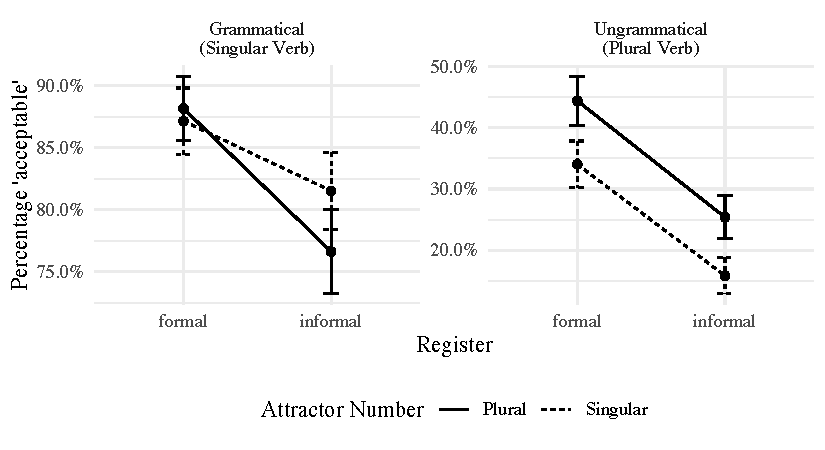
\includegraphics[width=\linewidth]{figure/exp4AvgResponse-1} 

}

\caption{The average percentage of acceptable responses according to the experimental conditions in Experiment 4}\label{fig:exp4AvgResponse}
\end{figure}

\end{knitrout}

We see that in both formal and informal registers, participants accepted sentences with plural attractor and verb (M = 0.44 and 0.25, SE = 0.02 and 0.02, for formal and informal registers, respectively) more often than singular attractor counterparts (M = 0.34 and 0.16, SE = 0.02 and 0.02, for formal and informal registers, respectively). This clearly shows that the agreement attraction effects were due to a possible honorific reading. 

As we expected, formal registers with words like \emph{sir} licensed the presence of a plural verbal agreement. However, due to the speaker variability, the acceptability of sentences with a plural verb in the formal register conditions (M = 0.44 and 0.34, SE = 0.02 and 0.02, for singular and plural attractor conditions, respectively) were not on par with the sentences with the singular verb in the formal register conditions (M = 0.88 and 0.87, SE = 0.01 and 0.01, for singular and plural attractor conditions, respectively). Interestingly, in informal registers, there is a slight difference between singular attractor (M = 0.82, SE = 0.02) and plural attractor conditions (M = 0.77, SE = 0.02) with plural verb. We also see that singular verbs in informal registers were accepted less often than those in the formal register conditions. 

Figure \ref{fig:exp4Bayes} shows the coefficient posterior summaries extracted from our Bayesian GLM fitted to the data from Experiment 4. On the right-hand side, we see the posterior probability of the effect of a coefficient being smaller than 0. The dot shows the mean estimate of the posteriors while the line indicates 95\% credible intervals.

\begin{knitrout}
\definecolor{shadecolor}{rgb}{0.969, 0.969, 0.969}\color{fgcolor}\begin{figure}[hbt!]

{\centering 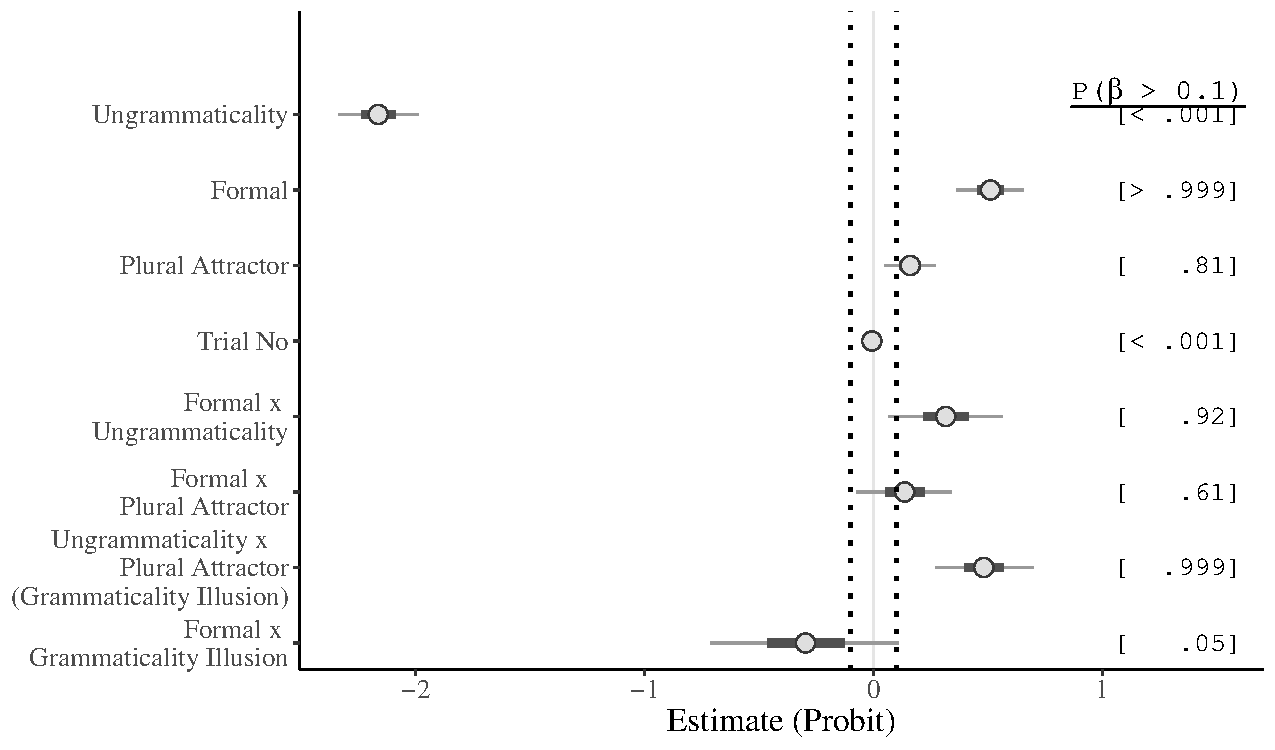
\includegraphics[width=\linewidth]{figure/exp4Bayes-1} 

}

\caption{Estimates and 95\% credible intervals for the probit regression coefficients for the model of responses in our Experiment 4}\label{fig:exp4Bayes}
\end{figure}

\end{knitrout}

The negative main effect of ungrammaticality ($\hat{\beta}=-2.16;$ $CI=[-2.38; -1.96];$ $P(\beta>0.1)< .001$) showed that participants were able to detect ungrammaticality. However, the estimate is smaller than our previous experiments because the formal register occasionally licensed the presence of plural agreement on the verb. The positive main effect of formal register ($\hat{\beta}=0.51;$ $CI=[0.33; 0.69];$ $P(\beta>0.1)> .999$) was expected given that it licenses the plural agreement. The clear positive effect of the interaction between the ungrammaticality and the plural attractor ($\hat{\beta}=0.48;$ $CI=[0.23; 0.75];$ $P(\beta>0.1)  .999$) showed that the percentage of acceptable responses in ungrammatical are amplified when the attractor is plural independent of the register. The weak negative interaction between the formal register, ungrammaticality, and the plural attractor ($\hat{\beta}=-0.30;$ $CI=[-0.79; 0.18];$ $P(\beta>0.1)   .05$) implied that the presence of an interjection that might induce formality decreased the amplification of the percentage of acceptable responses driven by the existence of plural attractor in ungrammatical sentences. 

\section{Discussion}

Experiment 4 investigated an alternative account for Turkish agreement attraction facts: a plural marker at the verb might induce an honorific reading and increase acceptability in ungrammatical sentences similar to the effects seen in attraction studies. We hypothesized that this honorific reading would not be possible with slang interjections like yo, dude, or lan in Turkish. We conducted a speeded acceptability judgment experiment with eight conditions to test this hypothesis. We manipulated the number of the verb (plural x singular), attractor (plural x singular), and the register (formal x informal).

Our results showed that formal interjections like \emph{sir} increased the overall acceptability in ungrammatical sentences, and the effect of plural attractor was present. More importantly, the same effect of plural attractor was also present in informal register with slang interjection endings. Our results were also certified in our Bayesian GLM: positive interaction between the verb plurality and the attractor plurality independent of the register. 

We can say that the initial findings of Turkish agreement attraction were not due to a formal reading licensing the plural verb. However, these results must be taken with caution since the experimental design was sub-optimal.



\chapter{ETHICS COMMITTEE APPROVAL} \label{ap:ethics}
\vspace*{-1cm}\hspace{-2cm}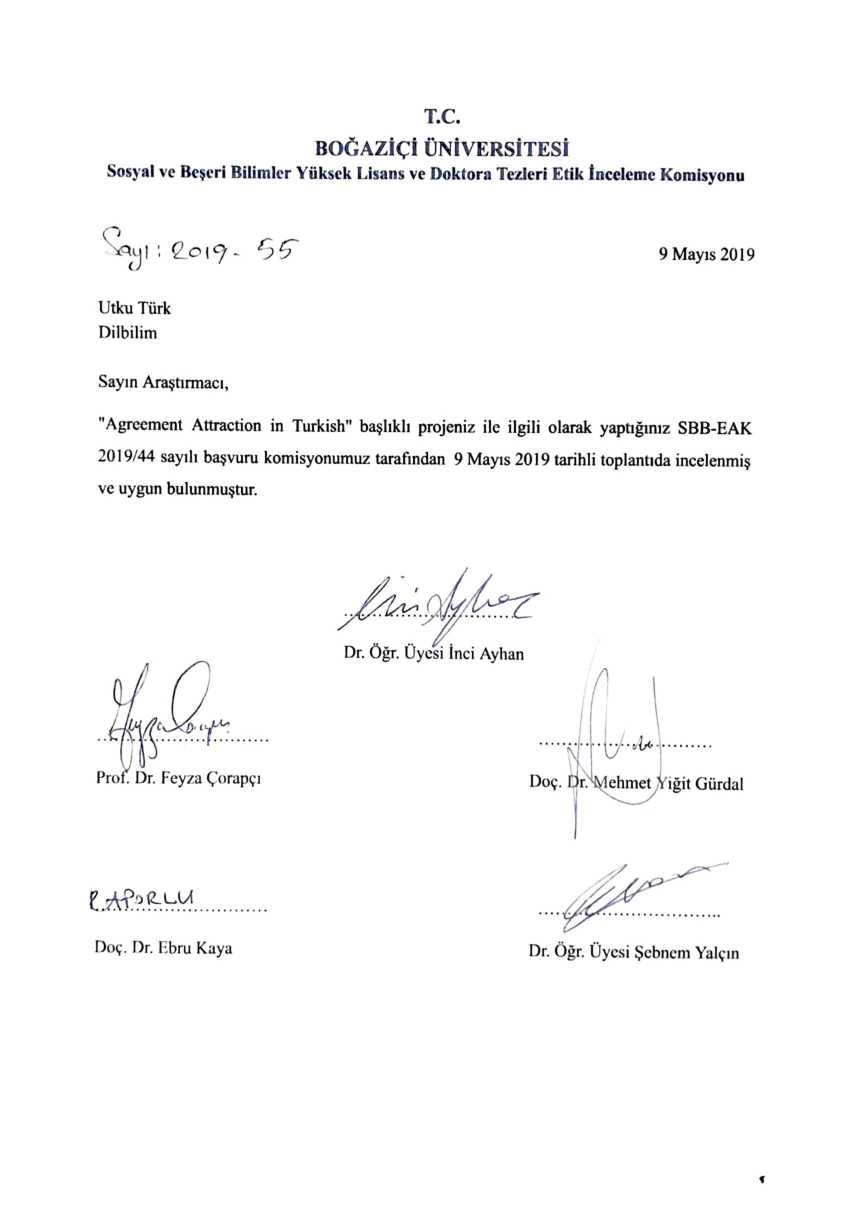
\includegraphics[width=1.10\textwidth]{figure/etik.pdf}


%% INCLUDE THE PDF HERE 

%\newpage
% \newcommand\blankpage{%
%     \null
%     \thispagestyle{empty}%
%     \addtocounter{page}{-1}%
%     \newpage}
    
% \afterpage{\blankpage}
%\doublespacing


\newpage



\chapter{EXPERIMENT 1 ITEMS} \label{ap:exp1items}

\section{Experimental items}

\ea Y\"{o}neticilerin/Y\"{o}neticinin a\c{s}\c{c}{\i}s{\i} mutfakta s\"{u}rekli z{\i}plad{\i}lar/z{\i}plad{\i}. \\* 
({\it The managers'/manager's cook jumped\textsubscript{PL/SG} constantly in the kitchen.})
\ex \"{O}\u{g}rencilerin/\"{O}\u{g}rencinin ablas{\i} s{\i}n{\i}fta birden bay{\i}ld{\i}lar/bay{\i}ld{\i}. \\* 
({\it The students'/student's older sister suddenly fainted\textsubscript{PL/SG} in class.})
\ex Marangozlar{\i}n/Marangozun abisi at\"{o}lyeden h{\i}zla uzakla\c{s}t{\i}lar/uzakla\c{s}t{\i}.\\* 
({\it The carpenters'/carpenter's older brother rushed\textsubscript{PL/SG} away from the workshop.})
\ex Mahallelilerin/Mahallelinin emlak\c{c}{\i}s{\i} aniden k\"{u}stah\c{c}a g\"{u}ld\"{u}ler/g\"{u}ld\"{u}.\\* 
({\it The residents'/resident's real estate agent suddenly laughed\textsubscript{PL/SG} arrogantly.})
\ex K{\i}zlar{\i}n/K{\i}z{\i}n halas{\i} sabaha kadar a\u{g}lad{\i}lar/a\u{g}lad{\i}.\\* 
({\it The girls'/girl's aunt cried\textsubscript{PL/SG} until morning.})
\ex Damatlar{\i}n/Damat{\i}n day{\i}s{\i} arada s{\i}rada s{\i}k{\i}ld{\i}lar/s{\i}k{\i}ld{\i}.\\* 
({\it Grooms'/Groom's uncle are bored\textsubscript{PL/SG} from time to time.})
\ex Doktorlar{\i}n/Doktorun \c{c}i\c{c}ek\c{c}isi g\"{u}nden g\"{u}ne zay{\i}flad{\i}lar/zay{\i}flad{\i}.\\* 
({\it The doctors'/doctor's florist got\textsubscript{PL/SG} thinner day by day.})
\ex Aristokratlar{\i}n/Aristokrat{\i}n hizmet\c{c}isi yorgun arg{\i}n yatt{\i}lar/yatt{\i}.\\*
({\it Aristocrats'/Aristocrat's maid slept\textsubscript{PL/SG} tiredly.})
\ex Konu\c{s}mac{\i}lar{\i}n/Konu\c{s}mac{\i}n{\i}n sunucusu ola\u{g}an\"{u}st\"{u} h{\i}zl{\i} ko\c{s}tular/ko\c{s}tu.\\*
({\it Speakers'/Speaker's presenter ran\textsubscript{PL/SG} extraordinarily fast.})
\ex Psikiyatristlerin/Psikiyatristin eczac{\i}s{\i} a\c{c} susuz dola\c{s}t{\i}lar/dola\c{s}t{\i}.\\*
({\it Psychiatrists'/Psychiatrist's pharmacist wandered\textsubscript{PL/SG} hungry and thirsty.})
\ex Politikac{\i}lar{\i}n/Politikac{\i}n{\i}n hocas{\i} adliyeden \c{c}abucak \c{c}{\i}kt{\i}lar/\c{c}{\i}kt{\i}.\\*
({\it The politicians'/politician's teacher quickly left\textsubscript{PL/SG} the courthouse.})
\ex Hakimlerin/Hakimin \c{c}ayc{\i}s{\i} nedensiz yere k{\i}zd{\i}lar/k{\i}zd{\i}.\\*
({\it Judges'/Judge's tea-maker got\textsubscript{PL/SG} angry for no reason.})
\ex Oyuncular{\i}n/Oyuncunun hem\c{s}iresi etrafta ama\c{c}s{\i}zca gezdiler/gezdi.\\*
({\it Actors'/Actor's nurse wandered\textsubscript{PL/SG} around aimlessly.})
\ex \"{O}\u{g}retmenlerin/\"{O}\u{g}retmenin m\"{u}diresi biraz \"{o}nce arad{\i}lar/arad{\i}.\\*
({\it Teachers'/Teacher's headmistress just called\textsubscript{PL/SG}.})
\ex Milyonerlerin/Milyonerin terzisi tamamen gereksizce ba\u{g}{\i}rd{\i}lar/ba\u{g}{\i}rd{\i}.\\*
({\it The millionaires'/millionaire's tailor yelled\textsubscript{PL/SG} completely unnecessarily.})
\ex Bebeklerin/Bebek\u{g}in bak{\i}c{\i}s{\i} \c{c}ok kibar davrand{\i}lar/davrand{\i}.\\*
({\it Babies'/The baby caretaker was/were very kind.})
\ex \c{C}ocuklar{\i}n/\c{C}ocu\u{g}un dad{\i}s{\i} y\"{u}ksek sesle konu\c{s}tular/konu\c{s}tu.\\*
({\it The children's/child's nanny spoke\textsubscript{PL/SG} loudly.})
\ex Futbolcular{\i}n/Futbolcunun s\"{u}r\"{u}c\"{u}s\"{u} \c{c}ok yava\c{s} \c{c}al{\i}\c{s}t{\i}lar/\c{c}al{\i}\c{s}t{\i}.\\*
({\it The players'/player's driver ran\textsubscript{PL/SG} very slowly.})
\ex Modac{\i}lar{\i}n/Modac{\i}n{\i}n taksicisi saatlerce durmaks{\i}z{\i}n i\c{c}tiler/i\c{c}ti.\\*
({\it The fashionistas'/fashionista's taxi driver drank\textsubscript{PL/SG} non-stop for hours.})
\ex Sanat\c{c}{\i}lar{\i}n/Sanat\c{c}{\i}n{\i}n \c{c}alg{\i}c{\i}s{\i} feci bir \c{s}ekilde \"{o}ld\"{u}ler/\"{o}ld\"{u}.\\*
({\it The artists'/artist's instrumentalist died\textsubscript{PL/SG} tragically.})
\ex Dedektiflerin/Dedektifin di\c{s}\c{c}isi ilk kez \c{c}{\i}lg{\i}nca e\u{g}lendiler/e\u{g}lendi.\\*
({\it The detectives'/detective's dentist had\textsubscript{PL/SG} a blast for the first time.})
\ex Esnaflar{\i}n/Esnaf{\i}n m\"{u}\c{s}terisi \c{s}ikayettten hemen sonra sustular/sustu.\\*
({\it The shopkeepers'/shopkeeper's customer fell\textsubscript{PL/SG} silent immediately after complaining.})
\ex \c{S}ark{\i}c{\i}lar{\i}n/\c{S}ark{\i}c{\i}n{\i}n korumas{\i} her zamanki gibi geciktiler/gecikti.\\*
({\it The singers'/singer's bodyguard was/were delayed as usual.})
\ex G\"{o}stericilerin/G\"{o}stericinin izleyicisi ak\c{s}ama kadar sessizce oturdular/oturdu.\\*
({\it The demonstrators'/demonstrator's audience sat\textsubscript{PL/SG} in silence until the evening.})
\ex Cerrahlar{\i}n/Cerrah{\i}n hastas{\i} ak\c{s}amki g\"{o}steriden \"{o}nce ka\c{c}t{\i}lar/ka\c{c}t{\i}.\\*
({\it The surgeons'/surgeon's patients fled\textsubscript{PL/SG} before the evening's performance.})
\ex Dalg{\i}\c{c}lar{\i}n/Dalg{\i}\c{c}{\i}n annesi bile bile ge\c{c} kald{\i}lar/kald{\i}.\\*
({\it The divers'/diver's mother was/were late on purpose.})
\ex Fabrikat\"{o}rlerin/Fabrikat\"{o}r\"{u}n i\c{s}\c{c}isi beklenmedik bir anda hastaland{\i}lar/hastaland{\i}.\\*
({\it Fabricators'/Fabricator's worker got\textsubscript{PL/SG} sick unexpectedly.})
\ex Komedyenlerin/Komedyenin yard{\i}mc{\i}s{\i} poyrazdan dolay{\i} \"{u}\c{s}\"{u}d\"{u}ler/\"{u}\c{s}\"{u}d\"{u}.\\*
({\it The comedians'/comedian's assistant was/were cold because of the bad wind.})
\ex \c{S}of\"{o}rlerin/\c{S}of\"{o}r\"{u}n yolcusu yemekten sonra yine ac{\i}kt{\i}lar/ac{\i}kt{\i}.\\*
({\it Drivers'/Driver's passenger got\textsubscript{PL/SG} hungry again after dinner.})
\ex M\"{u}hendislerin/M\"{u}hendisin kap{\i}c{\i}s{\i} erken \"{o}demeden dolay{\i} sevindiler/sevindi.\\*
({\it Engineers'/Engineer's doorman delighted\textsubscript{PL/SG} with early payment.})
\ex Pazarc{\i}lar{\i}n/Pazarc{\i}n{\i}n nakliyecisi mesaiden hemen sonra uzand{\i}lar/uzand{\i}.\\*
({\it The marketers'/marketer's shipper lay\textsubscript{PL/SG} down right after work.})
\ex Oyuncular{\i}n/Oyuncunun e\u{g}itimcisi ilk denemede epey zorland{\i}lar/zorland{\i}.\\*
({\it Players'/Player's trainer struggled\textsubscript{PL/SG} on the first try.})
\ex Mankenlerin/Mankenin modac{\i}s{\i} ge\c{c} bir vakitte kalkt{\i}lar/kalkt{\i}.\\*
({\it The mannequins'/The mannequin's fashionista got\textsubscript{PL/SG} up late.})
\ex Konuklar{\i}n/Konu\u{g}un teyzesi m\"{u}thi\c{s} bir a\u{g}r{\i}yla uyand{\i}lar/uyand{\i}.\\*
({\it Guests'/Guest's aunt woke\textsubscript{PL/SG} up with excruciating pain.})
\ex O\u{g}lanlar{\i}n/O\u{g}lan{\i}n amcas{\i} bo\c{s} bir caddede y\"{u}r\"{u}d\"{u}ler/y\"{u}r\"{u}d\"{u}.\\*
({\it The boys'/boy's uncle walked\textsubscript{PL/SG} down an empty street.})
\ex Avukatlar{\i}n/Avukat{\i}n kom\c{s}usu toplant{\i}dan sonra birden sarard{\i}lar/sarard{\i}.\\*
({\it The lawyers'/lawyer's neighbor suddenly turned\textsubscript{PL/SG} yellow after the meeting.})
\ex \"{U}nl\"{u}lerin/\"{U}nl\"{u}n\"{u}n falc{\i}s{\i} yabanc{\i} bir \"{u}lkede kayboldular/kayboldu.\\*
({\it Celebrities'/Celebrity's fortune teller got\textsubscript{PL/SG} lost in a foreign country.})
\ex \c{C}ift\c{c}ilerin/\c{C}ift\c{c}inin bek\c{c}isi normalden \c{c}ok yava\c{s} gezindiler/gezindi.\\*
({\it The Farmers'/Farmer's guard roamed\textsubscript{PL/SG} a lot slower than usual.})
\ex Kad{\i}nlar{\i}n/Kad{\i}n{\i}n ninesi ge\c{c}en seneye g\"{o}re din\c{c}le\c{s}tiler/din\c{c}le\c{s}ti.\\*
({\it Women's/Woman's grandmother became\textsubscript{PL/SG} more vigorous compared to last year.})
\z

\section{Filler items}
\ea {Grammatical Fillers}
\ea Adam{\i}n annesi fenala\c{s}{\i}nca inek kurban ettiler.\\*
({\it When the man's mother fell ill, they sacrificed a cow.})
\ex Sosyologun \"{o}\u{g}rencisi konu\c{s}unca tutars{\i}zl{\i}k a\c{c}{\i}\u{g}a \c{c}{\i}kard{\i}lar.\\*
({\it When the sociologist's student spoke, they revealed inconsistency.})
\ex Doktorun hem\c{s}iresi gelene kadar hasta taburcu ettiler.\\*
({\it The patient was discharged until the doctor's nurse arrived.})
\ex Kemanc{\i}n{\i}n sevgilisi \"{o}l\"{u}nce mezar ziyaret ettiler.\\*
({\it When the violinist's lover died, they visited a grave.})
\ex Hocan{\i}n kap{\i}c{\i}s{\i} bay{\i}l{\i}nca doktor rahats{\i}z ettiler.\\*
({\it When the teacher's doorman fainted, they bothered a doctor.})
\ex Medyumun kocas{\i} sa\c{c}malay{\i}nca falc{\i} zengin ettiler.\\*
({\it When the psychic's husband made nonsense, they made the fortune-teller rich.})
\ex Ba\c{s}kan{\i}n di\c{s}\c{c}isi t{\i}rs{\i}nca stajyer kabul ettiler.\\*
({\it When the president's dentist got scared, they accepted a trainee.})
\ex Ele\c{s}tirmenin kar{\i}s{\i} k{\i}v{\i}rt{\i}nca sap{\i}k tahrik ettiler.\\*
({\it Perverted aroused when the critic's wife squirmed.})
\ex Patronun kahyas{\i} d\"{u}\c{s}\"{u}nce d\"{u}\c{s}man mutlu ettiler.\\*
({\it When the boss's butler fell, they made an enemy happy.})
\ex M\"{u}d\"{u}r\"{u}n a\c{s}\c{c}{\i}s{\i} haz{\i}rlan{\i}nca yemek haz{\i}r ettiler.\\*
({\it When the manager's cook was ready, they prepared a meal.})
\ex \c{C}ocu\u{g}un abisi \"{u}z\"{u}l\"{u}nce oyuncak icat ettiler.\\*
({\it When the boy's brother was upset, they invented a toy.})
\ex Psikologun hastas{\i} gecikince vakit hi\c{c} ettiler.\\*
({\it When the psychologist's patient was late, they killed some time.})
\ex Ressam{\i}n tedarik\c{c}isi kaybolunca tuval ithal ettiler.\\*
({\it When the painter's supplier disappeared, they imported canvas.})
\ex Di\c{s}\c{c}inin temizlik\c{c}isi yorulunca hademe ikna ettiler.\\*
({\it When the dentist's housekeeper got tired, they convinced the janitor.})
\ex Kimyagerin kuryesi hap\c{s}urunca deney ak{\i}l ettiler.\\*
({\it When the chemist's courier sneezed, they came up with the experiment.})
\ex Mankenin motorcusu s{\i}z{\i}nca \c{c}{\i}rak me\c{s}gul ettiler.\\*
({\it They kept the apprentice busy when the model's biker fell asleep.})
\ex Dekan{\i}n davetlisi ge\c{c}ince seyirci aya\u{g}a kald{\i}rd{\i}lar.\\*
({\it When the dean's guest passed, they made the audience stood up.})
\ex Mafyan{\i}n yat{\i}r{\i}mc{\i}s{\i} bat{\i}nca kuyumcu tehdit ettiler.\\*
({\it When the investor of the mafia went bankrupt, they threatened the jeweler.})
\ex A\c{s}\c{c}{\i}n{\i}n manav{\i} kapan{\i}nca et tedarik ettiler.\\*
({\it When the cook's grocer closed, they supplied meat.})
\ex \"{O}\u{g}rencinin hocas{\i} anlat{\i}nca makine icat ettiler.\\*
({\it When the student's teacher told them, they invented a machine.})
\z
\ex {Ungrammatical Fillers}
\ea * Bakan{\i}n yard{\i}mc{\i}s{\i} bulununca koltuk geri getirdi.\\*
({\it * When the deputy minister was found, the chair brought back.})
\ex * \"{O}\u{g}rencinin hocas{\i} ayr{\i}l{\i}nca proje birden unuttu.\\*
({\it * The project was suddenly forgot when the student's teacher left.})
\ex * Pizzac{\i}n{\i}n kuryesi t\"{o}kezleyince soslar yere sa\c{c}t{\i}.\\*
({\it *  When the pizzeria's courier stumbled, sauces spilled onto the floor.})
\ex * Kral{\i}n soytar{\i}s{\i} as{\i}l{\i}nca \c{s}apka yerinde buldu.\\*
({\it * When the king's jester was hanged, the hat found in its place.})
\ex * Dekan{\i}n davetlisi hap\c{s}urunca \c{c}aylar aniden d\"{u}\c{s}\"{u}rd\"{u}.\\*
({\it * The dean's guest sneezed, and the tea suddenly dropped.})
\ex * Dedektifin g\"{o}zl\"{u}k\c{c}\"{u}s\"{u} evlenince hediyeler a\u{g}lanarak verdi.\\*
({\it * When the detective's optician got married, he gave presents crying.})
\ex * Politikac{\i}n{\i}n s\"{o}zc\"{u}s\"{u} yakalan{\i}nca a\c{c}{\i}klama haliyle kesti.\\*
({\it * When the politician's spokesperson was caught, the statement naturally cut off.})
\ex * Kad{\i}n{\i}n temizlik\c{c}isi bay{\i}l{\i}nca deterjan tekrar sa\c{c}t{\i}.\\*
({\it * When the woman's housekeeper fainted, the detergent spilled out again.})
\ex * Mankenin ni\c{s}anl{\i}s{\i} vurulunca haber h{\i}zl{\i}ca yayd{\i}.\\*
({\it * News spread quickly when the model's fiancee was shot.})
\ex * \c{C}oban{\i}n s\"{o}zl\"{u}s\"{u} tutuklan{\i}nca kamera sessizce s\"{o}kt\"{u}.\\*
({\it * The camera discharge when the shepherd's spokesman was arrested.})
\ex * Dans\"{o}z\"{u}n kocas{\i} var{\i}nca kap{\i} sakince a\c{c}t{\i}.\\*
({\it * The door opened calmly when the dancer's husband arrived.})
\ex * \c{C}evirmenin kaynanas{\i} aramay{\i}nca metin keyfince bitirdi.\\*
({\it * When the translator's mother-in-law did not call, the text finished arbitrarily.})
\ex * Fabrikat\"{o}r\"{u}n muhasebecisi kovulunca hesap tamamen kar{\i}\c{s}t{\i}rd{\i}.\\*
({\it * The account completely messed up when the fabricator's accountant was fired.})
\ex * \"{U}nl\"{u}n\"{u}n k\"{u}rk\c{c}\"{u}s\"{u} d\"{o}n\"{u}nce kuma\c{s} erkenden dikti.\\*
({\it * When the famous furrier returned, the fabric sewed early.})
\ex * Rekt\"{o}r\"{u}n yard{\i}mc{\i}s{\i} atan{\i}nca k\"{u}t\"{u}phane gece kapatt{\i}.\\*
({\it * The library closed at night when the vice-chancellor was appointed.})
\ex * \c{S}ark{\i}c{\i}n{\i}n taksicisi gecikince trafik aniden kilitledi.\\*
({\it * When the singer's taxi driver was late, traffic suddenly locked.})
\ex * \c{C}ocu\u{g}un dad{\i}s{\i} aramay{\i}nca bula\c{s}{\i}k saatlerce y{\i}kad{\i}.\\*
({\it * The dishes cleanerd for hours when the boy's nanny didn't call.})
\ex * \c{C}ift\c{c}inin tesisat\c{c}{\i}s{\i} gelince borular g\"{u}\c{c}l\"{u}kle s\"{o}kt\"{u}.\\*
({\it * When the farmer's plumber came, the pipes had to remove with difficulty.})
\ex * \c{C}iftin mobilyac{\i}s{\i} k{\i}z{\i}nca koltuk sinirle par\c{c}alad{\i}.\\*
({\it * When the couple's furniture maker got angry, the sofa smashed in anger.})
\ex * Adam{\i}n falc{\i}s{\i} yan{\i}l{\i}nca fincan \"{o}fkeyle k{\i}rd{\i}.\\*
({\it * When the man's fortune teller was wrong, the cup broke in anger.})
\z
\z


\newpage


\chapter{EXPERIMENT 2A ITEMS} \label{ap:exp2aitems}
\section{Experimental items}

\ea D\"{o}vd\"{u}kleri/D\"{o}vd\"{u}\u{g}\"{u} \c{c}ocuk okula yorgun arg{\i}n geldiler/geldi.\\*
({\it The boy they/he beaten came\textsubscript{PL/SG} to school exhausted.})
\ex Tuttuklar{\i}/Tuttu\u{g}u a\c{s}\c{c}{\i} mutfakta s\"{u}rekli z{\i}plad{\i}lar/z{\i}plad{\i}.\\*
({\it The cook they/he hired bounced\textsubscript{PL/SG} around in the kitchen.})
\ex Tan{\i}d{\i}klar{\i}/Tan{\i}d{\i}\u{g}{\i} m\"{u}d\"{u}r s{\i}n{\i}fta birden bay{\i}ld{\i}lar/bay{\i}ld{\i}.\\*
({\it The principal they/he knew fainted\textsubscript{PL/SG} in class.})
\ex G\"{o}rd\"{u}kleri/G\"{o}rd\"{u}\u{g}\"{u} marangoz at\"{o}lyeden h{\i}zla uzakla\c{s}t{\i}lar/uzakla\c{s}t{\i}.\\*
({\it The carpenter they/he saw hurried\textsubscript{PL/SG} away from the workshop.})
\ex Azarlad{\i}klar{\i}/Azarlad{\i}\u{g}{\i} emlak\c{c}{\i} aniden k\"{u}stah\c{c}a g\"{u}ld\"{u}ler/g\"{u}ld\"{u}.\\*
({\it The realtor they/he scolded suddenly laughed\textsubscript{PL/SG} arrogantly.})
\ex Reddetikleri/Reddeti\u{g}i akademisyen sabaha kadar a\u{g}lad{\i}lar/a\u{g}lad{\i}.\\*
({\it The academic, whom they/he rejected, wept\textsubscript{PL/SG} until the morning.})
\ex Beklettikleri/Beklettik\u{g}i ara\c{s}t{\i}rmac{\i} g\"{u}n boyunca s{\i}k{\i}ld{\i}lar/s{\i}k{\i}ld{\i}.\\*
({\it The investigator they/he were holding was/were bored during the day.})
\ex Bakt{\i}klar{\i}/Bakt{\i}\u{g}{\i} hasta g\"{u}nden g\"{u}ne zay{\i}flad{\i}lar/zay{\i}flad{\i}.\\*
({\it The patient they/he cared for got\textsubscript{PL/SG} weaker day by day.})
\ex Yorduklar{\i}/Yordu\u{g}u oyuncu onikiden \"{o}nce uyudular/uyudu.\\*
({\it The player they/he wore down fell\textsubscript{PL/SG} asleep before twelve.})
\ex \c{C}al{\i}\c{s}t{\i}rd{\i}klar{\i}/\c{C}al{\i}\c{s}t{\i}rd{\i}\u{g}{\i} hizmet\c{c}i yorgun arg{\i}n yatt{\i}lar/yatt{\i}.\\*
({\it The maid they/he hired went\textsubscript{PL/SG} to bed tiredly.})
\ex Kovduklar{\i}/Kovdu\u{g}u sunucu ola\u{g}an\"{u}st\"{u} bir h{\i}zla konu\c{s}tular/konu\c{s}tu.\\*
({\it The server they/he fired spoke\textsubscript{PL/SG} with extraordinary speed.})
\ex Kaybettikleri/Kaybetti\u{g}i turist a\c{c} susuz dola\c{s}t{\i}lar/dola\c{s}t{\i}.\\*
({\it The tourist they/he lost wandered\textsubscript{PL/SG} around hungry and thirsty.})
\ex Cezaland{\i}rd{\i}klar{\i}/Cezaland{\i}rd{\i}\u{g}{\i} hoca hapisten \c{c}abucak \c{c}{\i}kt{\i}lar/\c{c}{\i}kt{\i}.\\*
({\it The teacher they/he punished\textsubscript{PL/SG} quickly got out of jail.})
\ex Uyand{\i}rd{\i}klar{\i}/Uyand{\i}rd{\i}\u{g}{\i} \c{c}ayc{\i} nedensiz yere k{\i}zd{\i}lar/k{\i}zd{\i}.\\*
({\it The tea shop they/he woke\textsubscript{PL/SG} up got angry for no reason.})
\ex Susturduklar{\i}/Susturdu\u{g}u hem\c{s}ire etrafta ama\c{c}s{\i}zca gezdiler/gezdi.\\*
({\it The nurse they/he had silenced wandered\textsubscript{PL/SG} around aimlessly.})
\ex Sorduklar{\i}/Sordu\u{g}u m\"{u}dire biraz \"{o}nce arad{\i}lar/arad{\i}.\\*
({\it The manager they/he asked just called\textsubscript{PL/SG}.})
\ex G\"{o}nderdikleri/G\"{o}nderdi\u{g}i terzi tamamen gereksizce ba\u{g}{\i}rd{\i}lar/ba\u{g}{\i}rd{\i}.\\*
({\it The tailor they/he sent yelled\textsubscript{PL/SG} completely unnecessarily.})
\ex Bulduklar{\i}/Bulduk\u{g}u bak{\i}c{\i} \c{c}ok kibar davrand{\i}lar/davrand{\i}.\\*
({\it The caretaker they/he found was/were very kind.})
\ex Be\u{g}endikleri/Be\u{g}endi\u{g}i dad{\i} sahil boyunca s\"{u}z\"{u}ld\"{u}ler/s\"{u}z\"{u}ld\"{u}.\\*
({\it The nanny they/he liked glided\textsubscript{PL/SG} along the beach.})
\ex Ara\c{s}t{\i}rd{\i}klar{\i}/Ara\c{s}t{\i}rd{\i}\u{g}{\i} tamirci \c{c}ok yava\c{s} \c{c}al{\i}\c{s}t{\i}lar/\c{c}al{\i}\c{s}t{\i}.\\*
({\it The mechanic they/he searched worked\textsubscript{PL/SG} very slowly.})
\ex Efkarland{\i}rd{\i}klar{\i}/Efkarland{\i}rd{\i}\u{g}{\i} taksici saatlerce durmaks{\i}z{\i}n i\c{c}tiler/i\c{c}ti.\\*
({\it The taxi driver they/he made nostalgic drank\textsubscript{PL/SG} nonstop for hours.})
\ex Kovalad{\i}klar{\i}/Kovalad{\i}\u{g}{\i} \c{c}alg{\i}c{\i} feci bir \c{s}ekilde \"{o}ld\"{u}ler/\"{o}ld\"{u}.\\*
({\it The instrumentalist they/he chased died\textsubscript{PL/SG} horribly.})
\ex Gittikleri/Gitti\u{g}i di\c{s}\c{c}i ilk kez \c{c}{\i}lg{\i}nca e\u{g}lendiler/e\u{g}lendi.\\*
({\it The dentist they/he went to had\textsubscript{PL/SG} fun for the first time.})
\ex A\u{g}latt{\i}klar{\i}/A\u{g}latt{\i}\u{g}{\i} m\"{u}\c{s}teri \c{s}ikayetinden hemen sonra sustular/sustu.\\*
({\it The customer they/he made cry shut\textsubscript{PL/SG} up immediately after his complaint.})
\ex \c{C}{\i}ld{\i}rtt{\i}klar{\i}/\c{C}{\i}ld{\i}rtt{\i}\u{g}{\i} koruma her zamanki gibi geciktiler/gecikti.\\*
({\it The bodyguard they/he drove crazy delayed\textsubscript{PL/SG} as usual.})
\ex Getirdikleri/Getirdi\u{g}i izleyici ak\c{s}ama kadar sessizce oturdular/oturdu.\\*
({\it The audience they/he brought sat\textsubscript{PL/SG} in silence until the evening.})
\ex Delirttikleri/Delirtti\u{g}i hasta ak\c{s}amki muayeneden \"{o}nce ka\c{c}t{\i}lar/ka\c{c}t{\i}.\\*
({\it The patient they/he had driven mad fled\textsubscript{PL/SG} before the evening's examination.})
\ex Anla\c{s}t{\i}klar{\i}/Anla\c{s}t{\i}\u{g}{\i} terapist bile bile ge\c{c} kald{\i}lar/kald{\i}.\\*
({\it The therapist they/he hired was/were late on purpose.})
\ex G\"{u}vendikleri/G\"{u}vendi\u{f}i i\c{s}\c{c}i beklenmedik bir anda hastaland{\i}lar/hastaland{\i}.\\*
({\it The employee they/he trusted fell\textsubscript{PL/SG} ill unexpectedly.})
\ex E\u{g}ittikleri/E\u{g}itti\u{g}i hostes sert r\"{u}zgarlardan dolay{\i} \"{u}\c{s}\"{u}d\"{u}ler/\"{u}\c{s}\"{u}d\"{u}.\\*
({\it The stewardess they/he trained got\textsubscript{PL/SG} cold from the strong winds.})
\ex Doyurduklar{\i}/Doyurdu\u{g}u yolcu yemekten sonra yine ac{\i}kt{\i}lar/ac{\i}kt{\i}.\\*
({\it The passengers they/he fed got\textsubscript{PL/SG} hungry again after the meal.})
\ex \c{C}a\u{g}{\i}rd{\i}klar{\i}/\c{C}a\u{g}{\i}rd{\i}\u{g}{\i} kap{\i}c{\i} erken \"{o}demeden dolay{\i} sevindiler/sevindi.\\*
({\it The concierge they/he called was/were happy with the early payment.})
\ex Yorduklar{\i}/Yordu\u{g}u nakliyeci mesaiden hemen sonra uzand{\i}lar/uzand{\i}.\\*
({\it The shipper they/he had tired of lay\textsubscript{PL/SG} down right after work.})
\ex Yeti\c{s}tirdikleri/Yeti\c{s}tirdi\u{g}i e\u{g}itimci ilk denemede epey zorland{\i}lar/zorland{\i}.\\*
({\it The trainer they/he trained had\textsubscript{PL/SG} a hard time on the first try.})
\ex Kiralad{\i}klar{\i}/Kiralad{\i}\u{g}{\i} animat\"{o}r ge\c{c} bir vakitte kalkt{\i}lar/kalkt{\i}.\\*
({\it The animator they/he hired got\textsubscript{PL/SG} up late.})
\ex Yaralad{\i}klar{\i}/Yaralad{\i}\u{g}{\i} polis m\"{u}thi\c{s} bir a\u{g}r{\i}yla uyand{\i}lar/uyand{\i}.\\*
({\it The cop they/he had injured woke\textsubscript{PL/SG} up in terrible pain.})
\ex Ka\c{c}{\i}rd{\i}klar{\i}/Ka\c{c}{\i}rd{\i}\u{g}{\i} h{\i}rs{\i}z bo\c{s} bir caddede y\"{u}r\"{u}d\"{u}ler/y\"{u}r\"{u}d\"{u}.\\*
({\it The thief they/he kidnapped walked\textsubscript{PL/SG} down an empty street.})
\ex Zehirledikleri/Zehirledi\u{g}i kral toplant{\i}dan sonra birden sarard{\i}lar/sarard{\i}.\\*
({\it The king they/he poisoned turned\textsubscript{PL/SG} pale after the meeting.})
\ex Gezdirdikleri/Gezdirdi\u{g}i falc{\i} yabanc{\i} bir \"{u}lkede kayboldular/kayboldu.\\*
({\it The fortune teller they/he showed around got\textsubscript{PL/SG} lost in a foreign country.})
\ex \c{S}\"{u}phelendirdikleri/\c{S}\"{u}phelendirdi\u{g}i bek\c{c}i normalden \c{c}ok yava\c{s} gezindiler/gezindi.\\*
({\it The guard they/he suspected roamed\textsubscript{PL/SG} much slower than normal.})
\z

\section{Filler items}
\ea {Grammatical Fillers}
\ea Okuttuklar{\i} \"{o}\u{g}renci ba\c{s}ar{\i}l{\i} olunca mutlu oldular. \\*
({\it They were happy when the student they sponsored was successful.})
\ex Biriktirdikleri para d\"{u}n kaybolunca \c{c}{\i}lg{\i}na d\"{o}nd\"{u}ler. \\*
({\it They went crazy when their savings disappeared yesterday.})
\ex D\"{u}\c{s}\"{u}nd\"{u}kleri teknisyen h{\i}zl{\i} \c{c}al{\i}\c{s}t{\i}\u{g}{\i}ndan tekrar \c{c}a\u{g}{\i}rd{\i}lar. \\*
({\it They called again because the technician they thought about was working fast.})
\ex Haz{\i}rlad{\i}klar{\i} yemek yere d\"{o}k\"{u}l\"{u}nce yenisini yapt{\i}lar. \\*
({\it When the food they prepared spilled on the floor, they made a new one.})
\ex Ba\c{s}lad{\i}klar{\i} film k\"{o}t\"{u} \c{c}{\i}k{\i}nca dizi izlediler. \\*
({\it When the movie they started watching was bad, they watched a TV series.})
\ex Diktikleri a\u{g}a\c{c} meyve verince epey \c{s}a\c{s}{\i}rd{\i}lar. \\*
({\it They were quite surprised when the tree they planted bore fruit.})
\ex Sevdikleri \"{o}\u{g}retmen emekli olunca saatlerce a\u{g}lam{\i}\c{s}lar. \\*
({\it They cried for hours when their favorite teacher retired.})
\ex Kulland{\i}klar{\i} ila\c{c} rahats{\i}z edince doktorla konu\c{s}mu\c{s}lar. \\*
({\it They talked to the doctor when the medication they used bothered them.})
\ex S\"{o}yledikleri yemek so\u{g}uk gelince geri g\"{o}nderdiler. \\*
({\it When the food they ordered was cold, they sent it back.})
\ex Ay{\i}plad{\i}klar{\i} kad{\i}n onlar{\i} duyunca biraz gerildiler. \\*
({\it When the woman they blamed heard them, they got a little nervous.})
\ex Bahsettikleri \"{u}nl\"{u} kafeye gelince \c{s}ok olmu\c{s}lar. \\*
({\it They were shocked when the famous person they were talking about came to the cafe.})
\ex Bindikleri araba sorun \c{c}{\i}kar{\i}nca hemen indiler. \\*
({\it When the car they were in caused trouble, they got off immediately.})
\ex Okuduklar{\i} \c{s}iir seyirciler taraf{\i}ndan be\u{g}enilmeyince \"{u}z\"{u}ld\"{u}ler. \\*
({\it They were upset when the poem they read was not liked by the audience.})
\ex Dinledikleri \c{s}ark{\i}c{\i} yanlar{\i}na gelince a\c{s}{\i}r{\i} heyecanland{\i}lar. \\*
({\it They got very excited when the singer they were listening to came to them.})
\ex Ka\c{c}t{\i}klar{\i} katil durunca rahat bir nefes ald{\i}lar. \\*
({\it They breathed a sigh of relief when the killer they were running from stopped.})
\ex Kar\c{s}{\i}la\c{s}t{\i}klar{\i} \c{c}ocuk kayboldu\u{g}u i\c{c}in olduk\c{c}a endi\c{s}elenmi\c{s}ler. \\*
({\it They were very worried that the boy they met had disappeared.})
\ex Ald{\i}klar{\i} elma kurtland{\i}\u{g}{\i} i\c{c}in atmak zorunda kald{\i}lar. \\*
({\it The apple they bought got wormy so they had to throw it away.})
\ex K{\i}rd{\i}klar{\i} tabak kolayca yap{\i}\c{s}t{\i}r{\i}l{\i}nca yenisini almad{\i}lar. \\*
({\it The plate they broke was easily glued, so they didn't get a new one.})
\ex Yapt{\i}klar{\i} heykel ya\u{g}murda {\i}slan{\i}nca kurulamaya giri\c{s}tiler. \\*
({\it When the statue they made got wet in the rain, they started to dry it.})
\ex G{\i}d{\i}klad{\i}klar{\i} bebek \"{u}stlerine kusunca banyoya ko\c{s}tular. \\*
({\it When the baby they tickled vomited on them, they ran to the bathroom.})
\z
\ex {Ungrammatical Fillers}
\ea * K{\i}zd{\i}\u{g}{\i} bakan bulununca koltuk geri getirdi. \\*
({\it * When the minister whom he was angry at was found, the chair brought back.})
\ex * Arad{\i}\u{g}{\i} asistan ayr{\i}l{\i}nca proje birden unuttu. \\*
({\it * When the assistant he was looking for left, the project suddenly forgot.})
\ex * Bekledi\u{g}i kurye t\"{o}kezleyince soslar yere sa\c{c}t{\i}. \\*
({\it * When the courier he was waiting for stumbled, sauces spilled on the floor.})
\ex * G\"{u}ld\"{u}\u{g}\"{u} soytar{\i} as{\i}l{\i}nca \c{s}apka yerinde buldu. \\*
({\it * When the jester he laughed at was hanged, the hat found in its place.})
\ex * Yaz{\i}\c{s}t{\i}\u{g}{\i} dekan hap\c{s}urunca \c{c}aylar aniden d\"{u}\c{s}\"{u}rd\"{u}. \\*
({\it * The dean he corresponded with sneezed, the tea suddenly dropped.})
\ex * Bildi\u{g}i g\"{o}zl\"{u}k\c{c}\"{u} evlenince hediyeler a\u{g}lanarak verdi. \\*
({\it * When the optician he knew got married, gifts gave while crying.})
\ex * Savundu\u{g}u politikac{\i} yakalan{\i}nca a\c{c}{\i}klama haliyle kesti. \\*
({\it * When the politician he was defending was caught, the statement cut.})
\ex * A\u{g}{\i}rlad{\i}\u{g}{\i} temizlik\c{c}i bay{\i}l{\i}nca deterjan tekrar sa\c{c}t{\i}. \\*
({\it * When the housekeeper he was hosting fainted, the detergent spilled again.})
\ex * D\"{u}\c{s}ledi\u{g}i manken ni\c{s}anlan{\i}nca haber h{\i}zl{\i}ca yayd{\i}. \\*
({\it * The news spread quickly when the mannequin of her dreams got engaged.})
\ex * S\"{o}zle\c{s}ti\u{g}i fabrikat\"{o}r vurulunca kamera sessizce s\"{o}kt\"{u}. \\*
({\it * The camera silently dismantled when the fabricator he engaged with was shot.})
\ex * {\.I}stedi\u{g}i dans\"{o}z var{\i}nca kap{\i} sakince a\c{c}t{\i}. \\*
({\it * The door calmly opened when the belly dancer he wanted arrived.})
\ex * Haberle\c{s}ti\u{g}i \c{c}evirmen aramay{\i}nca metin keyfince bitirdi. \\*
({\it * When the translator with whom he communicated did not call, the text ended arbitrarily.})
\ex * Ba\u{g}{\i}rd{\i}\u{g}{\i} muhasebeci kovulunca hesap tamamen kar{\i}\c{s}t{\i}rd{\i}. \\*
({\it * The account completely messed up when the accountant he shouted was fired.})
\ex * Bulu\c{s}tu\u{g}u k\"{u}rk\c{c}\"{u} d\"{o}n\"{u}nce kuma\c{s} erkenden dikti. \\*
({\it * When the furrier he met returned, the fabric sewed early.})
\ex * Se\c{c}ti\u{g}i rekt\"{o}r atan{\i}nca k\"{u}t\"{u}phane gece kapatt{\i}. \\*
({\it * When the rector he chose was appointed, the library closed at night.})
\ex * G\"{o}r\"{u}\c{s}t\"{u}\u{g}\"{u} \c{s}of\"{o}r gecikince trafik aniden kilitledi. \\*
({\it * When the driver he was seeing was late, the traffic suddenly blocked.})
\ex * Kand{\i}rd{\i}\u{g}{\i} adam \"{o}demeyince bula\c{s}{\i}k saatlerce y{\i}kad{\i}. \\*
({\it * When the man he deceived did not pay, the dishes washed for hours.})
\ex * Mesajla\c{s}t{\i}\u{g}{\i} tesisat\c{c}{\i} gelince borular g\"{u}\c{c}l\"{u}kle s\"{o}kt\"{u}. \\*
({\it * When the plumber he was texting came in, the pipes unscrewed with difficulty.})
\ex * \"{U}zd\"{u}\u{g}\"{u} mobilyac{\i} k{\i}z{\i}nca koltuk sinirle par\c{c}alad{\i}. \\*
({\it * When the furniture maker he upset got angry, the sofa smashed angrily.})
\ex * Tan{\i}\c{s}t{\i}\u{g}{\i} medyum yan{\i}l{\i}nca fincan \"{o}fkeyle k{\i}rd{\i}. \\*
({\it * When the psychic he met was wrong, the cup broke angrily.})
\z
\z

\newpage


\chapter{EXPERIMENT 2B ITEMS} \label{ap:exp2bitems}
\section{New experimental conditions}

\ea Muhtarlar{\i}n/Muhtar{\i}n \c{c}ocu\u{g}u okula yorgun arg{\i}n geldiler/geldi.\\*
({\it The mukhtars/mukhtar's children came\textsubscript{PL/SG} to school exhausted.})
\ex Y\"{o}neticilerin/Y\"{o}neticinin a\c{s}\c{c}{\i}s{\i} mutfakta s\"{u}rekli z{\i}plad{\i}lar/z{\i}plad{\i}.\\*
({\it The executives'/executive's cook jumped\textsubscript{PL/SG} in the kitchen non-stop.})
\ex \"{O}\u{g}retmenlerin/\"{O}\u{g}retmenin m\"{u}d\"{u}r\"{u} s{\i}n{\i}fta birden bay{\i}ld{\i}lar/bay{\i}ld{\i}.\\*
({\it The teachers'/teacher's principal suddenly fainted\textsubscript{PL/SG} in the classroom.})
\ex Mobilyac{\i}lar{\i}n/Mobilyac{\i}n{\i}n marangozu at\"{o}lyeden h{\i}zla uzakla\c{s}t{\i}lar/uzakla\c{s}t{\i}.\\*
({\it The furniture makers'/furniture maker's carpenter hurried\textsubscript{PL/SG} away from the workshop.})
\ex Mahallelilerin/Mahallelinin emlak\c{c}{\i}s{\i} aniden k\"{u}stah\c{c}a g\"{u}ld\"{u}ler/g\"{u}ld\"{u}.\\*
({\it The locals'/local's real estate agent suddenly laughed\textsubscript{PL/SG} arrogantly.})
\ex H\"{u}k\"{u}metlerin/H\"{u}k\"{u}metin akademisyeni sabaha olana kadar a\u{g}lad{\i}lar/a\u{g}lad{\i}.\\*
({\it The governments'/government's academic cried\textsubscript{PL/SG} until morning.})
\ex Projelerin/Projenin ara\c{s}t{\i}rmac{\i}s{\i} arada s{\i}rada s{\i}k{\i}ld{\i}lar/s{\i}k{\i}ld{\i}.\\*
({\it The projects'/project's researcher got\textsubscript{PL/SG} bored every now and then.})
\ex Doktorlar{\i}n/Doktorun hastas{\i} g\"{u}nden g\"{u}ne durmadan zay{\i}flad{\i}lar/zay{\i}flad{\i}.\\*
({\it Doctors'/doctor's patient got\textsubscript{PL/SG} weaker day by day.})
\ex Y\"{o}netmenlerin/Y\"{o}netmenin oyuncusu onikiden \"{o}nce uyudular/uyudu.\\*
({\it The directors'/director's actor fell\textsubscript{PL/SG} asleep before twelve.})
\ex Aristokratlar{\i}n/Aristokrat{\i}n hizmet\c{c}isi yorgun arg{\i}n yatt{\i}lar/yatt{\i}.\\*
({\it The aristocrats'/aristocrat's servant lay\textsubscript{PL/SG} tiredly.})
\ex Konu\c{s}mac{\i}lar{\i}n/Konu\c{s}mac{\i}n{\i}n sunucusu ola\u{g}an\"{u}st\"{u} bir h{\i}zla konu\c{s}tular/konu\c{s}tu.\\*
({\it The speakers'/speaker's presenter spoke\textsubscript{PL/SG} with extraordinary speed.})
\ex M\"{u}zelerin/M\"{u}zenin ziyaret\c{c}isi a\c{c} susuz dola\c{s}t{\i}lar/dola\c{s}t{\i}.\\*
({\it The museums'/museum's visitor wandered\textsubscript{PL/SG} around hungry and thirsty.})
\ex Politikac{\i}lar{\i}n/Politikac{\i}n{\i}n hocas{\i} adliyeden \c{c}abucak \c{c}{\i}kt{\i}lar/\c{c}{\i}kt{\i}.\\*
({\it The politicians'/politician's teacher quickly left\textsubscript{PL/SG} the courthouse.})
\ex Hakimlerin/Hakimin \c{c}ayc{\i}s{\i} nedensiz yere k{\i}zd{\i}lar/k{\i}zd{\i}.\\*
({\it The judges'/judge's tea man got\textsubscript{PL/SG} angry for no reason.})
\ex Oyuncular{\i}n/Oyuncunun hem\c{s}iresi etrafta ama\c{c}s{\i}zca gezdiler/gezdi.\\*
({\it The players'/player's nurse wandered\textsubscript{PL/SG} aimlessly.})
\ex \c{C}al{\i}\c{s}anlar{\i}n/\c{C}al{\i}\c{s}an{\i}n m\"{u}diresi biraz \"{o}nce arad{\i}lar/arad{\i}.\\*
({\it The workers'/worker's manager just called\textsubscript{PL/SG}.})
\ex Milyonerlerin/Milyonerin terzisi tamamen gereksizce ba\u{g}{\i}rd{\i}lar/ba\u{g}{\i}rd{\i}.\\*
({\it The millionaires'/millionaire's tailor yelled\textsubscript{PL/SG} completely unnecessary.})
\ex Bebeklerin/Bebe\u{g}in bak{\i}c{\i}s{\i} \c{c}ok kibar davrand{\i}lar/davrand{\i}.\\*
({\it The babies'/baby's sitter was/were very kind.})
\ex Kom\c{s}ular{\i}n/Kom\c{s}unun dad{\i}s{\i} sahil boyunca s\"{u}z\"{u}ld\"{u}ler/s\"{u}z\"{u}ld\"{u}.\\*
({\it The neighbors'/neighbor's nanny glided\textsubscript{PL/SG}along the beach.})
\ex Polislerin/Polisin tamircisi a\c{c} susuz \c{c}al{\i}\c{s}t{\i}lar/\c{c}al{\i}\c{s}t{\i}.\\*
({\it The cops'/cop's mechanic worked\textsubscript{PL/SG} hungry and thirsty.})
\ex Modac{\i}lar{\i}n/Modac{\i}n{\i}n taksicisi saatlerce durmaks{\i}z{\i}n i\c{c}tiler/i\c{c}ti.\\*
({\it The fashionistas'/fashionista's taxi driver drank\textsubscript{PL/SG} non-stop for hours.})
\ex Sanat\c{c}{\i}lar{\i}n/Sanat\c{c}{\i}n{\i}n \c{c}alg{\i}c{\i}s{\i} feci bir \c{s}ekilde \"{o}ld\"{u}ler/\"{o}ld\"{u}.\\*
({\it The artists'/artist's instrumentalist died\textsubscript{PL/SG} tragically.})
\ex Dedektiflerin/Dedektifin di\c{s}\c{c}isi ilk kez \c{c}{\i}lg{\i}nca e\u{g}lendiler/e\u{g}lendi.\\*
({\it The detectives'/detective's dentist had\textsubscript{PL/SG} a blast for the first time.})
\ex Esnaflar{\i}n/Esnaf{\i}n m\"{u}\c{s}terisi \c{s}ikayettten hemen sonra sustular/sustu.\\*
({\it The shopkeepers'/shopkeeper's customer fell\textsubscript{PL/SG} silent immediately after complaining.})
\ex \c{S}ark{\i}c{\i}lar{\i}n/\c{S}ark{\i}c{\i}n{\i}n korumas{\i} her zamanki gibi geciktiler/gecikti.\\*
({\it The singers'/singer's bodyguard was/were delayed as usual.})
\ex G\"{o}stericilerin/G\"{o}stericinin izleyicisi ak\c{s}ama kadar sessizce oturdular/oturdu.\\*
({\it The demonstrators'/demonstrator's audience sat\textsubscript{PL/SG} in silence until the evening.})
\ex Cerrahlar{\i}n/Cerrah{\i}n hastas{\i} ak\c{s}amki g\"{o}steriden \"{o}nce ka\c{c}t{\i}lar/ka\c{c}t{\i}.\\*
({\it The surgeons'/surgeon's patient fled\textsubscript{PL/SG} before the evening's performance.})
\ex \"{O}\u{g}rencilerin/\"{O}\u{g}rencinin terapisti bile bile ge\c{c} kald{\i}lar/kald{\i}.\\*
({\it The students'/student's therapist was/were deliberately late.})
\ex Fabrikat\"{o}rlerin/Fabrikat\"{o}r\"{u}n i\c{s}\c{c}isi beklenmedik bir anda hastaland{\i}lar/hastaland{\i}.\\*
({\it The fabricators'/fabricator's worker fell\textsubscript{PL/SG} ill unexpectedly.})
\ex Yolcular{\i}n/Yolcunun hostesi poyrazdan dolay{\i} \"{u}\c{s}\"{u}d\"{u}ler/\"{u}\c{s}\"{u}d\"{u}.\\*
({\it The passengers'/passenger's stewardess was/were cold because of the north wind.})
\ex \c{S}of\"{o}rlerin/\c{S}of\"{o}r\"{u}n yolcusu yemekten sonra yine ac{\i}kt{\i}lar/ac{\i}kt{\i}.\\*
({\it The drivers'/driver's passengers was/were hungry again after the meal.})
\ex M\"{u}hendislerin/M\"{u}hendisin kap{\i}c{\i}s{\i} erken \"{o}demeden dolay{\i} sevindiler/sevindi.\\*
({\it The engineers'/engineer's concierge rejoiced\textsubscript{PL/SG} at early payment.})
\ex Pazarc{\i}lar{\i}n/Pazarc{\i}n{\i}n nakliyecisi mesaiden hemen sonra uzand{\i}lar/uzand{\i}.\\*
({\it The marketers'/marketer's carrier lay\textsubscript{PL/SG} down right after work.})
\ex Oyuncular{\i}n/Oyuncunun e\u{g}itimcisi ilk denemede epey zorland{\i}lar/zorland{\i}.\\*
({\it The players'/player's trainer had\textsubscript{PL/SG} a hard time on the first try.})
\ex Zenginlerin/Zenginin animat\"{o}r\"{u} ge\c{c} bir vakitte kalkt{\i}lar/kalkt{\i}.\\*
({\it The rich people's/ric person's animator got\textsubscript{PL/SG} up late.})
\ex Vekillerin/Vekilin polisi m\"{u}thi\c{s} bir a\u{g}r{\i}yla uyand{\i}lar/uyand{\i}.\\*
({\it The deputies'/deputy's police woke\textsubscript{PL/SG} up in terrible pain.})
\ex Par\c{s}\"{o}menlerin/Par\c{s}\"{o}menin h{\i}rs{\i}z{\i} bo\c{s} bir caddede y\"{u}r\"{u}d\"{u}ler/y\"{u}r\"{u}d\"{u}.\\*
({\it The scrolls'/scroll's thief walked\textsubscript{PL/SG} down an empty street.})
\ex Topluluklar{\i}n/Toplulu\u{g}un kral{\i} toplant{\i}dan sonra birden sarard{\i}lar/sarard{\i}.\\*
({\it The communities'/community's king suddenly turned\textsubscript{PL/SG} pale after the meeting.})
\ex \"{U}nl\"{u}lerin/\"{U}nl\"{u}n\"{u}n falc{\i}s{\i} yabanc{\i} bir \"{u}lkede kayboldular/kayboldu.\\*
({\it The famous people's/famous person's fortune teller got\textsubscript{PL/SG} lost in a foreign country.})
\ex \c{C}ift\c{c}ilerin/\c{C}ift\c{c}inin bek\c{c}isi normalden \c{c}ok yava\c{s} gezindiler/gezindi.\\*
({\it The farmers'/farmer's guard roamed\textsubscript{PL/SG} more slowly than usual.})
\z

\section{Filler items}
The filler items used in this experiment were the same as those in Experiment 2A. 

\newpage 


\chapter{EXPERIMENT 3 ITEMS} \label{ap:exp3items}

\section{Experimental items}
The experimental items used in this experiment were the same as those in Experiment 2A. 

\section{Filler items}

\subsection{Grammatical fillers}
\ea Profes\"{o}r\"{u}n \"{o}\u{g}rencisi ba\c{s}ar{\i}l{\i} olunca mutlu oldular. \\*
({\it They were happy when the professor's student succeeded.})
\ex \c{C}ocu\u{g}un kedisi d\"{u}n kaybolunca \c{c}{\i}lg{\i}na d\"{o}nd\"{u}ler. \\*
({\it They went crazy when the kid's cat disappeared yesterday.})
\ex Ekibin teknisyeni h{\i}zl{\i} \c{c}al{\i}\c{s}t{\i}\u{g}{\i}ndan tekrar \c{c}a\u{g}{\i}rd{\i}lar. \\*
({\it They called again because the team's technician was working fast.})
\ex Patronun yeme\u{g}i yere d\"{o}k\"{u}l\"{u}nce yenisini yapt{\i}lar. \\*
({\it When the boss' food spilled on the floor, they made a new one.})
\ex Y\"{o}netmenin filmi k\"{o}t\"{u} \c{c}{\i}k{\i}nca dizi izlediler. \\*
({\it When the director's movie turned out to be bad, they watched the series.})
\ex Muhtar{\i}n a\u{g}ac{\i} meyve verince epey \c{s}a\c{s}{\i}rd{\i}lar. \\*
({\it They were quite surprised when the mukhtar's tree bore fruit.})
\ex K\"{o}y\"{u}n \"{o}\u{g}retmeni emekli olunca saatlerce a\u{g}lam{\i}\c{s}lar. \\*
({\it When the village teacher retired, they cried for hours.})
\ex Yaral{\i}n{\i}n ilac{\i} rahats{\i}z edince doktorla konu\c{s}mu\c{s}lar. \\*
({\it When the patient's medicine bothered him, they talked to the doctor.})
\ex M\"{u}\c{s}terinin yeme\u{g}i so\u{g}uk gelince geri g\"{o}nderdiler. \\*
({\it When the customer's food was cold, they sent it back.})
\ex Grubun menajeri onlar{\i} duyunca biraz gerildiler. \\*
({\it They got a little bit nervous when the group's manager heard them.})
\ex Mahallenin \"{u}nl\"{u}s\"{u} kafeye gelince \c{s}ok olmu\c{s}lar. \\*
({\it They were shocked when the celebrity of the neighborhood came to the cafe.})
\ex Tamircinin arabas{\i} sorun \c{c}{\i}kar{\i}nca hemen indiler. \\*
({\it When the mechanic's car got into trouble, they got off right away.})
\ex \c{S}airin \c{s}iiri seyirciler taraf{\i}ndan be\u{g}enilmeyince \"{u}z\"{u}ld\"{u}ler. \\*
({\it They were upset when the poet's poem was not liked by the audience.})
\ex Dizinin ba\c{s}rol\"{u} yanlar{\i}na gelince a\c{s}{\i}r{\i} heyecanland{\i}lar. \\*
({\it They got super excited when the main character of the show came to their side.})
\ex Zanl{\i}n{\i}n avukat{\i} gelince rahat bir nefes ald{\i}lar. \\*
({\it They breathed a sigh of relief when the suspect's lawyer arrived.})
\ex Valinin \c{c}ocu\u{g}u kayboldu\u{g}u i\c{c}in olduk\c{c}a endi\c{s}elenmi\c{s}ler. \\*
({\it They were very worried about the governor's child missing.})
\ex K\"{o}yl\"{u}n\"{u}n elmas{\i} kurtland{\i}\u{g}{\i} i\c{c}in atmak zorunda kald{\i}lar. \\*
({\it The villager's apple was wormed so they had to throw it away.})
\ex Heykeltra\c{s}{\i}n vazosu kolayca yap{\i}\c{s}t{\i}r{\i}l{\i}nca yenisini almad{\i}lar. \\*
({\it The sculptor's vase was easily glued, so they didn't get a new one.})
\ex Tiyatrocunun sa\c{c}{\i} ya\u{g}murda {\i}slan{\i}nca kurulamaya giri\c{s}tiler. \\*
({\it When the actor's hair got wet in the rain, they started to dry it.})
\ex Kom\c{s}unun bebe\u{g}i \"{u}stlerine kusunca banyoya ko\c{s}tular. \\*
({\it They ran to the bathroom when the neighbor's baby vomited on them.})
\ex Sekizinci s{\i}n{\i}flar \"{u}lke ortalamas{\i}n{\i}n \c{c}ok \"{u}st\"{u}ndeler. \\*
({\it Eighth graders are well above the national average.})
\ex \c{C}ocuklar yeni filmi bensiz izlemeye karar verdiler. \\*
({\it The children decided to watch the new movie without me.})
\ex Bizi vazge\c{c}irmek i\c{c}in yola bubi tuza\u{g}{\i} kurabilirler. \\*
({\it They can booby-trap the road to discourage us.})
\ex Yetkililer havaliman{\i}nda daha etkili bir yakla\c{s}{\i}m benimsediler. \\*
({\it Authorities took a more effective approach at the airport.})
\ex Valiler b\"{o}lge meclislerinin se\c{c}imini hep beraber belirlerler. \\*
({\it Governors jointly determined the election of regional councils.})
\ex Asl{\i}nda evde kimse yokken bu kadar \c{s}{\i}marmazlar. \\*
({\it Actually, they don't get so spoiled when nobody's home.})
\ex Insanlar do\u{g}ay{\i} mahvederek kendilerine zarar verdiler. \\*
({\it People have harmed themselves by destroying nature.})
\ex Avrupal{\i}lar Hindistan'{\i} ararken yanl{\i}\c{s}l{\i}kla Amerika'y{\i} ke\c{s}fettiler. \\*
({\it Europeans accidentally discovered Americas while searching for India.})
\ex Bu y\"{o}redeki megalitler tap{\i}nak in\c{s}aas{\i} i\c{c}in ta\c{s}{\i}nm{\i}\c{s} olabilirler. \\*
({\it Megaliths in this area may have been moved for temple construction.})
\ex M\"{u}ttefikler askeri a\c{c}{\i}dan \"{o}nemli avantajlara sahiptirler. \\*
({\it Allies have significant military advantages.})
\z

\subsection{Ungrammatical fillers}
\ea * Bakan{\i}n yard{\i}mc{\i}s{\i} bulununca koltuk geri getirdi. \\*
({\it * When the deputy minister was found, the chair brought back.})
\ex * \"{O}\u{g}rencinin hocas{\i} ayr{\i}l{\i}nca proje birden unuttu. \\*
({\it * The project suddenly forgot when the student's teacher left.})
\ex * Pizzac{\i}n{\i}n kuryesi t\"{o}kezleyince soslar yere sa\c{c}t{\i}. \\*
({\it * When the pizzeria's courier stumbled, sauces spilled onto the floor.})
\ex * Kral{\i}n soytar{\i}s{\i} as{\i}l{\i}nca \c{s}apka yerinde buldu. \\*
({\it * When the king's jester was hanged, the hat found in its place.})
\ex * Dekan{\i}n davetlisi hap\c{s}urunca \c{c}aylar aniden d\"{u}\c{s}\"{u}rd\"{u}. \\*
({\it * The dean's guest sneezed, and the tea suddenly dropped.})
\ex * Dedektifin g\"{o}zl\"{u}k\c{c}\"{u}s\"{u} evlenince hediyeler a\u{g}lanarak verdi. \\*
({\it * When the detective's optician got married, presents gave crying.})
\ex * Politikac{\i}n{\i}n s\"{o}zc\"{u}s\"{u} yakalan{\i}nca a\c{c}{\i}klama haliyle kesti. \\*
({\it * When the politician's spokesperson was caught, the statement cut off.})
\ex * Kad{\i}n{\i}n temizlik\c{c}isi bay{\i}l{\i}nca deterjan tekrar sa\c{c}t{\i}. \\*
({\it * When the woman's housekeeper fainted, the detergent spilled out again.})
\ex * Mankenin ni\c{s}anl{\i}s{\i} vurulunca haber h{\i}zl{\i}ca yayd{\i}. \\*
({\it * News spread quickly when the model's fiancee was shot.})
\ex * \c{C}oban{\i}n s\"{o}zl\"{u}s\"{u} tutuklan{\i}nca kamera sessizce s\"{o}kt\"{u}. \\*
({\it * The camera went silent when the shepherd's spokesman was arrested.})
\ex * Dans\"{o}z\"{u}n kocas{\i} var{\i}nca kap{\i} sakince a\c{c}t{\i}. \\*
({\it * The door opened calmly when the dancer's husband arrived.})
\ex * \c{C}evirmenin kaynanas{\i} aramay{\i}nca metin keyfince bitirdi. \\*
({\it * When the translator's mother-in-law did not call, the text ended arbitrarily.})
\ex * Fabrikat\"{o}r\"{u}n muhasebecisi kovulunca hesap tamamen kar{\i}\c{s}t{\i}rd{\i}. \\*
({\it * The account completely messed up when the fabricator's accountant was fired.})
\ex * \"{U}nl\"{u}n\"{u}n k\"{u}rk\c{c}\"{u}s\"{u} d\"{o}n\"{u}nce kuma\c{s} erkenden dikti. \\*
({\it * When the famous furrier returned, the fabric sewed early.})
\ex * Rekt\"{o}r\"{u}n yard{\i}mc{\i}s{\i} atan{\i}nca k\"{u}t\"{u}phane gece kapatt{\i}. \\*
({\it * The library closed at night when the vice-chancellor was appointed.})
\ex * \c{S}ark{\i}c{\i}n{\i}n taksicisi gecikince trafik aniden kilitledi. \\*
({\it * When the singer's taxi driver was late, traffic suddenly locked up.})
\ex * \c{C}ocu\u{g}un dad{\i}s{\i} aramay{\i}nca bula\c{s}{\i}k saatlerce y{\i}kad{\i}. \\*
({\it * The dished washed for hours when the boy's nanny didn't call.})
\ex * \c{C}ift\c{c}inin tesisat\c{c}{\i}s{\i} gelince borular g\"{u}\c{c}l\"{u}kle s\"{o}kt\"{u}. \\*
({\it * When the farmer's plumber came, the pipes removed with difficulty.})
\ex * \c{C}iftin mobilyac{\i}s{\i} k{\i}z{\i}nca koltuk sinirle par\c{c}alad{\i}. \\*
({\it * When the couple's furniture maker got angry, the sofa smashed in anger.})
\ex * Adam{\i}n falc{\i}s{\i} yan{\i}l{\i}nca fincan \"{o}fkeyle k{\i}rd{\i}. \\*
({\it * When the man's fortune teller was wrong, the cup broke in anger.})
\ex * Polisin eve gelmesi \c{c}ocu\u{g}a ans{\i}z{\i}n s\"{o}yledi. \\*
({\it * The fact that the police will come to house said to the child abruptly.})
\ex * Kahvenin para \"{o}demeyince barista arkas{\i}ndan ko\c{s}tu. \\*
({\it * When he did not paid money coffee, the barista ran after him.})
\ex * Amerika vergiyi reddedince ilk \c{c}{\i}kan sava\c{s} kazand{\i}. \\*
({\it * When America refused the pay taxes, the war won.})
\ex * Film sanat\c{c}{\i}n{\i}n aile nefret etmesini anlat{\i}yor. \\*
({\it * The movie explains the hatred the artist had family.})
\ex * Restoran sakinleri bina giri\c{s}i y\"{o}nlendirmeyi unutmu\c{s}. \\*
({\it * Restaurant residents forgot to redirect entering into the building.})
\ex * Usta bir gitarist oldu\u{g}u hayran olundu. \\*
({\it * He was loved by many he is a great guitarist.})
\ex * Trafik {\i}\c{s}{\i}klar{\i} s\"{u}r\"{u}c\"{u}n\"{u}n kafas{\i}n{\i} kar{\i}\c{s}t{\i}rmaya denedi. \\*
({\it * Traffic lights tried by confuse the driver.})
\ex * Ev arkada\c{s}{\i} belki de birini kesin g\"{o}rm\"{u}\c{s}. \\*
({\it * The roommate may have absolutely seen someone for sure.})
\ex * Hastaneye var{\i}nca doktor hastadan aray{\i}p durmu\c{s}. \\*
({\it * Arriving at the hospital, the doctor kept calling from the patient.})
\ex * Yenisine erik re\c{c}eli bitti\u{g}inden dolay{\i} aranm{\i}\c{s}. \\*
({\it *  A new one had was searched for due to running out of plum jam.})
\z

\newpage 



\chapter{EXPERIMENT 4 ITEMS} \label{ap:exp4items}

\section{Experimental items}

The experimental items used in this experiment were the same as those in Experiment 2A except for a post-verbal sentence final additional of either \emph{efendim} (sir) or \emph{lan} (dude) depending on the condition. 

\section{Sub-Experiment 1 items}

\ea E\u{g}er zaman{\i}nda defteri veya kitab{\i} okursam fark{\i} anlar{\i}m. \\*
({\it I can tell the difference if I read the notebook or book in time.})
\ex E\u{g}er mutfakta elmay{\i} veya armudu y{\i}karsam g\"{u}zelce kurular{\i}m. \\*
({\it If I wash the apple or pear in the kitchen, I dry them well.})
\ex E\u{g}er una vanilyay{\i} veya tuzu eklersem iyice kar{\i}\c{s}t{\i}r{\i}r{\i}m. \\*
({\it If I add vanilla or salt to the flour, I mix it well.})
\ex E\u{g}er geceleyin Ven\"{u}s\"{u} veya Mars{\i} g\"{o}r\"{u}rsem foto\u{g}raf \c{c}ekerim. \\*
({\it If I see Venus or Mars at night, I'll take a picture.})
\ex E\u{g}er ma\u{g}azada pantolonu veya g\"{o}mle\u{g}i be\u{g}enirsem c\"{u}zdan{\i}m{\i} yoklar{\i}m. \\*
({\it If I like the trousers or the shirt in the store, I will check my wallet.})
\ex E\u{g}er pikni\u{g}e mangal{\i} veya k\"{o}m\"{u}r\"{u} getirirsem herkesi sevindiririm. \\*
({\it If I bring a barbecue or charcoal to the picnic, I'll make everyone happy.})
\ex E\u{g}er \c{s}irkette yaz{\i}c{\i}y{\i} veya taray{\i}c{\i}y{\i} kullan{\i}rsam ka\u{g}{\i}tlar{\i} toplar{\i}m. \\*
({\it If I use the printer or scanner at the company I collect the papers.})
\ex E\u{g}er sofraya pilav{\i} veya fasulyeyi koyarsam herkese payla\c{s}t{\i}r{\i}r{\i}m. \\*
({\it If I put rice or beans on the table, I'll divide it for everyone.})
\ex E\u{g}er g\"{o}revlilere yang{\i}n{\i} veya depremi bildirirsem adresimi hat{\i}rlat{\i}r{\i}m. \\*
({\it If I report a fire or an earthquake to the officials, I will remind them of my address.})
\ex E\u{g}er hastaya merhemi veya bandaj{\i} uygularsam ate\c{s}ini \"{o}l\c{c}erim. \\*
({\it If I apply the ointment or bandage to the patient, I take his temperature.})
\ex E\u{g}er doktoru hastaneye veya bakanl{\i}\u{g}a \c{s}ikayet edersem dilek\c{c}e yazar{\i}m. \\*
({\it If I report the doctor to the hospital or ministry, I write a petition.})
\ex E\u{g}er tatilde konaklamaya veya yeme\u{g}e kar{\i}\c{s}{\i}rsam bana k{\i}zarlar. \\*
({\it They get mad at me if I mess with accommodation or food on vacation.})
\ex E\u{g}er okulda \"{o}\u{g}retmene veya \"{o}\u{g}renciye sinirlenirsem duda\u{g}{\i}m{\i} {\i}s{\i}r{\i}r{\i}m. \\*
({\it If I get angry at a teacher or student at school, I bite my lip.})
\ex E\u{g}er yaz{\i}n k\"{o}ye veya tatile gidebilirsem \c{c}ok e\u{g}leniyorum. \\*
({\it I have a lot of fun if I can go to the village or on vacation in the summer.})
\ex E\u{g}er problemi asistana veya profes\"{o}re sorarsam cevab{\i} al{\i}r{\i}m. \\*
({\it If I ask the problem to the assistant or professor, I get the answer.})
\ex E\u{g}er sar{\i}msa\u{g}{\i} salataya veya sosa atarsam iyice ezerim. \\*
({\it If I put the garlic in a salad or dressing, I mash it well.})
\ex E\u{g}er aynay{\i} yukar{\i}ya veya sa\u{g}a kald{\i}r{\i}rsam arkay{\i} g\"{o}r\"{u}yorum. \\*
({\it If I lift the mirror up or to the right, I see the back.})
\ex E\u{g}er masay{\i} duvara veya dolaba hizalarsam temizlemem laz{\i}m. \\*
({\it If I align the table against the wall or closet, I have to clean it.})
\ex E\u{g}er tercihi topluma veya ba\c{s}kas{\i}na b{\i}rak{\i}rsam gelece\u{g}imi planlayamam. \\*
({\it I can't plan my future if I leave the choice to the community or someone else.})
\ex E\u{g}er ko\c{s}ullar{\i} b\"{o}lgeye veya insana uyarlarsam uyum sa\u{g}lanacak. \\*
({\it If I adapt the conditions to the region or the person, the adaptation will be achieved.})
\ex E\u{g}er et dolapta veya buzlukta beklerse dinlenmi\c{s} olur. \\*
({\it If the meat stays in the fridge or freezer, it is rested.})
\ex E\u{g}er s\"{u}rg\"{u}ler \c{c}ekmecede veya rafta kullan{\i}l{\i}rsa fiyat artar. \\*
({\it If the sliders are used in a drawer or on a shelf, the price increases.})
\ex E\u{g}er m\"{u}zik arabada veya konserde dinlenirse daha e\u{g}lenceli. \\*
({\it It's more fun if the music is listened to in the car or at a concert.})
\ex E\u{g}er sinekler evde veya binada yuvalan{\i}rsa \c{c}o\u{g}almaya ba\c{s}larlar. \\*
({\it If flies nest in a house or building, they begin to multiply.})
\ex E\u{g}er yemek sokakta veya lokantada yenirse daha tatl{\i}. \\*
({\it The food is more delicious if eaten on the street or in a restaurant.})
\ex E\u{g}er sporcu antrenmanda veya ma\c{c}ta ko\c{s}arsa kondisyonu artar. \\*
({\it If the athlete runs in training or a match, his fitness improves.})
\ex E\u{g}er birikim d\"{o}vizde veya alt{\i}nda tutulursa kazan\c{c} sa\u{g}lan{\i}r. \\*
({\it If the savings are kept in foreign currency or below, a profit is made.})
\ex E\u{g}er zamlar elektrikte veya suda yo\u{g}unla\c{s}{\i}rsa \"{o}demeler gecikecek. \\*
({\it Payments will be delayed if the hikes are concentrated on electricity or water.})
\ex E\u{g}er bakteriler suda veya karanl{\i}kta beklerse yap{\i}lar{\i} de\u{g}i\c{s}ir. \\*
({\it If bacteria stay in water or in the dark, their structure changes.})
\ex E\u{g}er lekeler kulakta veya bo\u{g}azda yayg{\i}nla\c{s}{\i}rsa doktorunuza ba\c{s}vurun. \\*
({\it If the spots become widespread in the ears or throat, contact your doctor.})
\ex E\u{g}er bebek k\"{o}pekten veya kediden korkarsa kuca\u{g}{\i}na al. \\*
({\it If the baby is afraid of a dog or cat, hold it in your lap.})
\ex E\u{g}er hediye aileden veya arkada\c{s} gelirse \c{c}ok sevinirsin. \\*
({\it If the gift comes from family or friends, you will be very happy.})
\ex E\u{g}er ceza maa\c{s}tan veya bonustan kesilirse gelirin azalacak. \\*
({\it If the penalty is deducted from the salary or bonus, your income will decrease.})
\ex E\u{g}er ziyaret\c{c}i kap{\i}dan veya salondan ge\c{c}erse bizimle kar\c{s}{\i}la\c{s}acak. \\*
({\it If the visitor passes through the door or the hall, he will meet us.})
\ex E\u{g}er yazar bask{\i}dan veya sald{\i}r{\i}dan usan{\i}rsa \"{u}lkeyi terk eder. \\*
({\it If the author gets tired of the pressure or the attack, he leaves the country.})
\ex E\u{g}er \"{o}\u{g}renci internetten veya \"{o}\u{g}retmenden faydalan{\i}rsa geli\c{s}imini h{\i}zland{\i}r{\i}r. \\*
({\it If the student benefits from the internet or the teacher, it accelerates his/her development.})
\ex E\u{g}er \c{c}ocuklar televizyondan veya oyundan b{\i}karsa onlar{\i} gezdirebilirsin. \\*
({\it If the kids get tired of the TV or the game, you can give them a ride.})
\ex E\u{g}er ya\c{s}l{\i}lar s{\i}caktan veya nemden hay{\i}flan{\i}rsa klimay{\i} a\c{c}abilirsin. \\*
({\it If the elderly lament the heat or humidity, you can turn on the air conditioner.})
\ex E\u{g}er yanaklar{\i} so\u{g}uktan veya utanga\c{c}l{\i}ktan k{\i}zar{\i}rsa y\"{u}z\"{u}n\"{u} saklar. \\*
({\it If her cheeks turn red from cold or shyness, she hides her face.})
\ex E\u{g}er pantolon ketenden veya pamuktan yap{\i}l{\i}rsa alerji yapmayabilir. \\*
({\it If the trousers are made of linen or cotton, they may not cause allergies.})
\z

\section{Sub-Experiment 2 items}

\ea Duydu\u{g}uma g\"{o}re bana/ben ve/ya da Deniz'e mektup gelmi\c{s}. \\*
({\it According to what I heard, a letter came to me\textsubscript{DAT/NOM} and/or Deniz.})
\ex Falc{\i}ya g\"{o}re bana/ben ve/ya da Ekin'e yol \c{c}{\i}km{\i}\c{s}. \\*
({\it According to the fortune teller, there was a way for me\textsubscript{DAT/NOM} and/or Ekin.})
\ex Baksana Twitter'da bana/ben ve/ya da Olgun'a laf sokmu\c{s}. \\*
({\it Look, he made fun of me\textsubscript{DAT/NOM} and/or Olgun on Twitter.})
\ex Onlara de\u{g}il, bana/ben ve/ya da Lale'ye fatura kesilecek. \\*
({\it Not them, me\textsubscript{DAT/NOM} and/or Lale will be billed.})
\ex Bilmiyorum valla, bana/ben ve/ya da Galip'e kahve {\i}smarlayacakm{\i}\c{s}. \\*
({\it I don't know, he was going to buy me\textsubscript{DAT/NOM} and/or Galip coffee.})
\ex Disiplin kurulu bana/ben ve/ya da Elif'e ceza verecek. \\*
({\it Disciplinary committee will punish me\textsubscript{DAT/NOM} and/or Elif.})
\ex Haftan{\i}n sonunda bana/ben ve/ya da Metin'e bilet verecekler. \\*
({\it At the end of the week they will give me\textsubscript{DAT/NOM} and/or Metin a ticket.})
\ex Maile bak{\i}l{\i}rsa bana/ben ve/ya da \"{O}mer'e haddimizi bildirecek. \\*
({\it According to the mail, he will tell me\textsubscript{DAT/NOM} and/or Ömer our place.})
\ex Ma\c{c}tan sonra bana/ben ve/ya da \"{U}mit'e g\"{u}n\"{u}m\"{u}z\"{u} g\"{o}sterecekmi\c{s}. \\*
({\it After the match, he was going to show me\textsubscript{DAT/NOM} and/or Ümit our day.})
\ex Dedi\u{g}ine g\"{o}re bana/ben ve/ya da Furkan'a izin verecek. \\*
({\it It says it will give me\textsubscript{DAT/NOM} and/or Furkan a day off.})
\ex Yazd{\i}klar{\i}na bak{\i}l{\i}rsa bana/ben ve/ya da Muhammed'e s{\i}r{\i}ks{\i}klam a\c{s}{\i}km{\i}\c{s}. \\*
({\it According to what he wrote, he was deeply in love with me\textsubscript{DAT/NOM} and/or Mohammed.})
\ex \c{S}una baksana bana/ben ve/ya da Onur'a delicesine hayranm{\i}\c{s}. \\*
({\it Look at this, he's mad stan of me\textsubscript{DAT/NOM} and/or Onur.})
\ex Hep derdi bana/ben ve/ya da Beyzanur'a araba alacakm{\i}\c{s}. \\*
({\it He always said he would buy a car for me\textsubscript{DAT/NOM} and/or Beyzanur.})
\ex \"{O}n\"{u}m\"{u}zdeki g\"{u}nlerde bana/ben ve/ya da G\"{u}ne\c{s}'e engel olacakm{\i}\c{s}. \\*
({\it He will interfere with me\textsubscript{DAT/NOM} and/or G\"{u}ne\c{s} in the coming days.})
\ex Son zamanlarda bana/ben ve/ya da U\u{g}ur'a benzemeye \c{c}al{\i}\c{s}{\i}yor. \\*
({\it She's been trying to look like me\textsubscript{DAT/NOM} and/or Uğur lately.})
\ex Annem haftasonu bana/ben ve/ya da Ay\c{s}eg\"{u}l'e temizlik yapt{\i}rtacak. \\*
({\it My mom is going to have me\textsubscript{DAT/NOM} and/or Ayşegül clean up at the weekend.})
\ex Bunu \"{o}\u{g}rendiklerinde bana/ben ve/ya da Senem'e hesap soracaklar. \\*
({\it When they find out about this, they will call me\textsubscript{DAT/NOM} and/or Senem accountable.})
\ex Yapt{\i}klar{\i}m{\i}z{\i} g\"{o}r\"{u}nce bana/ben ve/ya da Taner'e d\"{u}\c{s}man kesilecek. \\*
({\it When they see what we have done, they will turn against me\textsubscript{DAT/NOM} and/or Taner.})
\ex D\"{u}\c{s}\"{u}nsene mesela bana/ben ve/ya da Firdevs'e davet g\"{o}nderiyormu\c{s}. \\*
({\it Think about it, he was sending an invitation to me\textsubscript{DAT/NOM} and/or Firdevs.})
\ex R\"{u}ylar{\i}mda hep bana/ben ve/ya da G\"{o}ktu\u{g}'a mesaj at{\i}yor. \\*
({\it He always texts me\textsubscript{DAT/NOM} and/or Göktuğ in my dreams.})
\ex Eninde sonunda bana/ben ve/ya da Y{\i}ld{\i}z'a yol g\"{o}r\"{u}necek. \\*
({\it Eventually, the path will appear to me\textsubscript{DAT/NOM} and/or Y{\i}ld{\i}z.})
\ex \"{O}nemli olan bana/ben ve/ya da Berkay'a zarar gelmemesi. \\*
({\it The important thing is that no harm comes to me\textsubscript{DAT/NOM} and/or Berkay.})
\ex Eve gelince bana/ben ve/ya da Serkan'a dert yanacakm{\i}\c{s}. \\*
({\it When he comes home, he will have trouble with me\textsubscript{DAT/NOM} and/or Serkan.})
\ex Baksana heralde bana/ben ve/ya da Ay\c{s}enur'a nutuk \c{c}ekecek. \\*
({\it I guess he's going to lecture me\textsubscript{DAT/NOM} and/or Ayşenur.})
\ex Heralde \c{c}ocu\u{g}unu bana/ben ve/ya da Mehmet'e \c{s}ikayet edecek. \\*
({\it She will probably complain about her child to me\textsubscript{DAT/NOM} and/or Mehmet.})
\ex {\.I}ngiltere'den getirdiklerini bana/ben ve/ya da G\"{o}khan'a hediye edecek. \\*
({\it He will present to me\textsubscript{DAT/NOM} and/or Gökhan what he brought from England.})
\ex Bilge dedemiz bana/ben ve/ya da Selin'e yol g\"{o}sterecek. \\*
({\it Our wise grandfather will guide me\textsubscript{DAT/NOM} and/or Selin.})
\ex Teyzem kuzenimi bana/ben ve/ya da Nesrin'e emanet edecek. \\*
({\it My aunt will entrust my cousin to me\textsubscript{DAT/NOM} and/or Nesrin.})
\ex Eskisi gibi bana/ben ve/ya da G\"{u}lay'a ilgi g\"{o}stermiyor. \\*
({\it He doesn't show interest in me\textsubscript{DAT/NOM} and/or G\"{u}lay like he used to.})
\ex Ofise gelince bana/ben ve/ya da G\"{u}ls\"{u}m'e emir verecekmi\c{s}. \\*
({\it When he comes to the office, he will give orders to me\textsubscript{DAT/NOM} and/or G\"{u}ls\"{u}m.})
\ex Bahsetti\u{g}i kitab{\i} bana/ben ve/ya da I\c{s}{\i}l'a kargoyla g\"{o}nderecekmi\c{s}. \\*
({\it He was going to send the book he mentioned to me\textsubscript{DAT/NOM} and/or I\c{s}{\i}l by courier.})
\ex Yar{\i}n ak\c{s}am bana/ben ve/ya da Yaren'e pasta yapacakm{\i}\c{s}. \\*
({\it He is going to bake a cake for me\textsubscript{DAT/NOM} and/or Yaren tomorrow night.})
\ex Bug\"{u}n yar{\i}n bana/ben ve/ya da Buket'e haber verebilirler. \\*
({\it They can inform me\textsubscript{DAT/NOM} and/or Buket today or tomorrow.})
\ex Olanlar{\i} \"{o}\u{g}renince bana/ben ve/ya da Bet\"{u}l'e gizlice s\"{o}yleyecekmi\c{s}. \\*
({\it He was going to tell me\textsubscript{DAT/NOM} and/or Bet\"{u}l secretly when he found out what happened.})
\ex Konferanstan \"{o}nce bana/ben ve/ya da Fatih'e sunum yapacakm{\i}\c{s}. \\*
({\it He was going to make a presentation to me\textsubscript{DAT/NOM} and/or Fatih before the conference.})
\ex Yak{\i}n zamanda bana/ben ve/ya da Yasin'e k{\i}smet \c{c}{\i}kacakm{\i}\c{s}. \\*
({\it Soon, There will be appropriate partners for me\textsubscript{DAT/NOM} and/or Yasin.})
\ex Maa\c{s}{\i}n{\i} al{\i}nca bana/ben ve/ya da Ecem'e bilgisayar alacakm{\i}\c{s}. \\*
({\it He was going to buy a computer for me\textsubscript{DAT/NOM} and/or Ecem when he got his salary.})
\ex Yazd{\i}\u{g}{\i} \c{s}ark{\i}y{\i} bana/ben ve/ya da Nur'a arma\u{g}an etmi\c{s}. \\*
({\it He dedicated the song he wrote to me\textsubscript{DAT/NOM} and/or Nur.})
\ex Patron haftaya bana/ben ve/ya da Eray'a dosyalar{\i} d\"{u}zenlettirecek. \\*
({\it The boss will have me\textsubscript{DAT/NOM} and/or Eray edit the files next week.})
\ex M\"{u}d\"{u}r galiba bana/ben ve/ya da Orkun'a i\c{s} kitleyecek. \\*
({\it I think the manager dump some job on me\textsubscript{DAT/NOM} and/or Orkun.})
\z


% \input{endmatter/appendicies/appendixd}

\newpage

\setlength\RaggedRightParindent{1.27cm}


\newpage

% for printing references 
% one time references % bunlarin full hallerini yazmak gerekiyordu. textte duz yazdim, sonra da burada no cite ile ekledim.
\nocite{AllenEtAl2003,AcunaEtAl2014,HammerlyEtAl2019, LagoEtAl2021,BaayenEtAl97,SchreuderBaayen97,RastleDavis2008,BockEtAl2001,BrehmEtAl2020,Haspelmath2014,ComrieEtAl2010,FayolEtAl94,QuirkEtAl1972,FodorEtAl74,HatsuikerEtAl2001,FranckEtAl2006,Pfau2003,FranckEtAl2010,R-bayesplot,GazdarEtAl85,Chomsky93,Kaan2002,KahnemanEtAl82,GigerenzerSelten2001,LorimorEtAl2008,OzgeEtAl2019,Yamashita97, Kim99, LogacevVasishth2012, BabyGibson99,PatsonEtAl2009,Staub:2007,QuirkEtAl1972,RotelloEtAl2015,RyskinEtAl2021,SchlueterEtAl2019,VillataEtAl2018,SmithEtAl2018, SmithEtAl2021,VanHertenEtAl2006,VasishthEtAl2018,Eberhard1999,KurtzmanMacDonald1993,HumphreysBock2005,ViglioccoEtAl95,Eberhard97,BetancourtEtAl2020}
%\nocite{ChowEtAl2018,MacDonaldEtAl94,SturtEtAl2004,ViglioccoEtAl96} % cikarilanlar because too much work 
\newcommand*{\doi}[1]{\href{https://doi.org/\detokenize{#1}}{\detokenize{#1}}}
\singlespacing
\addcontentsline{toc}{chapter}{REFERENCES}
\renewcommand\bibname{REFERENCES}
\begingroup
\raggedright
\setlength\bibhang{0.5in}
\bibliographystyle{sbe_ma}
\bibliography{references}
\endgroup
% \wordcount

\end{document}
